\documentclass[12pt,british,twoside,notitlepage,usenames,dvipsnames,hypens,final]{report}
%% Page setup
\usepackage[a4paper, twoside]{geometry}
\geometry{verbose,tmargin=3cm,bmargin=3cm,lmargin=2.5cm,rmargin=2.5cm,headheight=3cm,headsep=0.5cm,footskip=1.5cm}
\usepackage[unicode=true,
 bookmarks=true,bookmarksnumbered=true,bookmarksopen=true,bookmarksopenlevel=1,
 breaklinks=false,pdfborder={0 0 0},backref=false,colorlinks=false]
 {hyperref}
\hypersetup{pdftitle={Video Steganography using Motion Vectors -- CST Part II dissertation}, pdfauthor={E Liberis}}

\addtolength{\oddsidemargin}{6mm}
\addtolength{\evensidemargin}{-8mm}

\raggedbottom
\sloppy
\clubpenalty1000%
\widowpenalty1000%

%% Font and text flow setup
\usepackage{amsthm}
\usepackage{amsmath}
\usepackage{amssymb}
\usepackage{array}

\usepackage{polyglossia}
\setdefaultlanguage[variant=british]{english}

\usepackage{sectsty}
\allsectionsfont{\sffamily}

\usepackage{fontspec}
\setmainfont[Mapping=tex-text, Ligatures=TeX]{TeX Gyre Pagella}
\setsansfont[Mapping=tex-text, LetterSpace=1]{Gillius ADF}
\setmonofont[Mapping=tex-text]{Latin Modern Mono}

\usepackage{setspace}
\setstretch{1.1}

\setlength{\parskip}{0.5\baselineskip}
\setlength{\parindent}{0pt}

\usepackage{pifont}
\usepackage{graphicx}
\usepackage{wrapfig}
\usepackage{pstricks-add}
\usepackage{subcaption}
\usepackage[section]{algorithm}
\usepackage{algpseudocode}

%% List setup
\renewcommand\thesubsection{\arabic{subsection}.}
\usepackage{enumitem}
\setlist{nolistsep}
\setitemize{itemsep=2pt,topsep=0pt,parsep=5pt,partopsep=0pt}

%% Misc appearance things
\usepackage{pdfpages}
\newtheorem{definition}{Definition}
\numberwithin{equation}{section}
\numberwithin{figure}{section}
\usepackage{multicol}
\usepackage{alltt}
\let\oldalltt\alltt
\renewenvironment{alltt}{\vspace{-0.6\baselineskip}\begin{oldalltt}}{\end{oldalltt}\vspace{-0.1\baselineskip}}

\usepackage{titlesec}
\titlespacing\section{0pt}{4pt plus 0.5pt minus 0pt}{0pt plus 0.5pt minus 0.5pt}
\titlespacing\subsection{0pt}{5pt plus 4pt minus 2pt}{0.5pt plus 0.5pt minus 0.5pt}
\titlespacing\subsubsection{0pt}{5pt plus 4pt minus 2pt}{0.5pt plus 0.5pt minus 0.5pt}

\newcommand*\circled[1]{\tikz[baseline=(char.base)]{
            \node[shape=circle,draw,inner sep=2pt] (char) {#1};}}
\titleformat{\chapter}[hang]{\Huge\sf\bfseries}{\scalebox{2}{\circled{\thechapter}}}{1cm}{\Huge\bfseries}

\usepackage{epigraph}
\setlength{\epigraphrule}{0pt}

\usepackage{titletoc}
\titlecontents{chapter}% <section-type>
  [0pt]% <left>
  {\addvspace{1em}}% <above-code>
  {\sf\bfseries\chaptername\ \thecontentslabel:\quad}% <numbered-entry-format>
  {\sf\bfseries\thecontentslabel}% <numberless-entry-format>
  {\bfseries\hfill\contentspage}% <filler-page-format>
  []

%% Some useful macros
\newcommand{\arr}{\textrightarrow\ }
\newcommand{\textsb}[1]{\textsf{\textbf{#1}}}
\newcommand{\textsbc}[1]{\sffamily \textsc{\textbf{#1}}}
\usepackage{lipsum}
\usepackage{tikz}

%%%%%%%%%%%%%%%%%%%%%%%%%%%%%%%%%%%%%%%%%%%%%%%%%%%%%%%%
\begin{document}

%% Title Page
\pagestyle{empty}

\hfill{\LARGE Edgaras Liberis}

\vspace*{60mm}
\begin{center}
\Huge
{\bf Video Steganography \\ using Motion Vectors} \\
\vspace*{10mm}
{ \sc \LARGE
Computer Science Tripos, Part II \\
Homerton College \\
}
\vspace*{10mm}
\the\year 
\end{center}

\cleardoublepage

%% Proforma
\setcounter{page}{1}
\pagenumbering{roman}
\pagestyle{plain}

{\section*{\Huge Proforma}}

{\large
\begin{tabular}{ll}
Name:               & \bf Edgaras Liberis                          \\
College:            & \bf Homerton College                         \\
Project Title:      & \bf Video Steganography using Motion Vectors \\
Examination:        & \bf Computer Science Tripos Part II, 2016    \\
Word Count:         & \bf XXXX\footnotemark[1]                     \\
Project Originator: & Edgaras Liberis                              \\
Supervisor:         & Daniel Thomas                                \\ 
\end{tabular}
}
\footnotetext[1]{This word count was computed
by {\tt detex diss.tex | tr -cd '0-9A-Za-z $\tt\backslash$n' | wc -w}
}
\stepcounter{footnote}
\vspace{0.5cm}

\section*{Original Aims of the Project}

The aim of this project is to implement and evaluate existing steganographic methods applied to motion vectors. To achieve this, an end-user tool should be developed to offer several steganographic methods. The algorithms will be evaluated based on criteria such as embedding capacity, speed, and detectability. A suite of steganalysis tools will be created.   

\section*{Work Completed}

Applications for embedding and extracting data from motion vectors were developed, featuring several popular LSB steganography algorithms. Matlab functions and scripts for steganalysis were created to extract and analyse motion vectors, offering classic and motion-vector-specific attacks against embedding schemes. Algorithms were compared against each other evaluating detectability, capacity and other aspects. Humans were used to evaluate detectability.

\section*{Special Difficulties}

None.

\cleardoublepage

%% Declaration of Originality
\section*{Declaration of Originality}
I, Edgaras Liberis of Homerton College, being a candidate for Part II of the Computer Science Tripos, hereby declare that this dissertation and the work described in it are my own work, unaided except as may be specified below, and that the dissertation does not contain material that has already been used to any substantial extent for a comparable purpose.

\bigskip
\leftline{\bf Signed }

\medskip
\leftline{\bf Date}

\cleardoublepage
\tableofcontents
%% Chapters
\renewcommand{\thesection}{\arabic{chapter}.\arabic{section}}
\renewcommand{\thesubsection}{\arabic{chapter}.\arabic{section}.\arabic{subsection}}
\setcounter{chapter}{0}

% Introduction
\cleardoublepage
\chapter{Introduction}
\pagenumbering{arabic}
\pagestyle{headings}
\setcounter{page}{1}

\emph{Steganography} is the art of concealing information within ostensibly innocent carrier data \cite[p.~3]{fridrich}, usually with the intention of creating a covert channel. Its applications include bypassing government censorship, avoiding law enforcement or military intelligence, and other situations in which detection of the communication may be harmful to the communicating parties (such as by revealing their location~\cite{infohiding-survey}). 
 
\section{Motivation}
\label{motivation}

In recent years, steganography research has explored the use of digital formats as the carrier data for hidden messages. Often, redundancy in data formats provides opportunity for concealing a payload \cite[p.~2]{fridrich}. Since multimedia formats have become so widespread online, their use is now unremarkable and unlikely to raise suspicion.

A sensible approach to digital steganography is to hide data in regions of a file that are highly tolerant to small modifications or noise, such as by slightly changing the colour of a pixel in an image. Since the least significant bit in the binary representation of a value typically corresponds to the highest granularity level, changing it is less likely to be noticed---the key concept behind the so-called \emph{least-significant-bit (LSB) embedding}~\cite{bateman}\label{lsb-steg}. 

Let us consider video steganography. The Moving Picture Experts Group (MPEG) video format encodes a video stream as a sequence of frames. Since encoding every frame independently would be costly, the similarity of successive frames is exploited where possible to store frames as a set of changes from their predecessors. These changes are represented by how much a certain block of pixels has moved (\emph{motion vector, MV}) and how, in addition to this motion, the pixels have changed (\emph{prediction error}). Frames encoded independently are called \emph{intra-frames} or \emph{key frames} (essentially a JPEG image) and those encoded as differences called \emph{inter-frames}~\cite{h264-std}. While both hold potential as carrier data, embedding data into motion vectors will be considered.

To evaluate a steganographic algorithm, we need to determine if its use is detectable by an adversary. The study of methods of detecting steganographic manipulations is called \emph{steganalysis}. Steganalysts use various domain-specific statistical attacks, such as plotting histograms, looking for correlations (or lack thereof) in the data, etc. to detect the hidden message.

This project explores hiding data in the motion vectors of \texttt{MPEG} videos by applying LSB embedding to the $x$ or $y$ components of the vector. A tool was developed to offer several high-capacity data embedding algorithms and encryption with a user-provided password. These algorithms were evaluated based on embedding capacity, speed, and detectability (using statistical steganalytic methods implemented in Matlab).

\section{Existing work}

Traditionally, image steganography has received more research attention than video steganography, so early attempts tried to directly use existing image (JPEG) steganography techniques~\cite{bateman, jpegdctcoding}.

Bateman reviews the evolution of LSB-based embedding algorithms~\cite{bateman}. Simple strategies such as changing the intensity of every pixel are destroyed by the lossiness of JPEG compression when the image is recompressed. This can be mitigated by embedding data into something that JPEG stores directly in a compressed file, so later research focused on using the DCT coefficients for this purpose\footnote{
One of the main compression techniques that JPEG uses is \emph{Discrete Cosine Transform (DCT)}, which is similar to the Fourier Transform. A relatively small number of coefficients is enough to reconstruct an image with sufficient quality. Those coefficients are insensitive to small changes, making they are suitable for data embedding.}~\cite{jpegdctcoding}. Other approaches improve on this by preserving statistical properties that ``clean'' images would possess~\cite{bateman, f5} (further discussed in \ref{emb-alg}). Similarly to this project, Williams~\cite{scott-fs} applies these image steganography techniques to videos by considering uncompressed videos as series of JPEG-encoded frames.

Other researchers explored inter-frame steganography using motion vectors. Xu \emph{et al.}~\cite{xu2006steganography} used the phase of an MV ($\tan^{-1}(\frac{y}{x})$) to determine which of the $x$ or $y$ component will carry a single bit of payload data (I discuss this method more in \ref{xu-alg}). Non-LSB algorithms include an interesting approach by Fang \emph{et al.}~\cite{fang2006data}, who proposed to find an alternative motion vector (with minimum prediction error), whose phase will be in a particular quadrant out of 4. This conveys 2 bits of information per MV.

One of the main deliverables of this project is a simple tool for doing MV-based steganography. Popular existing steganography tools, such as MSU StegoVideo\footnote{\url{http://www.compression.ru/video/stego_video/index_en.html}} or OpenPuff\footnote{\url{http://embeddedsw.net/OpenPuff_Steganography_Home.html}} do not implement MV steganography, so they will not discussed further. The only implementation of MV steganography that I was able to find is James Ridgway's \emph{Steganosaurus}~\cite{steganosaurus}, but its algorithm seems rather limited. It only modifies the first (presumably the top left) motion vector of every frame, severely limiting embedding capacity and increasing the ease of detection (as the location of the modified MV is known).

Meanwhile, steganalysis exploited properties specific to motion vectors to create novel steganalysis methods. A recurrent approach in these methods is developing a system to extract certain statistical features from videos and use them to train a classifier. Xu \emph{et al.}~\cite{xu2013video} proposed to build a set of vector algebra constraints between MVs across several frames for this purpose. Deng \emph{el al.}~\cite{deng2012digital} observes that neighbouring MVs often have the same motion vectors, so an abnormal MV can be spotted. Surprisingly, Cao \emph{et al.}~\cite{cao2012video} argues that simply transcoding\footnote{Unpacking a video into a sequence of images and recompressing it back again.} a video would revert a significant amount of MVs to their original values. This reversion technique is evaluated in \ref{rev-tech}.

\subsection*{Outline of the rest of the document}
\textbf{TODO: rewrite focusing on content after chapters are done}
\begin{itemize}
\item Chapter 2 (Preparation) discusses relevant theoretical background on steganography, steganalysis and video encoding in more detail, and justifies the use of motion vectors as an embedding space. This is followed by the development plan for project's software deliverables. 
\item Chapter 3 (Implementation) describes implementation specifics for the steganographic tool, steganalysis package and embedding algorithms, with some in-line evaluation of detectability.
\item Chapter 4 (Evaluation) discusses remaining aspects of evaluation, such as speed, capacity, automatic classification and experiment on human subjects.
\item Chapter 5 (Conclusions) summarises the work done, describes successes and shortcomings of the project and gives ideas for potential improvements.
\end{itemize}
 

% Preparation
\cleardoublepage
\chapter{Preparation}

\textit{This chapter presents the theory behind steganography and steganalysis in more detail, covers relevant video encoding principles, and makes the case for using motion vectors to do video steganography. This is followed by a discussion about the project's software deliverables, formal requirements, existing libraries and tools leveraged, risk analysis, workflow and starting point.}

\section{Steganography Background}

This project develops a \emph{steganographic system}, so let us review terminology used in the field~\cite{infohiding-survey, bateman}:
\begin{itemize}
\item \emph{Embedded data / payload} --- the message that one wishes to hide.
\item \emph{Carrier data / cover} --- an object (video) that will contain the embedded data.
\item \emph{Stego-object } --- an object (video) that already contains the embedded data.
\item \emph{Stego-key} ---  data that is used to ``control the embedding process and/or to restrict detection and/or recovery of the embedded data to parties who know it"~\cite{infohiding-survey}. This could be a user-provided password which is later used to seed a pseudo-random number generator (PRNG) or derive encryption keys. 
\item \emph{Embedding space} --- a particular type or region of data in a cover that is suitable for carrying the payload, for example DCT coefficients in JPEG.
\item \emph{Embedding capacity} --- the amount of information (in bits) a particular embedding scheme can hide within a certain cover. Typically it also depends on the payload as well, but this condition is relaxed for now.
\end{itemize}

\begin{definition}{Steganographic System~\cite[p.~53]{fridrich}}

Let $\mathcal{C}$ be the set of all cover objects. For a given $x \in C$, let $\mathcal{K}(x)$ denote the set of all stego-keys for $x$, and the set $\mathcal{M}(x)$ denote all messages that can be communicated in x. A steganographic system is then formally defined as a pair of embedding and extracting functions \texttt{Emb} and \texttt{Ext},
\begin{align*}
\texttt{Emb} &: \mathcal{C} \times \mathcal{K} \times \mathcal{M} \rightarrow \mathcal{C} \\
\texttt{Ext} &: \mathcal{C} \times \mathcal{K} \rightarrow \mathcal{M}
\end{align*}
\vspace{-1mm}
such that
\vspace{-1mm}
\begin{align*}
\forall x \in \mathcal{C}, k \in \mathcal{K}(x), m \in \mathcal{M}(x) . ~ \texttt{Ext}(\texttt{Emb}(x, k, m), k) = m
\end{align*}

\end{definition}

In other words, a steganographic system (also referred to as an \emph{embedding scheme / algorithm}) is defined by providing \emph{embedding} (encoding) and \emph{extracting} (decoding) functions which describe how payload's bits should be embedded within (or extracted from) the cover.

A steganographic system aims to protect the payload from being detected by an adversary. Therefore, before discussing system's security properties, one should make reasonable assumptions about adversary's capabilities. Steganography considers three types of adversaries~\cite{craver1998public}:
\begin{itemize}
\item \emph{Passive warden} -- an adversary who can only spy on the communication.
\item \emph{Active warden} -- an adversary who can perform reasonable modifications to the stego-object, such as cropping the edges of an image.
\item \emph{Malicious warden} -- an adversary who can significantly modify the payload or try to impersonate either party.
\end{itemize}
The term "warden" stems from earlier work that considered communicating prisoners, with the warden passing messages between cells~\cite{craver1998public}. This project is only concerned with passive wardens, so stego-videos are not expected to withstand resizing, transcoding, \emph{etc.}

Steganographic systems should avoid relying on so-called `security through obscurity', as it is just a matter of time before an adversary figures out how the system works. Effective systems satisfy \emph{Kerckhoffs' principle}\footnote{Which states that one should assume the system is known to the enemy, so ``security must lie only in the choice of key"~\cite{infohiding-survey}.} and employ a \emph{stego-key} which is assumed to be already shared between all parties. Schemes implemented in the project use it for two purposes:

\label{why-encrypt}
\begin{itemize}
\item Deriving a cryptographic key with which to encrypt the payload. Since encrypted data is indistinguishable from random noise, this makes it harder to detect once embedded in an already-noisy region of the cover.

\item Seeding a PRNG to the same value for all parties. This is useful for schemes that spread the payload over the cover, for instance, by selecting a location for each bit of the payload at random.
\end{itemize}
\section{Steganalysis Background}

Steganalysis is the study of detecting messages produced by steganographic systems~\cite[p.~10]{fridrich}. A steganographic system is considered broken if a steganalyst is able to tell whether a given object contains a hidden payload with a probability better than a random guess.

Steganalytic techniques can be manual or automated, and can be further split into two broad categories~\cite{bateman}:
\begin{itemize}
\item \emph{Targeted Steganalysis.} Seeks abnormalities left by a known embedding scheme using visual or statistical attacks specific to it.
\item \emph{Blind Steganalysis.} Assumes nothing about the embedding scheme, instead looking for unusual properties of the given object. 
\end{itemize} 

This project implements both targeted and blind steganalysis methods against motion vector steganography.

\section{Video Steganography}

The project uses MPEG video files as covers. The MPEG format should be explored in more detail to see whether the use of motion vectors for data hiding is feasible.

\subsection{Video encoding background}

A video \emph{codec} (en\underline{co}der + \underline{dec}oder) is a program that takes a series of images (video frames) and compresses it into a single video file or vice versa \cite[sec.~3.1]{richardson2004h}. MPEG family of codecs is a popular choice for video compression.

As discussed in \ref{motivation}, an MPEG video stream is represented by a series of interleaved \emph{intra-} and \emph{inter-frames}. Intra-frames are also known as \emph{I-frames} and inter-frames are further classified into \emph{P-frames} or \emph{B-frames}. P- (prediction) frames encode an image by only looking at the predecessor frame, whereas B- (bidirectional) frames consider both predecessor and successor frames [Fig.~\ref{fig:ipb-seq}]~\cite{crowcroft1999internetworking}. To simplify the implementation, from now on I will only consider P-frames, although, in principle, all methods should apply equally well to B-frames.

\begin{figure}[tbh]
\centerline{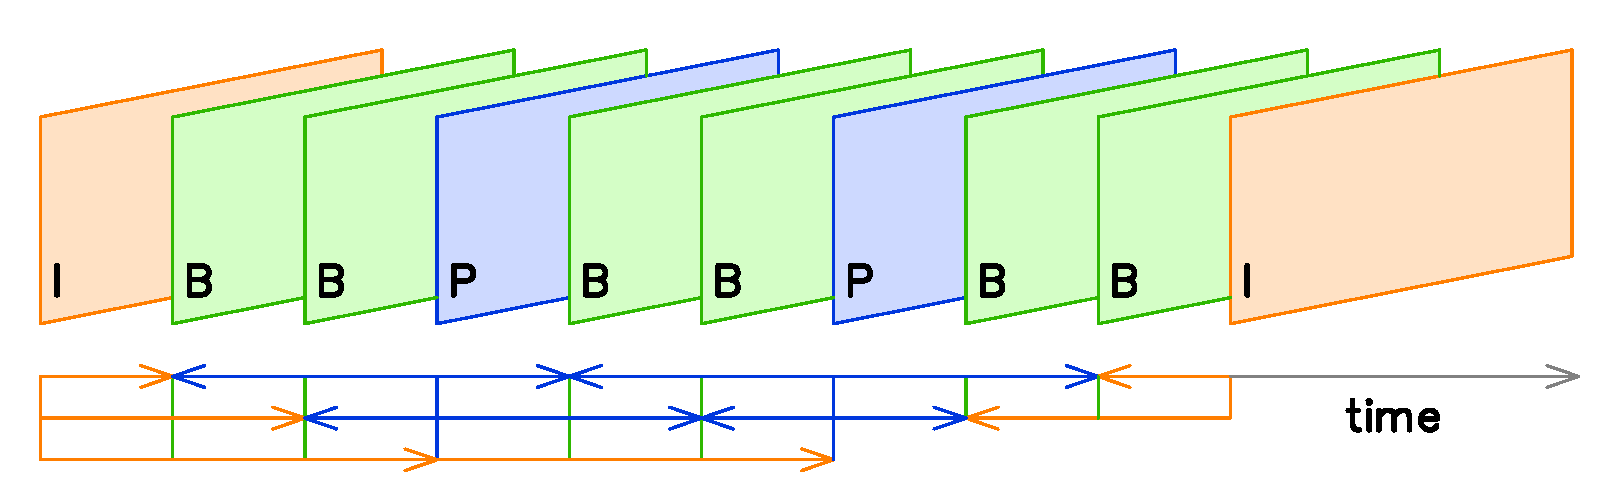
\includegraphics[width=0.7\textwidth, height=0.7\textheight, keepaspectratio]{img/IPB_images_sequence.png}}
\caption{An example of interleaved I-, B- and P-frames representing a video stream. The encoder may choose a different sequence of frame types. Reproduced from~\cite{interframe-wiki}.}
\label{fig:ipb-seq}
\end{figure}

A frame which will be encoded as a P-frame is partitioned into blocks of size 16-by-16 pixels\footnote{H.264 allows higher granularity for fine details by allowing some blocks to be 8x8, 8x16 or 16x8.}. These blocks are called \emph{macroblocks}, and for each macroblock the encoder searches for its most similar match in a predecessor frame (within a bounded search window) \cite[p.~256]{richardson2004h}. The difference in pixels between the matched block and the original is called the \emph{prediction error}, and the displacement between the two is called the \emph{motion vector} [Fig.~\ref{fig:mb-search}]. For simplicity, we say that a block of pixels has moved since the predecessor frame by the amount specified by its motion vector and, in addition to motion, pixels themselves have changed according to the prediction error.

\begin{figure}[tbh]
\centerline{\includegraphics[width=0.7\textwidth,height=0.7\textheight,keepaspectratio]
{img/macroblock-diagram.png}}
\caption{An illustration of a macroblock search from the current (target) frame to the predecessor (reference) frame. A macroblock is encoded using its prediction error and  motion vector.}
\label{fig:mb-search}
\end{figure} 

\subsection{Motion vectors as embedding space}

Computing motion vectors is a tradeoff between accuracy and computation time, tuned using the search window size. As such, codecs typically use an approximation instead of a globally optimal MV, resulting in a non-minimal prediction error \cite[p.~257]{richardson2004h}. While the MVs are encoded losslessly, the accuracy error allows minor changes to go unnoticed, making them suitable for LSB steganography (see \ref{lsb-steg}).

To estimate the embedding capacity, we generalise how all implemented embedding schemes should operate on motion vectors. Suppose an embedding scheme processes every motion vector in a grid individually for every frame and has an associated selection function $f$ which provides a number of bits that can be embedded into a particular motion vector. Later on, this function will allow to conveniently define a MV selection criteria for different embedding schemes.

\begin{definition}{Embedding capacity for video}

Let $M$ be an embedding scheme with an associated function $f_M : \mathbb{R}^2 \rightarrow \mathbb{N}$, which calculates how many bits can be embedded into a particular motion vector $\overrightarrow{mv} \in \mathbb{R}^2$. Then for an MPEG-encoded video $V$, the embedding capacity $\mathcal{C}_{V, M}$ is defined as:

$$ \mathcal{C}_{V, M} = \sum_{p \in \text{P-frames}(V)} \: \sum^{H}_{j = 0} \sum^{W}_{i = 0} f_M(\overrightarrow{mv}^p_{i, j})$$

where $W$ and $H$ are width and height of the macroblock grid, P-frames$(V)$ is a set of all P-frames of a video $V$ and $\overrightarrow{mv}^p_{i, j}$ is the MV of a macroblock  in $i$-th row and $j$-th column of the frame $p$.

\end{definition}

To see whether videos could generally hold a non-negligible amount of hidden data, one can estimate $\mathcal{C}_{V, M}$ by taking a product of the number of P-frames, the total number of MVs per frame and the average number of bits embedded per MV. For instance, an average HD video could reasonably have 6--15 P-frames per second\footnote{Depends on how often the encoder decides to use B-frames and I-frames. P-frames are better for video streaming as they do not require the successor frame during decoding.} with 3600 MVs each\footnote{If video's resolution is 1280x720 (HD), 16x16 macroblocks would partition the frame into a grid of size 80x45. This gives 3600 macroblocks in total.}. Assuming only a quarter of each frame would contain embedded data, I estimate the channel's capacity to be 5.4--13 Kbits/s. Since videos contain audio tracks and a higher number of pixels (or DCT coefficients) than images, a video file typically has higher embedding capacity than an audio file or an image.

\section{Requirements analysis}

The project has two main software deliverables:
\begin{itemize}
\item  An application that allows a user to embed secret messages into MPEG video files using a selection of LSB embedding algorithms.
\item A steganalysis suite that implements some general-purpose routines to detect motion vector-based steganography.
\end{itemize}

Below is a list of requirements for both deliverables, prioritised using \emph{MoSCoW} criteria~\cite{softid-notes}.

\subsection{Steganographic Application}
\begin{itemize}
\item (M) Ability to access motion vectors of an MPEG video file.
\item (M) Ability to reliably embed data within motion vectors.
\item (M) Multiple LSB embedding techniques.
\item (M) User-friendly binaries to perform embedding and extraction.
\item (S) Encryption of the secret message prior to embedding.
\item (S) Integration with an existing video codec.
\end{itemize}

\subsection{Steganalysis Suite}
\begin{itemize}
\item (M) Ability to extract and process motion vector data.
\item (M) Multiple steganalysis methods.
\item (M) Documentation on usage and interpretation of the results.
\item (M) Evident effectiveness in detecting implemented embedding techniques.
\item (S) Compatibility with existing scientific computation packages (Matlab or Python-based packages)
\item (S) Usefulness (verbosity, amount of information provided) to the steganalyst.
\end{itemize}

\section{Project workflow}

\subsection{Technical choices}

The steganographic application requires modifying MPEG video files, which in turn requires parsing the format of a file, modifying motion vector values, and repackaging the data back into a playable video. Developing a codec does not relate to steganography and is potentially error-prone, so I leverage an existing set of codecs---\texttt{FFmpeg}\footnote{\url{https://www.ffmpeg.org/}}---to achieve this. As codecs are typically written in C or C++, it is a natural choice for this task to and makes the integration easier.

Performing encryption prior to embedding requires using a cryptography library. I chose \emph{Crypto++}, a popular C++ cryptography library.

The steganalysis suite was integrated into the Matlab scientific computation package for user's benefit, because it provides useful tools, such as statistical primitives, plotting capabilities and classifiers, without changing the environment. I chose Matlab  because of its widespread use and comprehensive functionality.

\subsection{Risk analysis}
FFmpeg is a complex piece of software, mostly written in a style of C that sacrifices clarity for performance. A potential risk for the project was the difficulty of proper integration with FFmpeg and hence inability to access or reliably modify motion vectors. Complete failure to do so was unlikely, but it could have consumed a significant amount of development time. To mitigate this, some ``catch-up'' time was allocated in the project timetable.  

\subsection{Workflow}
\begin{itemize}
\item \emph{Git} was used for version control, allowing quick roll-back and managing multiple source trees using branches.
\item \emph{Backups} were done by uploading the source tree and other relevant files to Dropbox. The git repository itself was hosted remotely on GitHub.
\item \emph{Testing} \textbf{TODO}
\item \emph{Interative (spiral) development model} was used to continuously add and test new embedding schemes and steganalysis methods.
\end{itemize}

\section{Starting Point}
This project uses some cryptography concepts introduced in the Part IB \textit{Security I} course. I have had some C++ knowledge from past programming experience and the \textit{Programming in C and C++} course. 

Prior to submitting the proposal, I have familiarised myself with the general concepts of steganography and LSB embedding though some introductory texts and relevant papers, and briefly looked at H.264 codec format.

During the development of this project I made use of some material covered in the following Part II courses:
\begin{itemize}
\item \textit{Information Theory} --- channel capacity, error correcting codes;
\item \textit{\LaTeX~and Matlab} --- typesetting and basics of Matlab;
\item \textit{Artificial Intelligence II} --- classifier evaluation.
\end{itemize}

\bigskip
This chapter summarised relevant theoretical and practical background necessary to start the implementation. Next chapter will cover the design and features of the system, implemented steganographic algorithms and steganalysis methods, together with some in-line evaluation.

% Implementation
\cleardoublepage
\chapter{Implementation}

\textit{Lorem ipsum dolor sit amet, consectetur adipiscing elit. Vivamus vel nibh in est consectetur lobortis sit amet eu nisl. Morbi interdum ipsum vitae ligula rutrum vehicula. Mauris sagittis diam a cursus mollis. Nullam vel sapien erat. Vestibulum ut interdum dolor. Maecenas efficitur felis sapien, at sagittis tellus porta vel. Nam ac finibus metus. Nam vulputate ligula ac elementum vehicula.}

\section{Steganographic Application}

\subsection{Integration with FFmpeg}

Finding a suitable way of integrating with FFmpeg was one of the biggest challenges that the project faced at the beginning of development. FFmpeg is split into several libraries, each for a dedicated purpose, such as stream multiplexing, resampling and supporting I/O devices. The most suitable library to integrate the project with was \texttt{libavcodec} which implements various audio and video codecs. I decided to focus on H.264, as it is the most popular codec online; FFmpeg offloads it to a separate library --- \texttt{libx264}. The \texttt{libavcodec} library exposes an API to run the codecs it implements, but further investigation showed that it is not possible to manipulate motion vectors through it. Therefore, the next step was to modify the library to either introduce an additional API or call steganographic routines directly.

Initially, I was looking for a point in the macroblock search phase where motion vectors would already be available, but the prediction error would not have been computed yet. This would allow modifying MVs without any visual footprint because prediction error would have brought the pixels to their required values regardless of the motion vector's value. However, since both FFmpeg and \texttt{libx264} are projects with a complex data flow, written in C with high performance in mind, analysing them has been more difficult than initially anticipated. As a result of this, the project got delayed by 4 weeks with respect to the original timeline, so the following measures have been taken to quickly resolve this obstacle:
\begin{itemize}
\item Choosing the codec that's fully contained within \texttt{libavcodec}, so that \texttt{libx264} does not have to be used at all. I chose MPEG-4 Part 2 (\texttt{xvid}), H.264's popular predecessor.
\item Focus on modifying motion vectors, because it is essential to the project. Macroblock search is contained deep within the encoding pipeline, which makes modifying it less approachable. Instead, I have been able to modify motion vectors before they are written to the output file.
\end{itemize}

However, this left prediction errors untouched, so an experiment on human subjects was conducted to ensure this still does not result in a noticeable visual footprint.  

\subsection{Steganography Library}

\subsubsection{C API}

To achieve a modular design and decouple from FFmpeg, steganographic algorithms were separated into a standalone library \texttt{movestlib}\footnote{\texttt{movest} (\underline{mo}tion \underline{ve}ctor \underline {st}eganography) is the codename for this project.}. Library itself is implemented in C++ and exposes a C API for integration with FFmpeg, and encoder and decoder applications (Figure \ref{fig:movest-c-api}). Exact operation of these methods is described later in section \ref{enc-dec-bin} using these applications as examples.

\begin{figure}[tbh]
\centerline{\includegraphics[width=0.85\textwidth, height=\textheight, keepaspectratio]{img/movest_c_api.png}}
\caption{UML diagram of the C API provided by \texttt{movestlib}. (Some method parameters omitted for brevity.)}
\label{fig:movest-c-api}
\end{figure}

\subsubsection{Class hierarchy}

The class hierarchy of embedding algorithms is presented in Figure \ref{fig:movest_alg_class_diag}. \texttt{Algorithm} is the base class for all embedding algorithms and contains common functionality, such as setting up the payload file or operating on every motion vector of a suitable type in turn. Most algorithms, however, extend \texttt{HideSeek} to benefit from the following more specific functionality:
\begin{itemize}
\item Operating on a per-component basis. Motion vectors are stored as $x$ and $y$ components and many algorithms treat them independently. (\texttt{RandomisedHideSeek, OutGuess1})
\item Sequential data fetching and stopping criteria. Some algorithms read and embed payload bits sequentially and require knowing when to stop the embedding process. (\texttt{XuAlg, MVSteg})
\item Both of above. (\texttt{MSteg, F3, F4})
\end{itemize}

\begin{figure}[tbh]
\centerline{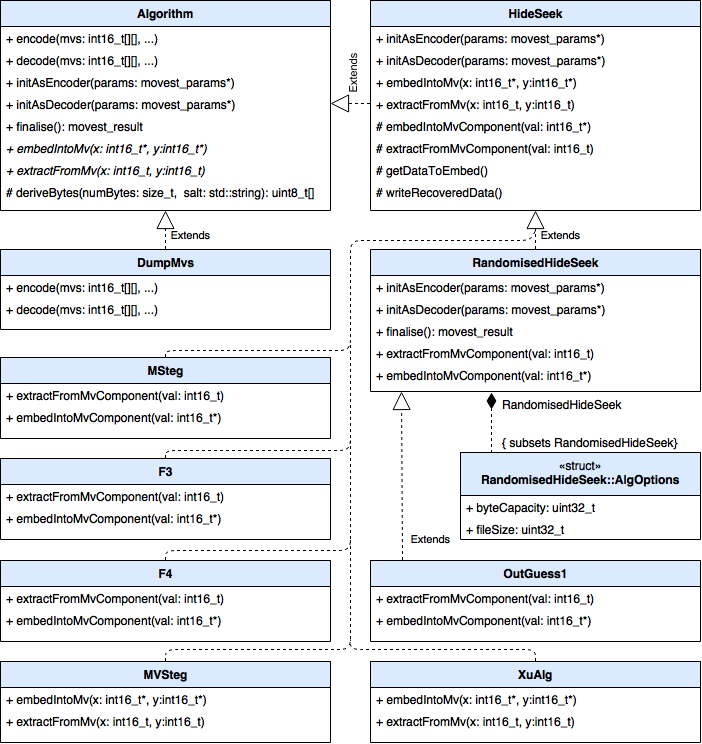
\includegraphics[width=0.85\textwidth, height=\textheight, keepaspectratio]{img/movest_alg_class_diag.png}}
\caption{UML diagram of embedding algorithms implemented in \texttt{movestlib}. (Some unimportant fields, methods and method parameters omitted for brevity.)}
\label{fig:movest_alg_class_diag}
\end{figure}

A singleton instance of an embedding algorithm is kept active after initialisation. FFmpeg feeds motion vector data into the algorithm by calling C API methods \texttt{movest\_encode/decode}.  

\subsubsection{Encryption}
Encrypting the payload hides the structure of the data by making it indistinguishable from random noise, also making it hard to detect in already-noisy regions. An additional benefit of the encryption is that the embedded data will remain unreadable by an adversary even if steganography was broken. \texttt{movestlib} achieves this by implementing a file-like object for accessing the payload, and encrypting or decrypting the data on the fly (\texttt{MOVEST\_ENCRYPTION} flag). I made the choice in favour of well-established AES encryption in counter (CTR) mode with a 256-bit key. The key itself and the initialisation vector are derived from the user-supplied password by performing key stretching using an industry-standard PBKDF2-HMAC-SHA1 key derivation function. Manually implementing cryptographic primitives is error-prone and can lead to major security flaws, so the Crypto++ library is used to provide them. 

\subsection{Encoder and decoder applications}
\label{enc-dec-bin}
The project provides video-processing applications for embedding and recovering the payload from a video file. The two are largely based on FFmpeg examples for transcoding (\texttt{transcoding.c}) and motion vector extraction (\texttt{extract\_mvs.c}), which already contain the code to trigger code paths in FFmpeg that I have modified.

Before letting FFmpeg code to process the video, applications parse user's input to initialise \texttt{movestlib} with required data, such as the embedding algorithm (\texttt{movest\_init\_algorithm}), the payload file path and the encryption password (\texttt{movest\_init\_encoder/decoder}). FFmpeg treats sequences of frames as streams, which means that frames are written to the output file one after another and it is not possible to access a previous or a future frame during the embedding process. Algorithms that require estimating certain parameters, for example, the embedding capacity of a video prior to modifying it, have to make all embedding decisions in advance. To enable this, the encoder performs a dry run (\texttt{MOVEST\_DUMMY\_PASS} flag) for data collection --- motion vectors themselves are not modified in this case.

\textbf{sample help?}

\section{Steganalysis techniques}

Steganalysis techniques for this project were implemented in Matlab, which allowed to greatly simplify the implementation by leveraging existing data processing, plotting and statistical routines. All techniques will be shown in action against implemented algorithms.

\subsection{Motion vector import}
\label{mv-import}

Decoder application can be set up to use a special algorithm \texttt{DumpMvs} which will output motion vector components using an easy-to-parse text format. Matlab can later import this data as 3D matrices (\texttt{loadmvs.m}), where element at $(i, j, k)$ refers to a macroblock at $i$-th row, $j$-th column of the $k$-th frame. 

The codec allows some macroblocks to be completely omitted. These are called ``skip" macroblocks, and Movest decoder assigns them a special type during extraction. In this case, for the sake of completeness of the grid, FFmpeg reports the motion vector being $(0, 0)$, but a user can filter out such stray zeros by using type information (\texttt{typedmvs.m}).

\subsection{LSB plane, 2D plotting and aggregation into bytes}

This project implements LSB steganography, so the suite includes a function (\texttt{lsbplane.m}) to project least significant bits out of every motion vector component value. If the embedding algorithm sets LSBs of motion vectors to exactly payload bits, LSBs can be immediately subjected to visual analysis to reveal any patterns in the data. This is best illustrated by an example.

\begin{figure}[tbh]
\centerline{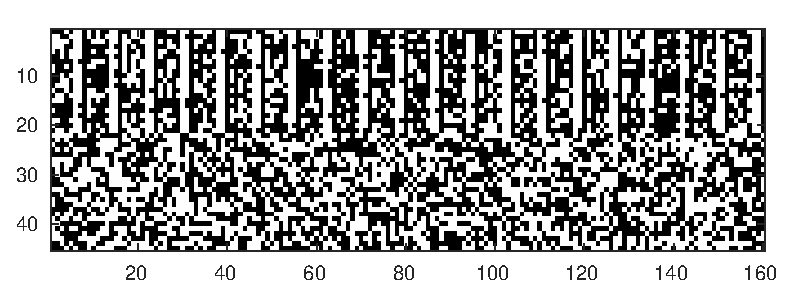
\includegraphics{img/unencrypted-enc.eps}}
\caption{Sample output of \texttt{plot2d} over LSB plane. Even-numbered and odd-numbered columns contain LSBs for $x$ and $y$ components respectively.}
\label{fig:unencrypted-enc}
\end{figure}

Figure \ref{fig:unencrypted-enc} shows an example of 2-valued heatmap (\texttt{plot2d.m}) produced by the suite. The plot shows a clear pattern of embedded data in the first half of the frame. Given that there are repeating columns of 1s every 8 bits, steganalyst can make an educated guess that the payload is ASCII-encoded and attempt to group bits into bytes to reproduce the text (\texttt{aggregateIntoBytes.m}):

\begin{alltt}
    >> char\footnote{In Matlab, \texttt{char} interprets an integer value as an ASCII-encoded character.}(aggregateIntoBytes(mvs, types))'
    ans = hello world\ldots
\end{alltt}

\subsection{Histogram and $\chi^2$ (Chi-Squared) Attack}

The distribution of motion vectors can be visualised using a histogram (\texttt{mvhist.m}). This can be a useful source of information for a steganalyst because peculiarities in the histogram can reveal that motion vectors have been modified. Typically MV histograms have a sharp peak at 0 and exponentially decay on both sides, with decay rates, additional peaks and plateaus depending on the most common direction of motion in the video (Figure \ref{fig:histogram-example}). 

\begin{figure}[tbh]
\centerline{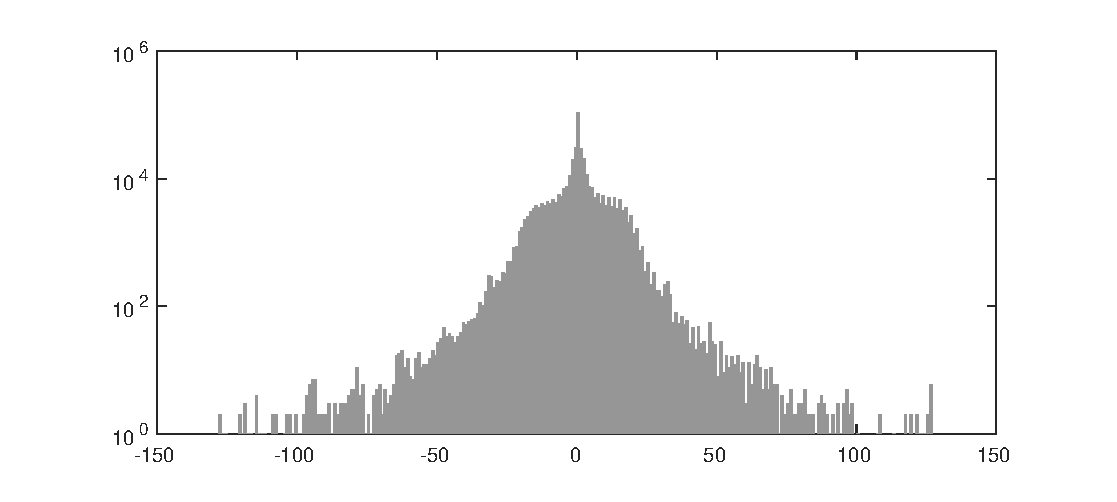
\includegraphics[scale=0.75]{img/histogram-example.eps}}
\caption{Sample output of \texttt{mvhist} for the $x$ component of all motion vectors in a video.}
\label{fig:histogram-example}
\end{figure}

In a method, originally developed for attacking image steganography, Westfeld and Pfitzmann~\cite{westfeld1999attacks} hypothesise that due to the nature of data it is  unlikely that adjacent bars of the histogram would be of the same height. Consider adjacent bars on a histogram which correspond to even-odd pairs of motion vector values that only differ in the LSB (0 and 1, 2 and 3, 4 and 5, \emph{etc.}). The rationale behind the \emph{$\chi^2$ attack} is that the (encrypted) payload will have the same number of 0 and 1 bits on average, and  because LSBs of motion vector values are identical to payload bits, values in an even-odd pair should occur the same number of times. This also implies that histogram bars for an even-odd pair should be of the same height. 

We can now devise a statistical procedure (\texttt{chiSquareAttack.m}) which can tell with a certain probability whether motion vectors contain a secret message. As described above, we consider even-odd pairs of motion vector values of the form $(2k, 2k+1)$. 

Let $X_k$ and $Y_k$ be the number of times values $2k$ and $2k+1$ occur as motion vector values respectively. Let us also consider another variable $Z_k = \frac{X_k + Y_k}{2}$ --- the average of the two. If the video contains the payload, $X_k$ and $Y_k$ should be almost equal, or, in other words, be distributed as $Z_k$. To prevent influence from the noise in data, pairs that have $Z_k < 8$ are considered to be under-represented and are neglected in further analysis (\emph{minimum frequency condition}). \textbf{address the difference from the paper?}

We can use the \emph{$\chi^2$ (chi-square) test} to check the hypothesis that there is no significant difference between $X_k$ and $Z_k$ (null hypothesis). The case for $Y_k$ is symmetric and not considered further. The test tells us we can compute the quantity

$$ \chi^2_{n-1} \approx \sum^{n}_{k=0} \frac{(\text{observed}_k - \text{expected}_k)^2}{\text{expected}_k}= \sum^{255}_{k=-255} \frac{(X_k - Z_k)^2}{Z_k} $$ 

from which we can obtain the $p$-value of data supporting the null hypothesis, which Westfeld and Pfitzmann interpret as the probability that the cover contains the payload \cite{westfeld1999attacks}:

$$ p = 1 - \frac{1}{2^{\frac{n-1}{2}}\Gamma(\frac{n-1}{2})}\int_0^{\chi^2_{n-1}}t^{\frac{n-1}{2}−1}e^{-t/2}dt $$  

This method can be further extended to estimate the size of the payload. From the expression for $\chi^2_{n-1}$, we see that it is sensitive so small changes --- value stays close to 0 when data contains the payload ($X_k - Z_k \approx 0$) and is big otherwise. We can iteratively build up the histogram and update $\chi^2_{n-1}$ as data for every frame comes in. We know that when the value starts increasing (and $p$-value decreases), data no longer contains the payload, so we can put a bound on the payload size. 

\subsection{Reversion Technique}
Cao \emph{et al.}~\cite{cao2012video} proves that decoding and re-encoding (transcoding) the video tends to remove the changes caused by embedding the payload. That is, motion vectors tend to revert to their original values. Therefore, if a video does not contain the payload, we expect differences between respective motion vectors of the original and transcoded video to be mostly low or zero, and if it does contain the payload, we expect larger differences to be more common.

\begin{wrapfigure}{R}{5.5cm}
\includegraphics[scale=0.7]{img/movest_reversion_sketch.png}
\caption{Partitioning stego and non-stego videos.}
\label{fig:movest-reversion-sketch}
\end{wrapfigure}

\emph{Sum of absolute differences (SAD)} is used to compute the difference between respective components of motion vectors:

$$ \Delta \overrightarrow{mv^p_{ij}} = |(\overrightarrow{o^p_{ij}})_x - (\overrightarrow{t^p_{ij}})_x| +  |(\overrightarrow{o^p_{ij}})_y - (\overrightarrow{t^p_{ij}})_y|$$

where $\overrightarrow{o^p_{ij}}$ and $\overrightarrow{t^p_{ij}}$ are motion vectors of the original and transcoded video. To assess how common small and large differences are in a video, we compute a normalised vector of frequencies for every value of $\Delta\overrightarrow{mv^p_{ij}}$. That is, $k$-th element of the vector tells the proportion of $\Delta\overrightarrow{mv^p_{ij}} = k$ occurring among all SADs.

The hypothesis suggests the following approach of distinguishing between a stego and non-stego video, summarised in Figure \ref{fig:movest-reversion-sketch}:
\begin{itemize}
\item Stego videos will have a lower frequency of small differences ($\Delta\overrightarrow{mv^p_{ij}} < 2$), but a higher frequency of larger differences ($\Delta\overrightarrow{mv^p_{ij}} \geq 2$).
\item Non-stego videos will have a higher frequency of small differences and a lower frequency of larger differences.
\end{itemize}

Therefore, we can build a classifier which will try to learn the partition between two classes. I decided to use a Support Vector Machine (SVM) with linear kernel (as Figure \ref{fig:movest-reversion-sketch} suggests), trained using Matlab's \texttt{fitcsvm} routine.

\section{Embedding algorithms}
\label{emb-alg}

The project implements 7 embedding algorithms which are presented in this section together with some in-line evaluation justifying design choices.

\subsection{Hide \& Seek}

\emph{Hide \& Seek}~\cite{bateman} is the algorithm that was alluded to in the previous section. The algorithm embeds payload bits into both $x$ and $y$ components of each motion vector by setting their LSB to that of the payload. This achieves the maximal capacity for this kind of embedding --- 2 bits per macroblock. However, it is also susceptible to all attacks described in the previous section. 

Since data is embedded into all possible macroblocks, the visual analysis allows easily spotting it in a non-noisy region. Figure \ref{fig:visual-analysis-example} shows two 2D plots of the same frame: one without the embedding and one with data embedded at about 45\% of capacity. Unusual noise in the first half of the frame exposes the embedding.  

\begin{figure}[tbh]
\centerline{
\begin{subfigure}[t]{0.4\textwidth}
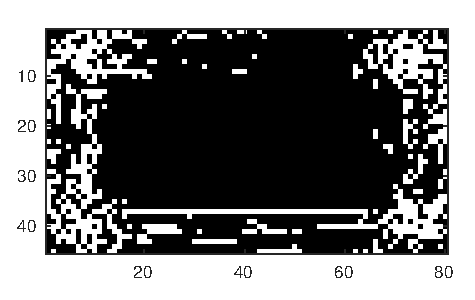
\includegraphics[scale=0.8]{img/pre-lsb-embedding.eps}
\end{subfigure}
~
\begin{subfigure}[t]{0.4\textwidth}
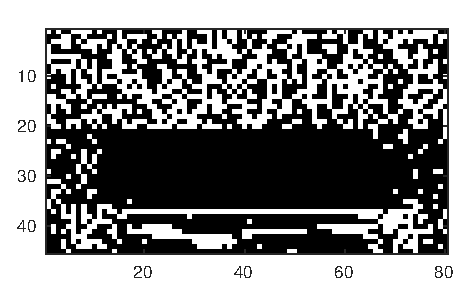
\includegraphics[scale=0.8]{img/post-lsb-embedding.eps}
\end{subfigure}
}
\caption{An example of a frame prior to embedding (left) and after embedding at 45\% capacity (right).}
\label{fig:visual-analysis-example}
\end{figure}

\subsection{MSteg}
\label{msteg}

\emph{MSteg} is my straightforward adaptation of the \emph{JSteg} algorithm~\cite{bateman}, which was initially developed for embedding into JPEG DCT coefficients. The algorithm operates in the same way as Hide \& Seek, but addresses the visual detection problem by not embedding into ``still'' regions, where noise would be easily detectable. From the implementation perspective, it avoids embedding bits into 0-valued $x$ and $y$ components. Components with value 1 are also avoided, since embedding bit 0 would turn them into zeros, making decoding ambiguous.

Figure \ref{fig:msteg-visual} shows that MSteg performs better when subjected to visual analysis. However, we would still expect values in an even-odd pair occur at the same frequency, as described earlier. Histogram in Figure \ref{fig:msteg-hist} confirms this and therefore the $\chi^2$ attack is successful at detecting the embedding (Figure \ref{fig:chisq-attack}).

\begin{figure}[tbh]
\centering
\begin{minipage}[t]{.4\textwidth}
  \centering
  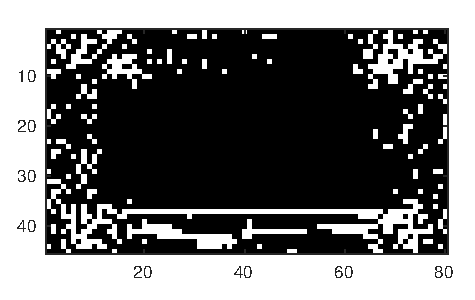
\includegraphics[scale=0.8]{img/msteg-visual.eps}
  \caption{LSB plane of the frame subjected to MSteg embedding.}
  \label{fig:msteg-visual}
\end{minipage}%
\quad\quad
\begin{minipage}[t]{.45\textwidth}
  \centering
  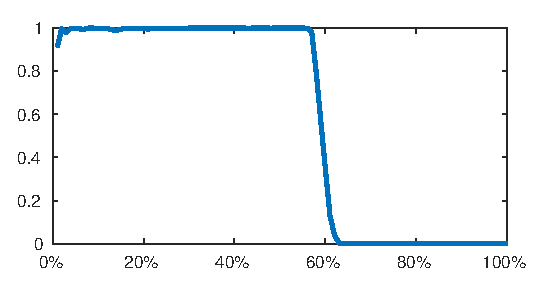
\includegraphics[scale=0.84]{img/chisq-attack.eps}
  \caption{An example of probability of embedding computed by the $\chi^2$ attack when embedding was done at 58\% of capacity.}
  \label{fig:chisq-attack}
\end{minipage}
\end{figure}

\begin{figure}[tbh]
\centering
\resizebox{0.6\textwidth}{!}{%LaTeX with PSTricks extensions
%%Creator: inkscape 0.91
%%Please note this file requires PSTricks extensions
\psset{xunit=.5pt,yunit=.5pt,runit=.5pt}
\begin{pspicture}(349,154)
{
\newrgbcolor{curcolor}{1 1 1}
\pscustom[linestyle=none,fillstyle=solid,fillcolor=curcolor]
{
\newpath
\moveto(0,154)
\lineto(349,154)
\lineto(349,0)
\lineto(0,0)
\closepath
}
}
{
\newrgbcolor{curcolor}{1 1 1}
\pscustom[linestyle=none,fillstyle=solid,fillcolor=curcolor]
{
\newpath
\moveto(0,154)
\lineto(349,154)
\lineto(349,0)
\lineto(0,0)
\closepath
}
}
{
\newrgbcolor{curcolor}{1 1 1}
\pscustom[linestyle=none,fillstyle=solid,fillcolor=curcolor]
{
\newpath
\moveto(25,20)
\lineto(349,20)
\lineto(349,138)
\lineto(25,138)
\closepath
}
}
{
\newrgbcolor{curcolor}{0.14901961 0.14901961 0.14901961}
\pscustom[linewidth=0.66670001,linecolor=curcolor]
{
\newpath
\moveto(25,20)
\lineto(349,20)
}
}
{
\newrgbcolor{curcolor}{0.14901961 0.14901961 0.14901961}
\pscustom[linewidth=0.66670001,linecolor=curcolor]
{
\newpath
\moveto(25,138)
\lineto(349,138)
}
}
{
\newrgbcolor{curcolor}{0.14901961 0.14901961 0.14901961}
\pscustom[linewidth=0.66670001,linecolor=curcolor]
{
\newpath
\moveto(39.72729874,20)
\lineto(39.72729874,23.24000549)
}
}
{
\newrgbcolor{curcolor}{0.14901961 0.14901961 0.14901961}
\pscustom[linewidth=0.66670001,linecolor=curcolor]
{
\newpath
\moveto(113.36360168,20)
\lineto(113.36360168,23.24000549)
}
}
{
\newrgbcolor{curcolor}{0.14901961 0.14901961 0.14901961}
\pscustom[linewidth=0.66670001,linecolor=curcolor]
{
\newpath
\moveto(187,20)
\lineto(187,23.24000549)
}
}
{
\newrgbcolor{curcolor}{0.14901961 0.14901961 0.14901961}
\pscustom[linewidth=0.66670001,linecolor=curcolor]
{
\newpath
\moveto(260.63641357,20)
\lineto(260.63641357,23.24000549)
}
}
{
\newrgbcolor{curcolor}{0.14901961 0.14901961 0.14901961}
\pscustom[linewidth=0.66670001,linecolor=curcolor]
{
\newpath
\moveto(334.27270508,20)
\lineto(334.27270508,23.24000549)
}
}
{
\newrgbcolor{curcolor}{0.14901961 0.14901961 0.14901961}
\pscustom[linewidth=0.66670001,linecolor=curcolor]
{
\newpath
\moveto(39.72729874,138)
\lineto(39.72729874,134.76000023)
}
}
{
\newrgbcolor{curcolor}{0.14901961 0.14901961 0.14901961}
\pscustom[linewidth=0.66670001,linecolor=curcolor]
{
\newpath
\moveto(113.36360168,138)
\lineto(113.36360168,134.76000023)
}
}
{
\newrgbcolor{curcolor}{0.14901961 0.14901961 0.14901961}
\pscustom[linewidth=0.66670001,linecolor=curcolor]
{
\newpath
\moveto(187,138)
\lineto(187,134.76000023)
}
}
{
\newrgbcolor{curcolor}{0.14901961 0.14901961 0.14901961}
\pscustom[linewidth=0.66670001,linecolor=curcolor]
{
\newpath
\moveto(260.63641357,138)
\lineto(260.63641357,134.76000023)
}
}
{
\newrgbcolor{curcolor}{0.14901961 0.14901961 0.14901961}
\pscustom[linewidth=0.66670001,linecolor=curcolor]
{
\newpath
\moveto(334.27270508,138)
\lineto(334.27270508,134.76000023)
}
}
{
\newrgbcolor{curcolor}{0.14901961 0.14901961 0.14901961}
\pscustom[linestyle=none,fillstyle=solid,fillcolor=curcolor]
{
\newpath
\moveto(30.3132375,6.79057812)
\lineto(33.47144062,6.79057812)
\lineto(33.47144062,5.82964062)
\lineto(30.3132375,5.82964062)
\lineto(30.3132375,6.79057812)
\closepath
}
}
{
\newrgbcolor{curcolor}{0.14901961 0.14901961 0.14901961}
\pscustom[linestyle=none,fillstyle=solid,fillcolor=curcolor]
{
\newpath
\moveto(36.36597187,4.01909375)
\lineto(40.49683125,4.01909375)
\lineto(40.49683125,3.023)
\lineto(34.94214375,3.023)
\lineto(34.94214375,4.01909375)
\curveto(35.3913625,4.4839375)(36.00269062,5.10698437)(36.77612812,5.88823437)
\curveto(37.55347187,6.67339062)(38.04175312,7.17925)(38.24097187,7.4058125)
\curveto(38.61987812,7.83159375)(38.88355,8.19096875)(39.0319875,8.4839375)
\curveto(39.18433125,8.7808125)(39.26050312,9.07182812)(39.26050312,9.35698437)
\curveto(39.26050312,9.82182812)(39.09644062,10.20073437)(38.76831562,10.49370312)
\curveto(38.44409687,10.78667187)(38.02026875,10.93315625)(37.49683125,10.93315625)
\curveto(37.1257375,10.93315625)(36.73315937,10.86870312)(36.31909687,10.73979687)
\curveto(35.90894062,10.61089062)(35.4694875,10.41557812)(35.0007375,10.15385937)
\lineto(35.0007375,11.34917187)
\curveto(35.4773,11.54057812)(35.9226125,11.68510937)(36.336675,11.78276562)
\curveto(36.7507375,11.88042187)(37.12964375,11.92925)(37.47339375,11.92925)
\curveto(38.37964375,11.92925)(39.1023,11.7026875)(39.6413625,11.2495625)
\curveto(40.180425,10.7964375)(40.44995625,10.19096875)(40.44995625,9.43315625)
\curveto(40.44995625,9.07378125)(40.38159687,8.73198437)(40.24487812,8.40776562)
\curveto(40.11206562,8.08745312)(39.867925,7.70854687)(39.51245625,7.27104687)
\curveto(39.4148,7.15776562)(39.10425312,6.82964062)(38.58081562,6.28667187)
\curveto(38.05737812,5.74760937)(37.31909687,4.99175)(36.36597187,4.01909375)
\closepath
}
}
{
\newrgbcolor{curcolor}{0.14901961 0.14901961 0.14901961}
\pscustom[linestyle=none,fillstyle=solid,fillcolor=curcolor]
{
\newpath
\moveto(45.51831562,10.99175)
\curveto(44.90894062,10.99175)(44.44995625,10.69096875)(44.1413625,10.08940625)
\curveto(43.836675,9.49175)(43.68433125,8.59135937)(43.68433125,7.38823437)
\curveto(43.68433125,6.18901562)(43.836675,5.288625)(44.1413625,4.6870625)
\curveto(44.44995625,4.08940625)(44.90894062,3.79057812)(45.51831562,3.79057812)
\curveto(46.13159687,3.79057812)(46.59058125,4.08940625)(46.89526875,4.6870625)
\curveto(47.2038625,5.288625)(47.35815937,6.18901562)(47.35815937,7.38823437)
\curveto(47.35815937,8.59135937)(47.2038625,9.49175)(46.89526875,10.08940625)
\curveto(46.59058125,10.69096875)(46.13159687,10.99175)(45.51831562,10.99175)
\closepath
\moveto(45.51831562,11.92925)
\curveto(46.49878437,11.92925)(47.24683125,11.54057812)(47.76245625,10.76323437)
\curveto(48.2819875,9.98979687)(48.54175312,8.86479687)(48.54175312,7.38823437)
\curveto(48.54175312,5.91557812)(48.2819875,4.79057812)(47.76245625,4.01323437)
\curveto(47.24683125,3.23979687)(46.49878437,2.85307812)(45.51831562,2.85307812)
\curveto(44.53784687,2.85307812)(43.78784687,3.23979687)(43.26831562,4.01323437)
\curveto(42.75269062,4.79057812)(42.49487812,5.91557812)(42.49487812,7.38823437)
\curveto(42.49487812,8.86479687)(42.75269062,9.98979687)(43.26831562,10.76323437)
\curveto(43.78784687,11.54057812)(44.53784687,11.92925)(45.51831562,11.92925)
\closepath
}
}
{
\newrgbcolor{curcolor}{0.14901961 0.14901961 0.14901961}
\pscustom[linestyle=none,fillstyle=solid,fillcolor=curcolor]
{
\newpath
\moveto(103.9495375,6.79057812)
\lineto(107.10774063,6.79057812)
\lineto(107.10774063,5.82964062)
\lineto(103.9495375,5.82964062)
\lineto(103.9495375,6.79057812)
\closepath
}
}
{
\newrgbcolor{curcolor}{0.14901961 0.14901961 0.14901961}
\pscustom[linestyle=none,fillstyle=solid,fillcolor=curcolor]
{
\newpath
\moveto(109.18781875,4.01909375)
\lineto(111.1214125,4.01909375)
\lineto(111.1214125,10.69292187)
\lineto(109.01789688,10.27104687)
\lineto(109.01789688,11.34917187)
\lineto(111.10969375,11.77104687)
\lineto(112.2932875,11.77104687)
\lineto(112.2932875,4.01909375)
\lineto(114.22688125,4.01909375)
\lineto(114.22688125,3.023)
\lineto(109.18781875,3.023)
\lineto(109.18781875,4.01909375)
\closepath
}
}
{
\newrgbcolor{curcolor}{0.14901961 0.14901961 0.14901961}
\pscustom[linestyle=none,fillstyle=solid,fillcolor=curcolor]
{
\newpath
\moveto(119.15461563,10.99175)
\curveto(118.54524063,10.99175)(118.08625625,10.69096875)(117.7776625,10.08940625)
\curveto(117.472975,9.49175)(117.32063125,8.59135937)(117.32063125,7.38823437)
\curveto(117.32063125,6.18901562)(117.472975,5.288625)(117.7776625,4.6870625)
\curveto(118.08625625,4.08940625)(118.54524063,3.79057812)(119.15461563,3.79057812)
\curveto(119.76789688,3.79057812)(120.22688125,4.08940625)(120.53156875,4.6870625)
\curveto(120.8401625,5.288625)(120.99445938,6.18901562)(120.99445938,7.38823437)
\curveto(120.99445938,8.59135937)(120.8401625,9.49175)(120.53156875,10.08940625)
\curveto(120.22688125,10.69096875)(119.76789688,10.99175)(119.15461563,10.99175)
\closepath
\moveto(119.15461563,11.92925)
\curveto(120.13508438,11.92925)(120.88313125,11.54057812)(121.39875625,10.76323437)
\curveto(121.9182875,9.98979687)(122.17805313,8.86479687)(122.17805313,7.38823437)
\curveto(122.17805313,5.91557812)(121.9182875,4.79057812)(121.39875625,4.01323437)
\curveto(120.88313125,3.23979687)(120.13508438,2.85307812)(119.15461563,2.85307812)
\curveto(118.17414688,2.85307812)(117.42414688,3.23979687)(116.90461563,4.01323437)
\curveto(116.38899063,4.79057812)(116.13117813,5.91557812)(116.13117813,7.38823437)
\curveto(116.13117813,8.86479687)(116.38899063,9.98979687)(116.90461563,10.76323437)
\curveto(117.42414688,11.54057812)(118.17414688,11.92925)(119.15461563,11.92925)
\closepath
}
}
{
\newrgbcolor{curcolor}{0.14901961 0.14901961 0.14901961}
\pscustom[linestyle=none,fillstyle=solid,fillcolor=curcolor]
{
\newpath
\moveto(186.81445312,10.99175)
\curveto(186.20507812,10.99175)(185.74609375,10.69096875)(185.4375,10.08940625)
\curveto(185.1328125,9.49175)(184.98046875,8.59135937)(184.98046875,7.38823437)
\curveto(184.98046875,6.18901562)(185.1328125,5.288625)(185.4375,4.6870625)
\curveto(185.74609375,4.08940625)(186.20507812,3.79057812)(186.81445312,3.79057812)
\curveto(187.42773438,3.79057812)(187.88671875,4.08940625)(188.19140625,4.6870625)
\curveto(188.5,5.288625)(188.65429688,6.18901562)(188.65429688,7.38823437)
\curveto(188.65429688,8.59135937)(188.5,9.49175)(188.19140625,10.08940625)
\curveto(187.88671875,10.69096875)(187.42773438,10.99175)(186.81445312,10.99175)
\closepath
\moveto(186.81445312,11.92925)
\curveto(187.79492188,11.92925)(188.54296875,11.54057812)(189.05859375,10.76323437)
\curveto(189.578125,9.98979687)(189.83789062,8.86479687)(189.83789062,7.38823437)
\curveto(189.83789062,5.91557812)(189.578125,4.79057812)(189.05859375,4.01323437)
\curveto(188.54296875,3.23979687)(187.79492188,2.85307812)(186.81445312,2.85307812)
\curveto(185.83398438,2.85307812)(185.08398438,3.23979687)(184.56445312,4.01323437)
\curveto(184.04882812,4.79057812)(183.79101562,5.91557812)(183.79101562,7.38823437)
\curveto(183.79101562,8.86479687)(184.04882812,9.98979687)(184.56445312,10.76323437)
\curveto(185.08398438,11.54057812)(185.83398438,11.92925)(186.81445312,11.92925)
\closepath
}
}
{
\newrgbcolor{curcolor}{0.14901961 0.14901961 0.14901961}
\pscustom[linestyle=none,fillstyle=solid,fillcolor=curcolor]
{
\newpath
\moveto(254.12468125,4.01909375)
\lineto(256.058275,4.01909375)
\lineto(256.058275,10.69292187)
\lineto(253.95475937,10.27104687)
\lineto(253.95475937,11.34917187)
\lineto(256.04655625,11.77104687)
\lineto(257.23015,11.77104687)
\lineto(257.23015,4.01909375)
\lineto(259.16374375,4.01909375)
\lineto(259.16374375,3.023)
\lineto(254.12468125,3.023)
\lineto(254.12468125,4.01909375)
\closepath
}
}
{
\newrgbcolor{curcolor}{0.14901961 0.14901961 0.14901961}
\pscustom[linestyle=none,fillstyle=solid,fillcolor=curcolor]
{
\newpath
\moveto(264.09147812,10.99175)
\curveto(263.48210312,10.99175)(263.02311875,10.69096875)(262.714525,10.08940625)
\curveto(262.4098375,9.49175)(262.25749375,8.59135937)(262.25749375,7.38823437)
\curveto(262.25749375,6.18901562)(262.4098375,5.288625)(262.714525,4.6870625)
\curveto(263.02311875,4.08940625)(263.48210312,3.79057812)(264.09147812,3.79057812)
\curveto(264.70475937,3.79057812)(265.16374375,4.08940625)(265.46843125,4.6870625)
\curveto(265.777025,5.288625)(265.93132187,6.18901562)(265.93132187,7.38823437)
\curveto(265.93132187,8.59135937)(265.777025,9.49175)(265.46843125,10.08940625)
\curveto(265.16374375,10.69096875)(264.70475937,10.99175)(264.09147812,10.99175)
\closepath
\moveto(264.09147812,11.92925)
\curveto(265.07194687,11.92925)(265.81999375,11.54057812)(266.33561875,10.76323437)
\curveto(266.85515,9.98979687)(267.11491562,8.86479687)(267.11491562,7.38823437)
\curveto(267.11491562,5.91557812)(266.85515,4.79057812)(266.33561875,4.01323437)
\curveto(265.81999375,3.23979687)(265.07194687,2.85307812)(264.09147812,2.85307812)
\curveto(263.11100937,2.85307812)(262.36100937,3.23979687)(261.84147812,4.01323437)
\curveto(261.32585312,4.79057812)(261.06804062,5.91557812)(261.06804062,7.38823437)
\curveto(261.06804062,8.86479687)(261.32585312,9.98979687)(261.84147812,10.76323437)
\curveto(262.36100937,11.54057812)(263.11100937,11.92925)(264.09147812,11.92925)
\closepath
}
}
{
\newrgbcolor{curcolor}{0.14901961 0.14901961 0.14901961}
\pscustom[linestyle=none,fillstyle=solid,fillcolor=curcolor]
{
\newpath
\moveto(328.57543437,4.01909375)
\lineto(332.70629375,4.01909375)
\lineto(332.70629375,3.023)
\lineto(327.15160625,3.023)
\lineto(327.15160625,4.01909375)
\curveto(327.600825,4.4839375)(328.21215312,5.10698437)(328.98559062,5.88823437)
\curveto(329.76293437,6.67339062)(330.25121562,7.17925)(330.45043437,7.4058125)
\curveto(330.82934062,7.83159375)(331.0930125,8.19096875)(331.24145,8.4839375)
\curveto(331.39379375,8.7808125)(331.46996562,9.07182812)(331.46996562,9.35698437)
\curveto(331.46996562,9.82182812)(331.30590312,10.20073437)(330.97777812,10.49370312)
\curveto(330.65355937,10.78667187)(330.22973125,10.93315625)(329.70629375,10.93315625)
\curveto(329.3352,10.93315625)(328.94262187,10.86870312)(328.52855937,10.73979687)
\curveto(328.11840312,10.61089062)(327.67895,10.41557812)(327.2102,10.15385937)
\lineto(327.2102,11.34917187)
\curveto(327.6867625,11.54057812)(328.132075,11.68510937)(328.5461375,11.78276562)
\curveto(328.9602,11.88042187)(329.33910625,11.92925)(329.68285625,11.92925)
\curveto(330.58910625,11.92925)(331.3117625,11.7026875)(331.850825,11.2495625)
\curveto(332.3898875,10.7964375)(332.65941875,10.19096875)(332.65941875,9.43315625)
\curveto(332.65941875,9.07378125)(332.59105937,8.73198437)(332.45434062,8.40776562)
\curveto(332.32152812,8.08745312)(332.0773875,7.70854687)(331.72191875,7.27104687)
\curveto(331.6242625,7.15776562)(331.31371562,6.82964062)(330.79027812,6.28667187)
\curveto(330.26684062,5.74760937)(329.52855937,4.99175)(328.57543437,4.01909375)
\closepath
}
}
{
\newrgbcolor{curcolor}{0.14901961 0.14901961 0.14901961}
\pscustom[linestyle=none,fillstyle=solid,fillcolor=curcolor]
{
\newpath
\moveto(337.72777812,10.99175)
\curveto(337.11840312,10.99175)(336.65941875,10.69096875)(336.350825,10.08940625)
\curveto(336.0461375,9.49175)(335.89379375,8.59135937)(335.89379375,7.38823437)
\curveto(335.89379375,6.18901562)(336.0461375,5.288625)(336.350825,4.6870625)
\curveto(336.65941875,4.08940625)(337.11840312,3.79057812)(337.72777812,3.79057812)
\curveto(338.34105937,3.79057812)(338.80004375,4.08940625)(339.10473125,4.6870625)
\curveto(339.413325,5.288625)(339.56762187,6.18901562)(339.56762187,7.38823437)
\curveto(339.56762187,8.59135937)(339.413325,9.49175)(339.10473125,10.08940625)
\curveto(338.80004375,10.69096875)(338.34105937,10.99175)(337.72777812,10.99175)
\closepath
\moveto(337.72777812,11.92925)
\curveto(338.70824687,11.92925)(339.45629375,11.54057812)(339.97191875,10.76323437)
\curveto(340.49145,9.98979687)(340.75121562,8.86479687)(340.75121562,7.38823437)
\curveto(340.75121562,5.91557812)(340.49145,4.79057812)(339.97191875,4.01323437)
\curveto(339.45629375,3.23979687)(338.70824687,2.85307812)(337.72777812,2.85307812)
\curveto(336.74730937,2.85307812)(335.99730937,3.23979687)(335.47777812,4.01323437)
\curveto(334.96215312,4.79057812)(334.70434062,5.91557812)(334.70434062,7.38823437)
\curveto(334.70434062,8.86479687)(334.96215312,9.98979687)(335.47777812,10.76323437)
\curveto(335.99730937,11.54057812)(336.74730937,11.92925)(337.72777812,11.92925)
\closepath
}
}
{
\newrgbcolor{curcolor}{0.14901961 0.14901961 0.14901961}
\pscustom[linewidth=0.66670001,linecolor=curcolor]
{
\newpath
\moveto(25,20)
\lineto(25,138)
}
}
{
\newrgbcolor{curcolor}{0.14901961 0.14901961 0.14901961}
\pscustom[linewidth=0.66670001,linecolor=curcolor]
{
\newpath
\moveto(349,20)
\lineto(349,138)
}
}
{
\newrgbcolor{curcolor}{0.14901961 0.14901961 0.14901961}
\pscustom[linewidth=0.66670001,linecolor=curcolor]
{
\newpath
\moveto(25,46.85269928)
\lineto(28.23999977,46.85269928)
}
}
{
\newrgbcolor{curcolor}{0.14901961 0.14901961 0.14901961}
\pscustom[linewidth=0.66670001,linecolor=curcolor]
{
\newpath
\moveto(25,94.21480179)
\lineto(28.23999977,94.21480179)
}
}
{
\newrgbcolor{curcolor}{0.14901961 0.14901961 0.14901961}
\pscustom[linewidth=0.66670001,linecolor=curcolor]
{
\newpath
\moveto(25,121.9197998)
\lineto(28.23999977,121.9197998)
}
}
{
\newrgbcolor{curcolor}{0.14901961 0.14901961 0.14901961}
\pscustom[linewidth=0.66670001,linecolor=curcolor]
{
\newpath
\moveto(349,46.85269928)
\lineto(345.76000977,46.85269928)
}
}
{
\newrgbcolor{curcolor}{0.14901961 0.14901961 0.14901961}
\pscustom[linewidth=0.66670001,linecolor=curcolor]
{
\newpath
\moveto(349,94.21480179)
\lineto(345.76000977,94.21480179)
}
}
{
\newrgbcolor{curcolor}{0.14901961 0.14901961 0.14901961}
\pscustom[linewidth=0.66670001,linecolor=curcolor]
{
\newpath
\moveto(349,121.9197998)
\lineto(345.76000977,121.9197998)
}
}
{
\newrgbcolor{curcolor}{0.14901961 0.14901961 0.14901961}
\pscustom[linewidth=0.66670001,linecolor=curcolor]
{
\newpath
\moveto(25,74.55770111)
\lineto(26.62000084,74.55770111)
}
}
{
\newrgbcolor{curcolor}{0.14901961 0.14901961 0.14901961}
\pscustom[linewidth=0.66670001,linecolor=curcolor]
{
\newpath
\moveto(25,109.4618988)
\lineto(26.62000084,109.4618988)
}
}
{
\newrgbcolor{curcolor}{0.14901961 0.14901961 0.14901961}
\pscustom[linewidth=0.66670001,linecolor=curcolor]
{
\newpath
\moveto(25,132.45280075)
\lineto(26.62000084,132.45280075)
}
}
{
\newrgbcolor{curcolor}{0.14901961 0.14901961 0.14901961}
\pscustom[linewidth=0.66670001,linecolor=curcolor]
{
\newpath
\moveto(349,74.55770111)
\lineto(347.38000488,74.55770111)
}
}
{
\newrgbcolor{curcolor}{0.14901961 0.14901961 0.14901961}
\pscustom[linewidth=0.66670001,linecolor=curcolor]
{
\newpath
\moveto(349,109.4618988)
\lineto(347.38000488,109.4618988)
}
}
{
\newrgbcolor{curcolor}{0.14901961 0.14901961 0.14901961}
\pscustom[linewidth=0.66670001,linecolor=curcolor]
{
\newpath
\moveto(349,132.45280075)
\lineto(347.38000488,132.45280075)
}
}
{
\newrgbcolor{curcolor}{0.14901961 0.14901961 0.14901961}
\pscustom[linestyle=none,fillstyle=solid,fillcolor=curcolor]
{
\newpath
\moveto(3.83745312,50.32145)
\curveto(3.22807812,50.32145)(2.76909375,50.02066875)(2.4605,49.41910625)
\curveto(2.1558125,48.82145)(2.00346875,47.92105937)(2.00346875,46.71793437)
\curveto(2.00346875,45.51871562)(2.1558125,44.618325)(2.4605,44.0167625)
\curveto(2.76909375,43.41910625)(3.22807812,43.12027812)(3.83745312,43.12027812)
\curveto(4.45073437,43.12027812)(4.90971875,43.41910625)(5.21440625,44.0167625)
\curveto(5.523,44.618325)(5.67729687,45.51871562)(5.67729687,46.71793437)
\curveto(5.67729687,47.92105937)(5.523,48.82145)(5.21440625,49.41910625)
\curveto(4.90971875,50.02066875)(4.45073437,50.32145)(3.83745312,50.32145)
\closepath
\moveto(3.83745312,51.25895)
\curveto(4.81792187,51.25895)(5.56596875,50.87027812)(6.08159375,50.09293437)
\curveto(6.601125,49.31949687)(6.86089062,48.19449687)(6.86089062,46.71793437)
\curveto(6.86089062,45.24527812)(6.601125,44.12027812)(6.08159375,43.34293437)
\curveto(5.56596875,42.56949687)(4.81792187,42.18277812)(3.83745312,42.18277812)
\curveto(2.85698437,42.18277812)(2.10698437,42.56949687)(1.58745312,43.34293437)
\curveto(1.07182812,44.12027812)(0.81401562,45.24527812)(0.81401562,46.71793437)
\curveto(0.81401562,48.19449687)(1.07182812,49.31949687)(1.58745312,50.09293437)
\curveto(2.10698437,50.87027812)(2.85698437,51.25895)(3.83745312,51.25895)
\closepath
}
}
{
\newrgbcolor{curcolor}{0.14901961 0.14901961 0.14901961}
\pscustom[linestyle=none,fillstyle=solid,fillcolor=curcolor]
{
\newpath
\moveto(8.94682812,43.84098125)
\lineto(10.18315625,43.84098125)
\lineto(10.18315625,42.3527)
\lineto(8.94682812,42.3527)
\lineto(8.94682812,43.84098125)
\closepath
}
}
{
\newrgbcolor{curcolor}{0.14901961 0.14901961 0.14901961}
\pscustom[linestyle=none,fillstyle=solid,fillcolor=curcolor]
{
\newpath
\moveto(12.77885937,51.10074687)
\lineto(17.42534375,51.10074687)
\lineto(17.42534375,50.10465312)
\lineto(13.86284375,50.10465312)
\lineto(13.86284375,47.96012187)
\curveto(14.03471875,48.01871562)(14.20659375,48.06168437)(14.37846875,48.08902812)
\curveto(14.55034375,48.12027812)(14.72221875,48.13590312)(14.89409375,48.13590312)
\curveto(15.87065625,48.13590312)(16.64409375,47.868325)(17.21440625,47.33316875)
\curveto(17.78471875,46.7980125)(18.069875,46.07340312)(18.069875,45.15934062)
\curveto(18.069875,44.21793437)(17.77690625,43.4855125)(17.19096875,42.962075)
\curveto(16.60503125,42.44254375)(15.77885937,42.18277812)(14.71245312,42.18277812)
\curveto(14.34526562,42.18277812)(13.97026562,42.21402812)(13.58745312,42.27652812)
\curveto(13.20854687,42.33902812)(12.81596875,42.43277812)(12.40971875,42.55777812)
\lineto(12.40971875,43.74723125)
\curveto(12.76128125,43.555825)(13.1245625,43.41324687)(13.4995625,43.31949687)
\curveto(13.8745625,43.22574687)(14.27104687,43.17887187)(14.68901562,43.17887187)
\curveto(15.36479687,43.17887187)(15.89995312,43.35660625)(16.29448437,43.712075)
\curveto(16.68901562,44.06754375)(16.88628125,44.54996562)(16.88628125,45.15934062)
\curveto(16.88628125,45.76871562)(16.68901562,46.2511375)(16.29448437,46.60660625)
\curveto(15.89995312,46.962075)(15.36479687,47.13980937)(14.68901562,47.13980937)
\curveto(14.37260937,47.13980937)(14.05620312,47.10465312)(13.73979687,47.03434062)
\curveto(13.42729687,46.96402812)(13.10698437,46.85465312)(12.77885937,46.70621562)
\lineto(12.77885937,51.10074687)
\closepath
}
}
{
\newrgbcolor{curcolor}{0.14901961 0.14901961 0.14901961}
\pscustom[linestyle=none,fillstyle=solid,fillcolor=curcolor]
{
\newpath
\moveto(13.51128125,90.71089375)
\lineto(15.444875,90.71089375)
\lineto(15.444875,97.38472187)
\lineto(13.34135937,96.96284687)
\lineto(13.34135937,98.04097187)
\lineto(15.43315625,98.46284687)
\lineto(16.61675,98.46284687)
\lineto(16.61675,90.71089375)
\lineto(18.55034375,90.71089375)
\lineto(18.55034375,89.7148)
\lineto(13.51128125,89.7148)
\lineto(13.51128125,90.71089375)
\closepath
}
}
{
\newrgbcolor{curcolor}{0.14901961 0.14901961 0.14901961}
\pscustom[linestyle=none,fillstyle=solid,fillcolor=curcolor]
{
\newpath
\moveto(1.51128125,118.41589375)
\lineto(3.444875,118.41589375)
\lineto(3.444875,125.08972188)
\lineto(1.34135937,124.66784688)
\lineto(1.34135937,125.74597188)
\lineto(3.43315625,126.16784688)
\lineto(4.61675,126.16784688)
\lineto(4.61675,118.41589375)
\lineto(6.55034375,118.41589375)
\lineto(6.55034375,117.4198)
\lineto(1.51128125,117.4198)
\lineto(1.51128125,118.41589375)
\closepath
}
}
{
\newrgbcolor{curcolor}{0.14901961 0.14901961 0.14901961}
\pscustom[linestyle=none,fillstyle=solid,fillcolor=curcolor]
{
\newpath
\moveto(8.94682812,118.90808125)
\lineto(10.18315625,118.90808125)
\lineto(10.18315625,117.4198)
\lineto(8.94682812,117.4198)
\lineto(8.94682812,118.90808125)
\closepath
}
}
{
\newrgbcolor{curcolor}{0.14901961 0.14901961 0.14901961}
\pscustom[linestyle=none,fillstyle=solid,fillcolor=curcolor]
{
\newpath
\moveto(12.77885937,126.16784688)
\lineto(17.42534375,126.16784688)
\lineto(17.42534375,125.17175313)
\lineto(13.86284375,125.17175313)
\lineto(13.86284375,123.02722188)
\curveto(14.03471875,123.08581563)(14.20659375,123.12878438)(14.37846875,123.15612813)
\curveto(14.55034375,123.18737813)(14.72221875,123.20300313)(14.89409375,123.20300313)
\curveto(15.87065625,123.20300313)(16.64409375,122.935425)(17.21440625,122.40026875)
\curveto(17.78471875,121.8651125)(18.069875,121.14050313)(18.069875,120.22644063)
\curveto(18.069875,119.28503438)(17.77690625,118.5526125)(17.19096875,118.029175)
\curveto(16.60503125,117.50964375)(15.77885937,117.24987813)(14.71245312,117.24987813)
\curveto(14.34526562,117.24987813)(13.97026562,117.28112813)(13.58745312,117.34362813)
\curveto(13.20854687,117.40612813)(12.81596875,117.49987813)(12.40971875,117.62487813)
\lineto(12.40971875,118.81433125)
\curveto(12.76128125,118.622925)(13.1245625,118.48034688)(13.4995625,118.38659688)
\curveto(13.8745625,118.29284688)(14.27104687,118.24597188)(14.68901562,118.24597188)
\curveto(15.36479687,118.24597188)(15.89995312,118.42370625)(16.29448437,118.779175)
\curveto(16.68901562,119.13464375)(16.88628125,119.61706563)(16.88628125,120.22644063)
\curveto(16.88628125,120.83581563)(16.68901562,121.3182375)(16.29448437,121.67370625)
\curveto(15.89995312,122.029175)(15.36479687,122.20690938)(14.68901562,122.20690938)
\curveto(14.37260937,122.20690938)(14.05620312,122.17175313)(13.73979687,122.10144063)
\curveto(13.42729687,122.03112813)(13.10698437,121.92175313)(12.77885937,121.77331563)
\lineto(12.77885937,126.16784688)
\closepath
}
}
{
\newrgbcolor{curcolor}{0.14901961 0.14901961 0.14901961}
\pscustom[linestyle=none,fillstyle=solid,fillcolor=curcolor]
{
\newpath
\moveto(31.03710938,147.015625)
\lineto(28.86181641,144.08837891)
\lineto(31.14990234,141)
\lineto(29.984375,141)
\lineto(28.23339844,143.36328125)
\lineto(26.48242188,141)
\lineto(25.31689453,141)
\lineto(27.65332031,144.14746094)
\lineto(25.515625,147.015625)
\lineto(26.68115234,147.015625)
\lineto(28.27636719,144.87255859)
\lineto(29.87158203,147.015625)
\lineto(31.03710938,147.015625)
\closepath
}
}
{
\newrgbcolor{curcolor}{0.14901961 0.14901961 0.14901961}
\pscustom[linestyle=none,fillstyle=solid,fillcolor=curcolor]
{
\newpath
\moveto(35.36425781,141.91308594)
\lineto(37.13671875,141.91308594)
\lineto(37.13671875,148.03076172)
\lineto(35.20849609,147.64404297)
\lineto(35.20849609,148.63232422)
\lineto(37.12597656,149.01904297)
\lineto(38.2109375,149.01904297)
\lineto(38.2109375,141.91308594)
\lineto(39.98339844,141.91308594)
\lineto(39.98339844,141)
\lineto(35.36425781,141)
\lineto(35.36425781,141.91308594)
\closepath
}
}
{
\newrgbcolor{curcolor}{0.14901961 0.14901961 0.14901961}
\pscustom[linestyle=none,fillstyle=solid,fillcolor=curcolor]
{
\newpath
\moveto(44.50048828,148.3046875)
\curveto(43.94189453,148.3046875)(43.52115885,148.02897135)(43.23828125,147.47753906)
\curveto(42.95898438,146.9296875)(42.81933594,146.10432943)(42.81933594,145.00146484)
\curveto(42.81933594,143.90218099)(42.95898438,143.07682292)(43.23828125,142.52539062)
\curveto(43.52115885,141.97753906)(43.94189453,141.70361328)(44.50048828,141.70361328)
\curveto(45.06266276,141.70361328)(45.48339844,141.97753906)(45.76269531,142.52539062)
\curveto(46.04557292,143.07682292)(46.18701172,143.90218099)(46.18701172,145.00146484)
\curveto(46.18701172,146.10432943)(46.04557292,146.9296875)(45.76269531,147.47753906)
\curveto(45.48339844,148.02897135)(45.06266276,148.3046875)(44.50048828,148.3046875)
\closepath
\moveto(44.50048828,149.1640625)
\curveto(45.3992513,149.1640625)(46.08496094,148.80777995)(46.55761719,148.09521484)
\curveto(47.03385417,147.38623047)(47.27197266,146.35498047)(47.27197266,145.00146484)
\curveto(47.27197266,143.65152995)(47.03385417,142.62027995)(46.55761719,141.90771484)
\curveto(46.08496094,141.19873047)(45.3992513,140.84423828)(44.50048828,140.84423828)
\curveto(43.60172526,140.84423828)(42.91422526,141.19873047)(42.43798828,141.90771484)
\curveto(41.96533203,142.62027995)(41.72900391,143.65152995)(41.72900391,145.00146484)
\curveto(41.72900391,146.35498047)(41.96533203,147.38623047)(42.43798828,148.09521484)
\curveto(42.91422526,148.80777995)(43.60172526,149.1640625)(44.50048828,149.1640625)
\closepath
}
}
{
\newrgbcolor{curcolor}{0.14901961 0.14901961 0.14901961}
\pscustom[linestyle=none,fillstyle=solid,fillcolor=curcolor]
{
\newpath
\moveto(51.0234375,151.14453125)
\lineto(49.03125,148.03125)
\lineto(51.0234375,148.03125)
\lineto(51.0234375,151.14453125)
\closepath
\moveto(50.81640625,151.83203125)
\lineto(51.80859375,151.83203125)
\lineto(51.80859375,148.03125)
\lineto(52.640625,148.03125)
\lineto(52.640625,147.375)
\lineto(51.80859375,147.375)
\lineto(51.80859375,146)
\lineto(51.0234375,146)
\lineto(51.0234375,147.375)
\lineto(48.390625,147.375)
\lineto(48.390625,148.13671875)
\lineto(50.81640625,151.83203125)
\closepath
}
}
{
\newrgbcolor{curcolor}{0 0.44705883 0.74117649}
\pscustom[linestyle=none,fillstyle=solid,fillcolor=curcolor,opacity=0.60000002]
{
\newpath
\moveto(39.7273,19.9882)
\lineto(39.7273,27.8666)
\lineto(47.0909,27.8666)
\lineto(47.0909,19.9882)
\closepath
}
}
{
\newrgbcolor{curcolor}{0 0.44705883 0.74117649}
\pscustom[linestyle=none,fillstyle=solid,fillcolor=curcolor,opacity=0.60000002]
{
\newpath
\moveto(47.0909,19.9882)
\lineto(47.0909,28.2982)
\lineto(54.4545,28.2982)
\lineto(54.4545,19.9882)
\closepath
}
}
{
\newrgbcolor{curcolor}{0.80000001 1 0.25882354}
\pscustom[linestyle=none,fillstyle=solid,fillcolor=curcolor,opacity=0.60000002]
{
\newpath
\moveto(54.4545,19.9882)
\lineto(54.4545,39.1812)
\lineto(61.8182,39.1812)
\lineto(61.8182,19.9882)
\closepath
}
}
{
\newrgbcolor{curcolor}{0.80000001 1 0.25882354}
\pscustom[linestyle=none,fillstyle=solid,fillcolor=curcolor,opacity=0.60000002]
{
\newpath
\moveto(61.8182,19.9882)
\lineto(61.8182,39.8961)
\lineto(69.1818,39.8961)
\lineto(69.1818,19.9882)
\closepath
}
}
{
\newrgbcolor{curcolor}{0 0.56862748 0}
\pscustom[linestyle=none,fillstyle=solid,fillcolor=curcolor,opacity=0.60000002]
{
\newpath
\moveto(69.1818,19.9882)
\lineto(69.1818,47.0438)
\lineto(76.5455,47.0438)
\lineto(76.5455,19.9882)
\closepath
}
}
{
\newrgbcolor{curcolor}{0 0.56862748 0}
\pscustom[linestyle=none,fillstyle=solid,fillcolor=curcolor,opacity=0.60000002]
{
\newpath
\moveto(76.5455,19.9882)
\lineto(76.5455,48.3129)
\lineto(83.9091,48.3129)
\lineto(83.9091,19.9882)
\closepath
}
}
{
\newrgbcolor{curcolor}{0.94509804 0.79215688 1}
\pscustom[linestyle=none,fillstyle=solid,fillcolor=curcolor,opacity=0.60000002]
{
\newpath
\moveto(83.9091,19.9882)
\lineto(83.9091,49.48)
\lineto(91.2727,49.48)
\lineto(91.2727,19.9882)
\closepath
}
}
{
\newrgbcolor{curcolor}{0.94509804 0.79215688 1}
\pscustom[linestyle=none,fillstyle=solid,fillcolor=curcolor,opacity=0.60000002]
{
\newpath
\moveto(91.2727,19.9882)
\lineto(91.2727,49.5458)
\lineto(98.6364,49.5458)
\lineto(98.6364,19.9882)
\closepath
}
}
{
\newrgbcolor{curcolor}{0.72941178 0 1}
\pscustom[linestyle=none,fillstyle=solid,fillcolor=curcolor,opacity=0.60000002]
{
\newpath
\moveto(98.6364,19.9882)
\lineto(98.6364,57.1823)
\lineto(106,57.1823)
\lineto(106,19.9882)
\closepath
}
}
{
\newrgbcolor{curcolor}{0.72941178 0 1}
\pscustom[linestyle=none,fillstyle=solid,fillcolor=curcolor,opacity=0.60000002]
{
\newpath
\moveto(106,19.9882)
\lineto(106,53.3652)
\lineto(113.3636,53.3652)
\lineto(113.3636,19.9882)
\closepath
}
}
{
\newrgbcolor{curcolor}{0.40000001 0.40000001 0.40000001}
\pscustom[linestyle=none,fillstyle=solid,fillcolor=curcolor,opacity=0.60000002]
{
\newpath
\moveto(113.3636,19.9882)
\lineto(113.3636,57.6623)
\lineto(120.7273,57.6623)
\lineto(120.7273,19.9882)
\closepath
}
}
{
\newrgbcolor{curcolor}{0.40000001 0.40000001 0.40000001}
\pscustom[linestyle=none,fillstyle=solid,fillcolor=curcolor,opacity=0.60000002]
{
\newpath
\moveto(120.7273,19.9882)
\lineto(120.7273,56.9705)
\lineto(128.0909,56.9705)
\lineto(128.0909,19.9882)
\closepath
}
}
{
\newrgbcolor{curcolor}{0.09803922 0.68235296 1}
\pscustom[linestyle=none,fillstyle=solid,fillcolor=curcolor,opacity=0.60000002]
{
\newpath
\moveto(128.0909,19.9882)
\lineto(128.0909,64.0293)
\lineto(135.4545,64.0293)
\lineto(135.4545,19.9882)
\closepath
}
}
{
\newrgbcolor{curcolor}{0.09803922 0.68235296 1}
\pscustom[linestyle=none,fillstyle=solid,fillcolor=curcolor,opacity=0.60000002]
{
\newpath
\moveto(135.4545,19.9882)
\lineto(135.4545,65.199)
\lineto(142.8182,65.199)
\lineto(142.8182,19.9882)
\closepath
}
}
{
\newrgbcolor{curcolor}{0 0.36078432 0.58039218}
\pscustom[linestyle=none,fillstyle=solid,fillcolor=curcolor,opacity=0.60000002]
{
\newpath
\moveto(142.8182,19.9882)
\lineto(142.8182,86.2828)
\lineto(150.1818,86.2828)
\lineto(150.1818,19.9882)
\closepath
}
}
{
\newrgbcolor{curcolor}{0 0.36078432 0.58039218}
\pscustom[linestyle=none,fillstyle=solid,fillcolor=curcolor,opacity=0.60000002]
{
\newpath
\moveto(150.1818,19.9882)
\lineto(150.1818,84.9265)
\lineto(157.5455,84.9265)
\lineto(157.5455,19.9882)
\closepath
}
}
{
\newrgbcolor{curcolor}{1 0.25490198 0.25490198}
\pscustom[linestyle=none,fillstyle=solid,fillcolor=curcolor,opacity=0.60000002]
{
\newpath
\moveto(157.5455,19.9882)
\lineto(157.5455,128.9027)
\lineto(164.9091,128.9027)
\lineto(164.9091,19.9882)
\closepath
}
}
{
\newrgbcolor{curcolor}{1 0.25490198 0.25490198}
\pscustom[linestyle=none,fillstyle=solid,fillcolor=curcolor,opacity=0.60000002]
{
\newpath
\moveto(164.9091,19.9882)
\lineto(164.9091,128.8122)
\lineto(172.2727,128.8122)
\lineto(172.2727,19.9882)
\closepath
}
}
{
\newrgbcolor{curcolor}{0.70980394 0 0}
\pscustom[linestyle=none,fillstyle=solid,fillcolor=curcolor,opacity=0.60000002]
{
\newpath
\moveto(172.2727,19.9882)
\lineto(172.2727,138.0118)
\lineto(179.6364,138.0118)
\lineto(179.6364,19.9882)
\closepath
}
}
{
\newrgbcolor{curcolor}{0.70980394 0 0}
\pscustom[linestyle=none,fillstyle=solid,fillcolor=curcolor,opacity=0.60000002]
{
\newpath
\moveto(179.6364,19.9882)
\lineto(179.6364,138.0118)
\lineto(187,138.0118)
\lineto(187,19.9882)
\closepath
}
}
{
\newrgbcolor{curcolor}{0.60392159 0.87058824 0}
\pscustom[linestyle=none,fillstyle=solid,fillcolor=curcolor,opacity=0.60000002]
{
\newpath
\moveto(187,19.9882)
\lineto(187,138.0118)
\lineto(194.3636,138.0118)
\lineto(194.3636,19.9882)
\closepath
}
}
{
\newrgbcolor{curcolor}{0.60392159 0.87058824 0}
\pscustom[linestyle=none,fillstyle=solid,fillcolor=curcolor,opacity=0.60000002]
{
\newpath
\moveto(194.3636,19.9882)
\lineto(194.3636,138.0118)
\lineto(201.7273,138.0118)
\lineto(201.7273,19.9882)
\closepath
}
}
{
\newrgbcolor{curcolor}{0 0.56862748 0}
\pscustom[linestyle=none,fillstyle=solid,fillcolor=curcolor,opacity=0.60000002]
{
\newpath
\moveto(201.7273,19.9882)
\lineto(201.7273,138.0118)
\lineto(209.0909,138.0118)
\lineto(209.0909,19.9882)
\closepath
}
}
{
\newrgbcolor{curcolor}{0 0.56862748 0}
\pscustom[linestyle=none,fillstyle=solid,fillcolor=curcolor,opacity=0.60000002]
{
\newpath
\moveto(209.0909,19.9882)
\lineto(209.0909,138.0118)
\lineto(216.4545,138.0118)
\lineto(216.4545,19.9882)
\closepath
}
}
{
\newrgbcolor{curcolor}{0.94509804 0.79215688 1}
\pscustom[linestyle=none,fillstyle=solid,fillcolor=curcolor,opacity=0.60000002]
{
\newpath
\moveto(216.4545,19.9882)
\lineto(216.4545,97.8213)
\lineto(223.8182,97.8213)
\lineto(223.8182,19.9882)
\closepath
}
}
{
\newrgbcolor{curcolor}{0.94509804 0.79215688 1}
\pscustom[linestyle=none,fillstyle=solid,fillcolor=curcolor,opacity=0.60000002]
{
\newpath
\moveto(223.8182,19.9882)
\lineto(223.8182,98.6972)
\lineto(231.1818,98.6972)
\lineto(231.1818,19.9882)
\closepath
}
}
{
\newrgbcolor{curcolor}{0.72941178 0 1}
\pscustom[linestyle=none,fillstyle=solid,fillcolor=curcolor,opacity=0.60000002]
{
\newpath
\moveto(231.1818,19.9882)
\lineto(231.1818,72.1092)
\lineto(238.5455,72.1092)
\lineto(238.5455,19.9882)
\closepath
}
}
{
\newrgbcolor{curcolor}{0.72941178 0 1}
\pscustom[linestyle=none,fillstyle=solid,fillcolor=curcolor,opacity=0.60000002]
{
\newpath
\moveto(238.5455,19.9882)
\lineto(238.5455,73.0284)
\lineto(245.9091,73.0284)
\lineto(245.9091,19.9882)
\closepath
}
}
{
\newrgbcolor{curcolor}{0.21176471 0.30588236 0.34901962}
\pscustom[linestyle=none,fillstyle=solid,fillcolor=curcolor,opacity=0.60000002]
{
\newpath
\moveto(245.9091,19.9882)
\lineto(245.9091,66.1329)
\lineto(253.2727,66.1329)
\lineto(253.2727,19.9882)
\closepath
}
}
{
\newrgbcolor{curcolor}{0.21176471 0.30588236 0.34901962}
\pscustom[linestyle=none,fillstyle=solid,fillcolor=curcolor,opacity=0.60000002]
{
\newpath
\moveto(253.2727,19.9882)
\lineto(253.2727,65.2825)
\lineto(260.6364,65.2825)
\lineto(260.6364,19.9882)
\closepath
}
}
{
\newrgbcolor{curcolor}{0.09803922 0.68235296 1}
\pscustom[linestyle=none,fillstyle=solid,fillcolor=curcolor,opacity=0.60000002]
{
\newpath
\moveto(260.6364,19.9882)
\lineto(260.6364,60.2718)
\lineto(268,60.2718)
\lineto(268,19.9882)
\closepath
}
}
{
\newrgbcolor{curcolor}{0.09803922 0.68235296 1}
\pscustom[linestyle=none,fillstyle=solid,fillcolor=curcolor,opacity=0.60000002]
{
\newpath
\moveto(268,19.9882)
\lineto(268,63.1845)
\lineto(275.3636,63.1845)
\lineto(275.3636,19.9882)
\closepath
}
}
{
\newrgbcolor{curcolor}{0 0.36078432 0.58039218}
\pscustom[linestyle=none,fillstyle=solid,fillcolor=curcolor,opacity=0.60000002]
{
\newpath
\moveto(275.3636,19.9882)
\lineto(275.3636,59.5493)
\lineto(282.7273,59.5493)
\lineto(282.7273,19.9882)
\closepath
}
}
{
\newrgbcolor{curcolor}{0 0.36078432 0.58039218}
\pscustom[linestyle=none,fillstyle=solid,fillcolor=curcolor,opacity=0.60000002]
{
\newpath
\moveto(282.7273,19.9882)
\lineto(282.7273,62.1218)
\lineto(290.0909,62.1218)
\lineto(290.0909,19.9882)
\closepath
}
}
{
\newrgbcolor{curcolor}{1 0.25490198 0.25490198}
\pscustom[linestyle=none,fillstyle=solid,fillcolor=curcolor,opacity=0.60000002]
{
\newpath
\moveto(290.0909,19.9882)
\lineto(290.0909,56.8998)
\lineto(297.4545,56.8998)
\lineto(297.4545,19.9882)
\closepath
}
}
{
\newrgbcolor{curcolor}{1 0.25490198 0.25490198}
\pscustom[linestyle=none,fillstyle=solid,fillcolor=curcolor,opacity=0.60000002]
{
\newpath
\moveto(297.4545,19.9882)
\lineto(297.4545,59.265)
\lineto(304.8182,59.265)
\lineto(304.8182,19.9882)
\closepath
}
}
{
\newrgbcolor{curcolor}{0.70980394 0 0}
\pscustom[linestyle=none,fillstyle=solid,fillcolor=curcolor,opacity=0.60000002]
{
\newpath
\moveto(304.8182,19.9882)
\lineto(304.8182,51.6034)
\lineto(312.1818,51.6034)
\lineto(312.1818,19.9882)
\closepath
}
}
{
\newrgbcolor{curcolor}{0.70980394 0 0}
\pscustom[linestyle=none,fillstyle=solid,fillcolor=curcolor,opacity=0.60000002]
{
\newpath
\moveto(312.1818,19.9882)
\lineto(312.1818,53.3527)
\lineto(319.5455,53.3527)
\lineto(319.5455,19.9882)
\closepath
}
}
{
\newrgbcolor{curcolor}{0 0.44705883 0.74117649}
\pscustom[linestyle=none,fillstyle=solid,fillcolor=curcolor,opacity=0.60000002]
{
\newpath
\moveto(319.5455,19.9882)
\lineto(319.5455,27.141)
\lineto(326.9091,27.141)
\lineto(326.9091,19.9882)
\closepath
}
}
{
\newrgbcolor{curcolor}{0 0.44705883 0.74117649}
\pscustom[linestyle=none,fillstyle=solid,fillcolor=curcolor,opacity=0.60000002]
{
\newpath
\moveto(326.9091,19.9882)
\lineto(326.9091,28.4415)
\lineto(334.2727,28.4415)
\lineto(334.2727,19.9882)
\closepath
}
}
{
\newrgbcolor{curcolor}{0 0 0}
\pscustom[linewidth=0.66670001,linecolor=curcolor]
{
\newpath
\moveto(39.7273,19.9882)
\lineto(39.7273,27.8666)
\lineto(47.0909,27.8666)
}
}
{
\newrgbcolor{curcolor}{0 0 0}
\pscustom[linewidth=0.66670001,linecolor=curcolor]
{
\newpath
\moveto(47.0909,19.9882)
\lineto(47.0909,28.2982)
\lineto(54.4545,28.2982)
}
}
{
\newrgbcolor{curcolor}{0 0 0}
\pscustom[linewidth=0.66670001,linecolor=curcolor]
{
\newpath
\moveto(54.4545,19.9882)
\lineto(54.4545,39.1812)
\lineto(61.8182,39.1812)
}
}
{
\newrgbcolor{curcolor}{0 0 0}
\pscustom[linewidth=0.66670001,linecolor=curcolor]
{
\newpath
\moveto(61.8182,19.9882)
\lineto(61.8182,39.8961)
\lineto(69.1818,39.8961)
}
}
{
\newrgbcolor{curcolor}{0 0 0}
\pscustom[linewidth=0.66670001,linecolor=curcolor]
{
\newpath
\moveto(69.1818,19.9882)
\lineto(69.1818,47.0438)
\lineto(76.5455,47.0438)
}
}
{
\newrgbcolor{curcolor}{0 0 0}
\pscustom[linewidth=0.66670001,linecolor=curcolor]
{
\newpath
\moveto(76.5455,19.9882)
\lineto(76.5455,48.3129)
\lineto(83.9091,48.3129)
}
}
{
\newrgbcolor{curcolor}{0 0 0}
\pscustom[linewidth=0.66670001,linecolor=curcolor]
{
\newpath
\moveto(83.9091,19.9882)
\lineto(83.9091,49.48)
\lineto(91.2727,49.48)
}
}
{
\newrgbcolor{curcolor}{0 0 0}
\pscustom[linewidth=0.66670001,linecolor=curcolor]
{
\newpath
\moveto(91.2727,19.9882)
\lineto(91.2727,49.5458)
\lineto(98.6364,49.5458)
}
}
{
\newrgbcolor{curcolor}{0 0 0}
\pscustom[linewidth=0.66670001,linecolor=curcolor]
{
\newpath
\moveto(98.6364,19.9882)
\lineto(98.6364,57.1823)
\lineto(106,57.1823)
\lineto(106,19.9882)
}
}
{
\newrgbcolor{curcolor}{0 0 0}
\pscustom[linewidth=0.66670001,linecolor=curcolor]
{
\newpath
\moveto(106,53.36519623)
\lineto(113.36360168,53.36519623)
}
}
{
\newrgbcolor{curcolor}{0 0 0}
\pscustom[linewidth=0.66670001,linecolor=curcolor]
{
\newpath
\moveto(113.3636,19.9882)
\lineto(113.3636,57.6623)
\lineto(120.7273,57.6623)
\lineto(120.7273,19.9882)
}
}
{
\newrgbcolor{curcolor}{0 0 0}
\pscustom[linewidth=0.66670001,linecolor=curcolor]
{
\newpath
\moveto(120.72730255,56.97049713)
\lineto(128.09089661,56.97049713)
}
}
{
\newrgbcolor{curcolor}{0 0 0}
\pscustom[linewidth=0.66670001,linecolor=curcolor]
{
\newpath
\moveto(128.0909,19.9882)
\lineto(128.0909,64.0293)
\lineto(135.4545,64.0293)
}
}
{
\newrgbcolor{curcolor}{0 0 0}
\pscustom[linewidth=0.66670001,linecolor=curcolor]
{
\newpath
\moveto(135.4545,19.9882)
\lineto(135.4545,65.199)
\lineto(142.8182,65.199)
}
}
{
\newrgbcolor{curcolor}{0 0 0}
\pscustom[linewidth=0.66670001,linecolor=curcolor]
{
\newpath
\moveto(142.8182,19.9882)
\lineto(142.8182,86.2828)
\lineto(150.1818,86.2828)
\lineto(150.1818,19.9882)
}
}
{
\newrgbcolor{curcolor}{0 0 0}
\pscustom[linewidth=0.66670001,linecolor=curcolor]
{
\newpath
\moveto(150.18179321,84.92649841)
\lineto(157.54550171,84.92649841)
}
}
{
\newrgbcolor{curcolor}{0 0 0}
\pscustom[linewidth=0.66670001,linecolor=curcolor]
{
\newpath
\moveto(157.5455,19.9882)
\lineto(157.5455,128.9027)
\lineto(164.9091,128.9027)
\lineto(164.9091,19.9882)
}
}
{
\newrgbcolor{curcolor}{0 0 0}
\pscustom[linewidth=0.66670001,linecolor=curcolor]
{
\newpath
\moveto(164.90910339,128.81220055)
\lineto(172.27270508,128.81220055)
}
}
{
\newrgbcolor{curcolor}{0 0 0}
\pscustom[linewidth=0.66670001,linecolor=curcolor]
{
\newpath
\moveto(172.27270508,19.98820496)
\lineto(172.27270508,138.01179981)
}
}
{
\newrgbcolor{curcolor}{0 0 0}
\pscustom[linewidth=0.66670001,linecolor=curcolor]
{
\newpath
\moveto(179.63639832,19.98820496)
\lineto(179.63639832,138.01179981)
}
}
{
\newrgbcolor{curcolor}{0 0 0}
\pscustom[linewidth=0.66670001,linecolor=curcolor]
{
\newpath
\moveto(187,19.98820496)
\lineto(187,138.01179981)
}
}
{
\newrgbcolor{curcolor}{0 0 0}
\pscustom[linewidth=0.66670001,linecolor=curcolor]
{
\newpath
\moveto(194.36360168,138.01179981)
\lineto(194.36360168,19.98820496)
}
}
{
\newrgbcolor{curcolor}{0 0 0}
\pscustom[linewidth=0.66670001,linecolor=curcolor]
{
\newpath
\moveto(201.72729492,138.01179981)
\lineto(201.72729492,19.98820496)
}
}
{
\newrgbcolor{curcolor}{0 0 0}
\pscustom[linewidth=0.66670001,linecolor=curcolor]
{
\newpath
\moveto(209.09089661,138.01179981)
\lineto(209.09089661,19.98820496)
}
}
{
\newrgbcolor{curcolor}{0 0 0}
\pscustom[linewidth=0.66670001,linecolor=curcolor]
{
\newpath
\moveto(216.45449829,138.01179981)
\lineto(216.45449829,19.98820496)
}
}
{
\newrgbcolor{curcolor}{0 0 0}
\pscustom[linewidth=0.66670001,linecolor=curcolor]
{
\newpath
\moveto(216.45449829,97.82130051)
\lineto(223.81820679,97.82130051)
}
}
{
\newrgbcolor{curcolor}{0 0 0}
\pscustom[linewidth=0.66670001,linecolor=curcolor]
{
\newpath
\moveto(223.8182,19.9882)
\lineto(223.8182,98.6972)
\lineto(231.1818,98.6972)
\lineto(231.1818,19.9882)
}
}
{
\newrgbcolor{curcolor}{0 0 0}
\pscustom[linewidth=0.66670001,linecolor=curcolor]
{
\newpath
\moveto(231.18179321,72.10919952)
\lineto(238.54550171,72.10919952)
}
}
{
\newrgbcolor{curcolor}{0 0 0}
\pscustom[linewidth=0.66670001,linecolor=curcolor]
{
\newpath
\moveto(238.5455,19.9882)
\lineto(238.5455,73.0284)
\lineto(245.9091,73.0284)
\lineto(245.9091,19.9882)
}
}
{
\newrgbcolor{curcolor}{0 0 0}
\pscustom[linewidth=0.66670001,linecolor=curcolor]
{
\newpath
\moveto(245.9091,66.1329)
\lineto(253.2727,66.1329)
\lineto(253.2727,19.9882)
}
}
{
\newrgbcolor{curcolor}{0 0 0}
\pscustom[linewidth=0.66670001,linecolor=curcolor]
{
\newpath
\moveto(253.2727,65.2825)
\lineto(260.6364,65.2825)
\lineto(260.6364,19.9882)
}
}
{
\newrgbcolor{curcolor}{0 0 0}
\pscustom[linewidth=0.66670001,linecolor=curcolor]
{
\newpath
\moveto(260.63641357,60.27179718)
\lineto(268,60.27179718)
}
}
{
\newrgbcolor{curcolor}{0 0 0}
\pscustom[linewidth=0.66670001,linecolor=curcolor]
{
\newpath
\moveto(268,19.9882)
\lineto(268,63.1845)
\lineto(275.3636,63.1845)
\lineto(275.3636,19.9882)
}
}
{
\newrgbcolor{curcolor}{0 0 0}
\pscustom[linewidth=0.66670001,linecolor=curcolor]
{
\newpath
\moveto(275.36358643,59.54930115)
\lineto(282.72729492,59.54930115)
}
}
{
\newrgbcolor{curcolor}{0 0 0}
\pscustom[linewidth=0.66670001,linecolor=curcolor]
{
\newpath
\moveto(282.7273,19.9882)
\lineto(282.7273,62.1218)
\lineto(290.0909,62.1218)
\lineto(290.0909,19.9882)
}
}
{
\newrgbcolor{curcolor}{0 0 0}
\pscustom[linewidth=0.66670001,linecolor=curcolor]
{
\newpath
\moveto(290.09091187,56.89980316)
\lineto(297.45449829,56.89980316)
}
}
{
\newrgbcolor{curcolor}{0 0 0}
\pscustom[linewidth=0.66670001,linecolor=curcolor]
{
\newpath
\moveto(297.4545,19.9882)
\lineto(297.4545,59.265)
\lineto(304.8182,59.265)
\lineto(304.8182,19.9882)
}
}
{
\newrgbcolor{curcolor}{0 0 0}
\pscustom[linewidth=0.66670001,linecolor=curcolor]
{
\newpath
\moveto(304.81820679,51.60340118)
\lineto(312.18179321,51.60340118)
}
}
{
\newrgbcolor{curcolor}{0 0 0}
\pscustom[linewidth=0.66670001,linecolor=curcolor]
{
\newpath
\moveto(312.1818,19.9882)
\lineto(312.1818,53.3527)
\lineto(319.5455,53.3527)
\lineto(319.5455,19.9882)
}
}
{
\newrgbcolor{curcolor}{0 0 0}
\pscustom[linewidth=0.66670001,linecolor=curcolor]
{
\newpath
\moveto(319.54550171,27.14099884)
\lineto(326.90908813,27.14099884)
}
}
{
\newrgbcolor{curcolor}{0 0 0}
\pscustom[linewidth=0.66670001,linecolor=curcolor]
{
\newpath
\moveto(326.9091,19.9882)
\lineto(326.9091,28.4415)
\lineto(334.2727,28.4415)
\lineto(334.2727,19.9882)
}
}
\end{pspicture}
}
\caption{Part of a histogram of video's motion vectors  after MSteg embedding. Colour cues added to highlight even-odd pairs.}
\label{fig:msteg-hist}
\end{figure}

\subsection{F3}

Another algorithm adapted from image steganography is \emph{F3}~\cite{f5}. F3 improves on previous approaches by using a different strategy --- decrementing the absolute value of an MV component if its LSB doesn't match the payload bit. This breaks the even-odd correspondence exploited by the $\chi^2$ attack, making F3 resistant to it. Similarly to MSteg, 0-valued components are ignored by the encoder and decoder. F3's embedding procedure is summarised in Algorithm \ref{alg:f3-embed}. 

\begin{algorithm}
\caption{Embedding procedure for \emph{F3}.}
\label{alg:f3-embed}
\begin{algorithmic}
\Procedure {F3-Embed}{$mv_C$, $payload_i$}
\If {$mv_C = 0$}
    \Return {false}
\Else
    \If {$\textit{LSB}(mv_C) \neq payload_i$}
    	\Comment {Decrease the absolute value of $mv_C$}
        \If {$mv_C$ > 0}
        	\State $mv_C \gets mv_C - 1$
        \Else
        \State $mv_C \gets mv_C + 1$
        \EndIf
    \EndIf
    
    \State \Return $mv_C \neq 0$
\EndIf
\EndProcedure
\end{algorithmic}
\end{algorithm}

Procedure \textsc{F3-Embed} operates on both $x$ and $y$ components ($mv_C$) of each motion vector in turn and reports whether embedding has been successful, \emph{i.e.} $mv_C$ is a non-zero value. If so, the decoder will be able to use it, and if $mv_C$ was or has become zero, the same bit is re-embedded into a subsequent component. Extraction procedure simply reads off LSBs to reconstruct the data.

\begin{wrapfigure}[15]{R}{6cm}
\vspace{-15pt}
\centering
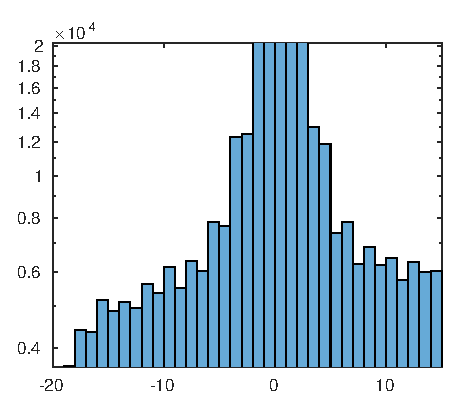
\includegraphics[width=5.5cm]{img/f3-hist.eps}
\caption{Part of a histogram of motion vectors with F3 embedding. Note the unusually higher peaks corresponding to even numbers.}
\label{fig:f3-hist}
\end{wrapfigure}

This leads to an interesting effect called \emph{shrinkage}. Whenever we try to embed a zero bit (\emph{steganographic zero}) into $mv_C = -1$ or $mv_C = 1$, the value of $mv_C$ will become 0, so the zero bit will have to be re-embedded again. It means that F3 will embed more steganographic zeroes than ones. 

This is the main weakness of the algorithm. Typical encrypted payload has the same number of steganographic zeroes and ones, but since F3 embedding will embed more zeros, values with LSB 0 will be more common (Figure \ref{fig:f3-hist}). However, the embedding is not vulnerable if steganographic ones are more common in the payload, so the shrinkage effect balances out the number of ones and zeroes embedded.  

\subsection{F4}

F4~\cite{f5} eliminates the weakness of F3 by using a different strategy for embedding into negative values of $mv_C$. Just like in F3, $mv_C$ is changed (if required) by decrementing its absolute value. Now when $mv_C$ is positive, the algorithm ensures its LSB matches that of the payload (just like F3), but when $mv_C$ is negative, algorithm ensures its LSB \emph{does not} match that of the payload. This mapping is visualised in Figure \ref{fig:f4-mapping} and the pseudocode is listed in Algorithm \ref{alg:f4-embed}.

\begin{algorithm}
\caption{Embedding procedure for \emph{F4}.}
\label{alg:f4-embed}
\begin{algorithmic}
\Procedure {F4-Embed}{$mv_C$, $payload_i$}
\If {$mv_C > 0$ \textbf{and} $\textit{LSB}(mv_C) \neq payload_i$}
    \State $mv_C \gets mv_C - 1$ \Comment {Decrease the absolute value of $mv_C$}
\EndIf
\If {$mv_C < 0$ \textbf{and} $\textit{LSB}(mv_C) = payload_i$}
	\State $mv_C \gets mv_C + 1$ \Comment {Decrease the absolute value of $mv_C$}
\EndIf

\State \Return $mv_C \neq 0$
\EndProcedure
\end{algorithmic}
\end{algorithm}

\begin{figure}[tbh]
\centering
\resizebox{0.75\textwidth}{!}{%LaTeX with PSTricks extensions
%%Creator: inkscape 0.91
%%Please note this file requires PSTricks extensions
\psset{xunit=.5pt,yunit=.5pt,runit=.5pt}
\begin{pspicture}(452.5,185)
{
\newrgbcolor{curcolor}{1 1 1}
\pscustom[linestyle=none,fillstyle=solid,fillcolor=curcolor]
{
\newpath
\moveto(0,185)
\lineto(452.5,185)
\lineto(452.5,0)
\lineto(0,0)
\lineto(0,185)
\closepath
}
}
{
\newrgbcolor{curcolor}{0 0 0}
\pscustom[linestyle=none,fillstyle=solid,fillcolor=curcolor]
{
\newpath
\moveto(4.46655275,170.5676275)
\curveto(4.6691895,170.30151375)(4.96582025,170.1684575)(5.35644525,170.1684575)
\curveto(6.15234375,170.1684575)(6.85791013,170.7690425)(7.4731445,171.970215)
\curveto(7.9956055,173.00048825)(8.25683588,173.94775387)(8.25683588,174.81201175)
\curveto(8.25683588,175.17822262)(8.21289062,175.47363287)(8.125,175.69824225)
\curveto(7.9541015,176.12304688)(7.6416015,176.33544925)(7.1875,176.33544925)
\curveto(6.44042963,176.33544925)(5.73974612,175.77636725)(5.08544925,174.65820312)
\curveto(4.47021487,173.61328125)(4.16259763,172.58544925)(4.16259763,171.5747075)
\curveto(4.16259763,171.16943375)(4.26391637,170.83374)(4.46655275,170.5676275)
\closepath
\moveto(9.00390625,175.98754887)
\curveto(9.34082025,175.55053713)(9.50927737,175.03417975)(9.50927737,174.43847662)
\curveto(9.50927737,173.40332037)(9.05273438,172.387695)(8.13964838,171.39160125)
\curveto(7.19726562,170.356445)(6.19140625,169.8388675)(5.12207025,169.8388675)
\curveto(4.44824225,169.8388675)(3.90869138,170.03418)(3.503418,170.424805)
\curveto(3.0981445,170.81543)(2.89550775,171.36474625)(2.89550775,172.07275375)
\curveto(2.89550775,173.14208988)(3.34960938,174.16503912)(4.2578125,175.14160162)
\curveto(5.18554688,176.14257812)(6.18896487,176.64306637)(7.26806638,176.64306637)
\curveto(8.08837888,176.64306637)(8.66699225,176.4245605)(9.00390625,175.98754887)
\closepath
\moveto(13.1457525,176.62475588)
\curveto(13.16284,176.59790087)(13.17139,176.56738337)(13.17139,176.53320337)
\curveto(13.166515,176.48437462)(13.16164,176.44775462)(13.15674,176.42333963)
\lineto(12.42431638,173.58886713)
\lineto(12.58544875,173.90380863)
\curveto(12.93701125,174.59228512)(13.34838875,175.22094725)(13.81958,175.78979488)
\curveto(14.29077125,176.35864262)(14.73877,176.64306637)(15.16357375,176.64306637)
\curveto(15.39306625,176.64306637)(15.57006875,176.56738262)(15.69458,176.41601562)
\curveto(15.8190925,176.2646485)(15.8813475,176.09130863)(15.8813475,175.89599613)
\curveto(15.8813475,175.6762695)(15.819085,175.49438475)(15.69458,175.35034175)
\curveto(15.5700675,175.20629888)(15.39794875,175.13427738)(15.1782225,175.13427738)
\curveto(15.026855,175.13427738)(14.91211,175.16357362)(14.833985,175.22216737)
\curveto(14.75586,175.28076112)(14.69482375,175.3491205)(14.65087875,175.4272455)
\lineto(14.56299125,175.58837825)
\curveto(14.54345375,175.6176745)(14.52026625,175.64086825)(14.49341625,175.65795825)
\curveto(14.46655375,175.67504825)(14.43360375,175.68359325)(14.39454125,175.68359325)
\curveto(14.20411125,175.68359325)(13.92945375,175.41748)(13.57056625,174.88525337)
\curveto(13.21167,174.35302738)(12.890625,173.7768555)(12.6074225,173.15673825)
\curveto(12.43652338,172.78076175)(12.24609375,172.282715)(12.03613287,171.6625975)
\curveto(11.90429688,171.2719725)(11.72851562,170.71777375)(11.50878912,170)
\lineto(10.38085938,170)
\lineto(11.59667963,174.40917963)
\curveto(11.66503963,174.66308588)(11.71997087,174.89013675)(11.76147462,175.090332)
\curveto(11.80297837,175.29052738)(11.82373087,175.45410162)(11.82373087,175.58105475)
\curveto(11.82373087,175.72753912)(11.78710962,175.83984375)(11.71386712,175.91796875)
\curveto(11.64062462,175.99609375)(11.51367175,176.03515625)(11.33300775,176.03515625)
\curveto(11.274414,176.03515625)(11.20117175,176.03026875)(11.11328112,176.0205075)
\curveto(11.02539112,176.010745)(10.92041,175.998535)(10.79833975,175.98388625)
\lineto(10.79833975,176.2255855)
\lineto(11.0913085,176.28417925)
\curveto(11.472168,176.36230475)(11.88842775,176.4453125)(12.34008788,176.53320312)
\curveto(12.7917475,176.62109375)(13.029785,176.66503912)(13.05419875,176.66503912)
\curveto(13.09814875,176.66503912)(13.12866125,176.65161162)(13.14574875,176.62475538)
\closepath
\moveto(18.53027375,178.47412113)
\curveto(18.3886725,178.63037113)(18.31787125,178.81835938)(18.31787125,179.038086)
\curveto(18.31787125,179.26269525)(18.38867125,179.453125)(18.53027375,179.609375)
\curveto(18.671875,179.765625)(18.84277375,179.84375)(19.04296875,179.84375)
\curveto(19.24316375,179.84375)(19.41528375,179.765625)(19.55932625,179.609375)
\curveto(19.70336875,179.453125)(19.77539125,179.26269525)(19.77539125,179.038086)
\curveto(19.77539125,178.8134765)(19.70336625,178.62426762)(19.55932625,178.470459)
\curveto(19.41528375,178.31665037)(19.24316375,178.23974613)(19.04296875,178.23974613)
\curveto(18.84277375,178.23974613)(18.671875,178.31787113)(18.53027375,178.47412113)
\closepath
\moveto(19.25537125,176.5771485)
\lineto(17.77587875,171.34765625)
\curveto(17.70751625,171.06933625)(17.67334125,170.90332)(17.67334125,170.84960875)
\curveto(17.67334125,170.77637125)(17.68799125,170.71289)(17.71729125,170.65918)
\curveto(17.74170375,170.6005925)(17.80274125,170.5712925)(17.9003975,170.5712925)
\curveto(18.0664125,170.5712925)(18.28613875,170.71533625)(18.55957625,171.00342125)
\curveto(18.72071,171.17432)(18.91846375,171.41846125)(19.15283875,171.73584375)
\lineto(19.3432675,171.57471125)
\lineto(19.27003,171.47217375)
\curveto(18.90381875,170.95947875)(18.60108375,170.59082625)(18.36182625,170.3662175)
\curveto(17.98585,170.014655)(17.61963875,169.83887375)(17.26319375,169.83887375)
\curveto(17.0532325,169.83887375)(16.8786725,169.92676125)(16.7395125,170.102545)
\curveto(16.60035125,170.27832625)(16.53077125,170.48584625)(16.53077125,170.72510375)
\curveto(16.53077125,170.866705)(16.54052125,170.98999625)(16.56007125,171.0949775)
\curveto(16.57960875,171.1999525)(16.61622125,171.35498625)(16.66993375,171.560065)
\lineto(17.6953125,175.324707)
\curveto(17.7099625,175.38330075)(17.7221625,175.437012)(17.7319375,175.48583988)
\curveto(17.7416875,175.53466862)(17.7465875,175.58349613)(17.7465875,175.63232425)
\curveto(17.7465875,175.8081055)(17.6818875,175.916748)(17.552495,175.958252)
\curveto(17.42310125,175.99975575)(17.16797375,176.02050825)(16.787115,176.02050825)
\lineto(16.787115,176.26220738)
\curveto(17.1923875,176.31103612)(17.48413625,176.34887738)(17.66235875,176.37573238)
\curveto(17.84058125,176.40258737)(18.020025,176.43066362)(18.20068875,176.45996113)
\curveto(18.43506375,176.49902363)(18.65723125,176.54296863)(18.8671925,176.591797)
\curveto(19.07715375,176.64062575)(19.19556125,176.6564945)(19.2224175,176.6394045)
\curveto(19.2492675,176.6223145)(19.260255,176.60156325)(19.25538,176.57714825)
\closepath
\moveto(22.71972625,173.02490238)
\curveto(22.87597625,172.72705075)(23.15673875,172.578125)(23.56201125,172.578125)
\curveto(24.001465,172.578125)(24.39331,172.857666)(24.73754875,173.416748)
\curveto(25.0817875,173.97583013)(25.25390625,174.59228512)(25.25390625,175.26611325)
\curveto(25.25390625,175.58837887)(25.18310625,175.8410645)(25.04150375,176.02416988)
\curveto(24.8999025,176.20727537)(24.6875,176.29882812)(24.40429625,176.29882812)
\curveto(23.85742125,176.29882812)(23.4167475,176.00830075)(23.082275,175.42724613)
\curveto(22.7478025,174.84619137)(22.58056625,174.28710938)(22.58056625,173.75)
\curveto(22.58056625,173.44726562)(22.62695375,173.20556637)(22.71972625,173.02490238)
\closepath
\moveto(24.2834475,167.6342775)
\curveto(24.6667475,167.9125975)(24.85839875,168.24462875)(24.85839875,168.63037125)
\curveto(24.85839875,168.92334)(24.75829875,169.16992125)(24.558105,169.3701175)
\curveto(24.45068,169.4775425)(24.27734375,169.592285)(24.03808625,169.714355)
\curveto(23.83789,169.8120175)(23.49975625,169.9523925)(23.02368125,170.1354975)
\curveto(22.5476075,170.31860375)(22.27294875,170.41015625)(22.1997075,170.41015625)
\curveto(22.07275375,170.41015625)(21.82617125,170.24047875)(21.45996125,169.9011225)
\curveto(21.09375,169.5617675)(20.910645,169.17724625)(20.910645,168.74755875)
\curveto(20.910645,168.098145)(21.19140625,167.6513675)(21.75293,167.40722625)
\curveto(22.04589875,167.28027375)(22.40722625,167.21679625)(22.83691375,167.21679625)
\curveto(23.41796875,167.21679625)(23.90014625,167.3559575)(24.2834475,167.6342775)
\closepath
\moveto(20.51879875,169.60083)
\curveto(20.79956,169.93042)(21.2451175,170.25878875)(21.85546875,170.5859375)
\curveto(21.73339375,170.6640625)(21.63330125,170.74585)(21.55517625,170.83129875)
\curveto(21.47705125,170.91674875)(21.43798875,171.03027375)(21.43798875,171.171875)
\curveto(21.43798875,171.37207)(21.57714875,171.6015625)(21.85546875,171.86035125)
\curveto(22.01171875,172.00683625)(22.265625,172.1997075)(22.6171875,172.438965)
\curveto(22.3046875,172.5561525)(22.0361325,172.722168)(21.81152375,172.93701175)
\curveto(21.53808625,173.22509762)(21.4013675,173.59863287)(21.4013675,174.05761713)
\curveto(21.4013675,174.79492188)(21.6894525,175.40771488)(22.265625,175.89599613)
\curveto(22.84179625,176.38427738)(23.5546875,176.628418)(24.40429625,176.628418)
\curveto(24.8486325,176.628418)(25.22460875,176.558838)(25.53222625,176.41967775)
\curveto(25.83984375,176.28051763)(26.0205075,176.16455075)(26.07421875,176.07177738)
\lineto(27.06298875,176.07177738)
\lineto(27.06298875,175.48583988)
\lineto(26.3159175,175.48583988)
\curveto(26.3452175,175.37841862)(26.3671925,175.28076175)(26.38183,175.19287113)
\curveto(26.39648,175.10498112)(26.403805,174.98046875)(26.403805,174.81933588)
\curveto(26.403805,174.02832037)(26.09740875,173.40576175)(25.484615,172.95166012)
\curveto(24.8718225,172.49755875)(24.2114225,172.2705075)(23.50341375,172.2705075)
\curveto(23.43017625,172.2705075)(23.3618125,172.2741325)(23.29833625,172.2815075)
\curveto(23.23486125,172.2888825)(23.156735,172.3022575)(23.06396125,172.321795)
\curveto(22.99072375,172.321795)(22.89062125,172.250995)(22.7636675,172.1093925)
\curveto(22.6318325,171.96779125)(22.56591375,171.8408375)(22.56591375,171.7285325)
\curveto(22.56591375,171.5625175)(23.10302375,171.27931375)(24.1772425,170.87892375)
\curveto(25.24657875,170.47365)(25.78124625,169.88038875)(25.78124625,169.09913875)
\curveto(25.78124625,168.51320125)(25.51269125,167.999285)(24.9755825,167.55739)
\curveto(24.4384725,167.11549625)(23.62792625,166.89454875)(22.54394125,166.89454875)
\curveto(21.79198875,166.89454875)(21.196285,167.05568125)(20.7568325,167.3779475)
\curveto(20.31737875,167.7002125)(20.0976525,168.09327875)(20.0976525,168.55714625)
\curveto(20.0976525,168.9233575)(20.23803375,169.2712575)(20.518795,169.6008475)
\closepath
\moveto(30.19043,178.47412113)
\curveto(30.0488275,178.63037113)(29.9780275,178.81835938)(29.9780275,179.038086)
\curveto(29.9780275,179.26269525)(30.0488275,179.453125)(30.19043,179.609375)
\curveto(30.33203125,179.765625)(30.50293,179.84375)(30.703125,179.84375)
\curveto(30.90332,179.84375)(31.07543875,179.765625)(31.2194825,179.609375)
\curveto(31.363525,179.453125)(31.43554625,179.26269525)(31.43554625,179.038086)
\curveto(31.43554625,178.8134765)(31.36352125,178.62426762)(31.2194825,178.470459)
\curveto(31.07543875,178.31665037)(30.90332,178.23974613)(30.703125,178.23974613)
\curveto(30.50293,178.23974613)(30.33203125,178.31787113)(30.19043,178.47412113)
\closepath
\moveto(30.9155275,176.5771485)
\lineto(29.436035,171.34765625)
\curveto(29.3676725,171.06933625)(29.3334975,170.90332)(29.3334975,170.84960875)
\curveto(29.3334975,170.77637125)(29.3481475,170.71289)(29.3774475,170.65918)
\curveto(29.40186,170.6005925)(29.4628975,170.5712925)(29.5605525,170.5712925)
\curveto(29.72656875,170.5712925)(29.946295,170.71533625)(30.2197325,171.00342125)
\curveto(30.380865,171.17432)(30.57862,171.41846125)(30.812995,171.73584375)
\lineto(31.00342375,171.57471125)
\lineto(30.93018625,171.47217375)
\curveto(30.563975,170.95947875)(30.26124,170.59082625)(30.0219825,170.3662175)
\curveto(29.64600625,170.014655)(29.279795,169.83887375)(28.92335,169.83887375)
\curveto(28.71338875,169.83887375)(28.53882875,169.92676125)(28.3996675,170.102545)
\curveto(28.2605075,170.27832625)(28.1909275,170.48584625)(28.1909275,170.72510375)
\curveto(28.1909275,170.866705)(28.2006775,170.98999625)(28.2202275,171.0949775)
\curveto(28.239765,171.1999525)(28.2763775,171.35498625)(28.33009,171.560065)
\lineto(29.35548125,175.32471325)
\curveto(29.37013125,175.383307)(29.38233125,175.43701825)(29.39210625,175.48584612)
\curveto(29.40185625,175.53467488)(29.40675625,175.58350237)(29.40675625,175.6323305)
\curveto(29.40675625,175.80811175)(29.34205625,175.91675425)(29.21266375,175.95825825)
\curveto(29.08326875,175.999762)(28.8281425,176.0205145)(28.4472825,176.0205145)
\lineto(28.4472825,176.26221363)
\curveto(28.85255625,176.31104237)(29.144305,176.34888363)(29.3225275,176.37573862)
\curveto(29.50075,176.40259363)(29.68019375,176.43066988)(29.8608575,176.45996737)
\curveto(30.0952325,176.49902987)(30.3174,176.54297487)(30.52736125,176.59180325)
\curveto(30.7373225,176.640632)(30.85573,176.65650075)(30.88258625,176.63941075)
\curveto(30.90943625,176.62232075)(30.92042375,176.6015695)(30.91554875,176.5771545)
\closepath
\moveto(31.91162125,170)
\lineto(33.17871125,174.52636713)
\curveto(33.28613625,174.90722662)(33.34838875,175.1379395)(33.36547875,175.21850588)
\curveto(33.38256625,175.29907213)(33.39111625,175.38574225)(33.39111625,175.47851562)
\curveto(33.39111625,175.62011725)(33.35082875,175.73120112)(33.27026625,175.81176762)
\curveto(33.18970375,175.89233387)(33.03222875,175.93261763)(32.79785375,175.93261763)
\curveto(32.73926625,175.93261763)(32.68189125,175.92895512)(32.625735,175.92163013)
\curveto(32.569585,175.91430512)(32.5073225,175.90576137)(32.4389675,175.89599513)
\lineto(32.4389675,176.1450185)
\curveto(32.75635,176.19384725)(32.98218,176.23046725)(33.1164575,176.25488225)
\curveto(33.250735,176.279296)(33.39599875,176.3085935)(33.55224875,176.3427735)
\lineto(34.86328375,176.628418)
\curveto(34.89258375,176.60888675)(34.91210875,176.58691425)(34.92187125,176.5625005)
\lineto(33.94775,173.41308638)
\curveto(34.54345375,174.32617237)(35.0415,175.00488325)(35.44189125,175.44921925)
\curveto(36.14501625,176.23535212)(36.77489875,176.6284185)(37.33153875,176.6284185)
\curveto(37.5463825,176.6284185)(37.73193,176.58691475)(37.88818,176.50390725)
\curveto(38.18603125,176.3427745)(38.3349575,176.05224713)(38.3349575,175.63232525)
\curveto(38.3349575,175.51513775)(38.3227075,175.39306737)(38.2983325,175.26611425)
\curveto(38.27392,175.13916112)(38.2421825,175.00244237)(38.20312,174.855958)
\lineto(37.2436475,171.3476575)
\curveto(37.22411,171.27442)(37.2021475,171.18530375)(37.177735,171.08032375)
\curveto(37.1533225,170.97533625)(37.14111,170.90088)(37.14111,170.856935)
\curveto(37.14111,170.7836975)(37.1581975,170.717775)(37.192385,170.65918125)
\curveto(37.22656,170.60059375)(37.2827225,170.57129375)(37.3608425,170.57129375)
\curveto(37.487795,170.57129375)(37.63428,170.64575625)(37.800295,170.7946825)
\curveto(37.96631125,170.94360875)(38.2373075,171.2622125)(38.61328375,171.75049375)
\lineto(38.82568625,171.56006375)
\curveto(38.425295,171.01807125)(38.1079125,170.6372125)(37.8735375,170.417485)
\curveto(37.4731475,170.03174375)(37.08984625,169.8388725)(36.723635,169.8388725)
\curveto(36.55762,169.8388725)(36.3977075,169.89381)(36.24389875,170.0036675)
\curveto(36.09009,170.11353)(36.01318625,170.312505)(36.01318625,170.60059125)
\curveto(36.01318625,170.68360375)(36.01931125,170.77148875)(36.03149875,170.8642625)
\curveto(36.04374875,170.9570375)(36.05957375,171.0376025)(36.07911125,171.1059625)
\lineto(37.0019625,174.66553212)
\curveto(37.0507875,174.86084462)(37.08375,175.02075675)(37.1008375,175.14526838)
\curveto(37.117925,175.26977963)(37.126475,175.3588915)(37.126475,175.41260238)
\curveto(37.126475,175.52978988)(37.0984,175.63110825)(37.04225,175.7165575)
\curveto(36.9861,175.80200625)(36.88722125,175.84473138)(36.74561875,175.84473138)
\curveto(36.37940875,175.84473138)(35.9179825,175.5127)(35.36134125,174.84863763)
\curveto(35.03418,174.453125)(34.70214875,173.98193363)(34.36523375,173.43505863)
\curveto(34.106445,173.01025387)(33.9025875,172.5964355)(33.7536625,172.19360375)
\curveto(33.60473625,171.79077125)(33.36914,171.05957)(33.046875,170)
\lineto(31.91162125,170)
\closepath
\moveto(44.3627925,176.06445312)
\curveto(44.20166,176.23046875)(44.0063475,176.3134765)(43.776855,176.3134765)
\curveto(42.9809575,176.3134765)(42.24121125,175.703125)(41.5576175,174.48242188)
\curveto(40.95703125,173.40820312)(40.65673875,172.48291)(40.65673875,171.7065425)
\curveto(40.65673875,171.3159175)(40.74096375,171.03149375)(40.90942375,170.85327125)
\curveto(41.07788125,170.67504875)(41.28662125,170.5859375)(41.535645,170.5859375)
\curveto(42.27294875,170.5859375)(42.98339875,171.17919875)(43.6669925,172.3657225)
\curveto(44.2919925,173.44482425)(44.6044925,174.41894525)(44.6044925,175.288086)
\curveto(44.6044925,175.6396485)(44.52393,175.8984375)(44.3627925,176.06445312)
\closepath
\moveto(44.58252,176.3427735)
\curveto(44.69482,176.23535225)(44.782715,176.09375)(44.84619125,175.91796875)
\lineto(44.88281625,175.81543)
\lineto(45.04394875,176.3720705)
\curveto(45.06348625,176.43554675)(45.08057375,176.47827175)(45.09522375,176.50024437)
\curveto(45.10987375,176.52221687)(45.14404875,176.53564438)(45.19776125,176.54052813)
\lineto(46.02539875,176.63574313)
\curveto(46.06934875,176.63574313)(46.09497375,176.62719312)(46.10229875,176.61010813)
\curveto(46.10967375,176.59301812)(46.10842375,176.56250062)(46.09867375,176.51855563)
\curveto(46.07913625,176.45507937)(46.06449875,176.40503062)(46.05472375,176.36840912)
\curveto(46.04497375,176.33178788)(46.03031125,176.27929787)(46.01077375,176.21093838)
\lineto(45.336945,173.588868)
\curveto(45.19046125,173.017579)(45.06594875,172.52441487)(44.96341,172.10937625)
\curveto(44.78274625,171.3574225)(44.69241375,170.927735)(44.69241375,170.82031375)
\curveto(44.69241375,170.75195125)(44.71072625,170.70190125)(44.74735125,170.6701675)
\curveto(44.78397625,170.63843)(44.82913875,170.622555)(44.88285,170.622555)
\curveto(44.9268,170.622555)(44.9744,170.637205)(45.0256725,170.666505)
\curveto(45.0769475,170.695805)(45.1391975,170.7397425)(45.21244,170.79834125)
\lineto(45.3369525,170.90087875)
\curveto(45.376015,170.93505375)(45.419965,170.97534125)(45.46878875,171.02172875)
\curveto(45.51761375,171.06811625)(45.57621375,171.12549125)(45.64457,171.1938475)
\lineto(46.09867125,171.6625975)
\lineto(46.2744525,171.50878875)
\curveto(45.76664,170.859375)(45.358925,170.41870125)(45.05130875,170.1867675)
\curveto(44.74369125,169.95483375)(44.4507225,169.8388675)(44.1724025,169.8388675)
\curveto(43.9917375,169.8388675)(43.8513575,169.9023425)(43.75125875,170.02929625)
\curveto(43.65115875,170.15625)(43.6011125,170.31494125)(43.6011125,170.50537125)
\curveto(43.6011125,170.6811525)(43.634075,170.9338375)(43.6999875,171.2634275)
\curveto(43.7659,171.5930175)(43.8306025,171.8701175)(43.89407875,172.09472625)
\curveto(43.80619125,171.9482425)(43.65848375,171.73461875)(43.45096375,171.4538575)
\curveto(43.24344375,171.17309625)(42.9883175,170.90087875)(42.6855825,170.6372075)
\curveto(42.3291375,170.31982375)(41.98734125,170.095215)(41.6601925,169.96337875)
\curveto(41.40628625,169.87549125)(41.162145,169.8315425)(40.92777,169.8315425)
\curveto(40.5322625,169.8315425)(40.17337625,169.99389625)(39.85111,170.31860375)
\curveto(39.528845,170.64331)(39.3677125,171.103515)(39.3677125,171.69921875)
\curveto(39.3677125,172.724609)(39.82669625,173.79394487)(40.744665,174.90722625)
\curveto(41.69193125,176.06445275)(42.67337625,176.643066)(43.68900125,176.643066)
\curveto(44.07474375,176.643066)(44.372595,176.5429685)(44.58255625,176.34277313)
\closepath
\moveto(49.36523375,178.88427738)
\curveto(49.38477125,178.94775362)(49.39697125,179.0112305)(49.40185875,179.074707)
\curveto(49.40673375,179.13818325)(49.40923375,179.18945325)(49.40923375,179.22851562)
\curveto(49.40923375,179.39453125)(49.34209625,179.49584963)(49.2078175,179.53247075)
\curveto(49.07354,179.569092)(48.80620625,179.58496075)(48.405815,179.58007825)
\lineto(48.405815,179.8217775)
\curveto(48.6255425,179.85107375)(48.8782275,179.88525375)(49.1638725,179.92431625)
\curveto(49.44951625,179.96337875)(49.63628375,179.99023375)(49.724175,180.0048825)
\curveto(49.9976125,180.05371125)(50.32964375,180.1269525)(50.72026875,180.22460913)
\curveto(50.75444375,180.22460913)(50.78863125,180.20019537)(50.82280625,180.15136663)
\lineto(48.515625,171.34765625)
\curveto(48.4619125,171.137695)(48.430175,171.0107425)(48.4204125,170.96679625)
\curveto(48.4106625,170.92284625)(48.4057625,170.87890875)(48.4057625,170.83496125)
\curveto(48.4057625,170.74218625)(48.42285,170.66284125)(48.4570375,170.59692375)
\curveto(48.4912125,170.53101125)(48.5547,170.49804875)(48.6474675,170.49804875)
\curveto(48.82324875,170.49804875)(49.05274,170.65429875)(49.33594375,170.96679875)
\curveto(49.6191475,171.27929875)(49.858405,171.58203375)(50.0537175,171.8750025)
\lineto(50.25147125,171.7358425)
\curveto(49.83154875,171.115725)(49.50440125,170.6860375)(49.27002625,170.44678)
\curveto(48.8647525,170.04150625)(48.4570375,169.83887)(48.04688125,169.83887)
\curveto(47.8711,169.83887)(47.71485,169.88282)(47.57813125,169.970705)
\curveto(47.36817,170.10254125)(47.26319,170.32715125)(47.26319,170.64453375)
\curveto(47.26319,170.76660875)(47.2827275,170.93017875)(47.3217775,171.13525625)
\curveto(47.34619,171.25733125)(47.3779275,171.39892875)(47.41699,171.56006125)
\lineto(49.36523125,178.88427988)
\closepath
\moveto(60.71777375,176.32080075)
\curveto(60.8642575,176.12548825)(60.9375,175.90332025)(60.9375,175.65429688)
\curveto(60.9375,174.99511713)(60.285645,173.840332)(58.98193375,172.18994125)
\curveto(57.7465825,170.62255875)(57.00683625,169.8388675)(56.762695,169.8388675)
\curveto(56.6894575,169.8388675)(56.64062,169.9389675)(56.61621125,170.13916)
\curveto(56.60156125,170.25146)(56.59423625,170.441895)(56.59423625,170.71044875)
\curveto(56.59423625,171.0375975)(56.56249875,171.59179625)(56.49902375,172.37304625)
\curveto(56.43554625,173.15429688)(56.37451125,173.73291012)(56.3159175,174.10888675)
\curveto(56.1938475,174.934082)(56.07421875,175.46630863)(55.95703125,175.70556637)
\curveto(55.83984375,175.94482425)(55.61767625,176.06445312)(55.2905275,176.06445312)
\curveto(55.236815,176.06445312)(55.174565,176.06201563)(55.10376,176.05712812)
\curveto(55.03296,176.05224062)(54.95117125,176.04491562)(54.85839875,176.03515562)
\lineto(54.85839875,176.22558538)
\curveto(55.0048825,176.25488275)(55.3125,176.32080075)(55.78125,176.42333988)
\curveto(56.25,176.52587887)(56.49902375,176.58203125)(56.52832,176.59179688)
\lineto(56.77002,176.66503937)
\curveto(56.8383825,176.68457062)(56.892095,176.64672938)(56.9311525,176.55151438)
\curveto(56.970215,176.45629938)(57.01904,176.27929762)(57.07763625,176.02050862)
\curveto(57.26318375,175.17089925)(57.40234375,174.33349688)(57.4951175,173.5083015)
\curveto(57.553705,172.99560625)(57.612305,172.23632875)(57.67089875,171.23047)
\lineto(57.9125975,171.4868175)
\curveto(58.4155275,172.01904375)(58.9184575,172.65136788)(59.42138625,173.38378987)
\curveto(59.92431625,174.11621163)(60.17578125,174.63378987)(60.17578125,174.93652413)
\curveto(60.17578125,175.08789137)(60.06591875,175.26977612)(59.84619125,175.4821785)
\curveto(59.626465,175.69458088)(59.51660125,175.88867262)(59.51660125,176.06445387)
\curveto(59.51660125,176.22558675)(59.57153875,176.35742262)(59.68139625,176.45996175)
\curveto(59.79125875,176.5625005)(59.9267575,176.61377025)(60.08789125,176.61377025)
\curveto(60.3613275,176.61377025)(60.57128875,176.516114)(60.71777375,176.3208015)
\closepath
\moveto(66.41357375,176.06445312)
\curveto(66.25244125,176.23046875)(66.05712875,176.3134765)(65.82763625,176.3134765)
\curveto(65.03173875,176.3134765)(64.2919925,175.703125)(63.60839875,174.48242188)
\curveto(63.0078125,173.40820312)(62.70752,172.48291)(62.70752,171.7065425)
\curveto(62.70752,171.3159175)(62.791745,171.03149375)(62.960205,170.85327125)
\curveto(63.1286625,170.67504875)(63.3374025,170.5859375)(63.58642625,170.5859375)
\curveto(64.32373,170.5859375)(65.03418,171.17919875)(65.71777375,172.3657225)
\curveto(66.34277375,173.44482425)(66.65527375,174.41894525)(66.65527375,175.288086)
\curveto(66.65527375,175.6396485)(66.57471125,175.8984375)(66.41357375,176.06445312)
\closepath
\moveto(66.63330125,176.3427735)
\curveto(66.74560125,176.23535225)(66.83349625,176.09375)(66.8969725,175.91796875)
\lineto(66.9335975,175.81543)
\lineto(67.09473,176.3720705)
\curveto(67.1142675,176.43554675)(67.131355,176.47827175)(67.146005,176.50024437)
\curveto(67.160655,176.52221687)(67.19483,176.53564438)(67.2485425,176.54052813)
\lineto(68.07617875,176.63574313)
\curveto(68.12012875,176.63574313)(68.14575375,176.62719312)(68.15307875,176.61010813)
\curveto(68.16045375,176.59301812)(68.15920375,176.56250062)(68.14945375,176.51855563)
\curveto(68.12991625,176.45507937)(68.11527875,176.40503062)(68.10550375,176.36840912)
\curveto(68.09575375,176.33178788)(68.08109125,176.27929787)(68.06155375,176.21093838)
\lineto(67.387725,173.588868)
\curveto(67.24124125,173.017579)(67.11672875,172.52441487)(67.01419,172.10937625)
\curveto(66.83352625,171.3574225)(66.74319375,170.927735)(66.74319375,170.82031375)
\curveto(66.74319375,170.75195125)(66.76150625,170.70190125)(66.79813125,170.6701675)
\curveto(66.83475625,170.63843)(66.87991875,170.622555)(66.93363,170.622555)
\curveto(66.97758,170.622555)(67.02518,170.637205)(67.0764525,170.666505)
\curveto(67.1277275,170.695805)(67.1899775,170.7397425)(67.26322,170.79834125)
\lineto(67.3877325,170.90087875)
\curveto(67.426795,170.93505375)(67.470745,170.97534125)(67.51956875,171.02172875)
\curveto(67.56839375,171.06811625)(67.62699375,171.12549125)(67.69535,171.1938475)
\lineto(68.14945125,171.6625975)
\lineto(68.3252325,171.50878875)
\curveto(67.81742,170.859375)(67.409705,170.41870125)(67.10208875,170.1867675)
\curveto(66.79447125,169.95483375)(66.5015025,169.8388675)(66.2231825,169.8388675)
\curveto(66.0425175,169.8388675)(65.9021375,169.9023425)(65.80203875,170.02929625)
\curveto(65.70193875,170.15625)(65.6518925,170.31494125)(65.6518925,170.50537125)
\curveto(65.6518925,170.6811525)(65.684855,170.9338375)(65.7507675,171.2634275)
\curveto(65.81668,171.5930175)(65.8813825,171.8701175)(65.94485875,172.09472625)
\curveto(65.85697125,171.9482425)(65.70926375,171.73461875)(65.50174375,171.4538575)
\curveto(65.294225,171.17309625)(65.0390975,170.90087875)(64.7363625,170.6372075)
\curveto(64.3799175,170.31982375)(64.03812125,170.095215)(63.7109725,169.96337875)
\curveto(63.45706625,169.87549125)(63.21292625,169.8315425)(62.97855,169.8315425)
\curveto(62.5830425,169.8315425)(62.22415625,169.99389625)(61.90189,170.31860375)
\curveto(61.579625,170.64331)(61.4184925,171.103515)(61.4184925,171.69921875)
\curveto(61.4184925,172.724609)(61.87747625,173.79394487)(62.795445,174.90722625)
\curveto(63.74271125,176.06445275)(64.72415625,176.643066)(65.73978125,176.643066)
\curveto(66.12552375,176.643066)(66.423375,176.5429685)(66.63333625,176.34277313)
\closepath
\moveto(71.41601625,178.88427738)
\curveto(71.43554125,178.94775362)(71.44775375,179.0112305)(71.45264125,179.074707)
\curveto(71.45751625,179.13818325)(71.46001625,179.18945325)(71.46001625,179.22851562)
\curveto(71.46001625,179.39453125)(71.39287875,179.49584963)(71.2586,179.53247075)
\curveto(71.1243225,179.569092)(70.85698875,179.58496075)(70.4565975,179.58007825)
\lineto(70.4565975,179.8217775)
\curveto(70.676325,179.85107375)(70.92901,179.88525375)(71.214655,179.92431625)
\curveto(71.50029875,179.96337875)(71.68706625,179.99023375)(71.7749575,180.0048825)
\curveto(72.048395,180.05371125)(72.38042625,180.1269525)(72.77105125,180.22460913)
\curveto(72.80522625,180.22460913)(72.83941375,180.20019537)(72.87358875,180.15136663)
\lineto(70.56646,171.34765625)
\curveto(70.5127475,171.137695)(70.48101,171.0107425)(70.4712475,170.96679625)
\curveto(70.4614975,170.92284625)(70.4565975,170.87890875)(70.4565975,170.83496125)
\curveto(70.4565975,170.74218625)(70.473685,170.66284125)(70.5078725,170.59692375)
\curveto(70.5420475,170.53101125)(70.605535,170.49804875)(70.6983025,170.49804875)
\curveto(70.87408375,170.49804875)(71.103575,170.65429875)(71.38677875,170.96679875)
\curveto(71.66998125,171.27929875)(71.90924,171.58203375)(72.1045525,171.8750025)
\lineto(72.30230625,171.7358425)
\curveto(71.88238375,171.115725)(71.55523625,170.6860375)(71.32086125,170.44678)
\curveto(70.9155875,170.04150625)(70.5078725,169.83887)(70.09771625,169.83887)
\curveto(69.921935,169.83887)(69.765685,169.88282)(69.62896625,169.970705)
\curveto(69.419005,170.10254125)(69.314025,170.32715125)(69.314025,170.64453375)
\curveto(69.314025,170.76660875)(69.3335625,170.93017875)(69.3726125,171.13525625)
\curveto(69.397025,171.25733125)(69.4287625,171.39892875)(69.467825,171.56006125)
\lineto(71.4160675,178.88427938)
\closepath
\moveto(74.56543,175.288086)
\curveto(74.57518,175.3369135)(74.5837425,175.38207975)(74.5910675,175.423584)
\curveto(74.5984425,175.46508775)(74.6020675,175.50781275)(74.6020675,175.55175787)
\curveto(74.6020675,175.76171875)(74.5398175,175.88989262)(74.41529875,175.93627925)
\curveto(74.29078625,175.9826655)(74.05763375,176.00585925)(73.71583625,176.00585925)
\lineto(73.71583625,176.21093738)
\lineto(74.79249625,176.42333975)
\lineto(75.9570475,176.64306625)
\curveto(75.98146,176.64795375)(76.003435,176.63817875)(76.02296,176.61377)
\curveto(76.0424975,176.58935625)(76.04981,176.56494125)(76.044935,176.5405275)
\lineto(76.02296,176.43798875)
\lineto(74.72657375,171.45752)
\curveto(74.69239875,171.335445)(74.66798625,171.24023375)(74.65333625,171.171875)
\curveto(74.63868625,171.1035125)(74.63136125,171.0546875)(74.63136125,171.02539)
\curveto(74.63136125,170.91309)(74.66309875,170.825195)(74.72657375,170.76171875)
\curveto(74.79004875,170.69824375)(74.8730575,170.66650625)(74.9755975,170.66650625)
\curveto(75.2636825,170.66650625)(75.62379,170.92285375)(76.05591875,171.43554875)
\curveto(76.48804875,171.948245)(76.87257,172.48047125)(77.20948375,173.03222963)
\curveto(77.51221875,173.52539362)(77.79053875,174.07471)(78.044445,174.68017875)
\curveto(78.200695,175.05615538)(78.42530375,175.65429987)(78.7182725,176.47461237)
\lineto(79.82423,176.47461237)
\lineto(78.4399525,171.28174125)
\curveto(78.41554,171.18407875)(78.393565,171.0937525)(78.37404,171.010745)
\curveto(78.3545025,170.9277325)(78.34474,170.8593775)(78.34474,170.80566625)
\curveto(78.34474,170.74219125)(78.35939,170.68725375)(78.38869,170.64087125)
\curveto(78.41799,170.59448375)(78.4692525,170.57129625)(78.54249875,170.57129625)
\curveto(78.61573625,170.57129625)(78.691425,170.59937125)(78.76955,170.65552125)
\curveto(78.847675,170.71167125)(78.94533125,170.79834375)(79.06251875,170.91553125)
\curveto(79.11623125,170.96924375)(79.21388625,171.0839875)(79.3554875,171.25976875)
\curveto(79.443375,171.36719375)(79.577655,171.530765)(79.75832,171.7504925)
\lineto(79.9633975,171.61133125)
\curveto(79.73878875,171.2402375)(79.50441375,170.92041375)(79.2602725,170.65185875)
\curveto(78.77687375,170.1098675)(78.327655,169.83887125)(77.91261625,169.83887125)
\curveto(77.6977725,169.83887125)(77.52199125,169.89745875)(77.3852725,170.0146525)
\curveto(77.24855375,170.13184)(77.180195,170.314945)(77.180195,170.56396875)
\curveto(77.180195,170.69092125)(77.192445,170.83008125)(77.21682,170.98144875)
\curveto(77.2412325,171.13281625)(77.280295,171.303715)(77.3340075,171.49414375)
\curveto(77.421895,171.83594125)(77.53420375,172.2631875)(77.6709225,172.77588313)
\lineto(77.832055,173.39844175)
\lineto(77.78078,173.39844175)
\curveto(77.1069525,172.2802775)(76.5771675,171.48926125)(76.191425,171.02539375)
\curveto(75.52248,170.22949625)(74.890155,169.83154625)(74.2944525,169.83154625)
\curveto(74.13332,169.83154625)(73.986835,169.86572125)(73.85499875,169.93408375)
\curveto(73.6010925,170.0708025)(73.47414,170.3149425)(73.47414,170.666505)
\curveto(73.47414,170.7690425)(73.479015,170.8520525)(73.48879,170.91552875)
\curveto(73.49854,170.97900375)(73.51564,171.06689625)(73.540065,171.1792)
\lineto(74.56545625,175.28808775)
\closepath
\moveto(82.28515625,175.090332)
\curveto(83.2519525,176.105957)(84.25048875,176.6137695)(85.28076125,176.6137695)
\curveto(85.66162125,176.6137695)(85.964355,176.5258795)(86.188965,176.35009762)
\curveto(86.41357375,176.17431637)(86.52587875,175.913086)(86.52587875,175.56640625)
\curveto(86.52587875,174.86328125)(86.1145025,174.26147463)(85.2917475,173.76098638)
\curveto(84.46899375,173.260498)(83.603515,172.95410162)(82.6953125,172.84179688)
\lineto(82.2778325,172.79052688)
\curveto(82.2143575,172.5903315)(82.1704075,172.43042)(82.14599625,172.31079125)
\curveto(82.12158375,172.19116625)(82.10937125,172.041015)(82.10937125,171.86035125)
\curveto(82.10937125,171.43066375)(82.2497525,171.09619125)(82.53051375,170.85693375)
\curveto(82.811275,170.61767625)(83.1445275,170.49804625)(83.53027,170.49804625)
\curveto(83.89648,170.49804625)(84.28466375,170.62012125)(84.69482,170.8642575)
\curveto(84.929195,171.00585875)(85.26855125,171.259765)(85.71288625,171.62597625)
\lineto(85.90331625,171.45752)
\curveto(85.68359,171.17919875)(85.36864875,170.893555)(84.9584925,170.60058625)
\curveto(84.23095375,170.078125)(83.5009725,169.816895)(82.76855125,169.816895)
\curveto(82.2509725,169.816895)(81.79687125,170)(81.40624625,170.36621125)
\curveto(81.01562125,170.73242125)(80.82030875,171.25732375)(80.82030875,171.9409175)
\curveto(80.82030875,173.02490188)(81.30859,174.0747065)(82.2851525,175.0903315)
\closepath
\moveto(84.6582025,174.10522463)
\curveto(85.24414,174.62524412)(85.53710875,175.14160162)(85.53710875,175.65429688)
\curveto(85.53710875,175.83984375)(85.49315875,175.98754888)(85.40527375,176.09741213)
\curveto(85.31738625,176.20727587)(85.18798875,176.262207)(85.01709,176.262207)
\curveto(84.6997075,176.262207)(84.3884275,176.126709)(84.0832525,175.85571287)
\curveto(83.77807625,175.58471675)(83.5034175,175.27832025)(83.2592775,174.93652338)
\curveto(83.00048875,174.53613275)(82.79541,174.152832)(82.6440425,173.78662113)
\curveto(82.56103,173.59130863)(82.473145,173.36914062)(82.38037125,173.12011713)
\curveto(83.31298875,173.25683588)(84.072265,173.58520513)(84.6582025,174.10522463)
\closepath
}
}
{
\newrgbcolor{curcolor}{0 0 0}
\pscustom[linestyle=none,fillstyle=solid,fillcolor=curcolor]
{
\newpath
\moveto(8.66699225,18.8208)
\curveto(8.8134765,18.6254875)(8.88671875,18.403325)(8.88671875,18.1543)
\curveto(8.88671875,17.4951125)(8.23486325,16.3403375)(6.93115237,14.6899375)
\curveto(5.69580075,13.1225625)(4.95605475,12.3388625)(4.71191413,12.3388625)
\curveto(4.63867163,12.3388625)(4.58984413,12.4389875)(4.56542975,12.6391625)
\curveto(4.550781,12.7514125)(4.54345725,12.9419)(4.54345725,13.21045)
\curveto(4.54345725,13.5376)(4.5117185,14.0918)(4.44824225,14.87305)
\curveto(4.384766,15.6543)(4.323731,16.2329125)(4.26513675,16.6088875)
\curveto(4.14306638,17.4340875)(4.0234375,17.9663125)(3.90625,18.2055625)
\curveto(3.7890625,18.444825)(3.5668945,18.56445)(3.23974612,18.56445)
\curveto(3.18603487,18.56445)(3.12377988,18.56195)(3.0529785,18.55695)
\curveto(2.98217725,18.55195)(2.90039062,18.54445)(2.80761725,18.53495)
\lineto(2.80761725,18.725375)
\curveto(2.95410162,18.754625)(3.26171875,18.820625)(3.73046875,18.923125)
\curveto(4.19921875,19.025625)(4.44824225,19.081825)(4.47753912,19.0915875)
\lineto(4.71923825,19.1648375)
\curveto(4.787597,19.1843375)(4.84130825,19.1465875)(4.88037112,19.0513375)
\curveto(4.91943362,18.9560875)(4.96826112,18.779125)(5.0268555,18.5203375)
\curveto(5.21240237,17.670725)(5.3515625,16.833325)(5.44433588,16.008125)
\curveto(5.50292963,15.4954375)(5.56152338,14.73615)(5.62011725,13.7303)
\lineto(5.86181638,13.9866375)
\curveto(6.36474612,14.518875)(6.86767575,15.1511875)(7.3706055,15.8836125)
\curveto(7.87353513,16.6160375)(8.125,17.1336125)(8.125,17.43635)
\curveto(8.125,17.5877125)(8.01513625,17.7696)(7.79541013,17.982)
\curveto(7.57568362,18.1944125)(7.46582025,18.3885)(7.46582025,18.564275)
\curveto(7.46582025,18.7254125)(7.5207515,18.85725)(7.63061525,18.9597875)
\curveto(7.740479,19.0622875)(7.8759765,19.1136)(8.03710937,19.1136)
\curveto(8.31054687,19.1136)(8.52050775,19.015975)(8.66699225,18.820625)
\closepath
\moveto(14.3627925,18.56445)
\curveto(14.20166,18.730475)(14.0063475,18.813475)(13.776855,18.813475)
\curveto(12.9809575,18.813475)(12.24121088,18.203125)(11.55761713,16.982425)
\curveto(10.95703125,15.9082)(10.65673825,14.9829125)(10.65673825,14.20655)
\curveto(10.65673825,13.815925)(10.740967,13.5315)(10.90942388,13.353275)
\curveto(11.07788088,13.17505)(11.28662113,13.0859375)(11.5356445,13.0859375)
\curveto(12.27294925,13.0859375)(12.98339875,13.6792)(13.6669925,14.865725)
\curveto(14.2919925,15.944825)(14.6044925,16.91895)(14.6044925,17.7880875)
\curveto(14.6044925,18.13965)(14.52393,18.3984375)(14.3627925,18.56445)
\closepath
\moveto(14.58252,18.842775)
\curveto(14.69482,18.7354)(14.782715,18.59375)(14.84619125,18.417975)
\lineto(14.88281625,18.315475)
\lineto(15.04394875,18.872125)
\curveto(15.06348625,18.935625)(15.08057375,18.978375)(15.09522375,19.0003)
\curveto(15.10987375,19.0223)(15.14404875,19.035675)(15.19776125,19.04055)
\lineto(16.02539875,19.1358)
\curveto(16.06934875,19.1358)(16.09497375,19.12705)(16.10229875,19.110175)
\curveto(16.10967375,19.09305)(16.10842375,19.06255)(16.09867375,19.01855)
\curveto(16.07913625,18.95505)(16.06449875,18.90505)(16.05472375,18.8684125)
\curveto(16.04497375,18.8317875)(16.03031125,18.7792875)(16.01077375,18.7109375)
\lineto(15.336945,16.0888625)
\curveto(15.19046125,15.517575)(15.06594875,15.0244125)(14.96341,14.609375)
\curveto(14.78274625,13.857425)(14.69241375,13.4277375)(14.69241375,13.3203125)
\curveto(14.69241375,13.2519375)(14.71072625,13.2019375)(14.74733875,13.1701625)
\curveto(14.78396375,13.1384125)(14.82912625,13.1225375)(14.8828375,13.1225375)
\curveto(14.9267875,13.1225375)(14.9743875,13.1371625)(15.02566,13.1664125)
\curveto(15.0769225,13.1956625)(15.139185,13.2396625)(15.2124275,13.29825)
\lineto(15.33694,13.40075)
\curveto(15.3760025,13.435)(15.4199525,13.47525)(15.46877625,13.521625)
\curveto(15.51760125,13.568)(15.57620125,13.625375)(15.6445575,13.69375)
\lineto(16.09865875,14.1625)
\lineto(16.27444,14.0086875)
\curveto(15.7666275,13.359275)(15.3589125,12.9186)(15.05129625,12.686675)
\curveto(14.74367875,12.4547375)(14.45071,12.3387625)(14.17239,12.3387625)
\curveto(13.991725,12.3387625)(13.851345,12.4022625)(13.7512475,12.5292)
\curveto(13.6511475,12.65615)(13.6011,12.8148375)(13.6011,13.005275)
\curveto(13.6011,13.18105)(13.6340625,13.4337375)(13.699975,13.763325)
\curveto(13.7658875,14.092925)(13.83059,14.3700125)(13.89406625,14.594625)
\curveto(13.80617875,14.4481375)(13.65847125,14.234525)(13.45095125,13.9537625)
\curveto(13.2434325,13.673)(12.988305,13.400775)(12.68557125,13.1371125)
\curveto(12.32912537,12.819725)(11.9873285,12.5951125)(11.66018,12.463275)
\curveto(11.40627375,12.3754)(11.16213312,12.33145)(10.92775812,12.33145)
\curveto(10.53225037,12.33145)(10.17336362,12.4938)(9.851098,12.8185)
\curveto(9.52883237,13.1432125)(9.3676995,13.6034125)(9.3676995,14.199125)
\curveto(9.3676995,15.2245125)(9.82668387,16.29385)(10.74465263,17.407125)
\curveto(11.69191825,18.56435)(12.67336375,19.1429625)(13.68898875,19.1429625)
\curveto(14.07473125,19.1429625)(14.3725825,19.0428375)(14.58254375,18.842675)
\closepath
\moveto(19.365235,21.384275)
\curveto(19.3847725,21.447775)(19.3969725,21.5112375)(19.40186,21.5747125)
\curveto(19.406735,21.6382125)(19.409235,21.6894625)(19.409235,21.7285125)
\curveto(19.409235,21.8945375)(19.3420975,21.99585)(19.20781875,22.032475)
\curveto(19.07354125,22.0691)(18.8062075,22.084975)(18.40581625,22.0801)
\lineto(18.40581625,22.3218)
\curveto(18.62554375,22.35105)(18.87822875,22.3853)(19.16387375,22.4243)
\curveto(19.4495175,22.4633)(19.636285,22.490175)(19.72417625,22.504925)
\curveto(19.99761375,22.5538)(20.329645,22.62705)(20.72027,22.72465)
\curveto(20.754445,22.72465)(20.7886325,22.700275)(20.8228075,22.6514)
\lineto(18.51567875,13.8477)
\curveto(18.46196625,13.6377375)(18.43022875,13.510775)(18.42046625,13.4668375)
\curveto(18.41071625,13.4228375)(18.40581625,13.3789625)(18.40581625,13.335)
\curveto(18.40581625,13.24225)(18.42290375,13.162875)(18.45709125,13.0969625)
\curveto(18.49126625,13.0310875)(18.55475375,12.9980875)(18.64752125,12.9980875)
\curveto(18.8233025,12.9980875)(19.052795,13.1543375)(19.3359975,13.4668375)
\curveto(19.61920125,13.7793375)(19.85845875,14.082075)(20.05377125,14.3750375)
\lineto(20.251525,14.235875)
\curveto(19.8316025,13.6157625)(19.504455,13.186075)(19.27008,12.9468125)
\curveto(18.86480625,12.5415375)(18.45709125,12.3389)(18.046935,12.3389)
\curveto(17.87115375,12.3389)(17.71490375,12.3829)(17.578185,12.4707375)
\curveto(17.36822375,12.602575)(17.26324375,12.8271875)(17.26324375,13.144575)
\curveto(17.26324375,13.2667)(17.28278125,13.4302125)(17.32183125,13.6352875)
\curveto(17.34624375,13.7574125)(17.37798125,13.8989625)(17.41704375,14.0601)
\lineto(19.36528625,21.3843125)
\closepath
\moveto(22.51464875,17.7880875)
\curveto(22.52439875,17.8369625)(22.53296125,17.8820875)(22.54028625,17.9235875)
\curveto(22.54766125,17.9650875)(22.55128625,18.0078375)(22.55128625,18.0517625)
\curveto(22.55128625,18.261725)(22.48903625,18.3899)(22.3645175,18.436275)
\curveto(22.240005,18.48265)(22.0068525,18.5059)(21.665055,18.5059)
\lineto(21.665055,18.710975)
\lineto(22.741715,18.923375)
\lineto(23.90626625,19.1431)
\curveto(23.93067875,19.1481)(23.95265375,19.1381)(23.97217875,19.11385)
\curveto(23.99171625,19.089475)(23.99902875,19.064975)(23.99415375,19.0406)
\lineto(23.97217875,18.9381)
\lineto(22.6757925,13.9576375)
\curveto(22.6416175,13.8355125)(22.617205,13.74035)(22.602555,13.6719875)
\curveto(22.587905,13.6036125)(22.58058,13.5548625)(22.58058,13.5255)
\curveto(22.58058,13.41325)(22.6123175,13.3253125)(22.6757925,13.2618375)
\curveto(22.7392675,13.1983375)(22.82227625,13.1665875)(22.92481625,13.1665875)
\curveto(23.21290125,13.1665875)(23.57300875,13.4229375)(24.0051375,13.9356375)
\curveto(24.4372675,14.448325)(24.82178875,14.9805625)(25.1587025,15.5323125)
\curveto(25.4614375,16.025475)(25.7397575,16.5748)(25.99366375,17.1802625)
\curveto(26.14991375,17.5562375)(26.3745225,18.1543875)(26.66749125,18.9747)
\lineto(27.77344875,18.9747)
\lineto(26.38917125,13.781825)
\curveto(26.36475875,13.6842)(26.34278375,13.5938375)(26.32325875,13.510825)
\curveto(26.30372125,13.427825)(26.29395875,13.3594625)(26.29395875,13.30575)
\curveto(26.29395875,13.24225)(26.30860875,13.187375)(26.33790875,13.1409625)
\curveto(26.36720875,13.0945875)(26.41847125,13.0713375)(26.4917175,13.0713375)
\curveto(26.564955,13.0713375)(26.64064375,13.0994625)(26.71876875,13.1555875)
\curveto(26.79689375,13.2117125)(26.89455,13.2984)(27.0117375,13.4155875)
\curveto(27.06545,13.4693375)(27.163105,13.58405)(27.30470625,13.759825)
\curveto(27.39259375,13.8672)(27.52687375,14.030825)(27.70753875,14.25055)
\lineto(27.91261625,14.1113875)
\curveto(27.6880075,13.7403)(27.4536325,13.420475)(27.20949125,13.151925)
\curveto(26.7260925,12.609925)(26.27687375,12.338925)(25.861835,12.338925)
\curveto(25.64699125,12.338925)(25.47121,12.39755)(25.33449125,12.5147125)
\curveto(25.1977725,12.6318375)(25.12941375,12.815)(25.12941375,13.064025)
\curveto(25.12941375,13.1909875)(25.14166375,13.3301375)(25.16603875,13.4815125)
\curveto(25.19045125,13.632875)(25.22951375,13.803775)(25.28322625,13.9942)
\curveto(25.37111375,14.336)(25.4834225,14.76325)(25.62014125,15.2759375)
\lineto(25.78127375,15.8985)
\lineto(25.72999875,15.8985)
\curveto(25.05617125,14.7803375)(24.52638625,13.989325)(24.14064375,13.52545)
\curveto(23.47169875,12.72955)(22.83937375,12.3316125)(22.24367125,12.3316125)
\curveto(22.08253875,12.3316125)(21.93605375,12.3657375)(21.8042175,12.4341125)
\curveto(21.55031125,12.570825)(21.42335875,12.8149625)(21.42335875,13.166525)
\curveto(21.42335875,13.269025)(21.42823375,13.352075)(21.43800875,13.41555)
\curveto(21.44775875,13.47905)(21.46485875,13.566925)(21.48928375,13.679225)
\lineto(22.514675,17.7881125)
\closepath
\moveto(30.234375,17.5903375)
\curveto(31.20117125,18.6059625)(32.1997075,19.113775)(33.22998,19.113775)
\curveto(33.61084,19.113775)(33.91357375,19.0259)(34.13818375,18.8501)
\curveto(34.3627925,18.6743125)(34.4750975,18.4130875)(34.4750975,18.0664125)
\curveto(34.4750975,17.3632875)(34.06372,16.761475)(33.24096625,16.2609875)
\curveto(32.4182125,15.7605)(31.55273375,15.4541)(30.64453125,15.3418)
\lineto(30.22705125,15.29055)
\curveto(30.16357625,15.0903625)(30.11962625,14.93045)(30.095215,14.8108125)
\curveto(30.0708025,14.6911875)(30.05859,14.5410375)(30.05859,14.360375)
\curveto(30.05859,13.9306875)(30.19897125,13.5962125)(30.4797325,13.3569625)
\curveto(30.76049375,13.1177)(31.09374625,12.998075)(31.47948875,12.998075)
\curveto(31.84569875,12.998075)(32.2338825,13.1202)(32.64403875,13.3642875)
\curveto(32.87841375,13.5058875)(33.21777,13.7597875)(33.662105,14.126)
\lineto(33.852535,13.95755)
\curveto(33.63280875,13.679225)(33.3178675,13.393575)(32.90771125,13.1006125)
\curveto(32.1801725,12.57815)(31.45019125,12.316925)(30.71777,12.316925)
\curveto(30.20019125,12.316925)(29.74609,12.500025)(29.355465,12.8662375)
\curveto(28.96484,13.23245)(28.7695275,13.75735)(28.7695275,14.44095)
\curveto(28.7695275,15.524925)(29.25780875,16.5747375)(30.23437125,17.5903625)
\closepath
\moveto(32.60742125,16.605225)
\curveto(33.19335875,17.12525)(33.4863275,17.6416)(33.4863275,18.1543)
\curveto(33.4863275,18.3398375)(33.4423775,18.48755)(33.3544925,18.5974125)
\curveto(33.266605,18.7072875)(33.1372075,18.7622125)(32.96630875,18.7622125)
\curveto(32.64892625,18.7622125)(32.33764625,18.6267125)(32.03247,18.3557125)
\curveto(31.727295,18.0847125)(31.45263625,17.778325)(31.20849625,17.436525)
\curveto(30.9497075,17.0361375)(30.74462875,16.6528375)(30.59326125,16.286625)
\curveto(30.51024875,16.0913125)(30.42236375,15.8691375)(30.32959,15.6201125)
\curveto(31.2622075,15.7568375)(32.021485,16.0852125)(32.60742125,16.605225)
\closepath
\moveto(43.91357375,18.56445)
\curveto(43.75244125,18.730475)(43.55712875,18.813475)(43.32763625,18.813475)
\curveto(42.53173875,18.813475)(41.7919925,18.203125)(41.10839875,16.982425)
\curveto(40.5078125,15.9082)(40.20752,14.9829125)(40.20752,14.20655)
\curveto(40.20752,13.815925)(40.291745,13.5315)(40.460205,13.353275)
\curveto(40.6286625,13.17505)(40.8374025,13.0859375)(41.08642625,13.0859375)
\curveto(41.82373,13.0859375)(42.53418,13.6792)(43.21777375,14.865725)
\curveto(43.84277375,15.944825)(44.15527375,16.91895)(44.15527375,17.7880875)
\curveto(44.15527375,18.13965)(44.07471125,18.3984375)(43.91357375,18.56445)
\closepath
\moveto(44.13330125,18.842775)
\curveto(44.24560125,18.7354)(44.33349625,18.59375)(44.3969725,18.417975)
\lineto(44.4335975,18.315475)
\lineto(44.59473,18.872125)
\curveto(44.6142675,18.935625)(44.631355,18.978375)(44.646005,19.0003)
\curveto(44.660655,19.0223)(44.69483,19.035675)(44.7485425,19.04055)
\lineto(45.57617875,19.1358)
\curveto(45.62012875,19.1358)(45.64575375,19.12705)(45.65307875,19.110175)
\curveto(45.66045375,19.09305)(45.65920375,19.06255)(45.64945375,19.01855)
\curveto(45.62991625,18.95505)(45.61527875,18.90505)(45.60550375,18.8684125)
\curveto(45.59575375,18.8317875)(45.58109125,18.7792875)(45.56155375,18.7109375)
\lineto(44.887725,16.0888625)
\curveto(44.74124125,15.517575)(44.61672875,15.0244125)(44.51419,14.609375)
\curveto(44.33352625,13.857425)(44.24319375,13.4277375)(44.24319375,13.3203125)
\curveto(44.24319375,13.2519375)(44.26150625,13.2019375)(44.29813125,13.1701625)
\curveto(44.33475625,13.1384125)(44.37991875,13.1225375)(44.43363,13.1225375)
\curveto(44.47758,13.1225375)(44.52518,13.1371625)(44.5764525,13.1664125)
\curveto(44.6277275,13.1956625)(44.6899775,13.2396625)(44.76322,13.29825)
\lineto(44.8877325,13.40075)
\curveto(44.926795,13.435)(44.970745,13.47525)(45.01956875,13.521625)
\curveto(45.06839375,13.568)(45.12699375,13.625375)(45.19535,13.69375)
\lineto(45.64945125,14.1625)
\lineto(45.8252325,14.0086875)
\curveto(45.31742,13.359275)(44.909705,12.9186)(44.60208875,12.686675)
\curveto(44.29447125,12.4547375)(44.0015025,12.3387625)(43.7231825,12.3387625)
\curveto(43.5425175,12.3387625)(43.4021375,12.4022625)(43.30203875,12.5292)
\curveto(43.20193875,12.65615)(43.1518925,12.8148375)(43.1518925,13.005275)
\curveto(43.1518925,13.18105)(43.184855,13.4337375)(43.2507675,13.763325)
\curveto(43.31668,14.092925)(43.3813825,14.3700125)(43.44485875,14.594625)
\curveto(43.35697125,14.4481375)(43.20926375,14.234525)(43.00174375,13.9537625)
\curveto(42.794225,13.673)(42.5390975,13.400775)(42.2363625,13.1371125)
\curveto(41.8799175,12.819725)(41.53812125,12.5951125)(41.2109725,12.463275)
\curveto(40.95706625,12.3754)(40.71292625,12.33145)(40.47855,12.33145)
\curveto(40.0830425,12.33145)(39.72415625,12.4938)(39.40189,12.8185)
\curveto(39.079625,13.1432125)(38.9184925,13.6034125)(38.9184925,14.199125)
\curveto(38.9184925,15.2245125)(39.37747625,16.29385)(40.295445,17.407125)
\curveto(41.24271125,18.56435)(42.22415625,19.1429625)(43.23978125,19.1429625)
\curveto(43.62552375,19.1429625)(43.923375,19.0428375)(44.13333625,18.842675)
\closepath
\moveto(52.38037125,21.2963875)
\curveto(52.27294625,21.159675)(52.12402375,21.0913125)(51.93359375,21.0913125)
\curveto(51.7675775,21.0913125)(51.63085875,21.1438125)(51.5234375,21.248775)
\curveto(51.4160125,21.353775)(51.362305,21.47705)(51.362305,21.61865)
\curveto(51.362305,21.716275)(51.4086925,21.8847625)(51.501465,22.124025)
\curveto(51.501465,22.187525)(51.4697275,22.24365)(51.4062525,22.2924875)
\curveto(51.3427775,22.3363625)(51.2597675,22.3583625)(51.15722875,22.3583625)
\curveto(50.67871375,22.3583625)(50.2783225,21.9653)(49.9560575,21.1791625)
\curveto(49.77539375,20.7250625)(49.57275625,19.9609)(49.3481475,18.8866875)
\lineto(50.9814475,18.8866875)
\lineto(50.87891,18.3959625)
\lineto(49.24560875,18.3959625)
\lineto(48.16894875,13.6425375)
\curveto(47.8808625,12.368125)(47.4939,11.33785)(47.00806,10.551725)
\curveto(46.52222,9.7655875)(45.9008825,9.372525)(45.14404625,9.372525)
\curveto(44.7973675,9.372525)(44.5129425,9.467775)(44.290775,9.6581625)
\curveto(44.0686075,9.8486)(43.95752375,10.061)(43.95752375,10.295375)
\curveto(43.95752375,10.4418625)(44.00513625,10.578575)(44.100345,10.705525)
\curveto(44.1955575,10.8324875)(44.3383825,10.8959625)(44.5288125,10.8959625)
\curveto(44.6948275,10.8959625)(44.83520875,10.8410875)(44.949955,10.7311625)
\curveto(45.064705,10.6212875)(45.12207375,10.4858)(45.12207375,10.324675)
\curveto(45.12207375,10.2368)(45.09643625,10.1476625)(45.04517375,10.0573375)
\curveto(44.99389875,9.9669625)(44.96827375,9.90475)(44.96827375,9.870575)
\curveto(44.96827375,9.826575)(44.99634875,9.78995)(45.05249875,9.7607)
\curveto(45.10864875,9.73145)(45.1806725,9.7167)(45.26856375,9.7167)
\curveto(45.6836025,9.7167)(46.035165,10.04385)(46.32325125,10.6981375)
\curveto(46.4746175,11.0399375)(46.61377875,11.5111375)(46.74073125,12.1117125)
\lineto(48.066415,18.3959)
\lineto(46.711435,18.3959)
\lineto(46.8139725,18.886625)
\lineto(48.19825,18.886625)
\curveto(48.49610125,20.0243125)(48.83057375,20.8666)(49.2016675,21.413475)
\curveto(49.753425,22.253325)(50.4345775,22.6732375)(51.245125,22.6732375)
\curveto(51.61621875,22.6732375)(51.92505625,22.5779875)(52.17163875,22.3876)
\curveto(52.41822,22.1971625)(52.54151125,21.9798875)(52.54151125,21.7357375)
\curveto(52.54151125,21.5794875)(52.48779875,21.4330125)(52.38037875,21.2962875)
\closepath
\moveto(50.92285125,13.1189)
\curveto(50.92772625,13.17015)(50.93750125,13.22265)(50.95215125,13.2763625)
\lineto(52.32910375,18.396)
\lineto(51.2158225,18.396)
\curveto(51.2158225,18.5278375)(51.2255725,18.6108375)(51.2451225,18.645025)
\curveto(51.26466,18.67915)(51.313485,18.7134)(51.39160625,18.747525)
\curveto(51.88477,18.9574875)(52.26685,19.160125)(52.53784625,19.3554375)
\curveto(52.8088425,19.55075)(53.17871625,19.926725)(53.64746625,20.4833625)
\lineto(53.76465375,20.622525)
\curveto(53.77930375,20.642025)(53.79761625,20.6579)(53.81959125,20.67015)
\curveto(53.84156625,20.68265)(53.86475375,20.6884)(53.88916625,20.6884)
\curveto(53.93799125,20.6784)(53.97217875,20.6689)(53.99170375,20.65915)
\curveto(54.00635375,20.625025)(54.01489125,20.594525)(54.01734125,20.56765)
\curveto(54.01984125,20.540775)(54.0185625,20.512775)(54.01371625,20.4834)
\lineto(53.59623625,18.886725)
\lineto(54.79008375,18.886725)
\lineto(54.70219625,18.396)
\lineto(53.45707875,18.396)
\lineto(52.13871875,13.4668)
\curveto(52.11430625,13.378925)(52.12163125,13.294675)(52.16069375,13.2141125)
\curveto(52.19975625,13.1336125)(52.26566875,13.0932375)(52.3584475,13.0932375)
\curveto(52.4854,13.0932375)(52.6636225,13.2201875)(52.893115,13.4741)
\curveto(53.02495125,13.6108125)(53.24711875,13.8818125)(53.55961875,14.2870875)
\lineto(53.75,14.17725)
\lineto(53.6474625,14.0234375)
\curveto(53.22754,13.39355)(52.8576675,12.955325)(52.5378425,12.7087375)
\curveto(52.21801875,12.4621625)(51.91406375,12.3388625)(51.6259775,12.3388625)
\curveto(51.37695375,12.3388625)(51.19629,12.4047375)(51.083985,12.536625)
\curveto(50.971685,12.6684625)(50.91552875,12.8173875)(50.91552875,12.9834)
\curveto(50.91552875,13.0224)(50.91802875,13.06765)(50.92290375,13.1189)
\closepath
\moveto(56.4453125,17.5903375)
\curveto(57.41210875,18.6059625)(58.410645,19.113775)(59.4409175,19.113775)
\curveto(59.8217775,19.113775)(60.12451125,19.0259)(60.34912125,18.8501)
\curveto(60.57373,18.6743125)(60.686035,18.4130875)(60.686035,18.0664125)
\curveto(60.686035,17.3632875)(60.2746575,16.761475)(59.45190375,16.2609875)
\curveto(58.62915,15.7605)(57.76367125,15.4541)(56.85546875,15.3418)
\lineto(56.43798875,15.29055)
\curveto(56.37451375,15.0903625)(56.33056375,14.93045)(56.3061525,14.8108125)
\curveto(56.28174,14.6911875)(56.2695275,14.5410375)(56.2695275,14.360375)
\curveto(56.2695275,13.9306875)(56.40990875,13.5962125)(56.69067,13.3569625)
\curveto(56.97143125,13.1177)(57.30468375,12.998075)(57.69042625,12.998075)
\curveto(58.0566375,12.998075)(58.44482,13.1202)(58.85497625,13.3642875)
\curveto(59.08935125,13.5058875)(59.4287075,13.7597875)(59.8730425,14.126)
\lineto(60.0634725,13.95755)
\curveto(59.84374625,13.679225)(59.528805,13.393575)(59.11864875,13.1006125)
\curveto(58.39111,12.57815)(57.66112875,12.316925)(56.9287075,12.316925)
\curveto(56.41112875,12.316925)(55.9570275,12.500025)(55.5664025,12.8662375)
\curveto(55.1757775,13.23245)(54.980465,13.75735)(54.980465,14.44095)
\curveto(54.980465,15.524925)(55.46874625,16.5747375)(56.44530875,17.5903625)
\closepath
\moveto(58.81835875,16.605225)
\curveto(59.40429625,17.12525)(59.697265,17.6416)(59.697265,18.1543)
\curveto(59.697265,18.3398375)(59.653315,18.48755)(59.56543,18.5974125)
\curveto(59.4775425,18.7072875)(59.348145,18.7622125)(59.17724625,18.7622125)
\curveto(58.85986375,18.7622125)(58.54858375,18.6267125)(58.2434075,18.3557125)
\curveto(57.9382325,18.0847125)(57.66357375,17.778325)(57.41943375,17.436525)
\curveto(57.160645,17.0361375)(56.95556625,16.6528375)(56.80419875,16.286625)
\curveto(56.72118625,16.0913125)(56.63330125,15.8691375)(56.5405275,15.6201125)
\curveto(57.473145,15.7568375)(58.23242125,16.0852125)(58.81835875,16.605225)
\closepath
\moveto(64.298095,19.1247625)
\curveto(64.3151825,19.0978875)(64.3237325,19.0673875)(64.3237325,19.0331375)
\curveto(64.3188575,18.9842625)(64.3139825,18.9476375)(64.3090825,18.9232625)
\lineto(63.57666,16.0887875)
\lineto(63.7377925,16.4037375)
\curveto(64.089355,17.0922125)(64.5007325,17.720875)(64.97192375,18.289725)
\curveto(65.443115,18.858575)(65.89111375,19.1429875)(66.3159175,19.1429875)
\curveto(66.54541,19.1429875)(66.7224125,19.0673625)(66.84692375,18.9159375)
\curveto(66.97143625,18.764575)(67.03369125,18.5912375)(67.03369125,18.395925)
\curveto(67.03369125,18.1762)(66.97144125,17.9943125)(66.84692375,17.8502625)
\curveto(66.72241125,17.706225)(66.5502925,17.6342)(66.33056625,17.6342)
\curveto(66.17919875,17.6342)(66.0644525,17.66345)(65.9863275,17.722075)
\curveto(65.9082025,17.7807)(65.8471675,17.8490375)(65.8032225,17.9271625)
\lineto(65.715335,18.0882875)
\curveto(65.6957975,18.1175375)(65.67261,18.1407875)(65.64576,18.1579125)
\curveto(65.61891,18.1750375)(65.5859475,18.1835375)(65.546885,18.1835375)
\curveto(65.356455,18.1835375)(65.0817975,17.917425)(64.72291,17.3851875)
\curveto(64.36402375,16.8529625)(64.04297875,16.2768)(63.759775,15.656675)
\curveto(63.5888775,15.2807)(63.3984475,14.78265)(63.18848625,14.1625375)
\curveto(63.05665125,13.7719125)(62.88086875,13.2177125)(62.6611425,12.4999375)
\lineto(61.53321375,12.4999375)
\lineto(62.74903375,16.9091125)
\curveto(62.81739625,17.163025)(62.87232125,17.390075)(62.91382875,17.590275)
\curveto(62.95532875,17.7904625)(62.97607875,17.9540375)(62.97607875,18.0809875)
\curveto(62.97607875,18.227475)(62.93945375,18.339775)(62.86621625,18.4179125)
\curveto(62.79297875,18.4960375)(62.66602125,18.5350375)(62.48535625,18.5350375)
\curveto(62.42676875,18.5350375)(62.35352,18.5300375)(62.26563,18.5204125)
\curveto(62.1777425,18.5104125)(62.07275875,18.4984125)(61.95068875,18.4837875)
\lineto(61.95068875,18.7254875)
\lineto(62.2436575,18.7841125)
\curveto(62.62451625,18.8622375)(63.04077625,18.94525)(63.49243625,19.0331375)
\curveto(63.94409625,19.1210125)(64.18213375,19.164975)(64.2065475,19.164975)
\curveto(64.2504975,19.164975)(64.28101,19.1516)(64.2980975,19.124725)
\closepath
\moveto(72.65625,17.5903375)
\curveto(73.62304625,18.6059625)(74.6215825,19.113775)(75.651855,19.113775)
\curveto(76.032715,19.113775)(76.33544875,19.0259)(76.56005875,18.8501)
\curveto(76.7846675,18.6743125)(76.8969725,18.4130875)(76.8969725,18.0664125)
\curveto(76.8969725,17.3632875)(76.485595,16.761475)(75.66284125,16.2609875)
\curveto(74.8400875,15.7605)(73.97460875,15.4541)(73.06640625,15.3418)
\lineto(72.64892625,15.29055)
\curveto(72.58545125,15.0903625)(72.54150125,14.93045)(72.51709,14.8108125)
\curveto(72.4926775,14.6911875)(72.480465,14.5410375)(72.480465,14.360375)
\curveto(72.480465,13.9306875)(72.62084625,13.5962125)(72.9016075,13.3569625)
\curveto(73.18236875,13.1177)(73.51562125,12.998075)(73.90136375,12.998075)
\curveto(74.26757375,12.998075)(74.6557575,13.1202)(75.06591375,13.3642875)
\curveto(75.30028875,13.5058875)(75.639645,13.7597875)(76.08398,14.126)
\lineto(76.27441,13.95755)
\curveto(76.05468375,13.679225)(75.7397425,13.393575)(75.32958625,13.1006125)
\curveto(74.6020475,12.57815)(73.87206625,12.316925)(73.139645,12.316925)
\curveto(72.62206625,12.316925)(72.167965,12.500025)(71.77734,12.8662375)
\curveto(71.386715,13.23245)(71.1914025,13.75735)(71.1914025,14.44095)
\curveto(71.1914025,15.524925)(71.67968375,16.5747375)(72.65624625,17.5903625)
\closepath
\moveto(75.02929625,16.605225)
\curveto(75.61523375,17.12525)(75.90820375,17.6416)(75.90820375,18.1543)
\curveto(75.90820375,18.3398375)(75.86425375,18.48755)(75.7763675,18.5974125)
\curveto(75.68848,18.7072875)(75.5590825,18.7622125)(75.38818375,18.7622125)
\curveto(75.07080125,18.7622125)(74.75952125,18.6267125)(74.454345,18.3557125)
\curveto(74.14917,18.0847125)(73.87451125,17.778325)(73.63037125,17.436525)
\curveto(73.3715825,17.0361375)(73.16650375,16.6528375)(73.01513625,16.286625)
\curveto(72.93212375,16.0913125)(72.84423875,15.8691375)(72.751465,15.6201125)
\curveto(73.6840825,15.7568375)(74.44335875,16.0852125)(75.02929625,16.605225)
\closepath
\moveto(83.464355,18.9672875)
\curveto(83.69873,18.80615)(83.8159175,18.5400375)(83.8159175,18.16895)
\curveto(83.8159175,18.002925)(83.77563,17.7722125)(83.6950675,17.4768125)
\curveto(83.614505,17.1814)(83.4692375,16.70655)(83.25927625,16.05225)
\curveto(83.80126875,16.882325)(84.2675775,17.51465)(84.65820125,17.949225)
\curveto(85.36621,18.73535)(85.99121,19.128425)(86.53320125,19.128425)
\curveto(86.76269375,19.128425)(86.972655,19.0503)(87.163085,18.89405)
\curveto(87.35351375,18.7378)(87.44872875,18.486325)(87.44872875,18.13965)
\curveto(87.44872875,18.032275)(87.40234125,17.771)(87.30956875,17.3559625)
\lineto(86.23290875,13.3642625)
\curveto(86.21337125,13.3007625)(86.22065875,13.2360875)(86.25488375,13.1701625)
\curveto(86.28905875,13.1042875)(86.35254625,13.0712875)(86.44531375,13.0712875)
\curveto(86.53320125,13.0712875)(86.61010875,13.0932875)(86.67602625,13.1371625)
\curveto(86.74195125,13.1810375)(86.8261725,13.2542875)(86.9287125,13.3568875)
\curveto(87.026375,13.4545125)(87.10571375,13.5399875)(87.16674875,13.6132375)
\curveto(87.22778625,13.6864875)(87.402345,13.898875)(87.69043125,14.2504375)
\lineto(87.91748125,14.0746625)
\lineto(87.84424375,13.9721625)
\curveto(87.49268125,13.474125)(87.13867625,13.0774)(86.78223125,12.7819875)
\curveto(86.42578625,12.486575)(86.07422375,12.3388625)(85.72754375,12.3388625)
\curveto(85.57129375,12.3388625)(85.4394575,12.3778625)(85.33203625,12.4559875)
\curveto(85.16602,12.58295)(85.0830125,12.79535)(85.0830125,13.0932)
\curveto(85.0830125,13.16645)(85.0891375,13.2445625)(85.101325,13.327575)
\curveto(85.113575,13.410575)(85.1318375,13.5033625)(85.15625,13.6059)
\lineto(86.2109375,17.7074625)
\curveto(86.2255875,17.7660875)(86.236575,17.8148375)(86.2439,17.8539375)
\curveto(86.251275,17.8929375)(86.2549,17.9320625)(86.2549,17.9710625)
\curveto(86.2549,18.0881875)(86.2243875,18.1785875)(86.16335,18.2420625)
\curveto(86.1023125,18.3055625)(86.02541,18.3373125)(85.9326375,18.3373125)
\curveto(85.60548875,18.3373125)(85.22462875,18.0907375)(84.79005875,17.597575)
\curveto(84.35548875,17.1044)(83.97707125,16.6039125)(83.654805,16.0961)
\curveto(83.36183625,15.578525)(83.1555375,15.145175)(83.03590875,14.7960625)
\curveto(82.91628375,14.4469375)(82.69777375,13.68155)(82.38039125,12.4999125)
\lineto(81.2451375,12.4999125)
\lineto(82.63673875,17.7074375)
\curveto(82.64648875,17.7513125)(82.65505125,17.7940625)(82.66237625,17.8356125)
\curveto(82.66975125,17.8771125)(82.67337625,17.9198625)(82.67337625,17.963775)
\curveto(82.67337625,18.0809)(82.64773875,18.172525)(82.59647625,18.2384375)
\curveto(82.54521375,18.3043125)(82.46097875,18.3373125)(82.34379125,18.3373125)
\curveto(82.03617375,18.3373125)(81.656535,18.0809625)(81.204875,17.568275)
\curveto(80.753215,17.055575)(80.3833425,16.5770625)(80.09525625,16.132725)
\curveto(79.8120525,15.69815)(79.5410575,15.1195375)(79.2822675,14.3968875)
\curveto(79.1260175,13.9574375)(78.91849875,13.3251125)(78.65970875,12.4999125)
\lineto(77.53178,12.4999125)
\lineto(78.9600025,17.7074375)
\curveto(78.9746525,17.7611875)(78.9868525,17.8124375)(78.9966275,17.8612375)
\curveto(79.0063775,17.9101125)(79.0112775,17.9613625)(79.0112775,18.01505)
\curveto(79.0112775,18.205475)(78.945365,18.320225)(78.81352375,18.3592875)
\curveto(78.68168875,18.3982875)(78.42778125,18.4105375)(78.051805,18.3959125)
\lineto(78.051805,18.6449375)
\curveto(78.54496875,18.7230625)(79.34330875,18.8841875)(80.446825,19.1283375)
\lineto(80.5054125,19.0770875)
\lineto(79.64847875,16.0521875)
\curveto(80.19047125,16.8529625)(80.70316625,17.5219125)(81.186565,18.059025)
\curveto(81.8506275,18.7719125)(82.436565,19.1283625)(82.9443775,19.1283625)
\curveto(83.13969,19.1283625)(83.31303,19.0746125)(83.46439625,18.967225)
\closepath
\moveto(90.71777375,21.2817375)
\curveto(90.74707375,21.3891125)(90.76782375,21.4856)(90.78002375,21.57105)
\curveto(90.79227375,21.65655)(90.79833625,21.7285125)(90.79833625,21.7871125)
\curveto(90.79833625,21.8506125)(90.78246125,21.9128375)(90.75072375,21.973875)
\curveto(90.71898625,22.034875)(90.64452375,22.0825)(90.527335,22.1167)
\curveto(90.49316,22.1267)(90.435785,22.133825)(90.35521625,22.1387)
\curveto(90.27465375,22.1437)(90.10008875,22.153325)(89.83153375,22.16795)
\lineto(89.83153375,22.4242875)
\curveto(89.98778375,22.4486625)(90.15746125,22.4706625)(90.3405675,22.4901625)
\curveto(90.5236725,22.5096625)(90.771475,22.5439125)(91.083975,22.5926625)
\curveto(91.11815,22.5976625)(91.26586,22.6292875)(91.52709125,22.6879125)
\curveto(91.78832125,22.7465375)(91.97508875,22.7757875)(92.08739375,22.7757875)
\curveto(92.11180625,22.7757875)(92.13500625,22.7657875)(92.15696875,22.7465375)
\curveto(92.17894375,22.7270375)(92.18993125,22.6976625)(92.18993125,22.6586625)
\lineto(92.17528125,22.5634125)
\lineto(90.7177625,17.0263)
\curveto(91.157215,17.6513)(91.53075,18.1054125)(91.8383675,18.3886125)
\curveto(92.3754775,18.881775)(92.92967625,19.1283625)(93.500965,19.1283625)
\curveto(94.038075,19.1283625)(94.4689825,18.95135)(94.79369,18.59735)
\curveto(95.1183975,18.24335)(95.28075,17.8051125)(95.28075,17.28265)
\curveto(95.28075,16.0668375)(94.750965,14.9291375)(93.691395,13.8695625)
\curveto(92.66112125,12.8393)(91.5942275,12.3241625)(90.49071125,12.3241625)
\curveto(89.98778125,12.3241625)(89.52635625,12.4364125)(89.10643375,12.661075)
\curveto(88.6865125,12.8808)(88.49364125,13.056575)(88.52782125,13.1884125)
\lineto(90.7177625,21.281675)
\closepath
\moveto(92.98828125,14.353025)
\curveto(93.6669925,15.363775)(94.0063475,16.2890625)(94.0063475,17.1289125)
\curveto(94.0063475,17.5097625)(93.9062475,17.813725)(93.706055,18.040775)
\curveto(93.50585875,18.267825)(93.254395,18.38135)(92.95166,18.38135)
\curveto(92.1752925,18.38135)(91.433105,17.6879875)(90.7250975,16.301275)
\curveto(90.10986375,15.0952125)(89.80224625,14.0942375)(89.80224625,13.2983375)
\curveto(89.80224625,13.1079125)(89.86328375,12.955325)(89.98535125,12.840575)
\curveto(90.10742625,12.725825)(90.3002925,12.6684625)(90.563965,12.6684625)
\curveto(91.4282225,12.6684625)(92.2363275,13.2299875)(92.98828125,14.353025)
\closepath
\moveto(97.6171875,17.5903375)
\curveto(98.58398375,18.6059625)(99.58252,19.113775)(100.6127925,19.113775)
\curveto(100.9936525,19.113775)(101.29638625,19.0259)(101.52099625,18.8501)
\curveto(101.745605,18.6743125)(101.85791,18.4130875)(101.85791,18.0664125)
\curveto(101.85791,17.3632875)(101.44653375,16.761475)(100.62377875,16.2609875)
\curveto(99.801025,15.7605)(98.93554625,15.4541)(98.02734375,15.3418)
\lineto(97.60986375,15.29055)
\curveto(97.54638875,15.0903625)(97.50243875,14.93045)(97.4780275,14.8108125)
\curveto(97.453615,14.6911875)(97.4414025,14.5410375)(97.4414025,14.360375)
\curveto(97.4414025,13.9306875)(97.58178375,13.5962125)(97.862545,13.3569625)
\curveto(98.14330625,13.1177)(98.47655875,12.998075)(98.86230125,12.998075)
\curveto(99.22851125,12.998075)(99.616695,13.1202)(100.02685125,13.3642875)
\curveto(100.26122625,13.5058875)(100.6005825,13.7597875)(101.0449175,14.126)
\lineto(101.2353475,13.95755)
\curveto(101.01562125,13.679225)(100.70068,13.393575)(100.29052375,13.1006125)
\curveto(99.562985,12.57815)(98.83300375,12.316925)(98.1005825,12.316925)
\curveto(97.58300375,12.316925)(97.1289025,12.500025)(96.7382775,12.8662375)
\curveto(96.3476525,13.23245)(96.15234,13.75735)(96.15234,14.44095)
\curveto(96.15234,15.524925)(96.64062125,16.5747375)(97.61718375,17.5903625)
\closepath
\moveto(99.99023375,16.605225)
\curveto(100.57617125,17.12525)(100.86914,17.6416)(100.86914,18.1543)
\curveto(100.86914,18.3398375)(100.82519,18.48755)(100.737305,18.5974125)
\curveto(100.6494175,18.7072875)(100.52002,18.7622125)(100.34912125,18.7622125)
\curveto(100.03173875,18.7622125)(99.72045875,18.6267125)(99.41528375,18.3557125)
\curveto(99.1101075,18.0847125)(98.83544875,17.778325)(98.59130875,17.436525)
\curveto(98.33252,17.0361375)(98.12744125,16.6528375)(97.97607375,16.286625)
\curveto(97.89306125,16.0913125)(97.80517625,15.8691375)(97.7124025,15.6201125)
\curveto(98.64502,15.7568375)(99.40429625,16.0852125)(99.99023375,16.605225)
\closepath
\moveto(104.05273375,13.4191875)
\curveto(104.1894525,13.197025)(104.42138625,13.0859375)(104.748535,13.0859375)
\curveto(105.4467775,13.0859375)(106.11816375,13.6474625)(106.762695,14.7705125)
\curveto(107.36816375,15.8252)(107.67089875,16.8237375)(107.67089875,17.7661125)
\curveto(107.67089875,18.0639625)(107.62207375,18.31055)(107.52441375,18.5058625)
\curveto(107.42675125,18.701175)(107.22900375,18.798825)(106.9311525,18.798825)
\curveto(106.188965,18.798825)(105.47119125,18.1982375)(104.7778325,16.997075)
\curveto(104.157715,15.92285)(103.84765625,14.9902375)(103.84765625,14.199225)
\curveto(103.84765625,13.9013625)(103.91601875,13.6413625)(104.05273375,13.4191875)
\closepath
\moveto(107.67089875,18.86475)
\curveto(107.76367375,18.757375)(107.83691375,18.574225)(107.890625,18.315425)
\lineto(108.72558625,21.3183625)
\curveto(108.74999875,21.4013625)(108.76587375,21.4758375)(108.77319875,21.54175)
\curveto(108.78057375,21.607625)(108.78419875,21.665)(108.78419875,21.7138625)
\curveto(108.78419875,21.9043)(108.74879875,22.023925)(108.67799875,22.07275)
\curveto(108.60719875,22.121625)(108.50587875,22.146)(108.37404375,22.146)
\curveto(108.29103125,22.146)(108.21413125,22.1435)(108.14333,22.1385)
\curveto(108.07253,22.1335)(107.978535,22.126)(107.8613475,22.1165)
\lineto(107.8613475,22.3582)
\curveto(108.41310625,22.43145)(109.17726625,22.5584)(110.15382875,22.7390625)
\lineto(110.21974125,22.6658125)
\lineto(110.20509125,22.5853125)
\lineto(108.79884125,17.3192)
\lineto(107.83936875,13.832875)
\curveto(107.81983125,13.75475)(107.80396875,13.682725)(107.79175625,13.6168125)
\curveto(107.77950625,13.5509375)(107.77344375,13.491075)(107.77344375,13.4373625)
\curveto(107.77344375,13.305525)(107.80640625,13.220075)(107.87231875,13.1810125)
\curveto(107.93823125,13.1420125)(107.99560625,13.1223875)(108.0444375,13.1223875)
\curveto(108.18603875,13.1223875)(108.38623375,13.2468875)(108.64502375,13.495925)
\curveto(108.79639,13.6472875)(109.00391,13.8816625)(109.2675825,14.19905)
\lineto(109.43603875,14.0379125)
\lineto(109.33350125,13.8841)
\curveto(109.1528375,13.61555)(108.92090375,13.3421125)(108.6377,13.0637875)
\curveto(108.13477,12.570625)(107.68311,12.32405)(107.28272,12.32405)
\curveto(107.15088375,12.32405)(107.031255,12.3533)(106.9238325,12.411925)
\curveto(106.7236375,12.52905)(106.62354,12.739075)(106.62354,13.0418)
\curveto(106.62354,13.1443)(106.63819,13.307925)(106.66749,13.532525)
\curveto(106.69679,13.7571375)(106.7407275,14.001275)(106.79932625,14.26495)
\curveto(106.4282325,13.69855)(106.02173875,13.234675)(105.57984375,12.87335)
\curveto(105.13794875,12.512025)(104.65577125,12.3313625)(104.13331125,12.3313625)
\curveto(103.70850625,12.3313625)(103.3374125,12.482725)(103.02003,12.7854625)
\curveto(102.70264625,13.0881875)(102.543955,13.5545)(102.543955,14.1843875)
\curveto(102.543955,15.2488375)(103.03223625,16.3425875)(104.00879875,17.4656375)
\curveto(104.98047875,18.5838)(105.92774375,19.142875)(106.85059625,19.142875)
\curveto(107.2363375,19.142875)(107.509775,19.050125)(107.67090875,18.8645625)
\closepath
\moveto(111.55273375,13.4191875)
\curveto(111.6894525,13.197025)(111.92138625,13.0859375)(112.248535,13.0859375)
\curveto(112.9467775,13.0859375)(113.61816375,13.6474625)(114.262695,14.7705125)
\curveto(114.86816375,15.8252)(115.17089875,16.8237375)(115.17089875,17.7661125)
\curveto(115.17089875,18.0639625)(115.12207375,18.31055)(115.02441375,18.5058625)
\curveto(114.92675125,18.701175)(114.72900375,18.798825)(114.4311525,18.798825)
\curveto(113.688965,18.798825)(112.97119125,18.1982375)(112.2778325,16.997075)
\curveto(111.657715,15.92285)(111.34765625,14.9902375)(111.34765625,14.199225)
\curveto(111.34765625,13.9013625)(111.41601875,13.6413625)(111.55273375,13.4191875)
\closepath
\moveto(115.17089875,18.86475)
\curveto(115.26367375,18.757375)(115.33691375,18.574225)(115.390625,18.315425)
\lineto(116.22558625,21.3183625)
\curveto(116.24999875,21.4013625)(116.26587375,21.4758375)(116.27319875,21.54175)
\curveto(116.28057375,21.607625)(116.28419875,21.665)(116.28419875,21.7138625)
\curveto(116.28419875,21.9043)(116.24879875,22.023925)(116.17799875,22.07275)
\curveto(116.10719875,22.121625)(116.00587875,22.146)(115.87404375,22.146)
\curveto(115.79103125,22.146)(115.71413125,22.1435)(115.64333,22.1385)
\curveto(115.57253,22.1335)(115.478535,22.126)(115.3613475,22.1165)
\lineto(115.3613475,22.3582)
\curveto(115.91310625,22.43145)(116.67726625,22.5584)(117.65382875,22.7390625)
\lineto(117.71974125,22.6658125)
\lineto(117.70509125,22.5853125)
\lineto(116.29884125,17.3192)
\lineto(115.33936875,13.832875)
\curveto(115.31983125,13.75475)(115.30396875,13.682725)(115.29175625,13.6168125)
\curveto(115.27950625,13.5509375)(115.27344375,13.491075)(115.27344375,13.4373625)
\curveto(115.27344375,13.305525)(115.30640625,13.220075)(115.37231875,13.1810125)
\curveto(115.43823125,13.1420125)(115.49560625,13.1223875)(115.5444375,13.1223875)
\curveto(115.68603875,13.1223875)(115.88623375,13.2468875)(116.14502375,13.495925)
\curveto(116.29639,13.6472875)(116.50391,13.8816625)(116.7675825,14.19905)
\lineto(116.93603875,14.0379125)
\lineto(116.83350125,13.8841)
\curveto(116.6528375,13.61555)(116.42090375,13.3421125)(116.1377,13.0637875)
\curveto(115.63477,12.570625)(115.18311,12.32405)(114.78272,12.32405)
\curveto(114.65088375,12.32405)(114.531255,12.3533)(114.4238325,12.411925)
\curveto(114.2236375,12.52905)(114.12354,12.739075)(114.12354,13.0418)
\curveto(114.12354,13.1443)(114.13819,13.307925)(114.16749,13.532525)
\curveto(114.19679,13.7571375)(114.2407275,14.001275)(114.29932625,14.26495)
\curveto(113.9282325,13.69855)(113.52173875,13.234675)(113.07984375,12.87335)
\curveto(112.63794875,12.512025)(112.15577125,12.3313625)(111.63331125,12.3313625)
\curveto(111.20850625,12.3313625)(110.8374125,12.482725)(110.52003,12.7854625)
\curveto(110.20264625,13.0881875)(110.043955,13.5545)(110.043955,14.1843875)
\curveto(110.043955,15.2488375)(110.53223625,16.3425875)(111.50879875,17.4656375)
\curveto(112.48047875,18.5838)(113.42774375,19.142875)(114.35059625,19.142875)
\curveto(114.7363375,19.142875)(115.009775,19.050125)(115.17090875,18.8645625)
\closepath
\moveto(120.03418,20.974125)
\curveto(119.89257875,21.130375)(119.8217775,21.3183625)(119.8217775,21.5380875)
\curveto(119.8217775,21.7627)(119.8925775,21.953125)(120.03418,22.109375)
\curveto(120.17578125,22.265625)(120.34668,22.34375)(120.546875,22.34375)
\curveto(120.74707,22.34375)(120.91918875,22.265625)(121.0632325,22.109375)
\curveto(121.207275,21.953125)(121.27929625,21.7627)(121.27929625,21.5380875)
\curveto(121.27929625,21.313475)(121.20727125,21.124275)(121.0632325,20.9704625)
\curveto(120.91918875,20.81665)(120.74707,20.73975)(120.546875,20.73975)
\curveto(120.34668,20.73975)(120.17578125,20.817875)(120.03418,20.974125)
\closepath
\moveto(120.7592775,19.07715)
\lineto(119.279785,13.8476625)
\curveto(119.2114225,13.5693375)(119.1772475,13.403325)(119.1772475,13.3496125)
\curveto(119.1772475,13.2763625)(119.1918975,13.2128875)(119.2211975,13.159175)
\curveto(119.24561,13.10055)(119.3066475,13.0713)(119.4043025,13.0713)
\curveto(119.57031875,13.0713)(119.790045,13.21535)(120.0634825,13.5034375)
\curveto(120.224615,13.674325)(120.42237,13.918475)(120.656745,14.23585)
\lineto(120.84717375,14.074725)
\lineto(120.77393625,13.972225)
\curveto(120.407725,13.4595375)(120.10499,13.0908875)(119.8657325,12.866275)
\curveto(119.48975625,12.5147125)(119.123545,12.338925)(118.7671,12.338925)
\curveto(118.55713875,12.338925)(118.38257875,12.4268)(118.24341875,12.6026)
\curveto(118.1042575,12.7783875)(118.0346775,12.9859)(118.0346775,13.2251625)
\curveto(118.0346775,13.3667625)(118.0444275,13.49005)(118.0639775,13.5950375)
\curveto(118.083515,13.7000375)(118.1201275,13.85505)(118.17384,14.060125)
\lineto(119.19923125,17.824775)
\curveto(119.21388125,17.8834)(119.22608125,17.937025)(119.23585625,17.9859)
\curveto(119.24560625,18.034775)(119.25050625,18.083525)(119.25050625,18.1323875)
\curveto(119.25050625,18.308175)(119.18580625,18.4168125)(119.05641375,18.4583125)
\curveto(118.92702,18.4998125)(118.6718925,18.5205625)(118.2910325,18.5205625)
\lineto(118.2910325,18.7622625)
\curveto(118.69630625,18.8111375)(118.988055,18.8488875)(119.1662775,18.8757625)
\curveto(119.3445,18.9026375)(119.52394375,18.9306375)(119.7046075,18.9600125)
\curveto(119.9389825,18.9990125)(120.16115,19.0430125)(120.37111125,19.09185)
\curveto(120.5810725,19.140725)(120.69948,19.1566)(120.72633625,19.139475)
\curveto(120.75318625,19.12235)(120.76417375,19.1016)(120.75929875,19.077225)
\closepath
\moveto(121.75537125,12.5)
\lineto(123.02246125,17.0263625)
\curveto(123.12988625,17.407225)(123.19213875,17.6379375)(123.20922875,17.7185125)
\curveto(123.22631625,17.7990125)(123.23486625,17.8857375)(123.23486625,17.9785125)
\curveto(123.23486625,18.1201125)(123.19457875,18.2312)(123.11401625,18.311775)
\curveto(123.03345375,18.392275)(122.87597875,18.43265)(122.64160375,18.43265)
\curveto(122.58301625,18.43265)(122.52564125,18.4289)(122.469485,18.4214)
\curveto(122.413335,18.4139)(122.3510725,18.405525)(122.2827175,18.395775)
\lineto(122.2827175,18.6448)
\curveto(122.6001,18.693675)(122.82593,18.7303)(122.9602075,18.754675)
\curveto(123.094485,18.77905)(123.23974875,18.808425)(123.39599875,18.84255)
\lineto(124.70703375,19.1282)
\curveto(124.73633375,19.1087)(124.75585875,19.0867)(124.76562125,19.062325)
\lineto(123.7915,15.9129125)
\curveto(124.38720375,16.826)(124.88525,17.5047125)(125.28565,17.94905)
\curveto(125.988775,18.735175)(126.61865,19.12825)(127.1752875,19.12825)
\curveto(127.3901375,19.12825)(127.5756875,19.08675)(127.7319375,19.00375)
\curveto(128.0297875,18.8426125)(128.1787125,18.5520875)(128.1787125,18.1321625)
\curveto(128.1787125,18.0150375)(128.1662125,17.8929)(128.1420875,17.76595)
\curveto(128.1177125,17.639)(128.0859625,17.502275)(128.0468375,17.3558)
\lineto(127.0873625,13.8475)
\curveto(127.0678625,13.77425)(127.0458625,13.6851375)(127.0214875,13.5801625)
\curveto(126.9971125,13.4751625)(126.9848625,13.4007125)(126.9848625,13.356775)
\curveto(126.9848625,13.283525)(127.0019875,13.2176125)(127.0361125,13.1590125)
\curveto(127.0702375,13.1003875)(127.1264875,13.0711375)(127.2045625,13.0711375)
\curveto(127.3315125,13.0711375)(127.478,13.1456375)(127.6440125,13.294525)
\curveto(127.8100375,13.44345)(128.081025,13.7620625)(128.4570125,14.2503375)
\lineto(128.6694125,14.0599125)
\curveto(128.2690125,13.5179125)(127.9516375,13.1370625)(127.7172625,12.9173375)
\curveto(127.316875,12.5315875)(126.933575,12.3387125)(126.5673625,12.3387125)
\curveto(126.4013375,12.3387125)(126.241425,12.3935875)(126.087625,12.5035125)
\curveto(125.9338125,12.6133875)(125.8569125,12.81235)(125.8569125,13.1004375)
\curveto(125.8569125,13.1834375)(125.8631625,13.2713375)(125.8751625,13.3641125)
\curveto(125.8876625,13.4568625)(125.9032875,13.53745)(125.9227875,13.6058125)
\lineto(126.8456375,17.165375)
\curveto(126.8945125,17.3606875)(126.9273875,17.5206)(126.9445125,17.6451125)
\curveto(126.9616375,17.7696125)(126.9701375,17.8587375)(126.9701375,17.91245)
\curveto(126.9701375,18.029575)(126.9420125,18.13095)(126.8858875,18.2164)
\curveto(126.8297625,18.3019)(126.7308625,18.344575)(126.58925,18.344575)
\curveto(126.22305,18.344575)(125.7616125,18.01255)(125.204975,17.3484875)
\curveto(124.87782625,16.952975)(124.545795,16.4817875)(124.20888,15.9349125)
\curveto(123.95009125,15.5101)(123.74623375,15.0962875)(123.59730875,14.69345)
\curveto(123.4483825,14.290625)(123.21278625,13.559425)(122.89052125,12.49985)
\lineto(121.7552675,12.49985)
\closepath
\moveto(131.7236375,15.5249)
\curveto(131.8798875,15.22705)(132.16065,15.078125)(132.5659125,15.078125)
\curveto(133.005375,15.078125)(133.3972125,15.3576625)(133.74145,15.91675)
\curveto(134.0856875,16.4758375)(134.2578125,17.0922875)(134.2578125,17.7661125)
\curveto(134.2578125,18.088375)(134.1870625,18.3410625)(134.0454125,18.524175)
\curveto(133.9038125,18.707275)(133.6914125,18.798825)(133.4082,18.798825)
\curveto(132.861325,18.798825)(132.42065,18.5083)(132.086175,17.92725)
\curveto(131.7517125,17.3461875)(131.584475,16.7871125)(131.584475,16.25)
\curveto(131.584475,15.9472625)(131.63085,15.7055625)(131.7236375,15.5249)
\closepath
\moveto(133.28735,10.134275)
\curveto(133.67065,10.4126)(133.8623,10.744625)(133.8623,11.130375)
\curveto(133.8623,11.4233375)(133.762175,11.669925)(133.5620125,11.8701125)
\curveto(133.4546375,11.9774875)(133.28125,12.0922875)(133.0419875,12.2143625)
\curveto(132.8418,12.3119875)(132.5036625,12.4524)(132.0275875,12.6355)
\curveto(131.5515125,12.8186)(131.27685,12.9101625)(131.2036125,12.9101625)
\curveto(131.0766625,12.9101625)(130.830075,12.740475)(130.4638625,12.401125)
\curveto(130.0976625,12.061775)(129.91455,11.67725)(129.91455,11.2475625)
\curveto(129.91455,10.59815)(130.1953125,10.1513625)(130.7568375,9.907225)
\curveto(131.0498,9.780275)(131.4111375,9.7168)(131.840825,9.7168)
\curveto(132.421875,9.7168)(132.90405,9.8559625)(133.28735,10.134275)
\closepath
\moveto(129.5227,12.1008375)
\curveto(129.8034625,12.430425)(130.249025,12.7587875)(130.859375,13.0859375)
\curveto(130.73725,13.1640625)(130.6372125,13.24585)(130.5590875,13.3313)
\curveto(130.4809625,13.4168)(130.4419625,13.530275)(130.4419625,13.671875)
\curveto(130.4419625,13.872075)(130.5811125,14.1015625)(130.8594375,14.36035)
\curveto(131.0156875,14.5068375)(131.2696,14.6997125)(131.6211625,14.9389625)
\curveto(131.3086625,15.0560875)(131.0401,15.2221625)(130.8154875,15.4370125)
\curveto(130.54205,15.7251)(130.4053375,16.0986375)(130.4053375,16.5576125)
\curveto(130.4053375,17.294925)(130.693425,17.9077125)(131.2696,18.396)
\curveto(131.8457625,18.884275)(132.5586625,19.128425)(133.4082625,19.128425)
\curveto(133.8526,19.128425)(134.228575,19.0588)(134.5362,18.919675)
\curveto(134.8438125,18.780525)(135.024475,18.66455)(135.0781875,18.571775)
\lineto(136.0669625,18.571775)
\lineto(136.0669625,17.9858375)
\lineto(135.3198875,17.9858375)
\curveto(135.3491375,17.8784625)(135.3711375,17.7807625)(135.3857625,17.692875)
\curveto(135.4003875,17.605)(135.4077625,17.480475)(135.4077625,17.3193375)
\curveto(135.4077625,16.528325)(135.1013625,15.9057625)(134.488575,15.4516625)
\curveto(133.875775,14.9975625)(133.2153875,14.7705125)(132.507375,14.7705125)
\curveto(132.434125,14.7705125)(132.365775,14.7742625)(132.3023,14.7817625)
\curveto(132.2388,14.7892625)(132.1607,14.8025125)(132.067925,14.8220125)
\curveto(131.994675,14.8220125)(131.8945875,14.7512625)(131.767625,14.6096125)
\curveto(131.6357875,14.4680125)(131.569875,14.3410625)(131.569875,14.22875)
\curveto(131.569875,14.0627375)(132.1069875,13.7795375)(133.1812,13.37915)
\curveto(134.2505375,12.973875)(134.7852125,12.3806125)(134.7852125,11.5993625)
\curveto(134.7852125,11.013425)(134.51665,10.4995125)(133.9795375,10.0576125)
\curveto(133.4424375,9.6157125)(132.6318875,9.394775)(131.5479,9.394775)
\curveto(130.79595,9.394775)(130.20025,9.5559)(129.7607875,9.8781625)
\curveto(129.3213375,10.2004375)(129.1016125,10.5935)(129.1016125,11.0573625)
\curveto(129.1016125,11.423575)(129.2419875,11.771475)(129.52275,12.101075)
\closepath
}
}
{
\newrgbcolor{curcolor}{0 0 0}
\pscustom[linestyle=none,fillstyle=solid,fillcolor=curcolor]
{
\newpath
\moveto(25.78125,146.38671875)
\lineto(30.69335875,146.38671875)
\lineto(30.69335875,145.13671875)
\lineto(25.78125,145.13671875)
\lineto(25.78125,146.38671875)
\closepath
\moveto(37.49023375,152.65625)
\lineto(32.6953125,145.87890625)
\lineto(37.49023375,145.87890625)
\lineto(37.49023375,152.65625)
\closepath
\moveto(38.134765,154.66796875)
\lineto(39.0625,154.66796875)
\lineto(39.0625,145.87890625)
\lineto(41.103515,145.87890625)
\lineto(41.103515,144.58007875)
\lineto(39.0625,144.58007875)
\lineto(39.0625,141.25)
\lineto(37.509765,141.25)
\lineto(37.509765,144.58007875)
\lineto(31.884765,144.58007875)
\lineto(31.884765,145.87890625)
\lineto(38.134765,154.66796875)
\closepath
\moveto(77.44140625,146.38671875)
\lineto(82.353515,146.38671875)
\lineto(82.353515,145.13671875)
\lineto(77.44140625,145.13671875)
\lineto(77.44140625,146.38671875)
\closepath
\moveto(86.293945,142.39257875)
\curveto(86.8831375,142.021485)(87.3828125,141.8359375)(87.79296875,141.8359375)
\curveto(88.7044275,141.8359375)(89.38151,142.143555)(89.82421875,142.75878875)
\curveto(90.2669275,143.37402375)(90.48828125,144.04296875)(90.48828125,144.765625)
\curveto(90.48828125,145.46224)(90.309245,146.07421875)(89.95117125,146.6015625)
\curveto(89.3457025,147.49349)(88.3235675,147.93945375)(86.884765,147.93945375)
\curveto(86.8001275,147.93945375)(86.71875,147.93782875)(86.640625,147.93457875)
\curveto(86.5625,147.93132875)(86.47135375,147.92320375)(86.3671875,147.91016625)
\lineto(86.34765,148.1640725)
\curveto(87.38931625,148.54167625)(88.20962875,148.97462)(88.8085875,149.46290125)
\curveto(89.40754625,149.9511825)(89.707025,150.59571375)(89.707025,151.396495)
\curveto(89.707025,152.10613)(89.4710225,152.646495)(88.9990175,153.01758875)
\curveto(88.5270125,153.3886825)(87.988275,153.57422875)(87.38280625,153.57422875)
\curveto(86.66666,153.57422875)(86.03515,153.3105575)(85.488275,152.78321375)
\curveto(85.18879625,152.496755)(84.86653,152.05404625)(84.5214775,151.45508875)
\lineto(84.21875,151.5234375)
\curveto(84.47916625,152.51302125)(84.9641925,153.30403625)(85.6738275,153.896485)
\curveto(86.38346375,154.4889325)(87.20377625,154.78515625)(88.134765,154.78515625)
\curveto(89.13085875,154.78515625)(89.90071625,154.51171875)(90.44433625,153.96484375)
\curveto(90.98795625,153.41796875)(91.259765,152.78645875)(91.259765,152.0703125)
\curveto(91.259765,151.4388025)(91.03515625,150.859375)(90.5859375,150.33203125)
\curveto(90.33203125,150.0325525)(89.93815125,149.69726625)(89.40429625,149.3261725)
\curveto(90.02929625,149.059245)(90.53059875,148.746745)(90.9082025,148.3886725)
\curveto(91.61783875,147.70507875)(91.97265625,146.8391925)(91.97265625,145.79101625)
\curveto(91.97265625,144.55403625)(91.4860025,143.46354125)(90.512695,142.51953125)
\curveto(89.5393875,141.57552125)(88.15429625,141.10351625)(86.35742125,141.10351625)
\curveto(85.55664,141.10351625)(84.9951175,141.22232875)(84.67285125,141.45996125)
\curveto(84.35058625,141.69759125)(84.1894525,141.953125)(84.1894525,142.2265625)
\curveto(84.1894525,142.39583375)(84.243165,142.55859375)(84.35058625,142.71484375)
\curveto(84.45801125,142.87109375)(84.63216125,142.94921875)(84.87304625,142.94921875)
\curveto(85.23112,142.94921875)(85.7047525,142.7636725)(86.293945,142.39257875)
\closepath
\moveto(129.1015625,146.38671875)
\lineto(134.013675,146.38671875)
\lineto(134.013675,145.13671875)
\lineto(129.1015625,145.13671875)
\lineto(129.1015625,146.38671875)
\closepath
\moveto(135.576175,141.47460875)
\curveto(137.9589875,143.9485675)(139.576825,145.76497375)(140.4296875,146.92382875)
\curveto(141.28255,148.0826825)(141.7089875,149.21224)(141.7089875,150.3125)
\curveto(141.7089875,151.27604125)(141.4485625,152.01009125)(140.9277375,152.51464875)
\curveto(140.4069,153.01920625)(139.7851625,153.271485)(139.0625,153.271485)
\curveto(138.170575,153.271485)(137.4479125,152.94596375)(136.8945375,152.2949225)
\curveto(136.5885375,151.93684875)(136.295575,151.38671875)(136.015625,150.64453125)
\lineto(135.5957,150.73241875)
\curveto(135.921225,152.22981375)(136.472975,153.26985375)(137.250975,153.852535)
\curveto(138.028975,154.4352175)(138.8639375,154.72655875)(139.7558625,154.72655875)
\curveto(140.8561125,154.72655875)(141.746425,154.37987875)(142.4267625,153.68652)
\curveto(143.1071,152.99316)(143.4472625,152.14517875)(143.4472625,151.142575)
\curveto(143.4472625,150.07486625)(143.079425,149.04622)(142.34375,148.0566375)
\curveto(141.608075,147.06705375)(140.0097625,145.30598625)(137.548825,142.77343375)
\lineto(142.03125,142.77343375)
\curveto(142.65625,142.77343375)(143.0957,142.84830875)(143.3496125,142.99804375)
\curveto(143.6035125,143.1477825)(143.889975,143.51236625)(144.2089875,144.0917925)
\lineto(144.4628875,143.974605)
\lineto(143.3789125,141.25)
\lineto(135.576175,141.25)
\lineto(135.576175,141.47460875)
\closepath
\moveto(180.7617125,146.38671875)
\lineto(185.673825,146.38671875)
\lineto(185.673825,145.13671875)
\lineto(180.7617125,145.13671875)
\lineto(180.7617125,146.38671875)
\closepath
\moveto(192.6025375,154.59472625)
\curveto(192.6062875,154.57845125)(192.6075375,154.54101375)(192.6075375,154.48242625)
\lineto(192.6075375,142.7246125)
\curveto(192.6075375,142.22331125)(192.741,141.90430125)(193.007925,141.7675825)
\curveto(193.27485,141.6308625)(193.7729,141.5494825)(194.5020625,141.52344125)
\lineto(194.5020625,141.25000375)
\lineto(188.99425,141.25000375)
\lineto(188.99425,141.5429725)
\curveto(189.7820125,141.582035)(190.2963375,141.6894575)(190.537225,141.86523875)
\curveto(190.7781,142.04102)(190.89855,142.42187875)(190.89855,143.00781625)
\lineto(190.89855,152.050785)
\curveto(190.89855,152.363285)(190.85955,152.600915)(190.781425,152.76367625)
\curveto(190.7033,152.92643625)(190.534025,153.00781625)(190.2736125,153.00781625)
\curveto(190.1043375,153.00781625)(189.8846125,152.96061625)(189.6144375,152.866215)
\curveto(189.34425,152.771815)(189.091975,152.67253)(188.8576,152.56836375)
\lineto(188.8576,152.84180125)
\lineto(192.441575,154.6679725)
\lineto(192.5587,154.6679725)
\curveto(192.5847,154.6354225)(192.59945,154.61101)(192.6027,154.594735)
\closepath
}
}
{
\newrgbcolor{curcolor}{0.40000001 0.40000001 0.40000001}
\pscustom[linestyle=none,fillstyle=solid,fillcolor=curcolor]
{
\newpath
\moveto(238.3984375,143.18359375)
\curveto(238.7565125,144.23177125)(238.93555,145.7486975)(238.93555,147.734375)
\curveto(238.93555,149.31640625)(238.828175,150.5794275)(238.613275,151.5234375)
\curveto(238.2096375,153.28125)(237.454425,154.16015625)(236.34765,154.16015625)
\curveto(235.2408875,154.16015625)(234.482425,153.25520875)(234.0722625,151.4453125)
\curveto(233.857425,150.48177125)(233.75,149.21224)(233.75,147.63671875)
\curveto(233.75,146.15885375)(233.860625,144.97721375)(234.082025,144.09179625)
\curveto(234.4987,142.43815125)(235.27995,141.61132875)(236.425775,141.61132875)
\curveto(237.3828125,141.61132875)(238.0403625,142.13541625)(238.3984375,143.18359375)
\closepath
\moveto(239.8828125,152.333985)
\curveto(240.5403625,151.06445375)(240.8691375,149.60612)(240.8691375,147.958985)
\curveto(240.8691375,146.66341125)(240.6673125,145.44270875)(240.263675,144.296875)
\curveto(239.50195,142.1419275)(238.1835875,141.06445375)(236.3085875,141.06445375)
\curveto(235.0260375,141.06445375)(233.97135,141.647135)(233.144525,142.8125)
\curveto(232.2591125,144.05599)(231.8164,145.7454425)(231.8164,147.88086)
\curveto(231.8164,149.5605475)(232.112625,151.00586)(232.705075,152.2167975)
\curveto(233.5058625,153.8639325)(234.736325,154.6875)(236.3964875,154.6875)
\curveto(237.893875,154.6875)(239.0559875,153.902995)(239.8828125,152.333985)
\closepath
}
}
{
\newrgbcolor{curcolor}{0 0 0}
\pscustom[linestyle=none,fillstyle=solid,fillcolor=curcolor]
{
\newpath
\moveto(282.6025375,154.59472625)
\curveto(282.6062875,154.57845125)(282.6075375,154.54101375)(282.6075375,154.48242625)
\lineto(282.6075375,142.7246125)
\curveto(282.6075375,142.22331125)(282.741,141.90430125)(283.007925,141.7675825)
\curveto(283.27485,141.6308625)(283.7729,141.5494825)(284.5020625,141.52344125)
\lineto(284.5020625,141.25000375)
\lineto(278.99425,141.25000375)
\lineto(278.99425,141.5429725)
\curveto(279.7820125,141.582035)(280.2963375,141.6894575)(280.537225,141.86523875)
\curveto(280.7781,142.04102)(280.89855,142.42187875)(280.89855,143.00781625)
\lineto(280.89855,152.050785)
\curveto(280.89855,152.363285)(280.85955,152.600915)(280.781425,152.76367625)
\curveto(280.7033,152.92643625)(280.534025,153.00781625)(280.2736125,153.00781625)
\curveto(280.1043375,153.00781625)(279.8846125,152.96061625)(279.6144375,152.866215)
\curveto(279.34425,152.771815)(279.091975,152.67253)(278.8576,152.56836375)
\lineto(278.8576,152.84180125)
\lineto(282.441575,154.6679725)
\lineto(282.5587,154.6679725)
\curveto(282.5847,154.6354225)(282.59945,154.61101)(282.6027,154.594735)
\closepath
\moveto(322.236325,141.47460875)
\curveto(324.6191375,143.9485675)(326.236975,145.76497375)(327.0898375,146.92382875)
\curveto(327.9427125,148.0826825)(328.3691375,149.21224)(328.3691375,150.3125)
\curveto(328.3691375,151.27604125)(328.108725,152.01009125)(327.5878875,152.51464875)
\curveto(327.0670625,153.01920625)(326.4453125,153.271485)(325.72265,153.271485)
\curveto(324.830725,153.271485)(324.108075,152.94596375)(323.5546875,152.2949225)
\curveto(323.2487,151.93684875)(322.955725,151.38671875)(322.6757875,150.64453125)
\lineto(322.2558625,150.73241875)
\curveto(322.581375,152.22981375)(323.1331375,153.26985375)(323.9111375,153.852535)
\curveto(324.689125,154.4352175)(325.5240875,154.72655875)(326.4160125,154.72655875)
\curveto(327.516275,154.72655875)(328.406575,154.37987875)(329.0869125,153.68652)
\curveto(329.76725,152.99316)(330.107425,152.14517875)(330.107425,151.142575)
\curveto(330.107425,150.07486625)(329.7395875,149.04622)(329.0039,148.0566375)
\curveto(328.268225,147.06705375)(326.669925,145.30598625)(324.2089875,142.77343375)
\lineto(328.6914,142.77343375)
\curveto(329.3164,142.77343375)(329.7558625,142.84830875)(330.0097625,142.99804375)
\curveto(330.263675,143.1477825)(330.550125,143.51236625)(330.8691375,144.0917925)
\lineto(331.12305,143.974605)
\lineto(330.0390625,141.25)
\lineto(322.236325,141.25)
\lineto(322.236325,141.47460875)
\closepath
\moveto(369.6142625,142.39257875)
\curveto(370.20345,142.021485)(370.703125,141.8359375)(371.113275,141.8359375)
\curveto(372.0247375,141.8359375)(372.701825,142.143555)(373.144525,142.75878875)
\curveto(373.5872375,143.37402375)(373.8085875,144.04296875)(373.8085875,144.765625)
\curveto(373.8085875,145.46224)(373.62955,146.07421875)(373.2714875,146.6015625)
\curveto(372.6660125,147.49349)(371.643875,147.93945375)(370.205075,147.93945375)
\curveto(370.12045,147.93945375)(370.0390625,147.93782875)(369.9609375,147.93457875)
\curveto(369.8828125,147.93132875)(369.7916625,147.92320375)(369.6875,147.91016625)
\lineto(369.668,148.1640725)
\curveto(370.709675,148.54167625)(371.5299875,148.97462)(372.1289375,149.46290125)
\curveto(372.7279,149.9511825)(373.027375,150.59571375)(373.027375,151.396495)
\curveto(373.027375,152.10613)(372.791375,152.646495)(372.319375,153.01758875)
\curveto(371.8473625,153.3886825)(371.308625,153.57422875)(370.7031625,153.57422875)
\curveto(369.9870125,153.57422875)(369.3555,153.3105575)(368.808625,152.78321375)
\curveto(368.50915,152.496755)(368.1868875,152.05404625)(367.8418375,151.45508875)
\lineto(367.5391,151.52345125)
\curveto(367.7995125,152.513035)(368.2845375,153.30405)(368.994175,153.89649875)
\curveto(369.7038125,154.48894625)(370.524125,154.78517)(371.4551125,154.78517)
\curveto(372.4512125,154.78517)(373.2210625,154.5117325)(373.7646875,153.9648575)
\curveto(374.3083,153.4179825)(374.5801125,152.7864725)(374.5801125,152.07032625)
\curveto(374.5801125,151.43881625)(374.3555,150.85938875)(373.9062875,150.332045)
\curveto(373.652375,150.03256625)(373.2585,149.69728)(372.72465,149.32618625)
\curveto(373.34965,149.05925875)(373.85095,148.74675875)(374.22855,148.38868625)
\curveto(374.9381875,147.7050925)(375.293,146.83920625)(375.293,145.79103)
\curveto(375.293,144.55405)(374.80635,143.463555)(373.83305,142.519545)
\curveto(372.8597375,141.575535)(371.47465,141.10353)(369.677775,141.10353)
\curveto(368.8769875,141.10353)(368.3154625,141.2223425)(367.9932,141.459975)
\curveto(367.6709375,141.697605)(367.5098,141.95313875)(367.5098,142.22657625)
\curveto(367.5098,142.3958475)(367.56355,142.5586075)(367.6709375,142.7148575)
\curveto(367.7783125,142.8711075)(367.9525125,142.9492325)(368.1934,142.9492325)
\curveto(368.5514625,142.9492325)(369.0251,142.76368625)(369.6143,142.3925925)
\closepath
\moveto(417.4707,152.65625)
\lineto(412.6757875,145.87890625)
\lineto(417.4707,145.87890625)
\lineto(417.4707,152.65625)
\closepath
\moveto(418.1152375,154.66796875)
\lineto(419.0429625,154.66796875)
\lineto(419.0429625,145.87890625)
\lineto(421.0839875,145.87890625)
\lineto(421.0839875,144.58007875)
\lineto(419.0429625,144.58007875)
\lineto(419.0429625,141.25)
\lineto(417.4902375,141.25)
\lineto(417.4902375,144.58007875)
\lineto(411.8652375,144.58007875)
\lineto(411.8652375,145.87890625)
\lineto(418.1152375,154.66796875)
\closepath
}
}
{
\newrgbcolor{curcolor}{0 0 0}
\pscustom[linestyle=none,fillstyle=solid,fillcolor=curcolor]
{
\newpath
\moveto(25.78125,46.3867125)
\lineto(30.69335875,46.3867125)
\lineto(30.69335875,45.1367125)
\lineto(25.78125,45.1367125)
\lineto(25.78125,46.3867125)
\closepath
\moveto(37.49023375,52.65625)
\lineto(32.6953125,45.8789)
\lineto(37.49023375,45.8789)
\lineto(37.49023375,52.65625)
\closepath
\moveto(38.134765,54.6679625)
\lineto(39.0625,54.6679625)
\lineto(39.0625,45.8789)
\lineto(41.103515,45.8789)
\lineto(41.103515,44.580075)
\lineto(39.0625,44.580075)
\lineto(39.0625,41.25)
\lineto(37.509765,41.25)
\lineto(37.509765,44.580075)
\lineto(31.884765,44.580075)
\lineto(31.884765,45.8789)
\lineto(38.134765,54.6679625)
\closepath
\moveto(77.44140625,46.3867125)
\lineto(82.353515,46.3867125)
\lineto(82.353515,45.1367125)
\lineto(77.44140625,45.1367125)
\lineto(77.44140625,46.3867125)
\closepath
\moveto(86.293945,42.392575)
\curveto(86.8831375,42.0214875)(87.3828125,41.8359375)(87.79296875,41.8359375)
\curveto(88.7044275,41.8359375)(89.38151,42.14355)(89.82421875,42.7587875)
\curveto(90.2669275,43.374025)(90.48828125,44.0429625)(90.48828125,44.765625)
\curveto(90.48828125,45.4622375)(90.309245,46.0742125)(89.95117125,46.6015625)
\curveto(89.3457025,47.4934875)(88.3235675,47.93945)(86.884765,47.93945)
\curveto(86.8001275,47.93945)(86.71875,47.9382)(86.640625,47.93445)
\curveto(86.5625,47.9307)(86.47135375,47.9232)(86.3671875,47.910075)
\lineto(86.34765,48.163975)
\curveto(87.38931625,48.541575)(88.20962875,48.974525)(88.8085875,49.4628)
\curveto(89.40754625,49.9510875)(89.707025,50.5956125)(89.707025,51.3964)
\curveto(89.707025,52.1060375)(89.4710225,52.6464)(88.9990175,53.0174875)
\curveto(88.5270125,53.3885875)(87.988275,53.574125)(87.38280625,53.574125)
\curveto(86.66666,53.574125)(86.03515,53.3104625)(85.488275,52.7831125)
\curveto(85.18879625,52.4966625)(84.86653,52.05395)(84.5214775,51.4549875)
\lineto(84.21875,51.5234375)
\curveto(84.47916625,52.513025)(84.9641925,53.3040375)(85.6738275,53.8964875)
\curveto(86.38346375,54.4889375)(87.20377625,54.7851625)(88.134765,54.7851625)
\curveto(89.13085875,54.7851625)(89.90071625,54.5117125)(90.44433625,53.9648375)
\curveto(90.98795625,53.4179625)(91.259765,52.7864625)(91.259765,52.0703125)
\curveto(91.259765,51.4388)(91.03515625,50.859375)(90.5859375,50.332025)
\curveto(90.33203125,50.03255)(89.93815125,49.6972625)(89.40429625,49.326175)
\curveto(90.02929625,49.05925)(90.53059875,48.74675)(90.9082025,48.388675)
\curveto(91.61783875,47.705075)(91.97265625,46.8392)(91.97265625,45.7910125)
\curveto(91.97265625,44.5540375)(91.4860025,43.4635375)(90.512695,42.519525)
\curveto(89.5393875,41.575525)(88.15429625,41.1035125)(86.35742125,41.1035125)
\curveto(85.55664,41.1035125)(84.9951175,41.2223875)(84.67285125,41.4599625)
\curveto(84.35058625,41.6975875)(84.1894525,41.953125)(84.1894525,42.2265625)
\curveto(84.1894525,42.3958375)(84.243165,42.5585875)(84.35058625,42.7148375)
\curveto(84.45801125,42.8710875)(84.63216125,42.9492125)(84.87304625,42.9492125)
\curveto(85.23112,42.9492125)(85.7047525,42.763675)(86.293945,42.392575)
\closepath
\moveto(129.1015625,46.3867125)
\lineto(134.013675,46.3867125)
\lineto(134.013675,45.1367125)
\lineto(129.1015625,45.1367125)
\lineto(129.1015625,46.3867125)
\closepath
\moveto(135.576175,41.4746125)
\curveto(137.9589875,43.9485625)(139.576825,45.764975)(140.4296875,46.923825)
\curveto(141.28255,48.0826875)(141.7089875,49.2122375)(141.7089875,50.3125)
\curveto(141.7089875,51.2760375)(141.4485625,52.0100875)(140.9277375,52.51465)
\curveto(140.4069,53.0192)(139.7851625,53.2714875)(139.0625,53.2714875)
\curveto(138.170575,53.2714875)(137.4479125,52.9459625)(136.8945375,52.294925)
\curveto(136.5885375,51.93685)(136.295575,51.3867125)(136.015625,50.644525)
\lineto(135.5957,50.7324)
\curveto(135.921225,52.2297875)(136.472975,53.2698375)(137.250975,53.8525125)
\curveto(138.028975,54.4352)(138.8639375,54.7265375)(139.7558625,54.7265375)
\curveto(140.8561125,54.7265375)(141.746425,54.3798625)(142.4267625,53.6865)
\curveto(143.1071,52.9931375)(143.4472625,52.1451625)(143.4472625,51.14255)
\curveto(143.4472625,50.07485)(143.079425,49.0462)(142.34375,48.0566125)
\curveto(141.608075,47.0670375)(140.0097625,45.3059625)(137.548825,42.7734125)
\lineto(142.03125,42.7734125)
\curveto(142.65625,42.7734125)(143.0957,42.8482875)(143.3496125,42.998025)
\curveto(143.6035125,43.1477625)(143.889975,43.51235)(144.2089875,44.091775)
\lineto(144.4628875,43.97465)
\lineto(143.3789125,41.2500375)
\lineto(135.576175,41.2500375)
\lineto(135.576175,41.47465)
\closepath
\moveto(180.7617125,46.3867125)
\lineto(185.673825,46.3867125)
\lineto(185.673825,45.1367125)
\lineto(180.7617125,45.1367125)
\lineto(180.7617125,46.3867125)
\closepath
\moveto(192.6025375,54.594725)
\curveto(192.6062875,54.578475)(192.6075375,54.540975)(192.6075375,54.482475)
\lineto(192.6075375,42.7246625)
\curveto(192.6075375,42.2233625)(192.741,41.90435)(193.007925,41.767625)
\curveto(193.27485,41.6309125)(193.7729,41.549525)(194.5020625,41.5234875)
\lineto(194.5020625,41.25005)
\lineto(188.99425,41.25005)
\lineto(188.99425,41.5430125)
\curveto(189.7820125,41.5820125)(190.2963375,41.6895)(190.537225,41.8652875)
\curveto(190.7781,42.0410625)(190.89855,42.421925)(190.89855,43.0078625)
\lineto(190.89855,52.0508375)
\curveto(190.89855,52.3633375)(190.85955,52.6009625)(190.781425,52.763725)
\curveto(190.7033,52.9264875)(190.534025,53.0078625)(190.2736125,53.0078625)
\curveto(190.1043375,53.0078625)(189.8846125,52.9606125)(189.6144375,52.8662625)
\curveto(189.34425,52.7718875)(189.091975,52.672575)(188.8576,52.5684125)
\lineto(188.8576,52.84185)
\lineto(192.441575,54.6680125)
\lineto(192.5587,54.6680125)
\curveto(192.5847,54.6355125)(192.59945,54.6110125)(192.6027,54.5947625)
\closepath
\moveto(238.3984375,43.1835875)
\curveto(238.7565125,44.231775)(238.93555,45.7487)(238.93555,47.734375)
\curveto(238.93555,49.3164)(238.828175,50.579425)(238.613275,51.5234375)
\curveto(238.2096375,53.28125)(237.454425,54.1601625)(236.34765,54.1601625)
\curveto(235.2408875,54.1601625)(234.482425,53.2552125)(234.0722625,51.4453125)
\curveto(233.857425,50.481775)(233.75,49.2122375)(233.75,47.6367125)
\curveto(233.75,46.15885)(233.860625,44.9772125)(234.082025,44.0918)
\curveto(234.4987,42.43815)(235.27995,41.611325)(236.425775,41.611325)
\curveto(237.3828125,41.611325)(238.0403625,42.1354125)(238.3984375,43.1835875)
\closepath
\moveto(239.8828125,52.3339875)
\curveto(240.5403625,51.06445)(240.8691375,49.606125)(240.8691375,47.9589875)
\curveto(240.8691375,46.6634125)(240.6673125,45.4427125)(240.263675,44.296875)
\curveto(239.50195,42.141925)(238.1835875,41.06445)(236.3085875,41.06445)
\curveto(235.0260375,41.06445)(233.97135,41.6471375)(233.144525,42.8125)
\curveto(232.2591125,44.0559875)(231.8164,45.7454375)(231.8164,47.8808625)
\curveto(231.8164,49.56055)(232.112625,51.0058625)(232.705075,52.2168)
\curveto(233.5058625,53.8639375)(234.736325,54.6875)(236.3964875,54.6875)
\curveto(237.893875,54.6875)(239.0559875,53.903)(239.8828125,52.3339875)
\closepath
\moveto(282.6025375,54.594725)
\curveto(282.6062875,54.578475)(282.6075375,54.540975)(282.6075375,54.482475)
\lineto(282.6075375,42.7246625)
\curveto(282.6075375,42.2233625)(282.741,41.90435)(283.007925,41.767625)
\curveto(283.27485,41.6309125)(283.7729,41.549525)(284.5020625,41.5234875)
\lineto(284.5020625,41.25005)
\lineto(278.99425,41.25005)
\lineto(278.99425,41.5430125)
\curveto(279.7820125,41.5820125)(280.2963375,41.6895)(280.537225,41.8652875)
\curveto(280.7781,42.0410625)(280.89855,42.421925)(280.89855,43.0078625)
\lineto(280.89855,52.0508375)
\curveto(280.89855,52.3633375)(280.85955,52.6009625)(280.781425,52.763725)
\curveto(280.7033,52.9264875)(280.534025,53.0078625)(280.2736125,53.0078625)
\curveto(280.1043375,53.0078625)(279.8846125,52.9606125)(279.6144375,52.8662625)
\curveto(279.34425,52.7718875)(279.091975,52.672575)(278.8576,52.5684125)
\lineto(278.8576,52.84185)
\lineto(282.441575,54.6680125)
\lineto(282.5587,54.6680125)
\curveto(282.5847,54.6355125)(282.59945,54.6110125)(282.6027,54.5947625)
\closepath
\moveto(322.236325,41.4746125)
\curveto(324.6191375,43.9485625)(326.236975,45.764975)(327.0898375,46.923825)
\curveto(327.9427125,48.0826875)(328.3691375,49.2122375)(328.3691375,50.3125)
\curveto(328.3691375,51.2760375)(328.108725,52.0100875)(327.5878875,52.51465)
\curveto(327.0670625,53.0192)(326.4453125,53.2714875)(325.72265,53.2714875)
\curveto(324.830725,53.2714875)(324.108075,52.9459625)(323.5546875,52.294925)
\curveto(323.2487,51.93685)(322.955725,51.3867125)(322.6757875,50.644525)
\lineto(322.2558625,50.7324)
\curveto(322.581375,52.2297875)(323.1331375,53.2698375)(323.9111375,53.8525125)
\curveto(324.689125,54.4352)(325.5240875,54.7265375)(326.4160125,54.7265375)
\curveto(327.516275,54.7265375)(328.406575,54.3798625)(329.0869125,53.6865)
\curveto(329.76725,52.9931375)(330.107425,52.1451625)(330.107425,51.14255)
\curveto(330.107425,50.07485)(329.7395875,49.0462)(329.0039,48.0566125)
\curveto(328.268225,47.0670375)(326.669925,45.3059625)(324.2089875,42.7734125)
\lineto(328.6914,42.7734125)
\curveto(329.3164,42.7734125)(329.7558625,42.8482875)(330.0097625,42.998025)
\curveto(330.263675,43.1477625)(330.550125,43.51235)(330.8691375,44.091775)
\lineto(331.12305,43.97465)
\lineto(330.0390625,41.2500375)
\lineto(322.236325,41.2500375)
\lineto(322.236325,41.47465)
\closepath
\moveto(369.6142625,42.392575)
\curveto(370.20345,42.0214875)(370.703125,41.8359375)(371.113275,41.8359375)
\curveto(372.0247375,41.8359375)(372.701825,42.14355)(373.144525,42.7587875)
\curveto(373.5872375,43.374025)(373.8085875,44.0429625)(373.8085875,44.765625)
\curveto(373.8085875,45.4622375)(373.62955,46.0742125)(373.2714875,46.6015625)
\curveto(372.6660125,47.4934875)(371.643875,47.93945)(370.205075,47.93945)
\curveto(370.12045,47.93945)(370.0390625,47.9382)(369.9609375,47.93445)
\curveto(369.8828125,47.9307)(369.7916625,47.9232)(369.6875,47.910075)
\lineto(369.668,48.163975)
\curveto(370.709675,48.541575)(371.5299875,48.974525)(372.1289375,49.4628)
\curveto(372.7279,49.9510875)(373.027375,50.5956125)(373.027375,51.3964)
\curveto(373.027375,52.1060375)(372.791375,52.6464)(372.319375,53.0174875)
\curveto(371.8473625,53.3885875)(371.308625,53.574125)(370.7031625,53.574125)
\curveto(369.9870125,53.574125)(369.3555,53.3104625)(368.808625,52.7831125)
\curveto(368.50915,52.4966625)(368.1868875,52.05395)(367.8418375,51.4549875)
\lineto(367.5391,51.5233625)
\curveto(367.7995125,52.51295)(368.2845375,53.3039625)(368.994175,53.8964125)
\curveto(369.7038125,54.4888625)(370.524125,54.7850875)(371.4551125,54.7850875)
\curveto(372.4512125,54.7850875)(373.2210625,54.5116375)(373.7646875,53.9647625)
\curveto(374.3083,53.4178875)(374.5801125,52.7863875)(374.5801125,52.0702375)
\curveto(374.5801125,51.438725)(374.3555,50.8593)(373.9062875,50.33195)
\curveto(373.652375,50.032475)(373.2585,49.6971875)(372.72465,49.3261)
\curveto(373.34965,49.059175)(373.85095,48.746675)(374.22855,48.3886)
\curveto(374.9381875,47.705)(375.293,46.839125)(375.293,45.7909375)
\curveto(375.293,44.5539625)(374.80635,43.4634625)(373.83305,42.51945)
\curveto(372.8597375,41.57545)(371.47465,41.1034375)(369.677775,41.1034375)
\curveto(368.8769875,41.1034375)(368.3154625,41.2223125)(367.9932,41.4598875)
\curveto(367.6709375,41.6975125)(367.5098,41.95305)(367.5098,42.2264875)
\curveto(367.5098,42.3957625)(367.56355,42.5585125)(367.6709375,42.7147625)
\curveto(367.7783125,42.8710125)(367.9525125,42.9491375)(368.1934,42.9491375)
\curveto(368.5514625,42.9491375)(369.0251,42.7636)(369.6143,42.3925)
\closepath
\moveto(417.4707,52.65625)
\lineto(412.6757875,45.8789)
\lineto(417.4707,45.8789)
\lineto(417.4707,52.65625)
\closepath
\moveto(418.1152375,54.6679625)
\lineto(419.0429625,54.6679625)
\lineto(419.0429625,45.8789)
\lineto(421.0839875,45.8789)
\lineto(421.0839875,44.580075)
\lineto(419.0429625,44.580075)
\lineto(419.0429625,41.25)
\lineto(417.4902375,41.25)
\lineto(417.4902375,44.580075)
\lineto(411.8652375,44.580075)
\lineto(411.8652375,45.8789)
\lineto(418.1152375,54.6679625)
\closepath
}
}
{
\newrgbcolor{curcolor}{0 0 0}
\pscustom[linewidth=1.25,linecolor=curcolor,linestyle=dashed,dash=3 3]
{
\newpath
\moveto(185.625,131.875)
\lineto(233.4625,65.825005)
}
}
{
\newrgbcolor{curcolor}{0 0 0}
\pscustom[linestyle=none,fillstyle=solid,fillcolor=curcolor]
{
\newpath
\moveto(237.3,60.512505)
\lineto(228.6249875,65.02499625)
\lineto(233.4625,65.825005)
\lineto(235.7125125,70.16249625)
\lineto(237.3,60.512505)
\closepath
}
}
{
\newrgbcolor{curcolor}{0 0 0}
\pscustom[linewidth=1.25,linecolor=curcolor]
{
\newpath
\moveto(237.3,60.512505)
\lineto(228.6249875,65.02499625)
\lineto(233.4625,65.825005)
\lineto(235.7125125,70.16249625)
\lineto(237.3,60.512505)
\closepath
}
}
{
\newrgbcolor{curcolor}{0 0 0}
\pscustom[linewidth=1.25,linecolor=curcolor,linestyle=dashed,dash=3 3]
{
\newpath
\moveto(286.875,129.375)
\lineto(240.3875,67.01250125)
}
}
{
\newrgbcolor{curcolor}{0 0 0}
\pscustom[linestyle=none,fillstyle=solid,fillcolor=curcolor]
{
\newpath
\moveto(236.4625,61.7500025)
\lineto(238.1875,71.3749975)
\lineto(240.3875,67.01250125)
\lineto(245.2,66.1499975)
\lineto(236.4625,61.7500025)
\closepath
}
}
{
\newrgbcolor{curcolor}{0 0 0}
\pscustom[linewidth=1.25,linecolor=curcolor]
{
\newpath
\moveto(236.4625,61.7500025)
\lineto(238.1875,71.3749975)
\lineto(240.3875,67.01250125)
\lineto(245.2,66.1499975)
\lineto(236.4625,61.7500025)
\closepath
}
}
{
\newrgbcolor{curcolor}{0 0 0}
\pscustom[linestyle=none,fillstyle=solid,fillcolor=curcolor]
{
\newpath
\moveto(240.8440625,78.94879)
\lineto(240.9595625,79.11378125)
\curveto(241.393225,78.92438)(241.757225,78.82349125)(242.0515625,78.81111625)
\curveto(242.58825,78.78304125)(243.014125,78.99399)(243.3292,79.44396375)
\curveto(243.5042375,79.69394875)(243.5733625,79.939865)(243.5365625,80.18171375)
\curveto(243.4998125,80.42356125)(243.3713625,80.62150375)(243.151375,80.77554)
\curveto(243.0113875,80.873565)(242.847225,80.92642125)(242.6588875,80.934115)
\curveto(242.4705375,80.941865)(242.2411875,80.88384)(241.970825,80.76020375)
\lineto(241.25875,80.42429)
\curveto(240.7517,80.16835125)(240.318825,80.021905)(239.96015,79.98495375)
\curveto(239.6014625,79.94800375)(239.2704625,80.03571625)(238.9671375,80.2481025)
\curveto(238.593825,80.5094975)(238.3805375,80.85754125)(238.3272625,81.2922325)
\curveto(238.2740125,81.72692375)(238.3885125,82.14592375)(238.67095,82.54923375)
\curveto(238.7947,82.72589)(238.963925,82.89670625)(239.1787875,83.0616825)
\curveto(239.3936625,83.22665875)(239.510425,83.32248)(239.5291,83.349145)
\curveto(239.5711,83.409145)(239.5931,83.4583075)(239.5951,83.49664125)
\curveto(239.5976,83.53497875)(239.58635,83.57697875)(239.5641,83.62265125)
\lineto(239.6481,83.74263875)
\lineto(241.067525,82.80090375)
\lineto(240.959025,82.64591375)
\curveto(240.5890375,82.8056375)(240.274375,82.89185125)(240.015025,82.904555)
\curveto(239.5370125,82.9312925)(239.161475,82.7496675)(238.8884125,82.35969)
\curveto(238.7250375,82.12637125)(238.6683375,81.89287)(238.7183,81.6591875)
\curveto(238.7683,81.42550375)(238.889925,81.24098)(239.0832375,81.105615)
\curveto(239.3898875,80.89089625)(239.82425,80.929505)(240.3863125,81.22144)
\lineto(241.2034,81.6328425)
\curveto(242.0871625,82.07207)(242.7856875,82.11197375)(243.299,81.752555)
\curveto(243.6923,81.47715625)(243.910675,81.104445)(243.9541125,80.63442)
\curveto(243.9976125,80.16439625)(243.8523625,79.69106375)(243.51865,79.21442625)
\curveto(243.3786125,79.0144375)(243.1865875,78.8111225)(242.9425375,78.6044825)
\curveto(242.6985,78.39784125)(242.56015,78.27118875)(242.527475,78.224525)
\curveto(242.499475,78.184525)(242.4891,78.1396125)(242.496475,78.08977375)
\curveto(242.503975,78.03993625)(242.5216,77.99268625)(242.549975,77.94801125)
\lineto(242.458975,77.81801875)
\lineto(240.844075,78.9487875)
\closepath
\moveto(244.7603625,81.48784375)
\curveto(244.915075,81.78683375)(244.9730375,82.01325125)(244.9342125,82.16709625)
\curveto(244.8954625,82.32094125)(244.692675,82.5262275)(244.326025,82.782955)
\lineto(239.5263125,86.14375375)
\curveto(239.33965,86.2744525)(239.1852375,86.34656)(239.063075,86.3600775)
\curveto(238.94095,86.37359)(238.814475,86.2870275)(238.683775,86.10037)
\curveto(238.65815,86.0637075)(238.635525,86.02612)(238.616025,85.98762)
\curveto(238.596525,85.94912)(238.5749,85.90587)(238.551275,85.85787375)
\lineto(238.371275,85.98390375)
\curveto(238.43065,86.1609025)(238.5047625,86.37848375)(238.593625,86.63664875)
\curveto(238.6825,86.8948125)(238.742775,87.074895)(238.7744625,87.17689375)
\lineto(238.96055,87.76189125)
\lineto(239.00255,87.74737875)
\lineto(242.072375,85.5978675)
\curveto(241.979375,85.975895)(241.9334625,86.28624625)(241.9345,86.5289225)
\curveto(241.9395,86.9622725)(242.0616125,87.3489375)(242.299675,87.6889175)
\curveto(242.6777625,88.228885)(243.1623125,88.4384925)(243.7533125,88.31773875)
\curveto(244.0679875,88.25636375)(244.4203125,88.0891375)(244.8102875,87.8160725)
\lineto(246.8501625,86.3877325)
\curveto(247.203475,86.14034)(247.46205,86.0201325)(247.6259,86.02711)
\curveto(247.7897375,86.03411)(247.9770125,86.15256625)(248.187725,86.38254625)
\lineto(248.3277125,86.28452125)
\lineto(246.81185,84.1196475)
\lineto(246.6718625,84.2176725)
\curveto(246.8349125,84.5356625)(246.897275,84.7701625)(246.8589625,84.92117375)
\curveto(246.8205875,85.072185)(246.618175,85.276055)(246.251525,85.5327825)
\lineto(244.22665,86.95062)
\curveto(243.903325,87.1770075)(243.60375,87.30605375)(243.3279125,87.33776)
\curveto(243.052075,87.3694725)(242.809125,87.235335)(242.599075,86.93534625)
\curveto(242.4170375,86.67536125)(242.33415,86.35836)(242.3504375,85.98434375)
\curveto(242.3666875,85.61032625)(242.4031875,85.40348)(242.4598125,85.36380375)
\lineto(244.924675,83.63789375)
\curveto(245.2979875,83.3764975)(245.5616375,83.25645625)(245.71565,83.27776875)
\curveto(245.8696625,83.29908125)(246.06585,83.43739375)(246.3042375,83.69270375)
\lineto(246.444225,83.59467875)
\lineto(244.9003625,81.3898075)
\lineto(244.7603625,81.4878325)
\closepath
\moveto(248.2887125,86.58005125)
\curveto(248.4767625,86.90537125)(248.5649625,87.1466175)(248.553325,87.3037925)
\curveto(248.542075,87.46096625)(248.402525,87.63291)(248.135875,87.81962)
\lineto(245.8810125,89.39849625)
\curveto(245.551025,89.62955125)(245.293625,89.7638425)(245.1087875,89.80136875)
\curveto(244.92395,89.83889375)(244.77435,89.77599375)(244.6599875,89.612675)
\curveto(244.6366125,89.5793375)(244.6098625,89.5322625)(244.5797375,89.47143)
\curveto(244.5496125,89.410605)(244.5201125,89.3455175)(244.4914875,89.276185)
\lineto(244.3265,89.39171)
\curveto(244.392875,89.62837625)(244.461075,89.87121)(244.5311125,90.12021)
\curveto(244.6011125,90.36921)(244.6479875,90.5425425)(244.6716875,90.64021)
\curveto(244.7250625,90.85121125)(244.7735625,91.07304625)(244.8172875,91.30571625)
\curveto(244.8336625,91.32904125)(244.8519125,91.33737875)(244.8720375,91.33071625)
\curveto(244.8921625,91.32409125)(244.9289125,91.30204125)(244.9822875,91.26469125)
\lineto(245.8022375,90.690555)
\curveto(245.6549625,91.11159125)(245.567425,91.47961875)(245.5396375,91.794635)
\curveto(245.5118875,92.10965125)(245.5726375,92.37381875)(245.722,92.58714)
\curveto(245.841,92.75713)(245.9887125,92.85986375)(246.1650625,92.89534)
\curveto(246.3414,92.930815)(246.5062375,92.89487625)(246.6595625,92.787515)
\curveto(246.796225,92.6918275)(246.882625,92.570475)(246.918775,92.42346375)
\curveto(246.9549,92.27645375)(246.930025,92.141285)(246.843525,92.01795875)
\curveto(246.7549,91.8913)(246.6072375,91.80465)(246.400725,91.75801125)
\curveto(246.1942125,91.71137375)(246.065275,91.65138625)(246.0139375,91.5780575)
\curveto(245.9323125,91.461395)(245.9260625,91.25214)(245.9953125,90.95028625)
\curveto(246.0645625,90.64843125)(246.1992375,90.4274875)(246.399225,90.28745375)
\lineto(248.6541,88.7085775)
\curveto(248.94075,88.50786375)(249.186575,88.43507625)(249.3916,88.49021625)
\curveto(249.5966125,88.54535375)(249.8043125,88.7302525)(250.0147,89.04490125)
\lineto(250.1796875,88.92937625)
\lineto(248.453775,86.46452125)
\lineto(248.2887875,86.58004625)
\closepath
\moveto(244.676925,95.595905)
\curveto(244.643675,95.76825)(244.678175,95.92775125)(244.78105,96.07441)
\curveto(244.881425,96.217735)(245.018,96.304635)(245.19085,96.3351125)
\curveto(245.3637,96.3655875)(245.52345,96.3294875)(245.6701,96.2267875)
\curveto(245.813425,96.1264375)(245.900325,95.98983)(245.9308125,95.816985)
\curveto(245.9613125,95.64414125)(245.9258125,95.48605625)(245.8259375,95.34273125)
\curveto(245.7231875,95.19607375)(245.5860625,95.10833875)(245.4143875,95.07952875)
\curveto(245.2427125,95.05071625)(245.0852,95.08652875)(244.941875,95.18685375)
\curveto(244.7985625,95.28721625)(244.7102375,95.42356125)(244.676925,95.59590625)
\closepath
\moveto(250.8084,90.1253375)
\curveto(251.0248,90.5053225)(251.1215125,90.77290375)(251.098525,90.92807875)
\curveto(251.075525,91.083255)(250.869075,91.297375)(250.4790875,91.57044)
\lineto(248.0942375,93.2403375)
\curveto(247.877575,93.39204)(247.7170875,93.48206625)(247.61275,93.510415)
\curveto(247.4410875,93.5561025)(247.2992375,93.498915)(247.1872125,93.3389675)
\curveto(247.1615875,93.302305)(247.1398375,93.2641425)(247.1219625,93.2244675)
\curveto(247.1040875,93.184805)(247.0602125,93.0653025)(246.9901625,92.86597125)
\lineto(246.835175,92.97449625)
\lineto(246.915675,93.238495)
\curveto(247.1341125,93.95482625)(247.275525,94.46182625)(247.3399,94.759495)
\curveto(247.365275,94.8808325)(247.387275,94.95483)(247.4059,94.981495)
\curveto(247.4339,94.97187)(247.461275,94.9576575)(247.4879,94.9389825)
\lineto(251.0776875,92.425385)
\curveto(251.4576625,92.1593225)(251.728075,92.03828)(251.8889125,92.06225875)
\curveto(252.0497625,92.08623375)(252.2567125,92.2505475)(252.5097625,92.55519125)
\lineto(252.64975,92.45716625)
\lineto(250.94835,90.02730875)
\lineto(250.80835,90.12533375)
\closepath
\moveto(252.780775,92.94217375)
\curveto(252.916475,93.19983125)(252.973425,93.40708125)(252.9516125,93.56392375)
\curveto(252.9298625,93.72076625)(252.765575,93.90654625)(252.458925,94.12126375)
\lineto(249.924075,95.89618625)
\curveto(249.71075,96.045555)(249.5467625,96.13058125)(249.4320875,96.151265)
\curveto(249.2610875,96.1766275)(249.1067375,96.0909775)(248.9690375,95.89431875)
\curveto(248.9480375,95.86431875)(248.9281625,95.83231875)(248.9092875,95.79831875)
\curveto(248.8904125,95.76431875)(248.8680375,95.72165625)(248.8420375,95.67032375)
\lineto(248.66705,95.79284875)
\curveto(248.7228,95.95751375)(248.8458,96.35317875)(249.036225,96.97984375)
\lineto(249.2103125,97.55834125)
\curveto(249.2266875,97.58167875)(249.2449375,97.59000375)(249.2650625,97.58334125)
\curveto(249.2851875,97.57671625)(249.3103125,97.56282875)(249.3403125,97.54182875)
\lineto(250.075275,97.02720625)
\curveto(250.0034,97.53457)(249.974775,97.912255)(249.9894,98.1602625)
\curveto(250.00815,98.53460875)(250.1155125,98.8617725)(250.31155,99.14175625)
\curveto(250.4702625,99.36841)(250.67995,99.52955375)(250.94065,99.6251875)
\curveto(251.446025,99.80779125)(252.0236875,99.6715375)(252.67365,99.21643)
\lineto(255.008525,97.58154125)
\curveto(255.2485,97.41350125)(255.455675,97.34047)(255.6300125,97.36244625)
\curveto(255.80435,97.38442125)(255.97255,97.50757125)(256.1345875,97.73189)
\lineto(256.274575,97.633865)
\lineto(254.779725,95.49899)
\lineto(254.639725,95.597015)
\curveto(254.776775,95.86367375)(254.8283,96.080925)(254.794325,96.24876875)
\curveto(254.760325,96.41661375)(254.5733625,96.619565)(254.2333875,96.85762125)
\lineto(252.0985125,98.35247625)
\curveto(251.8118625,98.55319125)(251.5370375,98.66615)(251.274025,98.691355)
\curveto(251.011025,98.716555)(250.7791625,98.5858425)(250.57845,98.29918625)
\curveto(250.44075,98.10253125)(250.367375,97.855865)(250.3583375,97.5591875)
\curveto(250.3558375,97.3921825)(250.3795875,97.15683625)(250.4302125,96.85315)
\lineto(253.23005,94.89268375)
\curveto(253.4700375,94.72464375)(253.6682,94.66536375)(253.82455,94.714845)
\curveto(253.9809,94.76432)(254.142925,94.90172375)(254.310625,95.1270425)
\lineto(254.4506125,95.0290175)
\lineto(252.92075,92.844145)
\lineto(252.7807625,92.94217)
\closepath
\moveto(256.2501,97.89688375)
\curveto(256.450825,98.23320125)(256.5451125,98.481365)(256.5329625,98.6413725)
\curveto(256.5204625,98.80138125)(256.376425,98.97824125)(256.099775,99.17195375)
\lineto(251.0900625,102.67978875)
\curveto(250.8534125,102.84549375)(250.6754125,102.91052125)(250.556075,102.87487)
\curveto(250.4367,102.83922)(250.3245375,102.7463975)(250.2195125,102.59640625)
\curveto(250.1751375,102.53308125)(250.1383875,102.47691875)(250.1090125,102.427915)
\curveto(250.0796375,102.378915)(250.0485125,102.3237525)(250.0155125,102.26242125)
\lineto(249.875525,102.36044625)
\lineto(250.0706,102.89444)
\curveto(250.221,103.3007675)(250.340225,103.65193125)(250.4282625,103.94793125)
\curveto(250.4810125,104.1295975)(250.5155125,104.23209625)(250.5317625,104.25542875)
\curveto(250.5457625,104.27542875)(250.5586375,104.28500375)(250.5705125,104.28417875)
\curveto(250.5817625,104.28334375)(250.6032625,104.27242875)(250.6332625,104.25141625)
\lineto(254.8380125,101.30721625)
\lineto(254.587825,103.54633875)
\curveto(254.567825,103.7093475)(254.54345,103.8270225)(254.514575,103.8993625)
\curveto(254.4857,103.9717)(254.451325,104.021875)(254.411325,104.0498825)
\curveto(254.3347,104.1035575)(254.260075,104.0999075)(254.1875625,104.0388825)
\curveto(254.1150625,103.977895)(254.0061125,103.85423375)(253.86075,103.66791375)
\lineto(253.72075,103.76593875)
\lineto(255.1806,105.8508175)
\lineto(255.3206,105.7527925)
\curveto(255.082525,105.36314375)(254.9466375,105.0112325)(254.912925,104.69705875)
\curveto(254.879175,104.38288375)(254.932175,103.6976)(255.07165,102.64120625)
\lineto(255.13515,102.15717875)
\lineto(256.9827375,102.24192875)
\curveto(257.9274375,102.28580375)(258.58465,102.35712875)(258.9543375,102.4559125)
\curveto(259.3240375,102.5547)(259.615075,102.730915)(259.82745,102.9845625)
\lineto(259.9574375,102.8935375)
\lineto(258.3995625,100.66866875)
\lineto(258.259575,100.76669375)
\lineto(258.372075,100.948685)
\curveto(258.40845,101.007685)(258.43295,101.06751)(258.445575,101.1281825)
\curveto(258.4582,101.188845)(258.441825,101.23552)(258.394575,101.268195)
\curveto(258.35795,101.29387)(258.31795,101.3094575)(258.274575,101.3149575)
\curveto(258.2312,101.3204575)(258.179075,101.3222075)(258.118075,101.3202075)
\lineto(254.9929375,101.1986325)
\lineto(256.842825,99.903325)
\curveto(257.0728125,99.74228625)(257.28565,99.7199225)(257.4813375,99.8362375)
\curveto(257.5980875,99.9035625)(257.7432125,100.05771)(257.916925,100.298695)
\lineto(258.0669125,100.19367)
\lineto(256.3900125,97.79881)
\lineto(256.250025,97.896835)
\closepath
\moveto(259.2460875,107.77285125)
\curveto(259.10435,107.3008525)(259.022625,106.88618125)(259.0009125,106.52883625)
\curveto(258.9615375,105.84114875)(259.1300875,105.36544)(259.506725,105.10171)
\curveto(259.81005,104.88932625)(260.1033875,104.83295)(260.3867375,104.93258125)
\curveto(260.5710875,104.99723125)(260.719275,105.1095425)(260.8313,105.2695325)
\curveto(260.9853375,105.48952)(261.0713,105.7435175)(261.089175,106.03152625)
\curveto(261.10705,106.319535)(261.020925,106.530055)(260.831,106.66308625)
\lineto(259.2460875,107.77285125)
\closepath
\moveto(258.52625,105.54236375)
\curveto(258.541,105.98904625)(258.6976,106.79088875)(258.9961,107.9478925)
\lineto(258.571125,108.24546375)
\curveto(258.23115,108.48352)(257.9711625,108.615895)(257.79115,108.6425875)
\curveto(257.4884875,108.685625)(257.2122875,108.528825)(256.9625625,108.17218375)
\curveto(256.8435625,108.002195)(256.7736625,107.81019625)(256.752975,107.59619125)
\curveto(256.7356,107.37985125)(256.805225,107.21683625)(256.9619125,107.1071425)
\curveto(257.0019125,107.0791425)(257.0752875,107.040205)(257.1819,106.990355)
\curveto(257.288525,106.940505)(257.355225,106.9062425)(257.3819,106.8875675)
\curveto(257.56855,106.75687)(257.6553625,106.604185)(257.6423375,106.42951375)
\curveto(257.6360875,106.32917625)(257.5999625,106.2306775)(257.5323375,106.13401625)
\curveto(257.4273375,105.984025)(257.297625,105.9034575)(257.1432875,105.89231125)
\curveto(256.9889375,105.88118625)(256.851775,105.91759875)(256.7317875,106.00162375)
\curveto(256.4984625,106.164995)(256.35525,106.48011125)(256.30215,106.94697)
\curveto(256.249025,107.41382875)(256.4174,107.925575)(256.8071375,108.48221)
\curveto(257.2599125,109.12883875)(257.7768,109.42011125)(258.3578125,109.3560275)
\curveto(258.67415,109.318315)(259.0523125,109.1454225)(259.4922875,108.83734875)
\lineto(261.497175,107.433515)
\curveto(261.6904875,107.29815)(261.83315,107.21812625)(261.92515,107.19344625)
\curveto(262.0854875,107.14575875)(262.2135,107.19019625)(262.3091875,107.32689875)
\curveto(262.3628125,107.40356125)(262.3955625,107.47505875)(262.4071875,107.5413925)
\curveto(262.4184375,107.60773)(262.4229375,107.734065)(262.4196875,107.92040625)
\lineto(262.679675,107.7383625)
\curveto(262.734925,107.54068)(262.761175,107.3510025)(262.75805,107.16933)
\curveto(262.7543,106.89398625)(262.6843,106.65965375)(262.54895,106.46633125)
\curveto(262.39025,106.2396775)(262.201975,106.12686625)(261.984125,106.12789625)
\curveto(261.7662875,106.1289275)(261.5522125,106.19562125)(261.3418875,106.32799375)
\curveto(261.3845125,105.92063875)(261.3961375,105.58962375)(261.3767625,105.33495)
\curveto(261.3443875,104.905605)(261.232475,104.55427375)(261.0411,104.28095625)
\curveto(260.8403875,103.99430625)(260.5656875,103.8165875)(260.2169875,103.7478)
\curveto(259.8683,103.6790125)(259.5389625,103.753175)(259.2289875,103.97019625)
\curveto(258.745675,104.30861)(258.511575,104.83266375)(258.526675,105.542355)
\closepath
\moveto(265.6819,107.86595875)
\curveto(266.0091125,108.106255)(266.3150875,108.429725)(266.599825,108.8363675)
\curveto(266.98725,109.38966875)(267.2065,109.9067425)(267.2575625,110.3875875)
\curveto(267.3086875,110.8684325)(267.1941875,111.2068775)(266.9142,111.402925)
\curveto(266.690875,111.559295)(266.444525,111.5231625)(266.17515,111.294525)
\curveto(266.0104625,111.15154125)(265.755575,110.84073125)(265.4104875,110.362095)
\curveto(265.3207375,110.2411075)(265.2256125,110.1140275)(265.124925,109.98086875)
\curveto(265.024175,109.84771125)(264.9308875,109.7268025)(264.8448625,109.61814375)
\curveto(264.7902375,109.54714375)(264.694,109.43815875)(264.5563125,109.29117125)
\curveto(264.4186125,109.144185)(264.313425,109.03652875)(264.24075,108.9682025)
\curveto(264.21275,108.9282025)(264.2495,108.75636)(264.34925,108.4526675)
\curveto(264.4505,108.14330875)(264.5911875,107.92561375)(264.771175,107.79958375)
\curveto(265.05115,107.6035375)(265.35475,107.6256625)(265.6819625,107.86595875)
\closepath
\moveto(261.5910375,109.94060875)
\curveto(261.216525,109.95198375)(260.869275,110.06971375)(260.5492875,110.2937675)
\curveto(260.1593125,110.5668325)(259.8978625,110.980885)(259.7649375,111.535925)
\curveto(259.6320125,112.090965)(259.763925,112.6518025)(260.1606875,113.218435)
\curveto(260.3310625,113.461755)(260.5764375,113.6898125)(260.8968125,113.90261)
\curveto(261.2171875,114.1154075)(261.4719,114.3567975)(261.6609375,114.62678125)
\curveto(261.7099375,114.69678125)(261.7815625,114.804355)(261.8757375,114.94951375)
\curveto(261.9699875,115.09467375)(262.0392,115.1989175)(262.08355,115.2622475)
\lineto(262.12555,115.3222475)
\lineto(262.530525,115.03868)
\lineto(261.9248875,114.17373125)
\curveto(262.1068875,114.13570625)(262.261225,114.09718125)(262.3878875,114.05815625)
\curveto(262.6208875,113.97945625)(262.82405,113.87942125)(262.997375,113.75805875)
\curveto(263.37735,113.49199625)(263.6162125,113.09003)(263.713975,112.5521625)
\curveto(263.811725,112.014295)(263.673975,111.47871)(263.3004875,110.9454075)
\curveto(263.2421125,110.8620825)(263.122125,110.72259)(262.940425,110.52694125)
\curveto(262.8728,110.43027875)(262.865175,110.2456075)(262.91755,109.9729225)
\curveto(262.97005,109.70023875)(263.0479125,109.52772125)(263.1512375,109.45537)
\curveto(263.2578625,109.3806825)(263.4179125,109.442495)(263.6312875,109.64081)
\curveto(263.771975,109.77079625)(263.9076625,109.92911625)(264.0383625,110.1157725)
\curveto(264.638175,110.97238875)(265.093775,111.52018)(265.40515,111.75914625)
\curveto(265.914225,112.1527575)(266.427075,112.16868625)(266.9437125,111.80693375)
\curveto(267.47035,111.43817875)(267.6843625,110.84996)(267.58575,110.042275)
\curveto(267.487125,109.23459125)(267.227775,108.53076625)(266.807675,107.93080125)
\curveto(266.4249125,107.38416625)(266.010675,107.02846)(265.564975,106.8636825)
\curveto(265.1192625,106.698905)(264.77475,106.70170375)(264.5314375,106.8720575)
\curveto(264.4114375,106.9560825)(264.3237,107.08084375)(264.268225,107.24635875)
\curveto(264.212725,107.4118725)(264.159225,107.698975)(264.1075875,108.10766375)
\lineto(264.0437125,108.64419375)
\lineto(264.0257125,108.74620625)
\curveto(263.8583625,108.63489375)(263.7195125,108.56074125)(263.6091625,108.523755)
\curveto(263.4124875,108.46278)(263.247475,108.4789675)(263.11415,108.57233)
\curveto(262.990775,108.65868)(262.8952625,108.81128625)(262.82745,109.0301375)
\curveto(262.7597,109.24898875)(262.69095,109.66343125)(262.621375,110.273465)
\curveto(262.3089875,110.040165)(261.96555,109.92920875)(261.5910375,109.940595)
\closepath
\moveto(263.358625,111.8584375)
\curveto(263.338625,112.1704525)(263.1303625,112.46532625)(262.733725,112.74305875)
\curveto(262.417075,112.96477875)(262.003825,113.13367625)(261.4939875,113.24975125)
\curveto(260.98415,113.36582625)(260.597375,113.23553875)(260.3336375,112.8588975)
\curveto(260.104925,112.53225)(260.102375,112.1987375)(260.3261375,111.85836)
\curveto(260.4451375,111.68067)(260.6246,111.50780375)(260.8645875,111.339765)
\curveto(261.271225,111.05503)(261.7050625,110.8977975)(262.166075,110.868065)
\curveto(262.6270875,110.8383275)(262.9672875,110.9801275)(263.186675,111.29343875)
\curveto(263.3150375,111.4767625)(263.3724,111.665095)(263.3587625,111.8584375)
\closepath
\moveto(265.0316875,119.08423625)
\curveto(265.6040625,119.209995)(266.1885625,119.06398625)(266.7852,118.646225)
\lineto(264.562175,115.47141)
\curveto(265.3588,114.96328)(266.044625,114.7438425)(266.6196625,114.81309875)
\curveto(267.1946875,114.88234875)(267.6339125,115.13363625)(267.9373125,115.56694375)
\curveto(268.182375,115.91692375)(268.2972625,116.27608875)(268.281975,116.64443875)
\curveto(268.266725,117.0127875)(268.16185,117.416485)(267.9676375,117.85552875)
\lineto(268.1501625,117.98850875)
\curveto(268.477775,117.55544625)(268.6903,117.02539625)(268.7877125,116.39835875)
\curveto(268.8850875,115.77132)(268.7435875,115.18615)(268.3632,114.64284875)
\curveto(267.9244375,114.01621875)(267.3487875,113.69778625)(266.63625,113.6875525)
\curveto(265.923725,113.6773025)(265.2591375,113.888085)(264.6425125,114.319855)
\curveto(263.97255,114.78896625)(263.533125,115.3922175)(263.3242125,116.12960875)
\curveto(263.1153125,116.867)(263.2337125,117.55401)(263.6795125,118.19064)
\curveto(264.0085875,118.66061125)(264.4593125,118.9584775)(265.0316875,119.08423625)
\closepath
\moveto(263.737275,116.4215625)
\curveto(263.842525,116.1888725)(264.01555,115.953505)(264.2561875,115.7154625)
\lineto(265.7335375,117.82533875)
\curveto(265.3745625,118.02206375)(265.0819,118.13260875)(264.8555625,118.15697375)
\curveto(264.447875,118.19903625)(264.1098375,118.02840625)(263.84145,117.64509625)
\curveto(263.5753875,117.2651175)(263.5406625,116.85727375)(263.737325,116.4215625)
\closepath
}
}
{
\newrgbcolor{curcolor}{0 0 0}
\pscustom[linestyle=none,fillstyle=solid,fillcolor=curcolor]
{
\newpath
\moveto(202.3981125,122.8888525)
\lineto(202.5136125,122.7238625)
\curveto(202.187325,122.38113625)(201.968025,122.07359375)(201.855725,121.80123375)
\curveto(201.645775,121.30651875)(201.69835,120.834175)(202.013425,120.38420125)
\curveto(202.1884625,120.13421625)(202.3959125,119.985155)(202.6357625,119.93702)
\curveto(202.8756125,119.8888825)(203.105525,119.941895)(203.3255125,120.0958725)
\curveto(203.4655125,120.1938975)(203.571325,120.3300825)(203.642975,120.5044325)
\curveto(203.7146,120.6787825)(203.7386,120.91412875)(203.71485,121.21047)
\lineto(203.642725,121.99449125)
\curveto(203.5756,122.55850375)(203.5861,123.01535625)(203.673975,123.36504875)
\curveto(203.761975,123.71474125)(203.9575625,123.99578)(204.260875,124.20816375)
\curveto(204.6341875,124.46955875)(205.0342,124.55095125)(205.4608875,124.45234)
\curveto(205.8875875,124.3537275)(206.2421375,124.10276875)(206.5245375,123.69945875)
\curveto(206.6482875,123.5228025)(206.75085,123.30530875)(206.8323875,123.04697625)
\curveto(206.9138875,122.78864375)(206.9640375,122.646145)(206.9827,122.61948)
\curveto(207.0247,122.55948)(207.063325,122.5219925)(207.0987,122.5069925)
\curveto(207.134075,122.4919925)(207.177075,122.48733)(207.2277125,122.493005)
\lineto(207.3117125,122.373005)
\lineto(205.9413,121.361275)
\lineto(205.8328,121.51626625)
\curveto(206.1094375,121.80931625)(206.298075,122.07551875)(206.3987125,122.31487625)
\curveto(206.587325,122.75491875)(206.5451,123.16993)(206.2720375,123.55990625)
\curveto(206.1086625,123.79322625)(205.9086375,123.92637)(205.67195,123.95933875)
\curveto(205.435275,123.99231375)(205.220275,123.94111375)(205.02695,123.8057425)
\curveto(204.7203,123.591025)(204.608025,123.16966)(204.6901125,122.54164625)
\lineto(204.7972375,121.63312625)
\curveto(204.9077375,120.65243625)(204.7062375,119.9823825)(204.1929875,119.62296375)
\curveto(203.799675,119.347565)(203.3747625,119.26983625)(202.918225,119.3897775)
\curveto(202.4616875,119.509715)(202.06655,119.80800875)(201.7328,120.28464625)
\curveto(201.5927625,120.484635)(201.4674,120.7346275)(201.3566875,121.03462375)
\curveto(201.2459375,121.33462)(201.174275,121.50795)(201.1416,121.55461375)
\curveto(201.1136,121.59461375)(201.074975,121.61968875)(201.0256,121.62985125)
\curveto(200.976225,121.63997625)(200.925725,121.63947625)(200.8740875,121.62810125)
\lineto(200.7830875,121.75809375)
\lineto(202.3979875,122.8888625)
\closepath
\moveto(203.4445875,118.34032125)
\curveto(203.6726375,118.09267625)(203.865575,117.96078125)(204.0234125,117.94463625)
\curveto(204.1812625,117.92848625)(204.4435,118.04878625)(204.81015,118.30551)
\lineto(209.6098625,121.66630875)
\curveto(209.796525,121.79700625)(209.9170875,121.917445)(209.971575,122.02762375)
\curveto(210.026075,122.13779875)(209.98795,122.28621875)(209.8572,122.472875)
\curveto(209.831575,122.5095375)(209.80395,122.543625)(209.77445,122.5751125)
\curveto(209.74495,122.6066125)(209.7117,122.6416875)(209.6747,122.68035)
\lineto(209.8546875,122.80638)
\curveto(210.0007125,122.6900675)(210.179825,122.54599875)(210.392025,122.3741875)
\curveto(210.604225,122.2023775)(210.752825,122.08414375)(210.8378375,122.01948625)
\lineto(211.3239125,121.64454)
\lineto(211.2959125,121.6100275)
\lineto(208.2261,119.46051625)
\curveto(208.6131125,119.41856625)(208.920475,119.35560375)(209.1481625,119.2716375)
\curveto(209.553525,119.118355)(209.8752375,118.87172375)(210.1133,118.53174375)
\curveto(210.4913875,117.991775)(210.522625,117.46475875)(210.20705,116.950695)
\curveto(210.04175,116.67599375)(209.7641,116.40211125)(209.374125,116.12904625)
\lineto(207.33425,114.7007075)
\curveto(206.9809375,114.453315)(206.7795375,114.251445)(206.7300625,114.09509875)
\curveto(206.6805625,113.9387525)(206.7275625,113.72225125)(206.8719,113.44559375)
\lineto(206.7319125,113.34756875)
\lineto(205.21605,115.5124425)
\lineto(205.3560375,115.6104675)
\curveto(205.5990875,115.34849)(205.7981125,115.20968)(205.953125,115.19403375)
\curveto(206.1081375,115.17838375)(206.3689625,115.29893375)(206.7356125,115.5556575)
\lineto(208.7604875,116.97349375)
\curveto(209.0838,117.19988125)(209.307525,117.437255)(209.4316625,117.685615)
\curveto(209.5557875,117.93397625)(209.5127875,118.2081475)(209.3028,118.50812875)
\curveto(209.12075,118.76811375)(208.8512125,118.9544175)(208.4941875,119.06703875)
\curveto(208.13715,119.17966375)(207.9303125,119.2161325)(207.87365,119.17645125)
\lineto(205.4087875,117.45054125)
\curveto(205.035475,117.189145)(204.8325,116.9824425)(204.79985,116.83043125)
\curveto(204.767225,116.67842125)(204.8301,116.446755)(204.98845,116.13543125)
\lineto(204.8484625,116.03740625)
\lineto(203.3046,118.2422775)
\lineto(203.4445875,118.3403025)
\closepath
\moveto(207.0229375,113.2831225)
\curveto(207.2643125,112.995145)(207.46085,112.82974875)(207.612525,112.786935)
\curveto(207.7642,112.7441225)(207.9733625,112.8160725)(208.240025,113.00278)
\lineto(210.4948875,114.58165625)
\curveto(210.8248625,114.81271125)(211.0391,115.008665)(211.137575,115.16951875)
\curveto(211.236075,115.33037125)(211.228075,115.49246)(211.113825,115.65578375)
\curveto(211.09045,115.68912125)(211.05545,115.73035875)(211.008575,115.77952125)
\curveto(210.9617,115.82868375)(210.9107,115.87859625)(210.8553,115.929255)
\lineto(211.0202875,116.04478)
\curveto(211.2199875,115.90146875)(211.42485,115.754325)(211.634875,115.60334875)
\curveto(211.8449,115.4523725)(211.9917625,115.349055)(212.0754375,115.2933975)
\curveto(212.2554625,115.171085)(212.447325,115.04960625)(212.6510125,114.92896375)
\curveto(212.6673875,114.90562625)(212.6688875,114.88562625)(212.6560125,114.86896375)
\curveto(212.6428875,114.85228875)(212.6096375,114.82528875)(212.5562625,114.78795125)
\lineto(211.7363125,114.213815)
\curveto(212.182325,114.20819)(212.5581,114.16459)(212.863625,114.08296625)
\curveto(213.16915,114.00134125)(213.3965875,113.853865)(213.5459625,113.640545)
\curveto(213.6649625,113.47055375)(213.7110125,113.2966375)(213.6840375,113.11879375)
\curveto(213.6570375,112.94094875)(213.5669125,112.7983475)(213.4135875,112.69098875)
\curveto(213.276925,112.59530125)(213.13335,112.55561125)(212.9828375,112.57192625)
\curveto(212.832325,112.58823875)(212.7139,112.65806375)(212.62755,112.781385)
\curveto(212.538925,112.908045)(212.507925,113.07638)(212.534675,113.2863925)
\curveto(212.561425,113.49640375)(212.549175,113.638075)(212.497925,113.71140375)
\curveto(212.416175,113.82806625)(212.221725,113.90545625)(211.914375,113.94358125)
\curveto(211.6070125,113.98170625)(211.35335,113.93075625)(211.1533625,113.79072)
\lineto(208.8984875,112.21184375)
\curveto(208.6118375,112.01113)(208.4593625,111.8050175)(208.4410625,111.59350625)
\curveto(208.4228125,111.381995)(208.5254375,111.1235825)(208.749175,110.81826875)
\lineto(208.5841875,110.70274375)
\lineto(206.858275,113.1676)
\lineto(207.023275,113.283125)
\closepath
\moveto(216.7303625,113.59348625)
\curveto(216.9037125,113.56584875)(217.041725,113.47868625)(217.144425,113.33203375)
\curveto(217.2448,113.18870875)(217.2797125,113.03062375)(217.249175,112.85778)
\curveto(217.218675,112.684935)(217.130175,112.5471675)(216.983475,112.44447625)
\curveto(216.84015,112.34411375)(216.6820625,112.30917875)(216.509225,112.33965125)
\curveto(216.336375,112.37012625)(216.199775,112.45702625)(216.099425,112.600355)
\curveto(215.996675,112.7470125)(215.9612,112.90593)(215.9928,113.07710875)
\curveto(216.024425,113.24828625)(216.111925,113.38405375)(216.25525,113.48441125)
\curveto(216.398575,113.58476125)(216.5569125,113.621125)(216.73025,113.59348625)
\closepath
\moveto(209.492625,109.70282625)
\curveto(209.7756875,109.36952)(209.99405,109.18712625)(210.147725,109.15564625)
\curveto(210.3014125,109.12417125)(210.5732375,109.24495875)(210.9632125,109.51802375)
\lineto(213.348075,111.18792125)
\curveto(213.564725,111.33962375)(213.7042125,111.45964875)(213.7665375,111.54799375)
\curveto(213.8681625,111.69368)(213.8630375,111.84651875)(213.7509125,112.00650875)
\curveto(213.7252875,112.04317125)(213.6967875,112.07667125)(213.6656625,112.10699625)
\curveto(213.6345375,112.13732125)(213.537225,112.21948375)(213.373875,112.353465)
\lineto(213.5288625,112.46199)
\lineto(213.7494,112.29601375)
\curveto(214.3478125,111.84574625)(214.775875,111.53946125)(215.033575,111.3771575)
\curveto(215.13895,111.3118325)(215.200925,111.265845)(215.2196,111.2391775)
\curveto(215.200975,111.2161775)(215.178225,111.19534)(215.1516,111.176665)
\lineto(211.5618125,108.66306625)
\curveto(211.1818375,108.39700375)(210.9756125,108.1843)(210.943125,108.02495625)
\curveto(210.910625,107.86561125)(210.99425,107.61494625)(211.194,107.27296125)
\lineto(211.054,107.17493625)
\lineto(209.3526,109.604795)
\lineto(209.4925875,109.70282)
\closepath
\moveto(211.465,106.88599125)
\curveto(211.6607,106.67034375)(211.835975,106.54594625)(211.990825,106.5128)
\curveto(212.1456625,106.47965)(212.3764125,106.5704375)(212.6830625,106.7851575)
\lineto(215.2179125,108.56007875)
\curveto(215.431225,108.70944875)(215.5672125,108.83447125)(215.625875,108.93515125)
\curveto(215.70825,109.0871675)(215.6805,109.26150375)(215.54275,109.45816)
\curveto(215.52175,109.48816)(215.4985,109.5178225)(215.473,109.54716)
\curveto(215.4475,109.576485)(215.415,109.6121475)(215.37575,109.6541475)
\lineto(215.5507375,109.7766725)
\curveto(215.686425,109.6680225)(216.0161375,109.4170575)(216.5398875,109.02378125)
\lineto(217.02395,108.662335)
\curveto(217.040325,108.6389975)(217.041825,108.6189975)(217.02895,108.602335)
\curveto(217.015825,108.58566)(216.9942,108.566835)(216.9642,108.5458225)
\lineto(216.22925,108.03120125)
\curveto(216.7306125,107.92526375)(217.0953125,107.82298)(217.3233375,107.72434125)
\curveto(217.6687,107.5787175)(217.9394125,107.3659125)(218.13545,107.08593)
\curveto(218.2941625,106.85927625)(218.3738625,106.60711)(218.3745625,106.32943375)
\curveto(218.3733125,105.79207875)(218.0477,105.2958475)(217.3977375,104.84073875)
\lineto(215.062875,103.20585)
\curveto(214.8228875,103.03781)(214.6834125,102.8681175)(214.644425,102.6967725)
\curveto(214.605425,102.52542625)(214.663675,102.32526)(214.819025,102.0962725)
\lineto(214.679025,101.9982475)
\lineto(213.184175,104.1331225)
\lineto(213.3241625,104.2311475)
\curveto(213.527875,104.0111675)(213.7143875,103.88843875)(213.8837375,103.86296125)
\curveto(214.053075,103.83748625)(214.3077375,103.94377375)(214.647725,104.18183)
\lineto(216.7826,105.67668625)
\curveto(217.06925,105.8774)(217.2693875,106.09702)(217.383025,106.335545)
\curveto(217.49665,106.57407)(217.45315,106.8366575)(217.2524125,107.1233075)
\curveto(217.1147125,107.3199625)(216.908025,107.47327375)(216.632325,107.58324)
\curveto(216.4763125,107.64289)(216.2469625,107.7008525)(215.944275,107.75715)
\lineto(213.1444375,105.79668375)
\curveto(212.90445,105.62864375)(212.780975,105.46270375)(212.774,105.2988625)
\curveto(212.7665,105.1350225)(212.84075,104.935775)(212.9950875,104.70112)
\lineto(212.8551,104.603095)
\lineto(211.325225,106.78796625)
\lineto(211.465225,106.88599125)
\closepath
\moveto(214.934325,101.93128125)
\curveto(215.1817125,101.6276375)(215.38265,101.45415875)(215.5371625,101.410845)
\curveto(215.691675,101.3675325)(215.9072625,101.4427325)(216.1839125,101.63644375)
\lineto(221.1936125,105.14427875)
\curveto(221.430275,105.309985)(221.55225,105.4550075)(221.559575,105.57934625)
\curveto(221.567075,105.70368375)(221.518075,105.84085125)(221.4130125,105.9908425)
\curveto(221.3686375,106.0541675)(221.3285125,106.108005)(221.2925125,106.15233125)
\curveto(221.2565125,106.19665625)(221.2153875,106.24481875)(221.1690125,106.29682)
\lineto(221.309,106.394845)
\lineto(221.7440625,106.02889125)
\curveto(222.07445,105.7485925)(222.3636625,105.5164575)(222.6117,105.33248375)
\curveto(222.7643875,105.22083375)(222.8489,105.15334375)(222.8652375,105.1300125)
\curveto(222.8792375,105.1100125)(222.8838625,105.0946)(222.8789875,105.0837625)
\curveto(222.8739875,105.0728875)(222.8567375,105.0570125)(222.8267375,105.036)
\lineto(218.621975,102.0918)
\lineto(220.8116375,101.56108375)
\curveto(220.97165,101.52410875)(221.090575,101.50678375)(221.1684125,101.50913375)
\curveto(221.2462875,101.51150875)(221.3051625,101.52665875)(221.3451625,101.55465875)
\curveto(221.4217875,101.60833375)(221.4439125,101.6796775)(221.4114125,101.76867625)
\curveto(221.3789125,101.85767625)(221.2999125,102.00233625)(221.1745875,102.20266)
\lineto(221.3145875,102.300685)
\lineto(222.774425,100.21580625)
\lineto(222.6344375,100.11778125)
\curveto(222.3497125,100.474755)(222.0655,100.72280875)(221.7818,100.86194125)
\curveto(221.4981,101.00107375)(220.83605,101.18573875)(219.79565,101.41593625)
\lineto(219.3191125,101.52187375)
\lineto(218.7668375,99.7567275)
\curveto(218.48495,98.85398625)(218.3272,98.21202375)(218.2935875,97.8308375)
\curveto(218.2599625,97.44965125)(218.3260875,97.11589625)(218.4917375,96.829575)
\lineto(218.3617375,96.73855)
\lineto(216.803875,98.96342)
\lineto(216.9438625,99.061445)
\lineto(217.0763875,98.89345625)
\curveto(217.1193875,98.83913125)(217.1672625,98.79563125)(217.2199125,98.76297125)
\curveto(217.2725375,98.73030875)(217.3222875,98.73032125)(217.368925,98.7629925)
\curveto(217.40555,98.7886675)(217.433925,98.8209175)(217.453925,98.859755)
\curveto(217.473925,98.8985925)(217.493425,98.9470175)(217.512425,99.00501875)
\lineto(218.46705,101.9832675)
\lineto(216.6171625,100.68796)
\curveto(216.387175,100.52692125)(216.2933625,100.3345675)(216.335725,100.1108975)
\curveto(216.3591,99.97823)(216.454225,99.78906875)(216.621325,99.54341625)
\lineto(216.471325,99.43839125)
\lineto(214.794425,101.83325)
\lineto(214.934425,101.931275)
\closepath
\moveto(223.1900125,95.73819)
\curveto(222.79495,96.0328125)(222.4332375,96.2514375)(222.104875,96.39406375)
\curveto(221.4721375,96.66632)(220.9674625,96.67058375)(220.5908125,96.40685125)
\curveto(220.2875,96.1944675)(220.1341875,95.9381025)(220.1309,95.6377575)
\curveto(220.1284,95.44241625)(220.1834,95.26475)(220.2954875,95.10476)
\curveto(220.4495125,94.8847725)(220.6588,94.71712875)(220.923325,94.6018275)
\curveto(221.18785,94.4865275)(221.4151125,94.49539)(221.6051,94.6284275)
\lineto(223.1900125,95.73819125)
\closepath
\moveto(221.3402375,97.17748875)
\curveto(221.7549375,97.0108725)(222.4548625,96.58945375)(223.4399875,95.91323125)
\lineto(223.8649625,96.2108025)
\curveto(224.20495,96.44885875)(224.4182625,96.64789625)(224.5049125,96.807915)
\curveto(224.648875,97.07761125)(224.5960375,97.39078375)(224.346275,97.74742875)
\curveto(224.227275,97.91741875)(224.070725,98.04873625)(223.8767,98.14137875)
\curveto(223.67935,98.23169125)(223.5023375,98.22199125)(223.3456875,98.11230375)
\curveto(223.3056875,98.08430375)(223.2440625,98.02870375)(223.1607,97.94552125)
\curveto(223.077325,97.86234625)(223.022375,97.81141375)(222.9957125,97.7927425)
\curveto(222.8090625,97.662045)(222.6358875,97.63268625)(222.4762,97.7046675)
\curveto(222.383825,97.7443175)(222.30385,97.81248)(222.2361625,97.90914125)
\curveto(222.1311625,98.0591325)(222.0997875,98.20855125)(222.1421625,98.35739625)
\curveto(222.1845375,98.50624125)(222.2656625,98.62267375)(222.385625,98.70669375)
\curveto(222.6189375,98.87006625)(222.9640375,98.896865)(223.4209,98.78709375)
\curveto(223.877775,98.67731875)(224.3010875,98.344115)(224.6908375,97.78748125)
\curveto(225.1436125,97.1408525)(225.2405375,96.55551)(224.9816,96.03145375)
\curveto(224.8379625,95.74708875)(224.5461625,95.45087)(224.1061875,95.14279625)
\lineto(222.1013,93.7389625)
\curveto(221.9079875,93.6035975)(221.784,93.49690875)(221.7293375,93.41889875)
\curveto(221.6297125,93.28454625)(221.6277125,93.14904)(221.7230875,93.01238125)
\curveto(221.7767125,92.93571875)(221.8327125,92.88055875)(221.891125,92.84689875)
\curveto(221.9495,92.81323625)(222.0668,92.76624875)(222.24315,92.7059425)
\lineto(221.983175,92.52389875)
\curveto(221.7784875,92.53953625)(221.5913125,92.57984875)(221.421625,92.64482375)
\curveto(221.164275,92.74278625)(220.9679125,92.8884375)(220.83255,93.08175875)
\curveto(220.6738375,93.3084125)(220.632225,93.523915)(220.707675,93.7282675)
\curveto(220.783175,93.93261875)(220.91905,94.1109775)(221.1153625,94.263345)
\curveto(220.718,94.3626325)(220.402975,94.46492)(220.1702875,94.570225)
\curveto(219.7779125,94.74751)(219.4860375,94.9728125)(219.2946625,95.24613)
\curveto(219.09395,95.53277875)(219.0209,95.85169875)(219.0755125,96.20288625)
\curveto(219.1301375,96.55407375)(219.3124375,96.83819375)(219.622425,97.05524625)
\curveto(220.105725,97.39366)(220.6782375,97.4344075)(221.339975,97.17749625)
\closepath
\moveto(221.076325,89.65865875)
\curveto(221.1902,89.2689925)(221.389525,88.8708375)(221.6742625,88.464195)
\curveto(222.0616875,87.91089375)(222.4725875,87.52802)(222.9069625,87.3155725)
\curveto(223.34135,87.10312375)(223.698525,87.09492375)(223.9785125,87.2909725)
\curveto(224.2018375,87.44734375)(224.2521375,87.69119375)(224.1294125,88.0225225)
\curveto(224.0514125,88.22618625)(223.8465,88.572005)(223.51475,89.0599775)
\curveto(223.43175,89.1856375)(223.344875,89.3185475)(223.2541875,89.45870625)
\curveto(223.1634375,89.59886625)(223.0818125,89.7279425)(223.009125,89.8459375)
\curveto(222.961125,89.9216)(222.891625,90.0492625)(222.8005625,90.22892375)
\curveto(222.7095625,90.408585)(222.6443375,90.5442475)(222.605,90.6359125)
\curveto(222.577,90.6759125)(222.40315,90.700725)(222.0834625,90.7103375)
\curveto(221.7581125,90.7209625)(221.50545,90.66325)(221.3254625,90.537225)
\curveto(221.045475,90.34117875)(220.962425,90.0483225)(221.076325,89.65865625)
\closepath
\moveto(224.4250125,92.7932475)
\curveto(224.5638,93.14128)(224.7931875,93.4273225)(225.113175,93.65137625)
\curveto(225.50315,93.92444125)(225.98165,94.0285125)(226.5486875,93.96358875)
\curveto(227.1157125,93.89866375)(227.5976125,93.58288625)(227.994375,93.0162525)
\curveto(228.16475,92.77293375)(228.295125,92.46435625)(228.3855125,92.09052125)
\curveto(228.4758875,91.71668625)(228.615625,91.39477625)(228.8046625,91.1247925)
\curveto(228.8536625,91.0547925)(228.930275,90.95071875)(229.034475,90.81256125)
\curveto(229.138725,90.67440375)(229.212925,90.57366125)(229.257275,90.51033125)
\lineto(229.299275,90.45033125)
\lineto(228.8943,90.16676375)
\lineto(228.2886625,91.0317125)
\curveto(228.1906625,90.8736925)(228.1016875,90.7418425)(228.0217,90.63616)
\curveto(227.8680625,90.44413125)(227.704575,90.28743625)(227.53125,90.16607375)
\curveto(227.151275,89.90001)(226.69185,89.81302625)(226.1529875,89.90512125)
\curveto(225.6141125,89.99722125)(225.157975,90.309915)(224.78455,90.8432175)
\curveto(224.726175,90.9265425)(224.636175,91.08704)(224.514475,91.32469875)
\curveto(224.44685,91.42136125)(224.2758625,91.49167125)(224.001675,91.535635)
\curveto(223.7274875,91.5795975)(223.5387375,91.56541)(223.4354125,91.49306)
\curveto(223.3287875,91.4183725)(223.3320375,91.24686875)(223.4454125,90.97854125)
\curveto(223.5194125,90.8018775)(223.6218125,90.62021875)(223.7525,90.4335625)
\curveto(224.3523125,89.57694625)(224.71125,88.9614725)(224.8293,88.58714125)
\curveto(225.0250625,87.97414375)(224.864675,87.48676875)(224.3479875,87.12501625)
\curveto(223.82135,86.7562625)(223.1954125,86.75634125)(222.4701625,87.125255)
\curveto(221.744925,87.49416875)(221.17225,87.9786075)(220.75215,88.5785725)
\curveto(220.3693875,89.1252075)(220.1768125,89.63611625)(220.1744125,90.11130125)
\curveto(220.1719125,90.58648625)(220.2924125,90.90926625)(220.5357875,91.07964)
\curveto(220.6557875,91.163665)(220.8030375,91.2034275)(220.9775375,91.1989525)
\curveto(221.15205,91.1944525)(221.44015,91.1466025)(221.8418375,91.0553175)
\lineto(222.367875,90.93188)
\lineto(222.469875,90.9138925)
\curveto(222.4225,91.1092275)(222.400375,91.26506375)(222.403375,91.38140125)
\curveto(222.413375,91.5870775)(222.485,91.73659375)(222.6183125,91.82994875)
\curveto(222.7416875,91.91629875)(222.917725,91.95391125)(223.146575,91.94277375)
\curveto(223.3754125,91.93164875)(223.7883625,91.85443625)(224.3854,91.7111875)
\curveto(224.273025,92.08451875)(224.28615,92.44520125)(224.425025,92.793235)
\closepath
\moveto(225.6226375,90.47632375)
\curveto(225.9226625,90.38836125)(226.2709875,90.48319875)(226.6676375,90.76098)
\curveto(226.9842875,90.9827)(227.2843375,91.31325375)(227.5677875,91.75264375)
\curveto(227.8512375,92.19203375)(227.8610875,92.60005125)(227.5974125,92.97669625)
\curveto(227.3686875,93.30334375)(227.0561625,93.419805)(226.659825,93.32607875)
\curveto(226.4521625,93.27505375)(226.2283375,93.1655125)(225.98835,92.9974725)
\curveto(225.5817,92.71273875)(225.285575,92.35885)(225.0999625,91.9358075)
\curveto(224.91435,91.512765)(224.931225,91.14458625)(225.1505875,90.83127125)
\curveto(225.27895,90.64794875)(225.4363125,90.5296325)(225.6226625,90.47632375)
\closepath
\moveto(231.8404375,86.4327825)
\curveto(231.7628125,85.851915)(231.4257375,85.35259875)(230.8291125,84.9348325)
\lineto(228.606075,88.10964625)
\curveto(227.856125,87.53485375)(227.4153625,86.96543625)(227.2837625,86.40139625)
\curveto(227.152175,85.83735625)(227.2380125,85.33868125)(227.5414875,84.90537375)
\curveto(227.7865375,84.55539375)(228.08475,84.32459375)(228.4361125,84.21297125)
\curveto(228.787475,84.10134625)(229.2026625,84.06173875)(229.681675,84.09413375)
\lineto(229.744175,83.87713375)
\curveto(229.225175,83.71738875)(228.6544125,83.698975)(228.0318625,83.82189625)
\curveto(227.409325,83.94480875)(226.9078375,84.27792375)(226.527425,84.821225)
\curveto(226.08865,85.447855)(225.9863,86.0977)(226.2203875,86.77075875)
\curveto(226.4544625,87.4438175)(226.879825,87.99623125)(227.49645,88.42800125)
\curveto(228.1664125,88.8971125)(228.8835875,89.10372)(229.64795,89.047825)
\curveto(230.412325,88.991925)(231.0174,88.64566625)(231.4631625,88.0090375)
\curveto(231.79225,87.539065)(231.9179875,87.013645)(231.8404,86.43277875)
\closepath
\moveto(229.7810625,88.5598275)
\curveto(229.5263875,88.5404525)(229.2460625,88.458415)(228.9400625,88.31370125)
\lineto(230.4174125,86.203825)
\curveto(230.7250625,86.47387875)(230.9290375,86.7110825)(231.0293375,86.9154375)
\curveto(231.2083,87.28414375)(231.163575,87.6601525)(230.895175,88.0434625)
\curveto(230.6291125,88.42344125)(230.2577375,88.5955625)(229.7810625,88.5598275)
\closepath
}
}
{
\newrgbcolor{curcolor}{0.80000001 0 0}
\pscustom[linestyle=none,fillstyle=solid,fillcolor=curcolor]
{
\newpath
\moveto(276.228025,126.96716375)
\curveto(276.3704375,126.611125)(276.5861,126.433105)(276.875,126.433105)
\curveto(277.2371375,126.433105)(277.4812875,126.762695)(277.607425,127.421875)
\curveto(277.67655,127.7840175)(277.711175,128.3190925)(277.711175,129.0271)
\lineto(277.711175,131.88964875)
\curveto(277.711175,132.9028325)(277.638925,133.5874425)(277.4945,133.94348125)
\curveto(277.3500625,134.29952)(277.1394875,134.47753875)(276.8627875,134.47753875)
\curveto(276.582025,134.47753875)(276.3684125,134.297485)(276.221925,133.9373775)
\curveto(276.0754375,133.57727)(276.0022,132.89469375)(276.0022,131.88964875)
\lineto(276.0022,129.0271)
\curveto(276.01095,128.0098475)(276.085575,127.32320125)(276.228025,126.96716375)
\closepath
\moveto(275.0378375,133.8671875)
\curveto(275.5668125,134.51822875)(276.1731,134.84375)(276.8566875,134.84375)
\curveto(277.646075,134.84375)(278.3113625,134.4429525)(278.8525375,133.6413575)
\curveto(279.40185,132.8194175)(279.6765125,131.78588875)(279.6765125,130.54077125)
\curveto(279.6765125,129.07185875)(279.3652375,127.9284675)(278.742675,127.11059625)
\curveto(278.217775,126.4229325)(277.59115,126.07910125)(276.8627875,126.07910125)
\curveto(276.3501,126.07910125)(275.912675,126.229655)(275.5505375,126.53076125)
\curveto(275.1884,126.83186875)(274.87915,127.22045875)(274.6228,127.69653375)
\curveto(274.403075,128.099365)(274.24845,128.5611975)(274.1589375,129.08203125)
\curveto(274.1060625,129.3872075)(274.0653125,129.82666)(274.0368125,130.40039125)
\curveto(274.0368125,131.8937175)(274.370475,133.04931625)(275.0377875,133.8671875)
\closepath
}
}
{
\newrgbcolor{curcolor}{0 0 0}
\pscustom[linewidth=1.25,linecolor=curcolor]
{
\newpath
\moveto(286.875,129.375)
\lineto(286.875,67.33750375)
}
}
{
\newrgbcolor{curcolor}{0 0 0}
\pscustom[linestyle=none,fillstyle=solid,fillcolor=curcolor]
{
\newpath
\moveto(286.875,60.77500375)
\lineto(282.5,69.52500375)
\lineto(286.875,67.33750375)
\lineto(291.25,69.52500375)
\lineto(286.875,60.77500375)
\closepath
}
}
{
\newrgbcolor{curcolor}{0 0 0}
\pscustom[linewidth=1.25,linecolor=curcolor]
{
\newpath
\moveto(286.875,60.77500375)
\lineto(282.5,69.52500375)
\lineto(286.875,67.33750375)
\lineto(291.25,69.52500375)
\lineto(286.875,60.77500375)
\closepath
}
}
{
\newrgbcolor{curcolor}{0.80000001 0 0}
\pscustom[linestyle=none,fillstyle=solid,fillcolor=curcolor]
{
\newpath
\moveto(292.086175,126.5490725)
\curveto(292.72095,126.5490725)(293.12785,126.635535)(293.3068875,126.80847125)
\curveto(293.485925,126.981405)(293.5754375,127.3099775)(293.5754375,127.79419)
\lineto(293.5754375,132.60986375)
\curveto(293.5754375,132.9191075)(293.5398125,133.138835)(293.4685625,133.2690425)
\curveto(293.3973125,133.39925125)(293.266125,133.464355)(293.0748875,133.464355)
\curveto(292.9731375,133.464355)(292.8165,133.4297675)(292.6049125,133.3605925)
\curveto(292.4706375,133.319905)(292.2875375,133.2547925)(292.0556,133.16528)
\lineto(292.0556,133.4826625)
\lineto(295.2111125,134.84374625)
\lineto(295.43085,134.84374625)
\lineto(295.43085,127.72094375)
\curveto(295.43085,127.265215)(295.5041,126.95597)(295.650575,126.79320875)
\curveto(295.79705,126.63044875)(296.1714,126.54906875)(296.7736125,126.54906875)
\lineto(296.7736125,126.24999625)
\lineto(292.0861125,126.24999625)
\lineto(292.0861125,126.54906875)
\closepath
}
}
{
\newrgbcolor{curcolor}{0 0 0}
\pscustom[linewidth=1.25,linecolor=curcolor]
{
\newpath
\moveto(335.625,128.125)
\lineto(292.7,67.13749875)
}
}
{
\newrgbcolor{curcolor}{0 0 0}
\pscustom[linestyle=none,fillstyle=solid,fillcolor=curcolor]
{
\newpath
\moveto(288.925,61.762505)
\lineto(290.3875,71.4375025)
\lineto(292.7,67.13749875)
\lineto(297.5375,66.40000375)
\lineto(288.925,61.762505)
\closepath
}
}
{
\newrgbcolor{curcolor}{0 0 0}
\pscustom[linewidth=1.25,linecolor=curcolor]
{
\newpath
\moveto(288.925,61.762505)
\lineto(290.3875,71.4375025)
\lineto(292.7,67.13749875)
\lineto(297.5375,66.40000375)
\lineto(288.925,61.762505)
\closepath
}
}
{
\newrgbcolor{curcolor}{0.80000001 0 0}
\pscustom[linestyle=none,fillstyle=solid,fillcolor=curcolor]
{
\newpath
\moveto(323.336175,126.5490725)
\curveto(323.97095,126.5490725)(324.37785,126.635535)(324.5568875,126.80847125)
\curveto(324.735925,126.981405)(324.8254375,127.3099775)(324.8254375,127.79419)
\lineto(324.8254375,132.60986375)
\curveto(324.8254375,132.9191075)(324.7898125,133.138835)(324.7186875,133.2690425)
\curveto(324.6474375,133.39925125)(324.51625,133.464355)(324.3250125,133.464355)
\curveto(324.2232625,133.464355)(324.066625,133.4297675)(323.8550375,133.3605925)
\curveto(323.7207625,133.319905)(323.5376625,133.2547925)(323.305725,133.16528)
\lineto(323.305725,133.4826625)
\lineto(326.4612375,134.84374625)
\lineto(326.680975,134.84374625)
\lineto(326.680975,127.72094375)
\curveto(326.680975,127.265215)(326.754225,126.95597)(326.9007,126.79320875)
\curveto(327.047175,126.63044875)(327.421525,126.54906875)(328.0237375,126.54906875)
\lineto(328.0237375,126.24999625)
\lineto(323.3362375,126.24999625)
\lineto(323.3362375,126.54906875)
\closepath
}
}
{
\newrgbcolor{curcolor}{0 0 0}
\pscustom[linewidth=1.25,linecolor=curcolor]
{
\newpath
\moveto(335.625,129.375)
\lineto(335.625,67.33750375)
}
}
{
\newrgbcolor{curcolor}{0 0 0}
\pscustom[linestyle=none,fillstyle=solid,fillcolor=curcolor]
{
\newpath
\moveto(335.625,60.77500375)
\lineto(331.25,69.52500375)
\lineto(335.625,67.33750375)
\lineto(340,69.52500375)
\lineto(335.625,60.77500375)
\closepath
}
}
{
\newrgbcolor{curcolor}{0 0 0}
\pscustom[linewidth=1.25,linecolor=curcolor]
{
\newpath
\moveto(335.625,60.77500375)
\lineto(331.25,69.52500375)
\lineto(335.625,67.33750375)
\lineto(340,69.52500375)
\lineto(335.625,60.77500375)
\closepath
}
}
{
\newrgbcolor{curcolor}{0.80000001 0 0}
\pscustom[linestyle=none,fillstyle=solid,fillcolor=curcolor]
{
\newpath
\moveto(342.478025,126.96716375)
\curveto(342.6204375,126.611125)(342.8361,126.433105)(343.125,126.433105)
\curveto(343.4871375,126.433105)(343.7312875,126.762695)(343.857425,127.421875)
\curveto(343.92655,127.7840175)(343.961175,128.3190925)(343.961175,129.0271)
\lineto(343.961175,131.88964875)
\curveto(343.961175,132.9028325)(343.888925,133.5874425)(343.7445,133.94348125)
\curveto(343.60005,134.29952)(343.3894875,134.47753875)(343.1127875,134.47753875)
\curveto(342.832025,134.47753875)(342.6184125,134.297485)(342.471925,133.9373775)
\curveto(342.3254375,133.57727)(342.2522,132.89469375)(342.2522,131.88964875)
\lineto(342.2522,129.0271)
\curveto(342.26095,128.0098475)(342.335575,127.32320125)(342.478025,126.96716375)
\closepath
\moveto(341.2878375,133.8671875)
\curveto(341.8168125,134.51822875)(342.4231,134.84375)(343.1066875,134.84375)
\curveto(343.896075,134.84375)(344.5613625,134.4429525)(345.1025375,133.6413575)
\curveto(345.65185,132.8194175)(345.9265125,131.78588875)(345.9265125,130.54077125)
\curveto(345.9265125,129.07185875)(345.6152375,127.9284675)(344.992675,127.11059625)
\curveto(344.467775,126.4229325)(343.84115,126.07910125)(343.1127875,126.07910125)
\curveto(342.6001,126.07910125)(342.162675,126.229655)(341.8005375,126.53076125)
\curveto(341.4384,126.83186875)(341.12915,127.22045875)(340.8728,127.69653375)
\curveto(340.653075,128.099365)(340.49845,128.5611975)(340.4089375,129.08203125)
\curveto(340.3560625,129.3872075)(340.3153125,129.82666)(340.2868125,130.40039125)
\curveto(340.2868125,131.8937175)(340.620475,133.04931625)(341.2877875,133.8671875)
\closepath
}
}
{
\newrgbcolor{curcolor}{0.80000001 0 0}
\pscustom[linestyle=none,fillstyle=solid,fillcolor=curcolor]
{
\newpath
\moveto(151.284175,178.78173825)
\curveto(151.313425,178.8891595)(151.334175,178.98559575)(151.346425,179.07104488)
\curveto(151.358925,179.15649362)(151.3648,179.22851562)(151.3648,179.28710938)
\curveto(151.3648,179.35058563)(151.348925,179.41284175)(151.317175,179.473877)
\curveto(151.285425,179.534912)(151.210925,179.5825195)(151.0937875,179.61669925)
\curveto(151.0596625,179.62646175)(151.0022875,179.63378925)(150.9216625,179.63867175)
\curveto(150.8410375,179.64355925)(150.6665375,179.6533205)(150.3979875,179.667968)
\lineto(150.3979875,179.92431562)
\curveto(150.5542375,179.94872937)(150.7239125,179.97070188)(150.9070125,179.99023313)
\curveto(151.090125,180.00976438)(151.337925,180.04394437)(151.650425,180.09277188)
\curveto(151.68455,180.09765938)(151.8323125,180.12939313)(152.0935375,180.18798688)
\curveto(152.354775,180.24658063)(152.5415375,180.27587687)(152.65385,180.27587687)
\curveto(152.678225,180.27587687)(152.701475,180.26611438)(152.723475,180.24658063)
\curveto(152.745475,180.22704938)(152.756475,180.19775187)(152.756475,180.15869062)
\lineto(152.74185,180.06347562)
\lineto(151.284325,174.52636625)
\curveto(151.7237875,175.15136638)(152.0973125,175.60546787)(152.4049375,175.888671)
\curveto(152.94205,176.38183513)(153.49625,176.62841712)(154.0675375,176.62841712)
\curveto(154.6046375,176.62841712)(155.03555,176.45141513)(155.36025,176.09741125)
\curveto(155.6849625,175.74340738)(155.8473125,175.30517488)(155.8473125,174.782714)
\curveto(155.8473125,173.56689363)(155.3175375,172.4291975)(154.2579625,171.3696275)
\curveto(153.2276875,170.33935375)(152.1608,169.8242175)(151.057275,169.8242175)
\curveto(150.55435,169.8242175)(150.092925,169.9365175)(149.673,170.16113125)
\curveto(149.253075,170.3808575)(149.0602125,170.55663875)(149.0943875,170.688475)
\lineto(151.284325,178.78173738)
\closepath
\moveto(153.5546875,171.8530275)
\curveto(154.2334,172.8637695)(154.57275,173.7890625)(154.57275,174.62890625)
\curveto(154.57275,175.00976562)(154.472625,175.31372075)(154.2724625,175.5407715)
\curveto(154.0722625,175.76782225)(153.8208,175.88134762)(153.5180625,175.88134762)
\curveto(152.7417,175.88134762)(151.9995125,175.18798825)(151.2915,173.8012695)
\curveto(150.676275,172.59521488)(150.36865,171.59423875)(150.36865,170.79834)
\curveto(150.36865,170.60791)(150.42965,170.4553225)(150.5517625,170.34057625)
\curveto(150.6738875,170.22582625)(150.8667,170.1684575)(151.130375,170.1684575)
\curveto(151.994625,170.1684575)(152.8027375,170.72998)(153.5546875,171.8530275)
\closepath
\moveto(158.9599625,178.47412113)
\curveto(158.8183625,178.63037113)(158.7475625,178.81835938)(158.7475625,179.038086)
\curveto(158.7475625,179.26269525)(158.8183125,179.453125)(158.9599625,179.609375)
\curveto(159.1015625,179.765625)(159.2724625,179.84375)(159.4726625,179.84375)
\curveto(159.67285,179.84375)(159.844975,179.765625)(159.9890125,179.609375)
\curveto(160.13305,179.453125)(160.205075,179.26269525)(160.205075,179.038086)
\curveto(160.205075,178.8134765)(160.133075,178.62426762)(159.9890125,178.470459)
\curveto(159.844975,178.31665037)(159.67285,178.23974613)(159.4726625,178.23974613)
\curveto(159.2724625,178.23974613)(159.1015625,178.31787113)(158.9599625,178.47412113)
\closepath
\moveto(159.6850625,176.5771485)
\lineto(158.2055625,171.34765625)
\curveto(158.1371875,171.06933625)(158.1030625,170.90332)(158.1030625,170.84960875)
\curveto(158.1030625,170.77637125)(158.1176875,170.71289)(158.1470625,170.65918)
\curveto(158.1714375,170.6005925)(158.2325625,170.5712925)(158.3301625,170.5712925)
\curveto(158.4961875,170.5712925)(158.7159125,170.71533625)(158.98935,171.00342125)
\curveto(159.150475,171.17432)(159.3482375,171.41846125)(159.5826125,171.73584375)
\lineto(159.7730375,171.57471125)
\lineto(159.6997875,171.47217375)
\curveto(159.333575,170.95947875)(159.0308375,170.59082625)(158.791575,170.3662175)
\curveto(158.4156,170.014655)(158.0493875,169.83887375)(157.69295,169.83887375)
\curveto(157.4829875,169.83887375)(157.308425,169.92676125)(157.1692625,170.102545)
\curveto(157.0301,170.27832625)(156.960525,170.48584625)(156.960525,170.72510375)
\curveto(156.960525,170.866705)(156.970525,170.98999625)(156.989775,171.0949775)
\curveto(157.009275,171.1999525)(157.0459,171.35498625)(157.09965,171.560065)
\lineto(158.125,175.324707)
\curveto(158.139625,175.38330075)(158.151875,175.437012)(158.161625,175.48583988)
\curveto(158.171625,175.53466862)(158.17625,175.58349613)(158.17625,175.63232425)
\curveto(158.17625,175.8081055)(158.1115,175.916748)(157.98215,175.958252)
\curveto(157.8527625,175.99975575)(157.5976375,176.02050825)(157.216775,176.02050825)
\lineto(157.216775,176.26220738)
\curveto(157.62205,176.31103612)(157.9137875,176.34887738)(158.0920125,176.37573238)
\curveto(158.2702375,176.40258737)(158.4496875,176.43066362)(158.63035,176.45996113)
\curveto(158.864725,176.49902363)(159.0868875,176.54296863)(159.29685,176.591797)
\curveto(159.5068125,176.64062575)(159.625225,176.6564945)(159.652075,176.6394045)
\curveto(159.67895,176.6223145)(159.68995,176.60156325)(159.685075,176.57714825)
\closepath
\moveto(160.98145,170.61889625)
\curveto(160.98645,170.67017125)(160.996075,170.72265875)(161.0107,170.7763675)
\lineto(162.3876625,175.89599613)
\lineto(161.274375,175.89599613)
\curveto(161.274375,176.027832)(161.284375,176.11083988)(161.303625,176.1450195)
\curveto(161.323125,176.1791995)(161.372,176.21337825)(161.4501125,176.24755825)
\curveto(161.943275,176.45751913)(162.32535,176.66015587)(162.59635,176.85546837)
\curveto(162.8673375,177.05078087)(163.2372125,177.4267575)(163.7059625,177.98339813)
\lineto(163.8230875,178.12255825)
\curveto(163.8377125,178.1420895)(163.8560875,178.15795825)(163.8779625,178.17016575)
\curveto(163.8999625,178.18237825)(163.9230875,178.18847575)(163.9475875,178.18847575)
\curveto(163.9964625,178.17871325)(164.0305875,178.1689445)(164.0500875,178.1591795)
\curveto(164.0647125,178.1249995)(164.0733375,178.094482)(164.0757125,178.067627)
\curveto(164.0782125,178.040772)(164.0769375,178.01269575)(164.0719625,177.98339825)
\lineto(163.6544875,176.3867185)
\lineto(164.8483375,176.3867185)
\lineto(164.7604625,175.89599588)
\lineto(163.51535,175.89599588)
\lineto(162.1969875,170.96679625)
\curveto(162.1726125,170.87890875)(162.1798625,170.7946775)(162.2189875,170.71411125)
\curveto(162.2579875,170.63354875)(162.3239875,170.59326125)(162.4167375,170.59326125)
\curveto(162.5437,170.59326125)(162.7219125,170.720215)(162.9514125,170.97412125)
\curveto(163.08325,171.11084)(163.3054125,171.38183625)(163.6179125,171.78710875)
\lineto(163.8083375,171.67724625)
\lineto(163.7058375,171.5234375)
\curveto(163.285925,170.893555)(162.91605,170.4553225)(162.596225,170.20874)
\curveto(162.2764,169.96215875)(161.9724375,169.8388675)(161.6843625,169.8388675)
\curveto(161.4353375,169.8388675)(161.254675,169.90478)(161.1423625,170.03662125)
\curveto(161.0301125,170.1684575)(160.9739125,170.3173825)(160.9739125,170.48339875)
\curveto(160.9739125,170.52246125)(160.9764125,170.56762375)(160.9814125,170.61889625)
\closepath
\moveto(168.8916,170.61889625)
\curveto(168.8966,170.67017125)(168.906225,170.72265875)(168.92085,170.7763675)
\lineto(170.2978,175.89599613)
\lineto(169.184525,175.89599613)
\curveto(169.184525,176.027832)(169.194525,176.11083988)(169.213775,176.1450195)
\curveto(169.233275,176.1791995)(169.28215,176.21337825)(169.3602625,176.24755825)
\curveto(169.853425,176.45751913)(170.2355125,176.66015587)(170.5065,176.85546837)
\curveto(170.7775,177.05078087)(171.147375,177.4267575)(171.616125,177.98339813)
\lineto(171.73325,178.12255825)
\curveto(171.747875,178.1420895)(171.76625,178.15795825)(171.788125,178.17016575)
\curveto(171.810125,178.18237825)(171.83325,178.18847575)(171.85775,178.18847575)
\curveto(171.906625,178.17871325)(171.94075,178.1689445)(171.96025,178.1591795)
\curveto(171.974875,178.1249995)(171.983375,178.094482)(171.985875,178.067627)
\curveto(171.988375,178.040772)(171.9870875,178.01269575)(171.982125,177.98339825)
\lineto(171.5646375,176.3867185)
\lineto(172.7584875,176.3867185)
\lineto(172.6706125,175.89599588)
\lineto(171.4254875,175.89599588)
\lineto(170.1071375,170.96679625)
\curveto(170.0827625,170.87890875)(170.0900125,170.7946775)(170.1291375,170.71411125)
\curveto(170.1681375,170.63354875)(170.2341375,170.59326125)(170.3269,170.59326125)
\curveto(170.45385,170.59326125)(170.632075,170.720215)(170.8615625,170.97412125)
\curveto(170.9934,171.11084)(171.215575,171.38183625)(171.528075,171.78710875)
\lineto(171.7185,171.67724625)
\lineto(171.616,171.5234375)
\curveto(171.196075,170.893555)(170.8262,170.4553225)(170.506375,170.20874)
\curveto(170.18655,169.96215875)(169.8826,169.8388675)(169.5945125,169.8388675)
\curveto(169.3454875,169.8388675)(169.164825,169.90478)(169.052525,170.03662125)
\curveto(168.940275,170.1684575)(168.8840625,170.3173825)(168.8840625,170.48339875)
\curveto(168.8840625,170.52246125)(168.8865625,170.56762375)(168.8915625,170.61889625)
\closepath
\moveto(174.447025,170.56763375)
\curveto(174.6496625,170.30152)(174.9462875,170.16846375)(175.3369125,170.16846375)
\curveto(176.1328125,170.16846375)(176.838375,170.76904875)(177.4536125,171.97022125)
\curveto(177.976075,173.0004945)(178.2373,173.94776013)(178.2373,174.812018)
\curveto(178.2373,175.17822888)(178.1933,175.47363913)(178.1054625,175.6982485)
\curveto(177.934575,176.12305313)(177.622075,176.3354555)(177.1679625,176.3354555)
\curveto(176.4209,176.3354555)(175.7202125,175.7763735)(175.0659125,174.65820938)
\curveto(174.4506875,173.6132875)(174.1430625,172.5854555)(174.1430625,171.57471375)
\curveto(174.1430625,171.16944)(174.2444375,170.83374625)(174.447025,170.56763375)
\closepath
\moveto(178.984375,175.98755513)
\curveto(179.3212875,175.55054337)(179.48975,175.034186)(179.48975,174.43848288)
\curveto(179.48975,173.40332663)(179.0332,172.38770125)(178.1201125,171.3916075)
\curveto(177.1777375,170.35645125)(176.171875,169.83887375)(175.1025375,169.83887375)
\curveto(174.4287125,169.83887375)(173.8891625,170.03418625)(173.4838875,170.42481125)
\curveto(173.0786125,170.81543625)(172.875975,171.3647525)(172.875975,172.07276)
\curveto(172.875975,173.14209612)(173.330075,174.16504538)(174.238275,175.14160788)
\curveto(175.1660125,176.14258438)(176.1694375,176.64307263)(177.2485375,176.64307263)
\curveto(178.06885,176.64307263)(178.6474625,176.42456675)(178.984375,175.98755513)
\closepath
\moveto(186.26465,178.7817445)
\curveto(186.2939,178.88916575)(186.31465,178.985602)(186.3269,179.07105112)
\curveto(186.3394,179.15649988)(186.34515,179.22852188)(186.34515,179.28711563)
\curveto(186.34515,179.35059187)(186.329275,179.412848)(186.297525,179.47388325)
\curveto(186.265775,179.53491825)(186.191275,179.58252575)(186.0741375,179.6167055)
\curveto(186.0400125,179.626468)(185.9826375,179.6337955)(185.902025,179.638678)
\curveto(185.821525,179.6435655)(185.6469,179.65332675)(185.3783375,179.66797425)
\lineto(185.3783375,179.92432188)
\curveto(185.5345875,179.94873563)(185.704275,179.97070812)(185.887375,179.99023937)
\curveto(186.0704875,180.00977062)(186.3182875,180.04395063)(186.6307875,180.09277812)
\curveto(186.6649125,180.09766562)(186.8126625,180.12939937)(187.0739,180.18799312)
\curveto(187.335125,180.24658687)(187.5219,180.27588313)(187.6342,180.27588313)
\curveto(187.658575,180.27588313)(187.681825,180.26612063)(187.703825,180.24658687)
\curveto(187.725825,180.22705562)(187.736825,180.19775813)(187.736825,180.15869688)
\lineto(187.7222,180.06348188)
\lineto(186.2646875,174.5263725)
\curveto(186.7041375,175.15137262)(187.077675,175.60547413)(187.3852875,175.88867725)
\curveto(187.9224,176.38184137)(188.4766,176.62842338)(189.0478875,176.62842338)
\curveto(189.585,176.62842338)(190.0159,176.45142137)(190.3406125,176.0974175)
\curveto(190.665325,175.74341362)(190.827675,175.30518112)(190.827675,174.78272025)
\curveto(190.827675,173.56689987)(190.2978875,172.42920375)(189.2383125,171.36963375)
\curveto(188.20805,170.33936)(187.14115,169.82422375)(186.0376375,169.82422375)
\curveto(185.5347,169.82422375)(185.073275,169.93652375)(184.6533625,170.1611375)
\curveto(184.2334375,170.38086375)(184.0405625,170.556645)(184.0747375,170.68848125)
\lineto(186.2646875,178.78174362)
\closepath
\moveto(188.5351625,171.85303375)
\curveto(189.2138625,172.86377575)(189.553225,173.78906875)(189.553225,174.6289125)
\curveto(189.553225,175.00977188)(189.4531,175.313727)(189.252925,175.54077775)
\curveto(189.0527375,175.7678285)(188.8012625,175.88135388)(188.4985375,175.88135388)
\curveto(187.7221625,175.88135388)(186.979975,175.1879945)(186.271975,173.80127575)
\curveto(185.6567375,172.59522112)(185.349125,171.594245)(185.349125,170.79834625)
\curveto(185.349125,170.60791625)(185.410125,170.45532875)(185.532225,170.3405825)
\curveto(185.65435,170.2258325)(185.8471625,170.16846375)(186.1108375,170.16846375)
\curveto(186.9751,170.16846375)(187.7832,170.72998625)(188.5351625,171.85303375)
\closepath
\moveto(193.1640625,175.09033825)
\curveto(194.1308625,176.10596325)(195.1293875,176.61377575)(196.1596625,176.61377575)
\curveto(196.540525,176.61377575)(196.8432625,176.52588575)(197.067875,176.35010388)
\curveto(197.292475,176.17432263)(197.4047875,175.91309225)(197.4047875,175.5664125)
\curveto(197.4047875,174.8632875)(196.9934125,174.26148087)(196.17065,173.76099263)
\curveto(195.3479,173.26050425)(194.482425,172.95410788)(193.5742125,172.84180313)
\lineto(193.1567375,172.79053312)
\curveto(193.0932375,172.59033775)(193.0493625,172.43042625)(193.0249,172.3107975)
\curveto(193.000525,172.1911725)(192.988275,172.04102125)(192.988275,171.8603575)
\curveto(192.988275,171.43067)(193.1286625,171.0961975)(193.409425,170.85694)
\curveto(193.6901875,170.6176825)(194.0234375,170.4980525)(194.409175,170.4980525)
\curveto(194.7753875,170.4980525)(195.163575,170.6201275)(195.573725,170.86426375)
\curveto(195.8081,171.005865)(196.1474625,171.25977125)(196.5918,171.6259825)
\lineto(196.782225,171.45752625)
\curveto(196.5625,171.179205)(196.2475625,170.89356125)(195.8374,170.6005925)
\curveto(195.1098625,170.07813125)(194.3798875,169.81690125)(193.6474625,169.81690125)
\curveto(193.1298875,169.81690125)(192.675775,170.00000625)(192.2851625,170.3662175)
\curveto(191.894525,170.7324275)(191.6992125,171.25733)(191.6992125,171.94092375)
\curveto(191.6992125,173.02490812)(192.1875,174.07471275)(193.1640625,175.09033775)
\closepath
\moveto(195.5371125,174.10523087)
\curveto(196.12305,174.62525038)(196.4160125,175.14160788)(196.4160125,175.65430313)
\curveto(196.4160125,175.83985)(196.3720125,175.98755513)(196.284175,176.09741837)
\curveto(196.1963,176.20728213)(196.0668875,176.26221325)(195.896,176.26221325)
\curveto(195.5786125,176.26221325)(195.2673375,176.12671525)(194.9621625,175.85571913)
\curveto(194.656975,175.584723)(194.382325,175.2783265)(194.1381875,174.93652962)
\curveto(193.8793875,174.536139)(193.6743125,174.15283825)(193.52295,173.78662737)
\curveto(193.43995,173.59131487)(193.35205,173.36914688)(193.259275,173.12012337)
\curveto(194.1918875,173.25684212)(194.951175,173.58521138)(195.5371125,174.10523087)
\closepath
\moveto(203.5546875,175.09033825)
\curveto(204.5214875,176.10596325)(205.5200125,176.61377575)(206.5502875,176.61377575)
\curveto(206.93115,176.61377575)(207.2338875,176.52588575)(207.4585,176.35010388)
\curveto(207.6831,176.17432263)(207.7954125,175.91309225)(207.7954125,175.5664125)
\curveto(207.7954125,174.8632875)(207.3840375,174.26148087)(206.561275,173.76099263)
\curveto(205.738525,173.26050425)(204.87305,172.95410788)(203.9648375,172.84180313)
\lineto(203.5473625,172.79053312)
\curveto(203.4838625,172.59033775)(203.4399875,172.43042625)(203.415525,172.3107975)
\curveto(203.39115,172.1911725)(203.3789,172.04102125)(203.3789,171.8603575)
\curveto(203.3789,171.43067)(203.5192875,171.0961975)(203.80005,170.85694)
\curveto(204.0808125,170.6176825)(204.4140625,170.4980525)(204.7998,170.4980525)
\curveto(205.1660125,170.4980525)(205.5542,170.6201275)(205.96435,170.86426375)
\curveto(206.198725,171.005865)(206.5380875,171.25977125)(206.982425,171.6259825)
\lineto(207.17285,171.45752625)
\curveto(206.953125,171.179205)(206.6381875,170.89356125)(206.228025,170.6005925)
\curveto(205.5004875,170.07813125)(204.7705125,169.81690125)(204.0380875,169.81690125)
\curveto(203.5205125,169.81690125)(203.0664,170.00000625)(202.675775,170.3662175)
\curveto(202.2851625,170.7324275)(202.0898375,171.25733)(202.0898375,171.94092375)
\curveto(202.0898375,173.02490812)(202.578125,174.07471275)(203.5546875,175.09033775)
\closepath
\moveto(205.9277375,174.10523087)
\curveto(206.513675,174.62525038)(206.8066375,175.14160788)(206.8066375,175.65430313)
\curveto(206.8066375,175.83985)(206.7626375,175.98755513)(206.6748,176.09741837)
\curveto(206.586925,176.20728213)(206.4575125,176.26221325)(206.286625,176.26221325)
\curveto(205.9692375,176.26221325)(205.6579625,176.12671525)(205.3527875,175.85571913)
\curveto(205.0476,175.584723)(204.77295,175.2783265)(204.5288125,174.93652962)
\curveto(204.2700125,174.536139)(204.0649375,174.15283825)(203.913575,173.78662737)
\curveto(203.830575,173.59131487)(203.742675,173.36914688)(203.6499,173.12012337)
\curveto(204.5825125,173.25684212)(205.3418,173.58521138)(205.9277375,174.10523087)
\closepath
\moveto(214.3627875,176.46729138)
\curveto(214.5971625,176.30615862)(214.71435,176.04004538)(214.71435,175.66895163)
\curveto(214.71435,175.502936)(214.6741,175.272223)(214.593475,174.97681288)
\curveto(214.512975,174.68140275)(214.36765,174.20654925)(214.1576875,173.55225237)
\curveto(214.699675,174.3823305)(215.1659875,175.01465475)(215.5566125,175.449225)
\curveto(216.264625,176.23535788)(216.889625,176.62842425)(217.4316125,176.62842425)
\curveto(217.6611125,176.62842425)(217.8710625,176.55029925)(218.0615,176.39404925)
\curveto(218.251925,176.23779925)(218.3471375,175.98633438)(218.3471375,175.63965475)
\curveto(218.3471375,175.5322335)(218.3007625,175.27100237)(218.2079875,174.85596325)
\lineto(217.131325,170.86426375)
\curveto(217.111825,170.80078875)(217.118825,170.73609)(217.153325,170.6701725)
\curveto(217.18745,170.6042475)(217.25095,170.5712975)(217.34375,170.5712975)
\curveto(217.431625,170.5712975)(217.5085375,170.5932725)(217.5744625,170.6372225)
\curveto(217.6403375,170.6811725)(217.7246125,170.75441)(217.82715,170.85694875)
\curveto(217.924775,170.95461125)(218.00415,171.04005375)(218.0651875,171.11329625)
\curveto(218.1261875,171.18653375)(218.300775,171.39894125)(218.5888625,171.75050375)
\lineto(218.8159125,171.5747225)
\lineto(218.7426625,171.472185)
\curveto(218.3911,170.97413875)(218.0371,170.57741)(217.68065,170.282)
\curveto(217.3242,169.98659)(216.9726375,169.838885)(216.6259625,169.838885)
\curveto(216.4697125,169.838885)(216.337875,169.8779475)(216.23045,169.9560725)
\curveto(216.0644375,170.083025)(215.9814375,170.2954275)(215.9814375,170.59327875)
\curveto(215.9814375,170.66651625)(215.9876875,170.74464625)(215.9996875,170.82765375)
\curveto(216.0121875,170.91066625)(216.0301875,171.003435)(216.0545625,171.105975)
\lineto(217.10925,175.207537)
\curveto(217.123875,175.26613075)(217.134875,175.31495825)(217.14225,175.35402138)
\curveto(217.14975,175.39308388)(217.1535,175.43214638)(217.1535,175.47120888)
\curveto(217.1535,175.58839638)(217.123,175.6787285)(217.061875,175.742205)
\curveto(217.000875,175.80568125)(216.9239375,175.83742)(216.8311625,175.83742)
\curveto(216.5040125,175.83742)(216.1231625,175.590838)(215.6885875,175.09767387)
\curveto(215.2540125,174.60450975)(214.8756,174.1040215)(214.5533375,173.596209)
\curveto(214.2603625,173.07863087)(214.0540625,172.64528125)(213.9344375,172.29616)
\curveto(213.8148125,171.94703875)(213.5963,171.1816575)(213.278925,170.0000175)
\lineto(212.1436625,170.0000175)
\lineto(213.535275,175.20753712)
\curveto(213.545275,175.25148212)(213.553525,175.29420713)(213.5609,175.335711)
\curveto(213.5684,175.37721475)(213.57215,175.41993975)(213.57215,175.46388487)
\curveto(213.57215,175.58107237)(213.546525,175.672625)(213.495275,175.738543)
\curveto(213.444025,175.8044605)(213.359775,175.8374205)(213.2425875,175.8374205)
\curveto(212.934975,175.8374205)(212.555325,175.58107287)(212.103675,175.0683775)
\curveto(211.6520125,174.55568213)(211.2821375,174.07716662)(210.99405,173.63283062)
\curveto(210.71085,173.19826025)(210.43985,172.619647)(210.1810625,171.89699)
\curveto(210.0248125,171.4575375)(209.8172875,170.8252125)(209.5585,170.0000175)
\lineto(208.430575,170.0000175)
\lineto(209.8588,175.20753762)
\curveto(209.873425,175.26124888)(209.885675,175.31251762)(209.895425,175.36134625)
\curveto(209.905425,175.410175)(209.91005,175.46144375)(209.91005,175.51515488)
\curveto(209.91005,175.7055845)(209.844175,175.82033062)(209.7123,175.85939312)
\curveto(209.5804625,175.89845562)(209.3265625,175.91066312)(208.9505875,175.89601437)
\lineto(208.9505875,176.14503775)
\curveto(209.44375,176.22316275)(210.2420875,176.38429562)(211.3456,176.62843625)
\lineto(211.404225,176.57716625)
\lineto(210.5472875,173.55226387)
\curveto(211.089275,174.35304512)(211.601975,175.02199038)(212.085375,175.55909975)
\curveto(212.7494375,176.27199038)(213.335375,176.62843575)(213.8431875,176.62843575)
\curveto(214.0385,176.62843575)(214.2118375,176.5747245)(214.3632,176.46730288)
\closepath
\moveto(221.6162125,178.7817445)
\curveto(221.6454625,178.88916575)(221.6662125,178.985602)(221.6784625,179.07105112)
\curveto(221.6909625,179.15649988)(221.6967125,179.22852188)(221.6967125,179.28711563)
\curveto(221.6967125,179.35059187)(221.6808375,179.412848)(221.6490875,179.47388325)
\curveto(221.6173375,179.53491825)(221.5428375,179.58252575)(221.4257,179.6167055)
\curveto(221.391575,179.626468)(221.3342,179.6337955)(221.2535875,179.638678)
\curveto(221.1730875,179.6435655)(220.9984625,179.65332675)(220.7299,179.66797425)
\lineto(220.7299,179.92432188)
\curveto(220.88615,179.94873563)(221.0558375,179.97070812)(221.2389375,179.99023937)
\curveto(221.4220375,180.00977062)(221.66985,180.04395063)(221.98235,180.09277812)
\curveto(222.016475,180.09766562)(222.164225,180.12939937)(222.4254625,180.18799312)
\curveto(222.6866875,180.24658687)(222.8734625,180.27588313)(222.9857625,180.27588313)
\curveto(223.0101375,180.27588313)(223.0333875,180.26612063)(223.0553875,180.24658687)
\curveto(223.0773875,180.22705562)(223.0883875,180.19775813)(223.0883875,180.15869688)
\lineto(223.0737625,180.06348188)
\lineto(221.61625,174.5263725)
\curveto(222.0557,175.15137262)(222.4292375,175.60547413)(222.73685,175.88867725)
\curveto(223.2739625,176.38184137)(223.8281625,176.62842338)(224.39945,176.62842338)
\curveto(224.9365625,176.62842338)(225.3674625,176.45142137)(225.692175,176.0974175)
\curveto(226.0168875,175.74341363)(226.1792375,175.30518112)(226.1792375,174.78272025)
\curveto(226.1792375,173.56689987)(225.64945,172.42920375)(224.589875,171.36963375)
\curveto(223.5596125,170.33936)(222.4927125,169.82422375)(221.3892,169.82422375)
\curveto(220.8862625,169.82422375)(220.4248375,169.93652375)(220.004925,170.1611375)
\curveto(219.585,170.38086375)(219.392125,170.556645)(219.4263,170.68848125)
\lineto(221.61625,178.78174362)
\closepath
\moveto(223.8867125,171.85303375)
\curveto(224.565425,172.86377575)(224.9047875,173.78906875)(224.9047875,174.6289125)
\curveto(224.9047875,175.00977188)(224.8046625,175.313727)(224.6044875,175.54077775)
\curveto(224.4043,175.7678285)(224.1528375,175.88135388)(223.8501,175.88135388)
\curveto(223.073725,175.88135388)(222.3315375,175.1879945)(221.6235375,173.80127575)
\curveto(221.0083,172.59522112)(220.7006875,171.594245)(220.7006875,170.79834625)
\curveto(220.7006875,170.60791625)(220.7616875,170.45532875)(220.8837875,170.3405825)
\curveto(221.0059125,170.2258325)(221.198725,170.16846375)(221.4624,170.16846375)
\curveto(222.3266625,170.16846375)(223.1347625,170.72998625)(223.8867125,171.85303375)
\closepath
\moveto(228.515625,175.09033825)
\curveto(229.482425,176.10596325)(230.48095,176.61377575)(231.511225,176.61377575)
\curveto(231.8920875,176.61377575)(232.194825,176.52588575)(232.4194375,176.35010388)
\curveto(232.6440375,176.17432263)(232.75635,175.91309225)(232.75635,175.5664125)
\curveto(232.75635,174.8632875)(232.344975,174.26148087)(231.5222125,173.76099263)
\curveto(230.6994625,173.26050425)(229.8339875,172.95410788)(228.925775,172.84180313)
\lineto(228.5083,172.79053312)
\curveto(228.4448,172.59033775)(228.400925,172.43042625)(228.3764625,172.3107975)
\curveto(228.3520875,172.1911725)(228.3398375,172.04102125)(228.3398375,171.8603575)
\curveto(228.3398375,171.43067)(228.480225,171.0961975)(228.7609875,170.85694)
\curveto(229.04175,170.6176825)(229.375,170.4980525)(229.7607375,170.4980525)
\curveto(230.12695,170.4980525)(230.5151375,170.6201275)(230.9252875,170.86426375)
\curveto(231.1596625,171.005865)(231.499025,171.25977125)(231.9433625,171.6259825)
\lineto(232.1337875,171.45752625)
\curveto(231.9140625,171.179205)(231.599125,170.89356125)(231.1889625,170.6005925)
\curveto(230.461425,170.07813125)(229.73145,169.81690125)(228.999025,169.81690125)
\curveto(228.48145,169.81690125)(228.0273375,170.00000625)(227.6367125,170.3662175)
\curveto(227.2460875,170.7324275)(227.050775,171.25733)(227.050775,171.94092375)
\curveto(227.050775,173.02490812)(227.5390625,174.07471275)(228.515625,175.09033775)
\closepath
\moveto(230.888675,174.10523087)
\curveto(231.4746125,174.62525038)(231.767575,175.14160788)(231.767575,175.65430313)
\curveto(231.767575,175.83985)(231.723575,175.98755513)(231.6357375,176.09741837)
\curveto(231.5478625,176.20728213)(231.41845,176.26221325)(231.2475625,176.26221325)
\curveto(230.930175,176.26221325)(230.6189,176.12671525)(230.313725,175.85571913)
\curveto(230.0085375,175.584723)(229.7338875,175.2783265)(229.48975,174.93652962)
\curveto(229.23095,174.536139)(229.025875,174.15283825)(228.8745125,173.78662737)
\curveto(228.7915125,173.59131487)(228.7036125,173.36914688)(228.6108375,173.12012337)
\curveto(229.54345,173.25684212)(230.3027375,173.58521138)(230.888675,174.10523087)
\closepath
\moveto(234.951175,170.91919625)
\curveto(235.0878875,170.6970275)(235.319825,170.58594375)(235.646975,170.58594375)
\curveto(236.3452125,170.58594375)(237.0166,171.1474675)(237.6611375,172.27051375)
\curveto(238.2666,173.3252015)(238.5693375,174.32373675)(238.5693375,175.2661195)
\curveto(238.5693375,175.56397112)(238.5204625,175.81055313)(238.42285,176.00586563)
\curveto(238.325225,176.20117813)(238.1274375,176.29883438)(237.8295875,176.29883438)
\curveto(237.0874,176.29883438)(236.369625,175.6982485)(235.6762625,174.4970765)
\curveto(235.05615,173.42285788)(234.7460875,172.49024)(234.7460875,171.699225)
\curveto(234.7460875,171.40137375)(234.8144625,171.14136375)(234.951175,170.91919625)
\closepath
\moveto(238.5693375,176.36475237)
\curveto(238.6620875,176.25733113)(238.73535,176.074225)(238.7890625,175.815436)
\lineto(239.624025,178.81836563)
\curveto(239.6484,178.90137312)(239.664275,178.97583638)(239.67165,179.04175425)
\curveto(239.67915,179.10767175)(239.6829,179.1650455)(239.6829,179.2138735)
\curveto(239.6829,179.40430313)(239.647525,179.523932)(239.57665,179.57276013)
\curveto(239.5059,179.62158887)(239.4045375,179.64600262)(239.2727,179.64600262)
\curveto(239.1897,179.64600262)(239.1127875,179.64356513)(239.0419875,179.63867763)
\curveto(238.9712375,179.63379012)(238.8771875,179.62646513)(238.76,179.61670513)
\lineto(238.76,179.85840437)
\curveto(239.3117625,179.93164688)(240.075925,180.05859962)(241.0524875,180.23926363)
\lineto(241.1183625,180.16602113)
\lineto(241.1037375,180.08545488)
\lineto(239.6974875,174.8193415)
\lineto(238.7380125,171.3330125)
\curveto(238.7185125,171.2548875)(238.7026375,171.18286625)(238.6903875,171.11694875)
\curveto(238.6778875,171.05103625)(238.6721375,170.99121625)(238.6721375,170.93750625)
\curveto(238.6721375,170.80567)(238.7051375,170.72022125)(238.7710125,170.68115875)
\curveto(238.8368875,170.64209625)(238.8942625,170.62257125)(238.9431375,170.62257125)
\curveto(239.0847375,170.62257125)(239.284925,170.74708375)(239.5437125,170.99610625)
\curveto(239.6950875,171.1474725)(239.9026,171.3818475)(240.166275,171.69923125)
\lineto(240.3347375,171.5380975)
\lineto(240.2322375,171.38429)
\curveto(240.0515625,171.115735)(239.8196375,170.8422975)(239.5364375,170.5639775)
\curveto(239.0335,170.0708125)(238.5818375,169.82423125)(238.18145,169.82423125)
\curveto(238.0496125,169.82423125)(237.9299875,169.85353125)(237.8225625,169.91211875)
\curveto(237.622375,170.02930625)(237.522275,170.2392675)(237.522275,170.5420025)
\curveto(237.522275,170.64454)(237.5369,170.808115)(237.56615,171.032725)
\curveto(237.5954,171.25733375)(237.6394,171.501475)(237.6979875,171.76514625)
\curveto(237.3269,171.19874)(236.9204,170.73487375)(236.4785125,170.373545)
\curveto(236.0366125,170.0122175)(235.5544375,169.8315525)(235.031975,169.8315525)
\curveto(234.607175,169.8315525)(234.236075,169.98292)(233.9186875,170.285655)
\curveto(233.6013125,170.58838875)(233.442625,171.0546975)(233.442625,171.68458)
\curveto(233.442625,172.749034)(233.9309,173.842784)(234.9074625,174.965831)
\curveto(235.8791375,176.083995)(236.8264125,176.643077)(237.7492625,176.643077)
\curveto(238.135,176.643077)(238.4084375,176.55030325)(238.569575,176.36475675)
\closepath
\moveto(242.451175,170.91919625)
\curveto(242.5878875,170.6970275)(242.819825,170.58594375)(243.146975,170.58594375)
\curveto(243.8452125,170.58594375)(244.5166,171.1474675)(245.1611375,172.27051375)
\curveto(245.7666,173.3252015)(246.0693375,174.32373675)(246.0693375,175.2661195)
\curveto(246.0693375,175.56397112)(246.0204625,175.81055313)(245.92285,176.00586563)
\curveto(245.825225,176.20117813)(245.6274375,176.29883438)(245.3295875,176.29883438)
\curveto(244.5874,176.29883438)(243.869625,175.6982485)(243.1762625,174.4970765)
\curveto(242.55615,173.42285788)(242.2460875,172.49024)(242.2460875,171.699225)
\curveto(242.2460875,171.40137375)(242.3144625,171.14136375)(242.451175,170.91919625)
\closepath
\moveto(246.0693375,176.36475237)
\curveto(246.1620875,176.25733113)(246.23535,176.074225)(246.2890625,175.815436)
\lineto(247.124025,178.81836563)
\curveto(247.1484,178.90137312)(247.164275,178.97583638)(247.17165,179.04175425)
\curveto(247.17915,179.10767175)(247.1829,179.1650455)(247.1829,179.2138735)
\curveto(247.1829,179.40430313)(247.147525,179.523932)(247.07665,179.57276013)
\curveto(247.0059,179.62158887)(246.9045375,179.64600262)(246.7727,179.64600262)
\curveto(246.6897,179.64600262)(246.6127875,179.64356513)(246.5419875,179.63867763)
\curveto(246.4712375,179.63379012)(246.3771875,179.62646513)(246.26,179.61670513)
\lineto(246.26,179.85840437)
\curveto(246.8117625,179.93164688)(247.575925,180.05859962)(248.5524875,180.23926363)
\lineto(248.6183625,180.16602113)
\lineto(248.6037375,180.08545488)
\lineto(247.1974875,174.8193415)
\lineto(246.2380125,171.3330125)
\curveto(246.2185125,171.2548875)(246.2026375,171.18286625)(246.1903875,171.11694875)
\curveto(246.1778875,171.05103625)(246.1721375,170.99121625)(246.1721375,170.93750625)
\curveto(246.1721375,170.80567)(246.2051375,170.72022125)(246.2710125,170.68115875)
\curveto(246.3368875,170.64209625)(246.3942625,170.62257125)(246.4431375,170.62257125)
\curveto(246.5847375,170.62257125)(246.784925,170.74708375)(247.0437125,170.99610625)
\curveto(247.1950875,171.1474725)(247.4026,171.3818475)(247.666275,171.69923125)
\lineto(247.8347375,171.5380975)
\lineto(247.7322375,171.38429)
\curveto(247.5515625,171.115735)(247.3196375,170.8422975)(247.0364375,170.5639775)
\curveto(246.5335,170.0708125)(246.0818375,169.82423125)(245.68145,169.82423125)
\curveto(245.5496125,169.82423125)(245.4299875,169.85353125)(245.3225625,169.91211875)
\curveto(245.122375,170.02930625)(245.022275,170.2392675)(245.022275,170.5420025)
\curveto(245.022275,170.64454)(245.0369,170.808115)(245.06615,171.032725)
\curveto(245.0954,171.25733375)(245.1394,171.501475)(245.1979875,171.76514625)
\curveto(244.8269,171.19874)(244.4204,170.73487375)(243.9785125,170.373545)
\curveto(243.5366125,170.0122175)(243.0544375,169.8315525)(242.531975,169.8315525)
\curveto(242.107175,169.8315525)(241.736075,169.98292)(241.4186875,170.285655)
\curveto(241.1013125,170.58838875)(240.942625,171.0546975)(240.942625,171.68458)
\curveto(240.942625,172.749034)(241.4309,173.842784)(242.4074625,174.965831)
\curveto(243.3791375,176.083995)(244.3264125,176.643077)(245.2492625,176.643077)
\curveto(245.635,176.643077)(245.9084375,176.55030325)(246.069575,176.36475675)
\closepath
\moveto(250.15625,175.09033825)
\curveto(251.12305,176.10596325)(252.121575,176.61377575)(253.15185,176.61377575)
\curveto(253.5327125,176.61377575)(253.83545,176.52588575)(254.0600625,176.35010388)
\curveto(254.2846625,176.17432263)(254.396975,175.91309225)(254.396975,175.5664125)
\curveto(254.396975,174.8632875)(253.9856,174.26148087)(253.1628375,173.76099263)
\curveto(252.3400875,173.26050425)(251.4746125,172.95410788)(250.5664,172.84180313)
\lineto(250.148925,172.79053312)
\curveto(250.085425,172.59033775)(250.04155,172.43042625)(250.0170875,172.3107975)
\curveto(249.9927125,172.1911725)(249.9804625,172.04102125)(249.9804625,171.8603575)
\curveto(249.9804625,171.43067)(250.12085,171.0961975)(250.4016125,170.85694)
\curveto(250.682375,170.6176825)(251.015625,170.4980525)(251.4013625,170.4980525)
\curveto(251.767575,170.4980525)(252.1557625,170.6201275)(252.5659125,170.86426375)
\curveto(252.8002875,171.005865)(253.13965,171.25977125)(253.5839875,171.6259825)
\lineto(253.7744125,171.45752625)
\curveto(253.5546875,171.179205)(253.23975,170.89356125)(252.8295875,170.6005925)
\curveto(252.10205,170.07813125)(251.372075,169.81690125)(250.63965,169.81690125)
\curveto(250.122075,169.81690125)(249.6679625,170.00000625)(249.2773375,170.3662175)
\curveto(248.8867125,170.7324275)(248.6914,171.25733)(248.6914,171.94092375)
\curveto(248.6914,173.02490812)(249.1796875,174.07471275)(250.15625,175.09033775)
\closepath
\moveto(252.5293,174.10523087)
\curveto(253.1152375,174.62525038)(253.4082,175.14160788)(253.4082,175.65430313)
\curveto(253.4082,175.83985)(253.3642,175.98755513)(253.2763625,176.09741837)
\curveto(253.1884875,176.20728213)(253.059075,176.26221325)(252.8881875,176.26221325)
\curveto(252.5708,176.26221325)(252.259525,176.12671525)(251.95435,175.85571913)
\curveto(251.6491625,175.584723)(251.3745125,175.2783265)(251.130375,174.93652962)
\curveto(250.871575,174.536139)(250.6665,174.15283825)(250.5151375,173.78662737)
\curveto(250.4321375,173.59131487)(250.3442375,173.36914688)(250.2514625,173.12012337)
\curveto(251.184075,173.25684212)(251.9433625,173.58521138)(252.5293,174.10523087)
\closepath
\moveto(256.5918,170.91919625)
\curveto(256.7285125,170.6970275)(256.96045,170.58594375)(257.2876,170.58594375)
\curveto(257.9858375,170.58594375)(258.657225,171.1474675)(259.3017625,172.27051375)
\curveto(259.907225,173.3252015)(260.2099625,174.32373675)(260.2099625,175.2661195)
\curveto(260.2099625,175.56397112)(260.1610875,175.81055313)(260.063475,176.00586563)
\curveto(259.96585,176.20117813)(259.7680625,176.29883438)(259.4702125,176.29883438)
\curveto(258.728025,176.29883438)(258.01025,175.6982485)(257.3168875,174.4970765)
\curveto(256.696775,173.42285788)(256.3867125,172.49024)(256.3867125,171.699225)
\curveto(256.3867125,171.40137375)(256.4550875,171.14136375)(256.5918,170.91919625)
\closepath
\moveto(260.2099625,176.36475237)
\curveto(260.3027125,176.25733113)(260.375975,176.074225)(260.4296875,175.815436)
\lineto(261.26465,178.81836563)
\curveto(261.289025,178.90137312)(261.3049,178.97583638)(261.312275,179.04175425)
\curveto(261.319775,179.10767175)(261.323525,179.1650455)(261.323525,179.2138735)
\curveto(261.323525,179.40430313)(261.28815,179.523932)(261.217275,179.57276013)
\curveto(261.146525,179.62158887)(261.0451625,179.64600262)(260.913325,179.64600262)
\curveto(260.830325,179.64600262)(260.7534125,179.64356513)(260.6826125,179.63867763)
\curveto(260.6118625,179.63379012)(260.5178125,179.62646513)(260.400625,179.61670513)
\lineto(260.400625,179.85840437)
\curveto(260.9523875,179.93164688)(261.71655,180.05859962)(262.6931125,180.23926363)
\lineto(262.7589875,180.16602113)
\lineto(262.7443625,180.08545488)
\lineto(261.3381125,174.8193415)
\lineto(260.3786375,171.3330125)
\curveto(260.3591375,171.2548875)(260.3432625,171.18286625)(260.3310125,171.11694875)
\curveto(260.3185125,171.05103625)(260.3127625,170.99121625)(260.3127625,170.93750625)
\curveto(260.3127625,170.80567)(260.3457625,170.72022125)(260.4116375,170.68115875)
\curveto(260.4775125,170.64209625)(260.5348875,170.62257125)(260.5837625,170.62257125)
\curveto(260.7253625,170.62257125)(260.92555,170.74708375)(261.1843375,170.99610625)
\curveto(261.3357125,171.1474725)(261.543225,171.3818475)(261.8069,171.69923125)
\lineto(261.9753625,171.5380975)
\lineto(261.8728625,171.38429)
\curveto(261.6921875,171.115735)(261.4602625,170.8422975)(261.1770625,170.5639775)
\curveto(260.674125,170.0708125)(260.2224625,169.82423125)(259.822075,169.82423125)
\curveto(259.6902375,169.82423125)(259.5706125,169.85353125)(259.4631875,169.91211875)
\curveto(259.263,170.02930625)(259.1629,170.2392675)(259.1629,170.5420025)
\curveto(259.1629,170.64454)(259.177525,170.808115)(259.206775,171.032725)
\curveto(259.236025,171.25733375)(259.280025,171.501475)(259.3386125,171.76514625)
\curveto(258.967525,171.19874)(258.561025,170.73487375)(258.1191375,170.373545)
\curveto(257.6772375,170.0122175)(257.1950625,169.8315525)(256.6726,169.8315525)
\curveto(256.2478,169.8315525)(255.8767,169.98292)(255.5593125,170.285655)
\curveto(255.2419375,170.58838875)(255.08325,171.0546975)(255.08325,171.68458)
\curveto(255.08325,172.749034)(255.571525,173.842784)(256.5480875,174.965831)
\curveto(257.5197625,176.083995)(258.4670375,176.643077)(259.3898875,176.643077)
\curveto(259.775625,176.643077)(260.0490625,176.55030325)(260.2102,176.36475675)
\closepath
\moveto(268.8232375,178.47412737)
\curveto(268.6816375,178.63037737)(268.6108375,178.81836563)(268.6108375,179.03809225)
\curveto(268.6108375,179.2627015)(268.6815875,179.45313125)(268.8232375,179.60938125)
\curveto(268.9648375,179.76563125)(269.1357375,179.84375625)(269.3359375,179.84375625)
\curveto(269.5361375,179.84375625)(269.70825,179.76563125)(269.8523,179.60938125)
\curveto(269.9963375,179.45313125)(270.0683625,179.2627015)(270.0683625,179.03809225)
\curveto(270.0683625,178.81348275)(269.9963625,178.62427388)(269.8523,178.47046525)
\curveto(269.70825,178.31665663)(269.5361375,178.23975237)(269.3359375,178.23975237)
\curveto(269.1357375,178.23975237)(268.9648375,178.31787737)(268.8232375,178.47412737)
\closepath
\moveto(269.5483375,176.57715475)
\lineto(268.06885,171.3476625)
\curveto(268.000475,171.0693425)(267.96635,170.90332625)(267.96635,170.849615)
\curveto(267.96635,170.7763775)(267.980975,170.71289625)(268.010225,170.65918625)
\curveto(268.0346,170.60059875)(268.095725,170.57129875)(268.1933375,170.57129875)
\curveto(268.35935,170.57129875)(268.579075,170.7153425)(268.8525125,171.0034275)
\curveto(269.01365,171.17432625)(269.2114,171.4184675)(269.445775,171.73585)
\lineto(269.6362,171.5747175)
\lineto(269.56295,171.47218)
\curveto(269.1967375,170.959485)(268.894,170.5908325)(268.65475,170.36622375)
\curveto(268.278775,170.01466125)(267.9125625,169.83888)(267.5561125,169.83888)
\curveto(267.34615,169.83888)(267.1715875,169.9267675)(267.0324375,170.10255125)
\curveto(266.893275,170.2783325)(266.8236875,170.4858525)(266.8236875,170.72511)
\curveto(266.8236875,170.86671125)(266.8336875,170.9900025)(266.8529375,171.09498375)
\curveto(266.8724375,171.19995875)(266.9090625,171.3549925)(266.9628125,171.56007125)
\lineto(267.9882,175.3247195)
\curveto(268.002825,175.38331325)(268.015075,175.4370245)(268.024825,175.48585238)
\curveto(268.034825,175.53468112)(268.03945,175.58350863)(268.03945,175.63233675)
\curveto(268.03945,175.808118)(267.9747,175.9167605)(267.8453625,175.9582645)
\curveto(267.7159625,175.99976825)(267.4608375,176.02052075)(267.079975,176.02052075)
\lineto(267.079975,176.26221987)
\curveto(267.48525,176.31104863)(267.777,176.34888987)(267.955225,176.37574488)
\curveto(268.1334375,176.40259987)(268.3128875,176.43067612)(268.49355,176.45997363)
\curveto(268.727925,176.49903613)(268.9501,176.54298113)(269.1600625,176.5918095)
\curveto(269.3700125,176.64063825)(269.488425,176.656507)(269.515275,176.639417)
\curveto(269.54215,176.622327)(269.55315,176.60157575)(269.548275,176.57716075)
\closepath
\moveto(270.8081,172.18262375)
\lineto(271.0498,172.18262375)
\curveto(271.157175,171.5918025)(271.284175,171.15967375)(271.4306625,170.88623625)
\curveto(271.6992125,170.3833075)(272.0996125,170.1318425)(272.6318375,170.1318425)
\curveto(272.9296875,170.1318425)(273.179925,170.2368175)(273.3825625,170.44678375)
\curveto(273.5852,170.656745)(273.686525,170.935065)(273.686525,171.281745)
\curveto(273.686525,171.49658875)(273.6609,171.67237)(273.60965,171.80908875)
\curveto(273.5584,171.9458075)(273.49365,172.07031875)(273.4155625,172.18262375)
\lineto(272.80765,173.08350237)
\curveto(272.4414375,173.63037737)(272.21195,173.99658825)(272.119175,174.18213513)
\curveto(271.977575,174.4604555)(271.906775,174.73877575)(271.906775,175.01709612)
\curveto(271.906775,175.44190075)(272.0593625,175.81665663)(272.3645375,176.14136362)
\curveto(272.6697125,176.46607075)(273.1030625,176.62842425)(273.6645875,176.62842425)
\curveto(273.90385,176.62842425)(274.1772875,176.583258)(274.4849,176.49292612)
\curveto(274.7925125,176.40259363)(275.002475,176.35742813)(275.1147875,176.35742813)
\curveto(275.2367875,176.35742813)(275.3271875,176.38184187)(275.385775,176.43067063)
\curveto(275.4444,176.47949937)(275.498025,176.54541688)(275.5469125,176.6284245)
\lineto(275.7593125,176.6284245)
\lineto(275.459025,174.54834637)
\lineto(275.217325,174.54834637)
\curveto(275.153825,175.02197913)(275.058625,175.3784245)(274.931675,175.61768225)
\curveto(274.6973,176.06201825)(274.3262125,176.28418625)(273.8184,176.28418625)
\curveto(273.60355,176.28418625)(273.4119,176.2170475)(273.24345,176.08277012)
\curveto(273.0749875,175.94849287)(272.9907625,175.75195962)(272.9907625,175.49317063)
\curveto(272.9907625,175.29297525)(273.0286375,175.117194)(273.1042625,174.96582688)
\curveto(273.1798875,174.81445962)(273.3520625,174.54590487)(273.6206125,174.16016275)
\lineto(274.1406375,173.41309237)
\curveto(274.4091875,173.02735025)(274.599625,172.71240887)(274.711925,172.4682675)
\curveto(274.824175,172.2241275)(274.8803875,171.960455)(274.8803875,171.6772525)
\curveto(274.8803875,171.14990875)(274.655775,170.7055725)(274.20655,170.344245)
\curveto(273.7573375,169.98291625)(273.2226625,169.8022525)(272.60255,169.8022525)
\curveto(272.40235,169.8022525)(272.1167125,169.8437525)(271.7456125,169.926765)
\curveto(271.374525,170.0097775)(271.159675,170.0512775)(271.1010875,170.0512775)
\curveto(271.0034625,170.0512775)(270.9314125,170.0293025)(270.885025,169.9853525)
\curveto(270.83865,169.9414025)(270.7959,169.87549)(270.75685,169.78759875)
\lineto(270.51515,169.78759875)
\lineto(270.8081125,172.18261875)
\closepath
\moveto(282.5537125,178.47412737)
\curveto(282.4121125,178.63037737)(282.3413125,178.81836563)(282.3413125,179.03809225)
\curveto(282.3413125,179.2627015)(282.4120625,179.45313125)(282.5537125,179.60938125)
\curveto(282.6953125,179.76563125)(282.8662125,179.84375625)(283.0664,179.84375625)
\curveto(283.2666,179.84375625)(283.438725,179.76563125)(283.5827625,179.60938125)
\curveto(283.7268125,179.45313125)(283.798825,179.2627015)(283.798825,179.03809225)
\curveto(283.798825,178.81348275)(283.726825,178.62427388)(283.5827625,178.47046525)
\curveto(283.438725,178.31665663)(283.2666,178.23975237)(283.0664,178.23975237)
\curveto(282.8662125,178.23975237)(282.6953125,178.31787737)(282.5537125,178.47412737)
\closepath
\moveto(283.2788125,176.57715475)
\lineto(281.7993125,171.3476625)
\curveto(281.7309375,171.0693425)(281.6968125,170.90332625)(281.6968125,170.849615)
\curveto(281.6968125,170.7763775)(281.7114375,170.71289625)(281.7408125,170.65918625)
\curveto(281.7651875,170.60059875)(281.8263125,170.57129875)(281.9239125,170.57129875)
\curveto(282.089925,170.57129875)(282.3096625,170.7153425)(282.5831,171.0034275)
\curveto(282.744225,171.17432625)(282.941975,171.4184675)(283.17635,171.73585)
\lineto(283.3667875,171.5747175)
\lineto(283.2935375,171.47218)
\curveto(282.9273375,170.959485)(282.6246,170.5908325)(282.3853375,170.36622375)
\curveto(282.0093625,170.01466125)(281.64315,169.83888)(281.2867125,169.83888)
\curveto(281.07675,169.83888)(280.9021875,169.9267675)(280.763025,170.10255125)
\curveto(280.6238625,170.2783325)(280.5542875,170.4858525)(280.5542875,170.72511)
\curveto(280.5542875,170.86671125)(280.5642875,170.9900025)(280.5835375,171.09498375)
\curveto(280.6030375,171.19995875)(280.6396625,171.3549925)(280.6934125,171.56007125)
\lineto(281.71875,175.324707)
\curveto(281.733375,175.38330075)(281.745625,175.437012)(281.755375,175.48583988)
\curveto(281.765375,175.53466862)(281.77,175.58349613)(281.77,175.63232425)
\curveto(281.77,175.8081055)(281.705375,175.916748)(281.5759125,175.958252)
\curveto(281.446525,175.99975575)(281.1913875,176.02050825)(280.8105375,176.02050825)
\lineto(280.8105375,176.26220738)
\curveto(281.2158125,176.31103612)(281.50755,176.34887738)(281.685775,176.37573238)
\curveto(281.864,176.40258737)(282.0434375,176.43066362)(282.2241125,176.45996113)
\curveto(282.4584875,176.49902363)(282.68065,176.54296863)(282.8906125,176.591797)
\curveto(283.100575,176.64062575)(283.218975,176.6564945)(283.2458375,176.6394045)
\curveto(283.2727125,176.6223145)(283.2837125,176.60156325)(283.2788375,176.57714825)
\closepath
\moveto(284.2749,170)
\lineto(285.5419875,174.52636713)
\curveto(285.6493625,174.90722662)(285.7116625,175.1379395)(285.7287625,175.21850588)
\curveto(285.7458875,175.29907213)(285.7543875,175.38574225)(285.7543875,175.47851562)
\curveto(285.7543875,175.62011725)(285.7141375,175.73120112)(285.6335125,175.81176762)
\curveto(285.5530125,175.89233387)(285.3954875,175.93261763)(285.1611125,175.93261763)
\curveto(285.1024875,175.93261763)(285.0451125,175.92895512)(284.9889875,175.92163013)
\curveto(284.9328625,175.91430512)(284.8706125,175.90576137)(284.802225,175.89599513)
\lineto(284.802225,176.1450185)
\curveto(285.1196,176.19384725)(285.3454375,176.23046725)(285.4797125,176.25488225)
\curveto(285.6139875,176.279296)(285.75925,176.3085935)(285.9155,176.3427735)
\lineto(287.2265375,176.628418)
\curveto(287.2557875,176.60888675)(287.2754125,176.58691425)(287.2851625,176.5625005)
\lineto(286.3110375,173.41308638)
\curveto(286.9067375,174.32617237)(287.4047875,175.00488325)(287.805175,175.44921925)
\curveto(288.5083,176.23535212)(289.1381875,176.6284185)(289.694825,176.6284185)
\curveto(289.9096625,176.6284185)(290.0952125,176.58691475)(290.2514625,176.50390725)
\curveto(290.5493125,176.3427745)(290.6982375,176.05224713)(290.6982375,175.63232525)
\curveto(290.6982375,175.51513775)(290.6857375,175.39306737)(290.6616125,175.26611425)
\curveto(290.6372375,175.13916112)(290.6054875,175.00244237)(290.5663625,174.855958)
\lineto(289.6069,171.3476575)
\curveto(289.5874,171.27442)(289.5654,171.18530375)(289.541025,171.08032375)
\curveto(289.51665,170.97533625)(289.5044,170.90088)(289.5044,170.856935)
\curveto(289.5044,170.7836975)(289.521525,170.717775)(289.55565,170.65918125)
\curveto(289.589775,170.60059375)(289.646025,170.57129375)(289.7241125,170.57129375)
\curveto(289.8510625,170.57129375)(289.99755,170.64575625)(290.1635625,170.7946825)
\curveto(290.329575,170.94360875)(290.600575,171.2622125)(290.97655,171.75049375)
\lineto(291.18895,171.56006375)
\curveto(290.7885625,171.01807125)(290.471175,170.6372125)(290.2368,170.417485)
\curveto(289.8364125,170.03174375)(289.4531125,169.8388725)(289.0869,169.8388725)
\curveto(288.9208875,169.8388725)(288.760975,169.89381)(288.6071625,170.0036675)
\curveto(288.45335,170.11353)(288.37645,170.312505)(288.37645,170.60059125)
\curveto(288.37645,170.68360375)(288.3827,170.77148875)(288.394825,170.8642625)
\curveto(288.407325,170.9570375)(288.42295,171.0376025)(288.44245,171.1059625)
\lineto(289.3653,174.66553212)
\curveto(289.414175,174.86084462)(289.44705,175.02075675)(289.464175,175.14526838)
\curveto(289.4813,175.26977963)(289.4898,175.3588915)(289.4898,175.41260238)
\curveto(289.4898,175.52978988)(289.461675,175.63110825)(289.40555,175.7165575)
\curveto(289.349425,175.80200625)(289.250525,175.84473138)(289.108925,175.84473138)
\curveto(288.7427125,175.84473138)(288.2812875,175.5127)(287.72465,174.84863763)
\curveto(287.3975,174.45312975)(287.0654625,173.98193837)(286.72855,173.43506337)
\curveto(286.4697625,173.01025863)(286.2659,172.59644025)(286.116975,172.19360875)
\curveto(285.96805,171.79077625)(285.7324625,171.059575)(285.4102,170.000005)
\lineto(284.2749375,170.000005)
\closepath
\moveto(298.3996625,176.62475588)
\curveto(298.4167875,176.59790087)(298.4252875,176.56738337)(298.4252875,176.53320337)
\curveto(298.4202875,176.48437462)(298.4152875,176.44775462)(298.4106625,176.42333963)
\lineto(297.67825,173.58886688)
\lineto(297.839375,173.90380838)
\curveto(298.1909375,174.59228487)(298.602325,175.220947)(299.0735125,175.78979463)
\curveto(299.5447,176.35864237)(299.9927,176.64306612)(300.4175,176.64306612)
\curveto(300.647,176.64306612)(300.824,176.56738237)(300.9485125,176.41601538)
\curveto(301.0730125,176.26464825)(301.135275,176.09130838)(301.135275,175.89599588)
\curveto(301.135275,175.67626925)(301.073025,175.4943845)(300.9485125,175.3503415)
\curveto(300.8240125,175.20629862)(300.651875,175.13427713)(300.43215,175.13427713)
\curveto(300.2807875,175.13427713)(300.1660375,175.16357337)(300.0879125,175.22216712)
\curveto(300.0097875,175.28076087)(299.94875,175.34912025)(299.9048125,175.42724525)
\lineto(299.8169375,175.588378)
\curveto(299.7974375,175.61767425)(299.7741875,175.640868)(299.7473125,175.657958)
\curveto(299.7204375,175.675048)(299.6874375,175.683593)(299.6484375,175.683593)
\curveto(299.4580125,175.683593)(299.18335,175.41747975)(298.8244625,174.88525312)
\curveto(298.465575,174.35302663)(298.144525,173.77685475)(297.861325,173.1567375)
\curveto(297.690425,172.780761)(297.5,172.28271375)(297.2900375,171.66259625)
\curveto(297.1582,171.27197125)(296.982425,170.7177725)(296.7627,169.99999875)
\lineto(295.6347625,169.99999875)
\lineto(296.8505875,174.40917888)
\curveto(296.9189625,174.66308513)(296.9738375,174.890136)(297.015375,175.09033125)
\curveto(297.056875,175.29052663)(297.077625,175.45410087)(297.077625,175.581054)
\curveto(297.077625,175.72753837)(297.041,175.839843)(296.96775,175.917968)
\curveto(296.8945,175.996093)(296.76755,176.0351555)(296.5868875,176.0351555)
\curveto(296.5282625,176.0351555)(296.45505,176.030268)(296.3671625,176.02050675)
\curveto(296.2792875,176.01074425)(296.1742875,175.99853425)(296.052225,175.9838855)
\lineto(296.052225,176.22558475)
\lineto(296.3451875,176.2841785)
\curveto(296.72605,176.3623035)(297.1423125,176.44531125)(297.5939625,176.53320188)
\curveto(298.045625,176.62109187)(298.2836625,176.66503787)(298.308075,176.66503787)
\curveto(298.352075,176.66503787)(298.382575,176.65161038)(298.3997,176.62475413)
\closepath
\moveto(303.0078125,175.090332)
\curveto(303.9746125,176.105957)(304.9731375,176.6137695)(306.0034125,176.6137695)
\curveto(306.384275,176.6137695)(306.6870125,176.5258795)(306.911625,176.35009762)
\curveto(307.136225,176.17431637)(307.2485375,175.913086)(307.2485375,175.56640625)
\curveto(307.2485375,174.86328125)(306.8371625,174.26147463)(306.0144,173.76098637)
\curveto(305.19165,173.260498)(304.326175,172.95410162)(303.4179625,172.84179688)
\lineto(303.0004875,172.79052688)
\curveto(302.9369875,172.5903315)(302.8931125,172.43042)(302.86865,172.31079125)
\curveto(302.844275,172.19116625)(302.832025,172.041015)(302.832025,171.86035125)
\curveto(302.832025,171.43066375)(302.9724125,171.09619125)(303.253175,170.85693375)
\curveto(303.5339375,170.61767625)(303.8671875,170.49804625)(304.252925,170.49804625)
\curveto(304.6191375,170.49804625)(305.007325,170.62012125)(305.417475,170.8642575)
\curveto(305.65185,171.00585875)(305.9912125,171.259765)(306.43555,171.62597625)
\lineto(306.625975,171.45752)
\curveto(306.40625,171.17919875)(306.0913125,170.893555)(305.68115,170.60058625)
\curveto(304.9536125,170.078125)(304.2236375,169.816895)(303.4912125,169.816895)
\curveto(302.9736375,169.816895)(302.519525,170)(302.1289,170.36621125)
\curveto(301.738275,170.73242125)(301.5429625,171.25732375)(301.5429625,171.9409175)
\curveto(301.5429625,173.02490188)(302.03125,174.0747065)(303.0078125,175.0903315)
\closepath
\moveto(305.3808625,174.10522463)
\curveto(305.9668,174.62524412)(306.2597625,175.14160162)(306.2597625,175.65429688)
\curveto(306.2597625,175.83984375)(306.2157625,175.98754887)(306.127925,176.09741213)
\curveto(306.04005,176.20727587)(305.9106375,176.262207)(305.73975,176.262207)
\curveto(305.4223625,176.262207)(305.1110875,176.126709)(304.8059125,175.85571287)
\curveto(304.500725,175.58471675)(304.226075,175.27832025)(303.9819375,174.93652338)
\curveto(303.7231375,174.53613275)(303.5180625,174.152832)(303.3667,173.78662113)
\curveto(303.2837,173.59130863)(303.1958,173.36914062)(303.103025,173.12011713)
\curveto(304.0356375,173.25683588)(304.794925,173.58520512)(305.3808625,174.10522463)
\closepath
\moveto(309.4433625,170.91919)
\curveto(309.580075,170.69702125)(309.8120125,170.5859375)(310.1391625,170.5859375)
\curveto(310.8374,170.5859375)(311.5087875,171.14746125)(312.153325,172.2705075)
\curveto(312.7587875,173.32519525)(313.061525,174.3237305)(313.061525,175.26611325)
\curveto(313.061525,175.56396488)(313.01265,175.81054688)(312.9150375,176.00585938)
\curveto(312.8174125,176.20117188)(312.619625,176.29882812)(312.321775,176.29882812)
\curveto(311.5795875,176.29882812)(310.8618125,175.69824225)(310.16845,174.49707025)
\curveto(309.5483375,173.42285162)(309.238275,172.49023375)(309.238275,171.69921875)
\curveto(309.238275,171.4013675)(309.30665,171.1413575)(309.4433625,170.91919)
\closepath
\moveto(313.061525,176.36474613)
\curveto(313.154275,176.25732487)(313.2275375,176.07421875)(313.28125,175.81542975)
\lineto(314.1162125,178.81835938)
\curveto(314.1405875,178.90136688)(314.1564625,178.97583012)(314.1638375,179.041748)
\curveto(314.1713375,179.1076655)(314.1750875,179.16503925)(314.1750875,179.21386725)
\curveto(314.1750875,179.40429688)(314.1397125,179.52392575)(314.0688375,179.57275387)
\curveto(313.9980875,179.62158263)(313.896725,179.64599638)(313.7648875,179.64599638)
\curveto(313.6818875,179.64599638)(313.604975,179.64355887)(313.534175,179.63867138)
\curveto(313.463425,179.63378388)(313.369375,179.62645887)(313.2521875,179.61669887)
\lineto(313.2521875,179.85839813)
\curveto(313.80395,179.93164062)(314.5681125,180.05859337)(315.544675,180.23925737)
\lineto(315.61055,180.16601488)
\lineto(315.595925,180.08544862)
\lineto(314.189675,174.81933525)
\lineto(313.2302,171.33300625)
\curveto(313.2107,171.25488125)(313.194825,171.18286)(313.182575,171.1169425)
\curveto(313.170075,171.05103)(313.164325,170.99121)(313.164325,170.93749875)
\curveto(313.164325,170.8056625)(313.197325,170.72021375)(313.2632,170.68115125)
\curveto(313.329075,170.64208875)(313.38645,170.62256375)(313.435325,170.62256375)
\curveto(313.576925,170.62256375)(313.7771125,170.74707625)(314.0359,170.99609875)
\curveto(314.187275,171.14746625)(314.3947875,171.38184125)(314.6584625,171.69922375)
\lineto(314.826925,171.53809125)
\lineto(314.724425,171.3842825)
\curveto(314.54375,171.1157275)(314.311825,170.84229)(314.028625,170.56397)
\curveto(313.5256875,170.07080625)(313.074025,169.82422375)(312.6736375,169.82422375)
\curveto(312.5418,169.82422375)(312.422175,169.85352375)(312.31475,169.91211125)
\curveto(312.1145625,170.02929875)(312.0144625,170.23926)(312.0144625,170.541995)
\curveto(312.0144625,170.6445325)(312.0290875,170.8081075)(312.0583375,171.0327175)
\curveto(312.0875875,171.25732625)(312.1315875,171.5014675)(312.190175,171.76513875)
\curveto(311.8190875,171.1987325)(311.4125875,170.73486625)(310.9707,170.3735375)
\curveto(310.5288,170.01221)(310.046625,169.831545)(309.5241625,169.831545)
\curveto(309.0993625,169.831545)(308.7282625,169.9829125)(308.410875,170.2856475)
\curveto(308.0935,170.58838125)(307.9348125,171.05469)(307.9348125,171.6845725)
\curveto(307.9348125,172.7490265)(308.4230875,173.8427765)(309.39965,174.9658235)
\curveto(310.371325,176.0839875)(311.3186,176.6430695)(312.24145,176.6430695)
\curveto(312.6271875,176.6430695)(312.900625,176.55029575)(313.0617625,176.36474925)
\closepath
}
}
{
\newrgbcolor{curcolor}{0 0 0}
\pscustom[linewidth=1.25,linecolor=curcolor]
{
\newpath
\moveto(385.3749875,129.375)
\lineto(339.5500125,66.31250375)
}
}
{
\newrgbcolor{curcolor}{0 0 0}
\pscustom[linestyle=none,fillstyle=solid,fillcolor=curcolor]
{
\newpath
\moveto(335.7,61.00000375)
\lineto(337.3,70.64999625)
\lineto(339.5500125,66.31250375)
\lineto(344.375,65.512505)
\lineto(335.7,61.00000375)
\closepath
}
}
{
\newrgbcolor{curcolor}{0 0 0}
\pscustom[linewidth=1.25,linecolor=curcolor]
{
\newpath
\moveto(335.7,61.00000375)
\lineto(337.3,70.64999625)
\lineto(339.5500125,66.31250375)
\lineto(344.375,65.512505)
\lineto(335.7,61.00000375)
\closepath
}
}
{
\newrgbcolor{curcolor}{0 0 0}
\pscustom[linewidth=1.25,linecolor=curcolor]
{
\newpath
\moveto(385.625,129.375)
\lineto(385.625,67.33750375)
}
}
{
\newrgbcolor{curcolor}{0 0 0}
\pscustom[linestyle=none,fillstyle=solid,fillcolor=curcolor]
{
\newpath
\moveto(385.625,60.77500375)
\lineto(381.25,69.52500375)
\lineto(385.625,67.33750375)
\lineto(390,69.52500375)
\lineto(385.625,60.77500375)
\closepath
}
}
{
\newrgbcolor{curcolor}{0 0 0}
\pscustom[linewidth=1.25,linecolor=curcolor]
{
\newpath
\moveto(385.625,60.77500375)
\lineto(381.25,69.52500375)
\lineto(385.625,67.33750375)
\lineto(390,69.52500375)
\lineto(385.625,60.77500375)
\closepath
}
}
{
\newrgbcolor{curcolor}{0.80000001 0 0}
\pscustom[linestyle=none,fillstyle=solid,fillcolor=curcolor]
{
\newpath
\moveto(374.978025,126.96716375)
\curveto(375.1204375,126.611125)(375.3361,126.433105)(375.625,126.433105)
\curveto(375.9871375,126.433105)(376.2312875,126.762695)(376.357425,127.421875)
\curveto(376.42655,127.7840175)(376.461175,128.3190925)(376.461175,129.0271)
\lineto(376.461175,131.88964875)
\curveto(376.461175,132.9028325)(376.388925,133.5874425)(376.2445,133.94348125)
\curveto(376.10005,134.29952)(375.8894875,134.47753875)(375.6127875,134.47753875)
\curveto(375.332025,134.47753875)(375.1184125,134.297485)(374.971925,133.9373775)
\curveto(374.8254375,133.57727)(374.7522,132.89469375)(374.7522,131.88964875)
\lineto(374.7522,129.0271)
\curveto(374.76095,128.0098475)(374.835575,127.32320125)(374.978025,126.96716375)
\closepath
\moveto(373.7878375,133.8671875)
\curveto(374.3168125,134.51822875)(374.9231,134.84375)(375.6066875,134.84375)
\curveto(376.396075,134.84375)(377.0613625,134.4429525)(377.6025375,133.6413575)
\curveto(378.15185,132.8194175)(378.4265125,131.78588875)(378.4265125,130.54077125)
\curveto(378.4265125,129.07185875)(378.1152375,127.9284675)(377.492675,127.11059625)
\curveto(376.967775,126.4229325)(376.34115,126.07910125)(375.6127875,126.07910125)
\curveto(375.1001,126.07910125)(374.662675,126.229655)(374.3005375,126.53076125)
\curveto(373.9384,126.83186875)(373.62915,127.22045875)(373.3728,127.69653375)
\curveto(373.153075,128.099365)(372.99845,128.5611975)(372.9089375,129.08203125)
\curveto(372.8560625,129.3872075)(372.8153125,129.82666)(372.7868125,130.40039125)
\curveto(372.7868125,131.8937175)(373.120475,133.04931625)(373.7877875,133.8671875)
\closepath
}
}
{
\newrgbcolor{curcolor}{0.80000001 0 0}
\pscustom[linestyle=none,fillstyle=solid,fillcolor=curcolor]
{
\newpath
\moveto(390.836175,126.5490725)
\curveto(391.47095,126.5490725)(391.87785,126.635535)(392.0568875,126.80847125)
\curveto(392.235925,126.981405)(392.3254375,127.3099775)(392.3254375,127.79419)
\lineto(392.3254375,132.60986375)
\curveto(392.3254375,132.9191075)(392.2898125,133.138835)(392.2186875,133.2690425)
\curveto(392.1474375,133.39925125)(392.01625,133.464355)(391.8250125,133.464355)
\curveto(391.7232625,133.464355)(391.566625,133.4297675)(391.3550375,133.3605925)
\curveto(391.2207625,133.319905)(391.0376625,133.2547925)(390.805725,133.16528)
\lineto(390.805725,133.4826625)
\lineto(393.9612375,134.84374625)
\lineto(394.180975,134.84374625)
\lineto(394.180975,127.72094375)
\curveto(394.180975,127.265215)(394.254225,126.95597)(394.4007,126.79320875)
\curveto(394.547175,126.63044875)(394.921525,126.54906875)(395.5237375,126.54906875)
\lineto(395.5237375,126.24999625)
\lineto(390.8362375,126.24999625)
\lineto(390.8362375,126.54906875)
\closepath
}
}
{
\newrgbcolor{curcolor}{0 0 0}
\pscustom[linewidth=1.25,linecolor=curcolor]
{
\newpath
\moveto(433.125,128.125)
\lineto(389.725,66.875)
}
}
{
\newrgbcolor{curcolor}{0 0 0}
\pscustom[linestyle=none,fillstyle=solid,fillcolor=curcolor]
{
\newpath
\moveto(385.9375,61.51249875)
\lineto(387.425,71.18749625)
\lineto(389.725,66.875)
\lineto(394.5624875,66.1250025)
\lineto(385.9375,61.51249875)
\closepath
}
}
{
\newrgbcolor{curcolor}{0 0 0}
\pscustom[linewidth=1.25,linecolor=curcolor]
{
\newpath
\moveto(385.9375,61.51249875)
\lineto(387.425,71.18749625)
\lineto(389.725,66.875)
\lineto(394.5624875,66.1250025)
\lineto(385.9375,61.51249875)
\closepath
}
}
{
\newrgbcolor{curcolor}{0.80000001 0 0}
\pscustom[linestyle=none,fillstyle=solid,fillcolor=curcolor]
{
\newpath
\moveto(423.728025,125.71716375)
\curveto(423.8704375,125.361125)(424.0861,125.183105)(424.375,125.183105)
\curveto(424.7371375,125.183105)(424.9812875,125.512695)(425.107425,126.171875)
\curveto(425.17655,126.5340175)(425.211175,127.0690925)(425.211175,127.7771)
\lineto(425.211175,130.63964875)
\curveto(425.211175,131.6528325)(425.138925,132.3374425)(424.9945,132.69348125)
\curveto(424.85005,133.04952)(424.6394875,133.22753875)(424.3627875,133.22753875)
\curveto(424.082025,133.22753875)(423.8684125,133.047485)(423.721925,132.6873775)
\curveto(423.5754375,132.32727)(423.5022,131.64469375)(423.5022,130.63964875)
\lineto(423.5022,127.7771)
\curveto(423.51095,126.7598475)(423.585575,126.07320125)(423.728025,125.71716375)
\closepath
\moveto(422.5378375,132.6171875)
\curveto(423.0668125,133.26822875)(423.6731,133.59375)(424.3566875,133.59375)
\curveto(425.146075,133.59375)(425.8113625,133.1929525)(426.3525375,132.3913575)
\curveto(426.90185,131.5694175)(427.1765125,130.53588875)(427.1765125,129.29077125)
\curveto(427.1765125,127.82185875)(426.8652375,126.6784675)(426.242675,125.86059625)
\curveto(425.717775,125.1729325)(425.09115,124.82910125)(424.3627875,124.82910125)
\curveto(423.8501,124.82910125)(423.412675,124.979655)(423.0505375,125.28076125)
\curveto(422.6884,125.58186875)(422.37915,125.97045875)(422.1228,126.44653375)
\curveto(421.903075,126.849365)(421.74845,127.3111975)(421.6589375,127.83203125)
\curveto(421.6060625,128.1372075)(421.5653125,128.57666)(421.5368125,129.15039125)
\curveto(421.5368125,130.6437175)(421.870475,131.79931625)(422.5377875,132.6171875)
\closepath
}
}
{
\newrgbcolor{curcolor}{0 0 0}
\pscustom[linestyle=none,fillstyle=solid,fillcolor=curcolor]
{
\newpath
\moveto(430.603025,95.06958)
\curveto(430.4418875,95.233155)(430.361325,95.4296875)(430.361325,95.65918)
\curveto(430.361325,95.8886725)(430.443075,96.083985)(430.6066875,96.2451175)
\curveto(430.7702625,96.40625)(430.9668,96.48681625)(431.1962875,96.48681625)
\curveto(431.4257875,96.48681625)(431.6223125,96.40625375)(431.7858875,96.2451175)
\curveto(431.9494625,96.083985)(432.03125,95.8886725)(432.03125,95.65918)
\curveto(432.03125,95.4296875)(431.950625,95.233155)(431.78955,95.06958)
\curveto(431.6284125,94.90600625)(431.4306625,94.82421875)(431.1962875,94.82421875)
\curveto(430.9619125,94.82421875)(430.7641625,94.90600625)(430.603025,95.06958)
\closepath
\moveto(434.353025,95.06958)
\curveto(434.1918875,95.233155)(434.111325,95.4296875)(434.111325,95.65918)
\curveto(434.111325,95.8886725)(434.193075,96.083985)(434.3566875,96.2451175)
\curveto(434.5202625,96.40625)(434.7168,96.48681625)(434.9462875,96.48681625)
\curveto(435.1757875,96.48681625)(435.3723125,96.40625375)(435.5358875,96.2451175)
\curveto(435.6994625,96.083985)(435.78125,95.8886725)(435.78125,95.65918)
\curveto(435.78125,95.4296875)(435.700625,95.233155)(435.53955,95.06958)
\curveto(435.3784125,94.90600625)(435.1806625,94.82421875)(434.9462875,94.82421875)
\curveto(434.7119125,94.82421875)(434.5141625,94.90600625)(434.353025,95.06958)
\closepath
\moveto(438.103025,95.06958)
\curveto(437.9418875,95.233155)(437.861325,95.4296875)(437.861325,95.65918)
\curveto(437.861325,95.8886725)(437.943075,96.083985)(438.1066875,96.2451175)
\curveto(438.2702625,96.40625)(438.4668,96.48681625)(438.6962875,96.48681625)
\curveto(438.9257875,96.48681625)(439.1223125,96.40625375)(439.2858875,96.2451175)
\curveto(439.4494625,96.083985)(439.53125,95.8886725)(439.53125,95.65918)
\curveto(439.53125,95.4296875)(439.450625,95.233155)(439.28955,95.06958)
\curveto(439.1284125,94.90600625)(438.9306625,94.82421875)(438.6962875,94.82421875)
\curveto(438.4619125,94.82421875)(438.2641625,94.90600625)(438.103025,95.06958)
\closepath
}
}
{
\newrgbcolor{curcolor}{0 0 0}
\pscustom[linewidth=1.25,linecolor=curcolor]
{
\newpath
\moveto(185.625,133.125)
\lineto(185.625,67.33750375)
}
}
{
\newrgbcolor{curcolor}{0 0 0}
\pscustom[linestyle=none,fillstyle=solid,fillcolor=curcolor]
{
\newpath
\moveto(185.625,60.77500375)
\lineto(181.25,69.52500375)
\lineto(185.625,67.33750375)
\lineto(190,69.52500375)
\lineto(185.625,60.77500375)
\closepath
}
}
{
\newrgbcolor{curcolor}{0 0 0}
\pscustom[linewidth=1.25,linecolor=curcolor]
{
\newpath
\moveto(185.625,60.77500375)
\lineto(181.25,69.52500375)
\lineto(185.625,67.33750375)
\lineto(190,69.52500375)
\lineto(185.625,60.77500375)
\closepath
}
}
{
\newrgbcolor{curcolor}{0.80000001 0 0}
\pscustom[linestyle=none,fillstyle=solid,fillcolor=curcolor]
{
\newpath
\moveto(176.228025,128.21716375)
\curveto(176.3704375,127.861125)(176.5861,127.683105)(176.875,127.683105)
\curveto(177.2371375,127.683105)(177.4812875,128.012695)(177.607425,128.671875)
\curveto(177.67655,129.0340175)(177.711175,129.5690925)(177.711175,130.2771)
\lineto(177.711175,133.13964875)
\curveto(177.711175,134.1528325)(177.638925,134.8374425)(177.4945,135.19348125)
\curveto(177.3500625,135.54952)(177.1394875,135.72753875)(176.8627875,135.72753875)
\curveto(176.582025,135.72753875)(176.3684125,135.547485)(176.221925,135.1873775)
\curveto(176.0754375,134.82727)(176.0022,134.14469375)(176.0022,133.13964875)
\lineto(176.0022,130.2771)
\curveto(176.01095,129.2598475)(176.085575,128.57320125)(176.228025,128.21716375)
\closepath
\moveto(175.0378375,135.1171875)
\curveto(175.5668125,135.76822875)(176.1731,136.09375)(176.8566875,136.09375)
\curveto(177.646075,136.09375)(178.3113625,135.6929525)(178.8525375,134.8913575)
\curveto(179.40185,134.0694175)(179.6765125,133.03588875)(179.6765125,131.79077125)
\curveto(179.6765125,130.32185875)(179.3652375,129.1784675)(178.742675,128.36059625)
\curveto(178.217775,127.6729325)(177.59115,127.32910125)(176.8627875,127.32910125)
\curveto(176.3501,127.32910125)(175.912675,127.479655)(175.5505375,127.78076125)
\curveto(175.1884,128.08186875)(174.87915,128.47045875)(174.6228,128.94653375)
\curveto(174.403075,129.349365)(174.24845,129.8111975)(174.1589375,130.33203125)
\curveto(174.1060625,130.6372075)(174.0653125,131.07666)(174.0368125,131.65039125)
\curveto(174.0368125,133.1437175)(174.370475,134.29931625)(175.0377875,135.1171875)
\closepath
}
}
{
\newrgbcolor{curcolor}{0.80000001 0 0}
\pscustom[linestyle=none,fillstyle=solid,fillcolor=curcolor]
{
\newpath
\moveto(192.086175,127.7990725)
\curveto(192.72095,127.7990725)(193.12785,127.885535)(193.3068875,128.05847125)
\curveto(193.485925,128.231405)(193.5754375,128.5599775)(193.5754375,129.04419)
\lineto(193.5754375,133.85986375)
\curveto(193.5754375,134.1691075)(193.5398125,134.388835)(193.4685625,134.5190425)
\curveto(193.3973125,134.64925125)(193.266125,134.714355)(193.0748875,134.714355)
\curveto(192.9731375,134.714355)(192.8165,134.6797675)(192.6049125,134.6105925)
\curveto(192.4706375,134.569905)(192.2875375,134.5047925)(192.0556,134.41528)
\lineto(192.0556,134.7326625)
\lineto(195.2111125,136.09374625)
\lineto(195.43085,136.09374625)
\lineto(195.43085,128.97094375)
\curveto(195.43085,128.515215)(195.5041,128.20597)(195.650575,128.04320875)
\curveto(195.79705,127.88044875)(196.1714,127.79906875)(196.7736125,127.79906875)
\lineto(196.7736125,127.49999625)
\lineto(192.0861125,127.49999625)
\lineto(192.0861125,127.79906875)
\closepath
}
}
{
\newrgbcolor{curcolor}{0 0 0}
\pscustom[linewidth=1.25,linecolor=curcolor]
{
\newpath
\moveto(128.125,133.125)
\lineto(180.725,65.64999625)
}
}
{
\newrgbcolor{curcolor}{0 0 0}
\pscustom[linestyle=none,fillstyle=solid,fillcolor=curcolor]
{
\newpath
\moveto(184.7625,60.47499625)
\lineto(175.9375,64.6875)
\lineto(180.725,65.64999625)
\lineto(182.8375,70.06250375)
\lineto(184.7625,60.47499625)
\closepath
}
}
{
\newrgbcolor{curcolor}{0 0 0}
\pscustom[linewidth=1.25,linecolor=curcolor]
{
\newpath
\moveto(184.7625,60.47499625)
\lineto(175.9375,64.6875)
\lineto(180.725,65.64999625)
\lineto(182.8375,70.06250375)
\lineto(184.7625,60.47499625)
\closepath
}
}
{
\newrgbcolor{curcolor}{0.80000001 0 0}
\pscustom[linestyle=none,fillstyle=solid,fillcolor=curcolor]
{
\newpath
\moveto(118.33618125,127.7990725)
\curveto(118.9709475,127.7990725)(119.37784875,127.885535)(119.556885,128.05847125)
\curveto(119.73592125,128.231405)(119.82543875,128.5599775)(119.82543875,129.04419)
\lineto(119.82543875,133.85986375)
\curveto(119.82543875,134.1691075)(119.78983875,134.388835)(119.71862625,134.5190425)
\curveto(119.64741375,134.64925125)(119.51619375,134.714355)(119.32495,134.714355)
\curveto(119.223225,134.714355)(119.0665675,134.6797675)(118.85497875,134.6105925)
\curveto(118.72070125,134.569905)(118.53759625,134.5047925)(118.3056625,134.41528)
\lineto(118.3056625,134.7326625)
\lineto(121.46118,136.09374625)
\lineto(121.6809075,136.09374625)
\lineto(121.6809075,128.97094375)
\curveto(121.6809075,128.515215)(121.754145,128.20597)(121.90063375,128.04320875)
\curveto(122.0471175,127.88044875)(122.42146625,127.79906875)(123.02368,127.79906875)
\lineto(123.02368,127.49999625)
\lineto(118.33618,127.49999625)
\lineto(118.33618,127.79906875)
\closepath
}
}
{
\newrgbcolor{curcolor}{0.80000001 0 0}
\pscustom[linestyle=none,fillstyle=solid,fillcolor=curcolor]
{
\newpath
\moveto(137.478025,128.21716375)
\curveto(137.6204375,127.861125)(137.8361,127.683105)(138.125,127.683105)
\curveto(138.4871375,127.683105)(138.7312875,128.012695)(138.857425,128.671875)
\curveto(138.92655,129.0340175)(138.961175,129.5690925)(138.961175,130.2771)
\lineto(138.961175,133.13964875)
\curveto(138.961175,134.1528325)(138.888925,134.8374425)(138.7445125,135.19348125)
\curveto(138.60005,135.54952)(138.3894875,135.72753875)(138.1127875,135.72753875)
\curveto(137.8320375,135.72753875)(137.6184125,135.547485)(137.471925,135.1873775)
\curveto(137.3254375,134.82727)(137.2522,134.14469375)(137.2522,133.13964875)
\lineto(137.2522,130.2771)
\curveto(137.26095,129.2598475)(137.335575,128.57320125)(137.478025,128.21716375)
\closepath
\moveto(136.2878375,135.1171875)
\curveto(136.8168125,135.76822875)(137.4231,136.09375)(138.1066875,136.09375)
\curveto(138.896075,136.09375)(139.5613625,135.6929525)(140.1025375,134.8913575)
\curveto(140.65185,134.0694175)(140.9265125,133.03588875)(140.9265125,131.79077125)
\curveto(140.9265125,130.32185875)(140.6152375,129.1784675)(139.992675,128.36059625)
\curveto(139.467775,127.6729325)(138.84115,127.32910125)(138.1127875,127.32910125)
\curveto(137.6001,127.32910125)(137.162675,127.479655)(136.8005375,127.78076125)
\curveto(136.4384,128.08186875)(136.12915,128.47045875)(135.8728,128.94653375)
\curveto(135.653075,129.349365)(135.49845,129.8111975)(135.4089375,130.33203125)
\curveto(135.3560625,130.6372075)(135.3153125,131.07666)(135.2868125,131.65039125)
\curveto(135.2868125,133.1437175)(135.620475,134.29931625)(136.2877875,135.1171875)
\closepath
}
}
{
\newrgbcolor{curcolor}{0 0 0}
\pscustom[linewidth=1.25,linecolor=curcolor]
{
\newpath
\moveto(128.125,133.125)
\lineto(128.125,67.33750375)
}
}
{
\newrgbcolor{curcolor}{0 0 0}
\pscustom[linestyle=none,fillstyle=solid,fillcolor=curcolor]
{
\newpath
\moveto(128.125,60.77500375)
\lineto(123.75,69.52500375)
\lineto(128.125,67.33750375)
\lineto(132.5,69.52500375)
\lineto(128.125,60.77500375)
\closepath
}
}
{
\newrgbcolor{curcolor}{0 0 0}
\pscustom[linewidth=1.25,linecolor=curcolor]
{
\newpath
\moveto(128.125,60.77500375)
\lineto(123.75,69.52500375)
\lineto(128.125,67.33750375)
\lineto(132.5,69.52500375)
\lineto(128.125,60.77500375)
\closepath
}
}
{
\newrgbcolor{curcolor}{0 0 0}
\pscustom[linewidth=1.25,linecolor=curcolor]
{
\newpath
\moveto(70.625,133.125)
\lineto(123.75,65.96249625)
}
}
{
\newrgbcolor{curcolor}{0 0 0}
\pscustom[linestyle=none,fillstyle=solid,fillcolor=curcolor]
{
\newpath
\moveto(127.8125,60.8125025)
\lineto(118.9624975,64.96250125)
\lineto(123.75,65.96249625)
\lineto(125.825,70.3874975)
\lineto(127.8125,60.8125025)
\closepath
}
}
{
\newrgbcolor{curcolor}{0 0 0}
\pscustom[linewidth=1.25,linecolor=curcolor]
{
\newpath
\moveto(127.8125,60.8125025)
\lineto(118.9624975,64.96250125)
\lineto(123.75,65.96249625)
\lineto(125.825,70.3874975)
\lineto(127.8125,60.8125025)
\closepath
}
}
{
\newrgbcolor{curcolor}{0 0 0}
\pscustom[linewidth=1.25,linecolor=curcolor]
{
\newpath
\moveto(70.625,133.125)
\lineto(70.625,67.33750375)
}
}
{
\newrgbcolor{curcolor}{0 0 0}
\pscustom[linestyle=none,fillstyle=solid,fillcolor=curcolor]
{
\newpath
\moveto(70.625,60.77500375)
\lineto(66.25,69.52500375)
\lineto(70.625,67.33750375)
\lineto(75,69.52500375)
\lineto(70.625,60.77500375)
\closepath
}
}
{
\newrgbcolor{curcolor}{0 0 0}
\pscustom[linewidth=1.25,linecolor=curcolor]
{
\newpath
\moveto(70.625,60.77500375)
\lineto(66.25,69.52500375)
\lineto(70.625,67.33750375)
\lineto(75,69.52500375)
\lineto(70.625,60.77500375)
\closepath
}
}
{
\newrgbcolor{curcolor}{0.80000001 0 0}
\pscustom[linestyle=none,fillstyle=solid,fillcolor=curcolor]
{
\newpath
\moveto(62.4780275,128.21716375)
\curveto(62.6204425,127.861125)(62.8361,127.683105)(63.125,127.683105)
\curveto(63.4871425,127.683105)(63.7312825,128.012695)(63.85742125,128.671875)
\curveto(63.92659625,129.0340175)(63.96118375,129.5690925)(63.96118375,130.2771)
\lineto(63.96118375,133.13964875)
\curveto(63.96118375,134.1528325)(63.88895875,134.8374425)(63.74450875,135.19348125)
\curveto(63.60005875,135.54952)(63.3894875,135.72753875)(63.112795,135.72753875)
\curveto(62.83203375,135.72753875)(62.61841,135.547485)(62.47192625,135.1873775)
\curveto(62.32544125,134.82727)(62.2522,134.14469375)(62.2522,133.13964875)
\lineto(62.2522,130.2771)
\curveto(62.260325,129.2598475)(62.3356125,128.57320125)(62.47803,128.21716375)
\closepath
\moveto(61.28784125,135.1171875)
\curveto(61.8168125,135.76822875)(62.423095,136.09375)(63.10668875,136.09375)
\curveto(63.8960775,136.09375)(64.56136,135.6929525)(65.10253875,134.8913575)
\curveto(65.651855,134.0694175)(65.92651375,133.03588875)(65.92651375,131.79077125)
\curveto(65.92651375,130.32185875)(65.61523375,129.1784675)(64.99267625,128.36059625)
\curveto(64.46777375,127.6729325)(63.84114625,127.32910125)(63.1127925,127.32910125)
\curveto(62.6000975,127.32910125)(62.16267875,127.479655)(61.8005375,127.78076125)
\curveto(61.438395,128.08186875)(61.12915,128.47045875)(60.8728025,128.94653375)
\curveto(60.65307625,129.349365)(60.49845375,129.8111975)(60.408935,130.33203125)
\curveto(60.356035,130.6372075)(60.3153475,131.07666)(60.28686,131.65039125)
\curveto(60.28686,133.1437175)(60.62051875,134.29931625)(61.28783625,135.1171875)
\closepath
}
}
{
\newrgbcolor{curcolor}{0.80000001 0 0}
\pscustom[linestyle=none,fillstyle=solid,fillcolor=curcolor]
{
\newpath
\moveto(78.33618125,127.7990725)
\curveto(78.9709475,127.7990725)(79.37784875,127.885535)(79.556885,128.05847125)
\curveto(79.73592125,128.231405)(79.82543875,128.5599775)(79.82543875,129.04419)
\lineto(79.82543875,133.85986375)
\curveto(79.82543875,134.1691075)(79.78983875,134.388835)(79.71862625,134.5190425)
\curveto(79.64741375,134.64925125)(79.51619375,134.714355)(79.32495,134.714355)
\curveto(79.223225,134.714355)(79.0665675,134.6797675)(78.85497875,134.6105925)
\curveto(78.72070125,134.569905)(78.53759625,134.5047925)(78.3056625,134.41528)
\lineto(78.3056625,134.7326625)
\lineto(81.46118,136.09374625)
\lineto(81.6809075,136.09374625)
\lineto(81.6809075,128.97094375)
\curveto(81.6809075,128.515215)(81.754145,128.20597)(81.90063375,128.04320875)
\curveto(82.0471175,127.88044875)(82.42146625,127.79906875)(83.02368,127.79906875)
\lineto(83.02368,127.49999625)
\lineto(78.33618,127.49999625)
\lineto(78.33618,127.79906875)
\closepath
}
}
{
\newrgbcolor{curcolor}{0 0 0}
\pscustom[linewidth=1.25,linecolor=curcolor]
{
\newpath
\moveto(13.125,133.125)
\lineto(66.25,65.96249625)
}
}
{
\newrgbcolor{curcolor}{0 0 0}
\pscustom[linestyle=none,fillstyle=solid,fillcolor=curcolor]
{
\newpath
\moveto(70.3125,60.8125025)
\lineto(61.4624975,64.96250125)
\lineto(66.25,65.96249625)
\lineto(68.325,70.3874975)
\lineto(70.3125,60.8125025)
\closepath
}
}
{
\newrgbcolor{curcolor}{0 0 0}
\pscustom[linewidth=1.25,linecolor=curcolor]
{
\newpath
\moveto(70.3125,60.8125025)
\lineto(61.4624975,64.96250125)
\lineto(66.25,65.96249625)
\lineto(68.325,70.3874975)
\lineto(70.3125,60.8125025)
\closepath
}
}
{
\newrgbcolor{curcolor}{0 0 0}
\pscustom[linestyle=none,fillstyle=solid,fillcolor=curcolor]
{
\newpath
\moveto(11.85302737,96.31958)
\curveto(11.6918945,96.483155)(11.61132812,96.6796875)(11.61132812,96.90918)
\curveto(11.61132812,97.1386725)(11.69311562,97.333985)(11.8566895,97.4951175)
\curveto(12.02026362,97.65625)(12.21679688,97.73681625)(12.44628912,97.73681625)
\curveto(12.67578125,97.73681625)(12.87231375,97.65625375)(13.03588875,97.4951175)
\curveto(13.1994625,97.333985)(13.28125,97.1386725)(13.28125,96.90918)
\curveto(13.28125,96.6796875)(13.2006875,96.483155)(13.03955125,96.31958)
\curveto(12.8784175,96.15600625)(12.68066375,96.07421875)(12.44628912,96.07421875)
\curveto(12.21191412,96.07421875)(12.01416012,96.15600625)(11.85302737,96.31958)
\closepath
\moveto(15.6030275,96.31958)
\curveto(15.441895,96.483155)(15.36132875,96.6796875)(15.36132875,96.90918)
\curveto(15.36132875,97.1386725)(15.44311625,97.333985)(15.60669,97.4951175)
\curveto(15.77026375,97.65625)(15.9667975,97.73681625)(16.19628875,97.73681625)
\curveto(16.42578125,97.73681625)(16.62231375,97.65625375)(16.78588875,97.4951175)
\curveto(16.9494625,97.333985)(17.03125,97.1386725)(17.03125,96.90918)
\curveto(17.03125,96.6796875)(16.9506875,96.483155)(16.78955125,96.31958)
\curveto(16.6284175,96.15600625)(16.43066375,96.07421875)(16.19628875,96.07421875)
\curveto(15.96191375,96.07421875)(15.76416,96.15600625)(15.6030275,96.31958)
\closepath
\moveto(19.3530275,96.31958)
\curveto(19.191895,96.483155)(19.11132875,96.6796875)(19.11132875,96.90918)
\curveto(19.11132875,97.1386725)(19.19311625,97.333985)(19.35669,97.4951175)
\curveto(19.52026375,97.65625)(19.7167975,97.73681625)(19.94628875,97.73681625)
\curveto(20.17578125,97.73681625)(20.372315,97.65625375)(20.53588875,97.4951175)
\curveto(20.6994625,97.333985)(20.78125,97.1386725)(20.78125,96.90918)
\curveto(20.78125,96.6796875)(20.7006875,96.483155)(20.53955125,96.31958)
\curveto(20.3784175,96.15600625)(20.18066375,96.07421875)(19.94628875,96.07421875)
\curveto(19.71191375,96.07421875)(19.51416,96.15600625)(19.3530275,96.31958)
\closepath
}
}
{
\newrgbcolor{curcolor}{0.80000001 0 0}
\pscustom[linestyle=none,fillstyle=solid,fillcolor=curcolor]
{
\newpath
\moveto(24.9780275,128.21716375)
\curveto(25.1204425,127.861125)(25.3361,127.683105)(25.625,127.683105)
\curveto(25.98714125,127.683105)(26.2312825,128.012695)(26.35742125,128.671875)
\curveto(26.42659625,129.0340175)(26.46118375,129.5690925)(26.46118375,130.2771)
\lineto(26.46118375,133.13964875)
\curveto(26.46118375,134.1528325)(26.38895875,134.8374425)(26.24450875,135.19348125)
\curveto(26.10005875,135.54952)(25.88948875,135.72753875)(25.612795,135.72753875)
\curveto(25.33203375,135.72753875)(25.11841,135.547485)(24.97192625,135.1873775)
\curveto(24.82544125,134.82727)(24.7522,134.14469375)(24.7522,133.13964875)
\lineto(24.7522,130.2771)
\curveto(24.760325,129.2598475)(24.8356125,128.57320125)(24.97803,128.21716375)
\closepath
\moveto(23.78784125,135.1171875)
\curveto(24.3168125,135.76822875)(24.923095,136.09375)(25.60668875,136.09375)
\curveto(26.3960775,136.09375)(27.06136125,135.6929525)(27.60253875,134.8913575)
\curveto(28.151855,134.0694175)(28.42651375,133.03588875)(28.42651375,131.79077125)
\curveto(28.42651375,130.32185875)(28.11523375,129.1784675)(27.49267625,128.36059625)
\curveto(26.96777375,127.6729325)(26.34114625,127.32910125)(25.6127925,127.32910125)
\curveto(25.1000975,127.32910125)(24.66267875,127.479655)(24.3005375,127.78076125)
\curveto(23.938395,128.08186875)(23.62915,128.47045875)(23.3728025,128.94653375)
\curveto(23.15307625,129.349365)(22.99845375,129.8111975)(22.908935,130.33203125)
\curveto(22.856035,130.6372075)(22.8153475,131.07666)(22.78686,131.65039125)
\curveto(22.78686,133.1437175)(23.12051875,134.29931625)(23.78783625,135.1171875)
\closepath
}
}
\end{pspicture}
}
\caption{F4's value mapping depending on the payload bit.}
\label{fig:f4-mapping}
\end{figure}

As we see from Figure \ref{fig:f4-mapping}, shrinkage is no longer exclusively triggered by embedding a steganographic zero. Now it can occur when a steganographic zero is embedded into value 1 or when a steganographic one is embedded into value -1. Assuming both cases occur the same number of times, we can deduce that F4 is not biased towards embedding more zeroes or ones and, therefore, is not vulnerable to the previous attack. Detectability of this method using the reversion technique is discussed in Evaluation chapter.

\subsection{Randomised Hide \& Seek}

All of the previous algorithms share a common property: they embed the payload densely in the beginning of a video file, leaving the rest unmodified. We can achieve better undetectability if we spread a small payload across the entire file, making changes less noticeable. 

\emph{Randomised Hide \& Seek}~\cite{bateman} is a modification of Hide \& Seek algorithm, which uses a PRNG to scatter payload bits uniformly across all motion vector components in a file. A simple way to implement this is choosing an MV component for every payload bit at random, navigating to the chosen frame and embedding data into the chosen component. However, as mentioned previously, FFmpeg's stream-oriented nature makes it impossible to switch between frames during the embedding. To work around this problem, I chose to build a map which assigns every payload bit to a particular (unique) motion vector component prior to embedding. This requires knowing the maximum capacity, which is obtained by performing a ``dry run'' beforehand. 

When I was adapting this algorithm to motion vector steganography, commitment to use a particular macroblock's motion vector caused an interesting implementation issue. As mentioned in \ref{mv-import}, FFmpeg may choose to omit some macroblocks for space saving purposes, marking them as ``skipped'', which means that decoder should infer the motion from its neighbouring blocks~\cite{tourapis2004direct}. The issue arose from the fact that changing motion vectors in one P-frame indirectly affects which macroblocks will be ``skipped'' in the following frame. Therefore, the macroblock, that the algorithm has committed to beforehand, may vanish as data gets embedded. I considered three options to mitigate this issue:
\begin{itemize}
\item Further analyse FFmpeg to be able to reliably predict when ``vanishing'' happens. This, however, would imply spending a significant amount of time on a side issue.
\item Dynamically rebuild the map as data gets embedded. This is a reasonable solution, but will make the algorithm significantly more complex.
\item Guess the missing bits and use an error correcting code. This is a more elegant solution, which will also add some robustness against tampering. However, it will also increase the payload size due to inclusion of correction bits.
\end{itemize}

I went with the third option. Measurements showed that bit errors occur every 400--700 bytes. I chose the widely-used Reed-Solomon error correcting code, implemented by the \texttt{rscode} library, which operates at a byte-level granularity. My default configuration generously specifies 16 error correction (parity) bytes per 239 bytes of data\footnote{The library limits the size of a data block  plus a number of parity bytes to 255.}, but it can be adjusted if required. This allows correcting up to any 8 errors in the data.  

Extracting the data using this algorithm requires the receiving party's PRNG to output the same sequence of values as the sender's. This is achieved by seeding both sender's and receiver's PRNGs to the same value, derived from the user-specified encryption password (in a same way as the encryption key). The receiving party also has to know the embedding capacity of a video and the embedded file size, but these can be pre-agreed.

For small payload sizes, the algorithm does not produce a noticeable effect on the histogram, making many previous attacks ineffective. The footprint is further evaluated in the following chapter.   

\subsection{Outguess 0.1}

\emph{Outguess 0.1}~\cite{bateman} is essentially the same algorithm as Randomised Hide \& Seek, but it addresses the issue of embedding into ``still'' regions, by choosing not to embed into components with value 0 or 1. This is to avoid the visual analysis attack, which we previously looked at in MSteg design (Section \ref{msteg}).

\subsection{Xu's Algorithm}
\label{xu-alg}

Discuss how MVSteg should be implemented + design decisions.

\section{Testing}

Discuss testing, manual / automatic.

% Evaluation
\cleardoublepage
\chapter{Evaluation}

Coherent summary of the following chapter, quickly outlining evaluation approaches.

\section{Evaluation of embedding and decoding process}

Say / evaluate what was done for embedding / decoding modules. Anything interesting? Difficulties encountered? Does app do what is expected, usability?

\section{Evaluation of embedding algorithms}

\subsection{Fixing Xu's algorithm}

Dubious thresholding on length, see histograms. Which way to go?
Detectable angle thresholding.
Detectable embedding 4x.
Potential attack using the reversion technique (and mention tools again here).

\subsection{Reversion Technique}
\label{rev-tech}

What is the result on the dataset per algorithm?

\subsection{Embedding capacity}

Talk about the differences (esp. randomised).

\subsection{Speed}

Mention how fast transcoding is

\subsection{Detectability by Humans (Study)}

\subsubsection{Hypothesis}

\subsubsection{Experimental procedure}

\subsubsection{Results}

Was the study hypothesis confirmed?

% Conclusions
\cleardoublepage
\chapter{Conclusions}

Say that project was a success.

\section{Summary}

\section{Lessons learnt}

\section{Future directions}

People suggest different approaches, mention some. Is it really white noise?

\cleardoublepage
\bibliographystyle{unsrt}
\addcontentsline{toc}{chapter}{Bibliography}
\bibliography{refs}

\appendix
\cleardoublepage
\addcontentsline{toc}{chapter}{Appendix A:\quad Project Proposal}
\chapter*{Appendix A: Project Proposal}

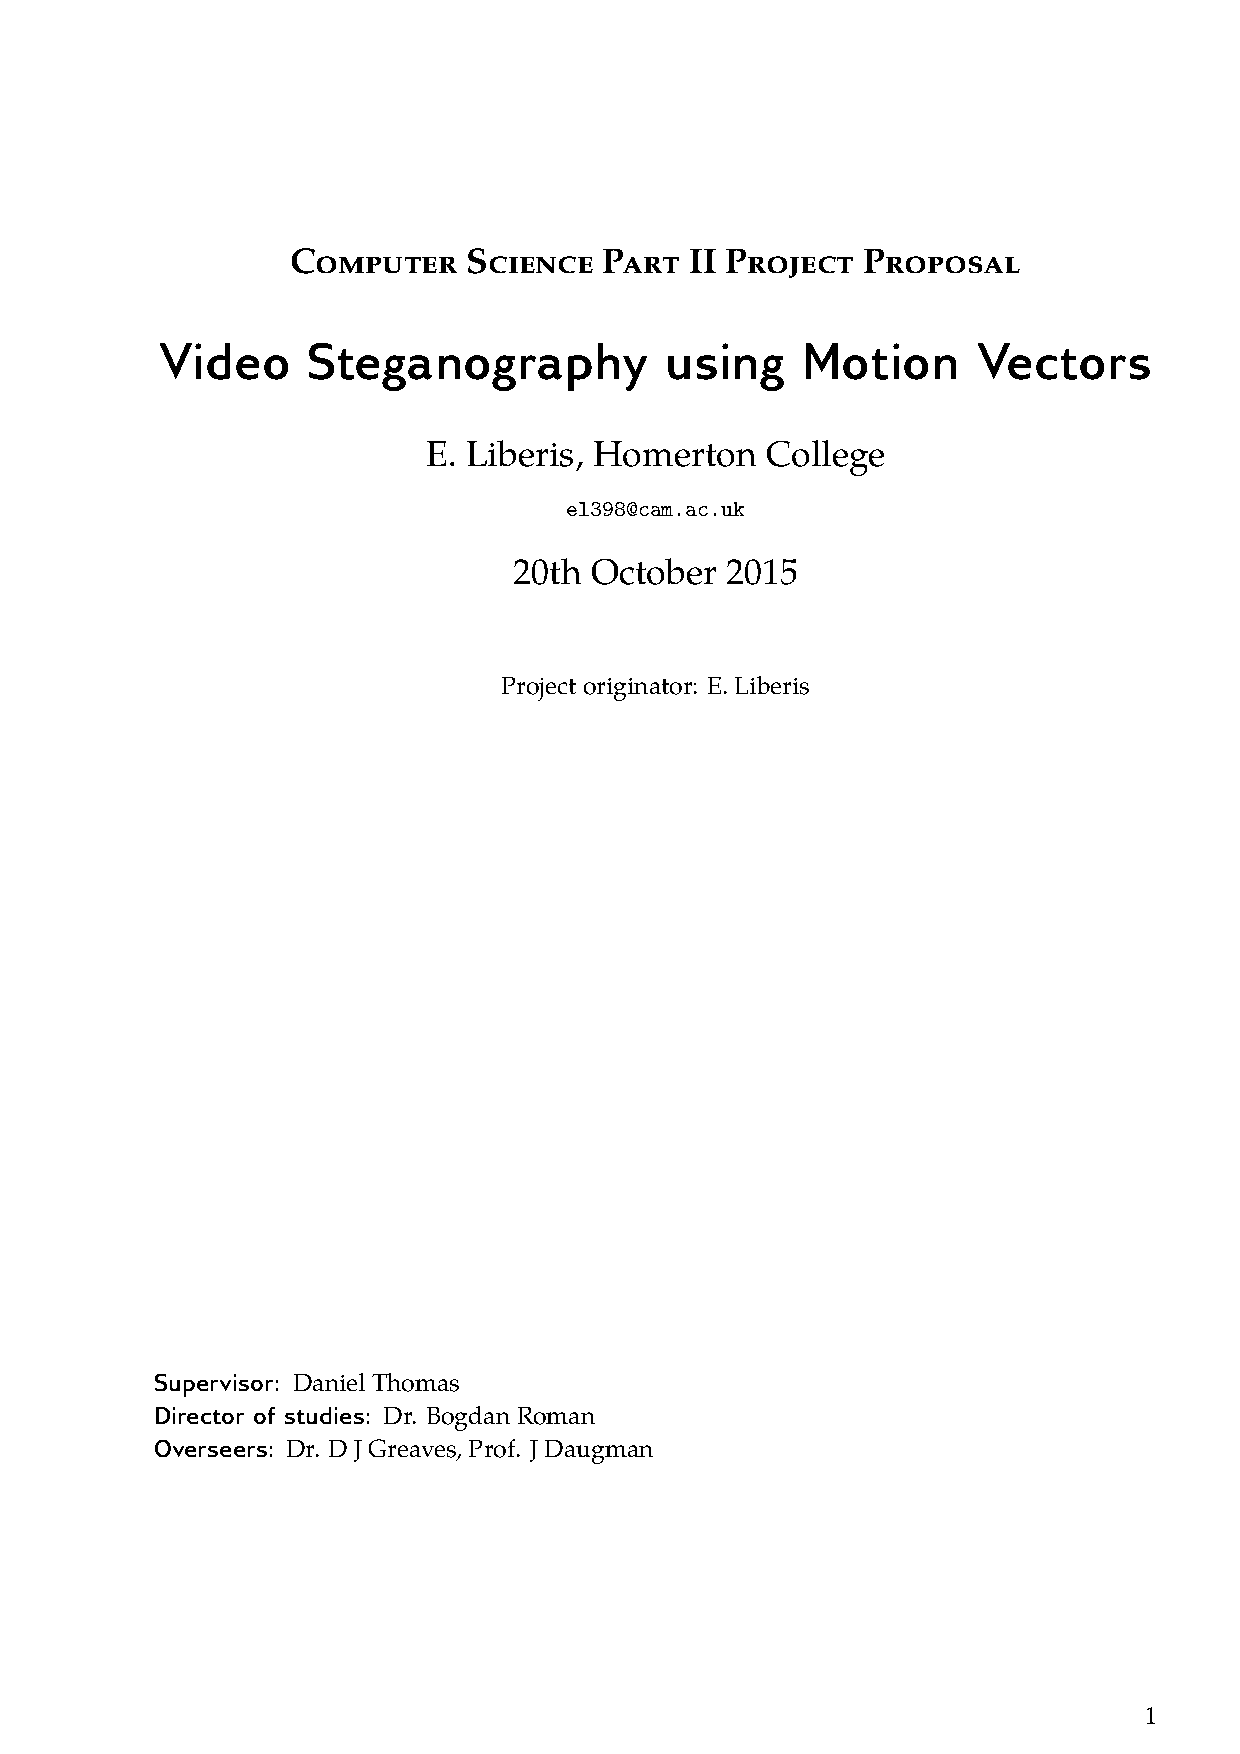
\includepdf[pages={-}]{proposal.pdf}


\end{document}